

\documentclass[final]{phduio} % Bruk [colophon] for å lage cover-print. Use [final] for printing. Den står i motsetning til [draft], som tilsynelatende er standard i klassen phduio.

\usepackage{phdstyle}   % Custom style
\usepackage{kantlipsum} % Dummy text

\author{Rune Vegard Skullerud Fjellbo}
\title{Non-singular simplicial sets}
\department{Department of Mathematics}
\faculty{The Faculty of Mathematics and Natural Sciences}

\affiliation
{
    University of Oslo
    % \and
    % Optional Further Specification
}
\ISSN{1234-5678}
\dissertationseries{1234}



\includeonly
{
    chapters/abstract,
    chapters/dedication,
    % chapters/declaration,
    chapters/acknowledgements,
    chapters/reader,
    chapters/introduction,
    chapters/itdesing,
    chapters/exponentials,
    chapters/model,
    chapters/technical,
    chapters/htythy,
    chapters/optriang,
    chapters/cofibrantobj,
    % chapters/appendixA,
    % chapters/appendixB,
}

\begin{document}

    \frontmatter        % Folios in Roman numerals, unnumbered chapters.
    
    \uiotitle
    

    % \abstractintoc % Add abstract to Table of Contents  
%\abstractnum  % Format abstract like a chapter

\begin{abstract}

\noindent A simplicial set is said to be \textbf{non-singular} if its non-degenerate simplices are embedded. Let $sSet$ denote the category of simplicial sets. We prove that the full subcategory $nsSet$ whose objects are the non-singular simplicial sets admits a model structure such that $nsSet$ becomes is Quillen equivalent to $sSet$ equipped with the standard model structure due to Quillen \cite{Qu67}. The model structure on $nsSet$ is right-induced from $sSet$ and it makes $nsSet$ a proper cofibrantly generated model category. Together with Thomason's model structure on small categories \cite{Th80} and Raptis' model structure on posets \cite{Ra10} these form a square-shaped diagram of Quillen equivalent model categories in which the subsquare of right adjoints commutes.










\noindent Simplicial sets has a standard model structure due to Quillen in which the weak equivalences are the morphisms whose geometric realizations are weak homotopy equivalences and in which the fibrations are the Kan fibrations. A simplicial set is non-singular if its non-degenerate simplices are embedded. The inclusion of the full subcategory of non-singular simplicial sets into the category of simplicial sets has a left adjoint, referred to under the name desingularization.

The Kan subdivision has a right adjoint, called extension. The double subdivision followed by desingularization is then left adjoint to the inclusion followed by the double extension. Inspired by Thomason \cite{Th80}, we lift the standard model structure on simplicial sets to non-singular simplicial sets by letting a morphism be a weak equivalence (fibration) whenever it becomes a weak equivalence (fibration) after applying the inclusion followed by the double extension. Thus non-singular simplicial sets is a proper cofibrantly generated (closed) model category and the double (Kan) subdivision followed by desingularization is the left Quillen functor of a Quillen equivalence.

The category of non-singular simplicial sets is of interest in piecewise linear topology, and sits strictly between ordered simplicial complexes and simplicial sets. As a model for spaces, the older (ordered) simplicial complexes are more directly put into the modern context of model categories by our model structure on non-singular simplicial sets.

A difficulty when attempting to lift the model structure on simplicial sets to the non-singular ones is that the only known description is non-concrete. Part of this thesis is to work around that. A noteworthy result in that regard is that the operation of taking a product with a non-singular simplicial set is an endofunctor of non-singular simplicial sets that preserves colimits.
    
Asking for a characterization of the cofibrant objects in the obtained model structure on non-singular simplicial sets leads to whether the Barratt nerve is the optimal triangulation of regular simplicial sets. Put precisely, one is lead to ask whether the natural map from the desingularized subdivision to the Barratt nerve is an isomorphism in the case when the simplicial set is regular. Waldhausen expects an affirmative answer to this question, which is put forward by Waldhausen, Jahren and Rognes \cite{WJR13}. Indeed, our third major result is a confirmation of Waldhausen's suspicion. As a consequence, the improvement functor used in \cite{WJR13} to make simplicial sets non-singular is not at all ad hoc and has even better properties than previously known. The improvement functor is by definition Kan subdivision followed by the Barratt nerve.
\end{abstract}




    \chapter{Dedication}

The women in my life have taken care of themselves lately. Of that they are more than capable. However, I hope to be around more from now on. Sofia was kind enough to go swimming with me for three quarters of a year during the most hectic period of my PhD candidacy. This weekly happening renewed my focus and made the workweek brighter. Although she learned how to walk a year and a half ago, she is still dependent on others to prepare her meals. The burden fell on her mother who also prepared most of mine.

Most humble of all thanksgivings is the one I direct towards Anisa. To convey the academic achievements of the PhD candidacy at the level I have managed, would not at all have been possible if she was any less patient. By her grace, I have been allowed to neglect parts of my share of the parenthood and of the household. She, on the other hand, took a larger share herself and furthermore organized the efforts made by the other people in our lives. Things are about to become different.

To have Anisa and Sofia in my life adds to the meaning of the PhD candidacy and has increased the motivation to finish in a good way. I am thankful to them both.



    % \chapter{Declaration}

\noindent
To the best of the PhD candidate's knowledge, the following achievement is my own. Any work that is not mentioned here in this declaration is likely not original, or in other words someone else's. In that case, said work is just part of this written presentation to make the story as self-contained as possible. I trust that I have held a reasonable account of references.

There are three results that are my own.

My first result is that one can talk about the simplicial mapping set in the category of non-singular simplicial sets. The need for such a result came up during the work to establish my second result. Rather, it is sufficient to be able to talk about simplicial path sets. This special case is by far the most work intensive part of the proof. My supervisor, John Rognes, had at an earlier time asked himself whether simplicial mapping sets make sense in the category of non-singular simplicial sets, though with another application in mind.

My second result is that the standard model structure on simplicial sets that is due to Quillen, in which the weak equivalences are those that induce weak homotopy equivalences and the fibrations are the Kan fibrations, can be lifted across the inclusion followed by double extension, which is right adjoint to twice Kan's subdivision. The style of lifting is a standardized method due to Kan. Largely, the ideas that make the lifting possible come from theory of regular neighborhoods. The choice of Kan's double subdivision followed by desingularization as the homotopy inverse of the inclusion is of course barrowed by Thomason \cite{Th80}. I also barrow his idea of using an auxiliary class of morphisms to aid in the lifting. His term Dwyer morphism was a source of inspiration in that regard, but even more so were Cisinski's correction \cite{Ci99} of Thomason's mistake and a characterization of cofibrations in topological spaces due to Strøm \cite{St66}.

My third result is that Kan's subdivision performed twice followed by desingularization and Kan's subdivision followed by the Barratt nerve are one and the same (up to a natural isomorphism). Waldhausen, Jahren and Rognes (my supervisor) believed in this statement, but used the latter construction rather than the former as a tool in their work \cite{WJR13} as they did not have a proof. Thomason's term Dwyer map \cite{Th80} was useful in one of the steps I took to reduce the problem to its core. Theory of mapping cylinders is very close to this as it is a special case, but I feel that the term Dwyer map most appropriately captures the relevant structures in that step of the problem reduction. In said step I also use a result by Thomason and even a technique from a proof of another result, both from the same article \cite{Th80}.

Furthermore, the reader may notice that I have provided an alternative description of desingularization. This is not quite original as it resembles how Lewis \cite[pp.~158]{Le78} made a space Hausdorff, essentially by identifying two points until a quotient with the Hausdorff property emerges. However, I did more or less make my description of desingularization before my advisor told me of the work of Lewis. When I did learn of his construction I decided to match the method and notation with his, to a certain extent, for comparison.
    
\chapter{Acknowledgements}

First and foremost I want to thank John who gave me the opportunity to work with this project. It has been very rewarding in and of itself. However, during my time as a PhD candidate I have also had the opportunity to expose myself to many interests that a less independent position would likely be an obstacle to. John is demanding when delivering criticism, but he is also patient and has given me great freedom. He has also encouraged me to give talks and has supervised me in seminars and in self taught topics.

Although I had hoped to explore more of the questions that were posed during my time at the department, it seems that there is after all quite a lot of publishable material at the moment this is written. Moreover, the material has taken shape as four individual papers that form four chapters in this thesis that are formulated in a more independent manner than the rest. John put down a lot of work to help me with the final (?) formulation of the publishable work. Now I feel more than ready to move on to a new period of my life --- an existence that I hope involves some mathematics, although of a slightly more practical nature.

Most of my courses above a certain level were taught by Paul Arne and Bjørn. Paul Arne has a style of teaching that comes with great reward as there is often a lot of effort put into say the problem solving sessions. Bjørn has geometrical insights and experience that I could never extract from any book. The courses they both taught were highly appreciated.

The department administration has been a tremendous help, for example the staff shields the scientific staff from the outside world and is also a bridge to it when it is desired or necessary. Help is immediately available at all times, and links are provided to experts in the faculty staff that can help with say legal matters. It is particularly Yngvar and Biljana that deserve praise in this regard.

The office computer and the software is as stable as I have ever experienced. Any request concerning IT is dealt with superbly and shortly after making contact. If there is ever a problem, then Terje will fix it, handing out new equipment if he has to. I doubt that there is a better supporting staff than the one at the Math. dept.

Karoline was very helpful as she started working in the library, but first and foremost she was a friend and colleague before and after that point in time. Similarly, I shared hallway with Sigurd who has also been a friend and colleague during my time at the department --- one who helped me with the programming of illustrations in LaTeX. Martin provided me with the template in which this is written, which worked excellent and better than anything I used before.

My mother and father have been supportive in everything I ever did --- in all possible aspects. The PhD candidacy is no exception. To have them has been very important, even essential after I established a home and later a family. My daughter gets from them what I myself cannot manage in this hectic and somewhat irregular existence --- and more. Especially my mother deserves thanks as she travels far just to be with her. Concerning my daughter, an even greater role than my mother's is played in daily life by her aunt Nimo. She is like a third parent. Not to mention the fact that she helped us a lot in the period before Sofia was born. It is an understatement to say that she has been there for us beyond the call of duty. I am deeply thankful to her.

More people could certainly have been mentioned here. Furthermore, I have made a few friends for life during my stay at the department. This is yet another by-product of getting the opportunity that the PhD candidacy has been.


    
\chapter{To the reader}

The author’s PhD thesis grew out of the desires, firstly to establish an interesting model structure on non-singular simplicial sets with a connection to simplicial sets that uses the desingularization functor, and secondly to describe desingularization. As a product of this work, the author proved four major results. Each of these theorems developed into a self-contained text that the author intends to try to publish. Therefore, this dissertation is not quite a monograph, but rather four attemped articles with connections between them and with a surrounding text that supports them so as to supplement the material and make all of the material readable in a suitable context. The four articles are the chapters \ref{ch:it_desing},\ref{ch:exponentials},\ref{ch:htythy} and \ref{ch:optriang}. Consequently, there may be advantages and disadvantages for the reader, compared with reading a monograph. 

Presumably, there are two possible minimum requirements for reading this dissertation. A master student with some prior knowledge of simplicial sets and of model categories should be able to read the dissertation. So too, should a more experienced topologist that is familiar with homotopy theory, but without prior knowledge of model categories. \cref{ch:model} is a minimal treatment of model categories. For a master student with prior knowledge, this chapter serves to fix notation and terminology. On the other hand, a more experienced topologist that is familiar with homotopy theory, is likely to surmise the motivation behind model structures by reading \cref{ch:model}. 

One possible disadvantage with reading this hybrid between a monograph and an article-based dissertation is that some material is repeated, in order to make the four chapters \ref{ch:it_desing},\ref{ch:exponentials},\ref{ch:htythy} and \ref{ch:optriang} self-contained. 

A possible advantage is the opportunity to read any of the three articles in chapters \ref{ch:it_desing},\ref{ch:exponentials} or \ref{ch:optriang} without looking at the other material prior to the reading. The reason that this is possible is that the number of references out of the four attempted articles is kept to a minimum. As such, it is realistic to immediately read any one of the chapters \ref{ch:it_desing},\ref{ch:exponentials} or \ref{ch:optriang} with the occational glance at the few external references.

However, to read \cref{ch:htythy}, one might want read \cref{ch:model} first, because \cref{ch:htythy} concerns the establishing of a model structure on non-singular simplicial sets, and \cref{ch:model} is our minimal treatment of model categories. In the event that the reader is already familiar with Hirschhorn's or Hovey's book, \cref{ch:model} can be skipped and then looking up the occational reference if needed.

Another possibility is to just read the chapters in order. This is likely to be more rewarding. \cref{ch:htythy} builds on \cref{ch:it_desing} and \cref{ch:exponentials}, whereas \cref{ch:optriang} builds on \cref{ch:htythy}.

Reading any of the chapters in the complement of the chapters \ref{ch:it_desing},\ref{ch:exponentials},\ref{ch:htythy} and \ref{ch:optriang} out of context is not particularly meaningful, as the complement is simply there to supplement the four attempted articles.



    \cleartorecto
    \tableofcontents    % Or \tableofcontents*
    \cleartorecto
    \listoffigures
    \cleartorecto
    \listoftables
    

    \mainmatter         % Folios in Arabic numerals, numbered chapters.
    
    % How should I organize the thesis? There is publishable and non-publishable
    % material. Moreover, it would be convenient if each publishable result is
    % a chapter in this project
    % with an abstract, introduction and so on, as usual. This chapter should be
    % the main chapter of a part. Then it is possible to supplement the chapter with
    % extra details, formal reasoning, examples and non-examples, etc. However,
    % the chapters that are articles will be long, probably longer than most.
    % Thus they should probably be subdivided into sections. I should test how this
    % can be done, technically. The problem is that I do not yet know which chapters
    % will be the articles. This is maybe a good reason to give the chapters
    % descriptive names for myself, but the chapters should still have numbers
    % that are not related to the subdivision into parts.

    \chapter{Introduction}
\label{ch:intro}

\noindent Combinatorial structures on topological spaces can be a useful tool. Highly relevant to this day are simplicial complexes. They were invented by Poincaré in the late 19th century, though Alexandroff fully clarified the notion in 1925 \cite{Al25}. Although possible, it is in general not meaningful to form limits and colimits of diagrams of simplicial complexes. We mean this in the sense that neither limits nor colimits are preserved by geometric realization. The reason for this phenomenon is the high rigidity of the rules of the glueing of simplices.

Relaxing the rules of glueing leads to the concept of simplicial set. This was introduced in 1950 by Eilenberg and Zilber \cite{EZ50} under the name of \emph{semi-simplicial complexes}. A common viewpoint is that simplicial sets $X$ are graded sets $X=\bigsqcup _{n\geq 0}X_n$ that come with face maps $d_i:X_n\to X_{n-1}$, $0\leq i\leq n$, and degeneracy maps $s_j:X_n\to X_{n+1}$, $0\leq j\leq n$, that specify the result of omitting the $i$-th vertex or repeating the $j$-th vertex, respectively.

To make a connection between the older simplicial complexes $SiCo$ and the newer simplicial sets one can adjust the definition by demanding that the vertices of a simplex belonging to a simplicial complex is a totally ordered set. Then it makes sense to refer to the $i$-th vertex of a simplex, and to the $i$-th face, which is the simplex one gets by removing the $i$-th vertex.

Let $OSiCo$ denote the category of these ordered simplicial complexes. Because of the numbering of vertices of each simplex $OSiCo$ embeds as a full subcategory of simplicial sets. There is also an interesting functor $SiCo\to OSiCo$ known as barycentric subdivision, which plays a role in this thesis.

Consider the diagram of adjunctions in \cref{fig:Square_adjunctions}, in which there are three categories that often occur in the literature. Namely, we have $sSet$, which is the category of simplicial sets, we have $Cat$, which is the category of small categories and we have $PoSet$, which is the category of partially ordered sets (posets). One of the categories almost never occur in the literature, however. A simplicial set is \textbf{non-singular} if the representing map of each non-degenerate simplex is degreewise injective. We let $nsSet$ denote the full subcategory of $sSet$ whose objects are the non-singular simplicial sets. The category $nsSet$ is strictly between $sSet$ and $OSiCo$, as we explain in \cref{sec:intro_hty}.

\begin{figure}
\centering
\begin{tikzcd}
&& sSet \ar[ld,"Sd^2"',shift right=0.5ex] \\
Cat \ar[d,"p"',shift right=0.5ex] \ar[r,"N"',shift right=0.5ex] & sSet \ar[l,"c"',shift right=0.5ex] \ar[d,"D"',shift right=0.5ex] \ar[ur,"Ex^2"',shift right=0.5ex] \\
PoSet \ar[u,"U"',shift right =0.5ex] \ar[r,"N"',shift right=0.5ex] & nsSet \ar[l,"q"',shift right=0.5ex] \ar[u,"U"',shift right=0.5ex]
\end{tikzcd}
\caption{Diagram of adjunctions.}
\label{fig:Square_adjunctions}
\end{figure}

Non-singular simplicial sets play a role in the book \cite{WJR13} by Waldhausen, Jahren and Rognes. The reason is that they have a natural piecewise linear (PL) structure \cite[§3.4]{WJR13}.

In this thesis we consider two model structures on $sSet$. The first is the standard model structure on $sSet$ due to Quillen \cite{Qu67}. The second is a model structure introduced by J. F. Jardine \cite{Ja13}. One can use the Kan subdivision, denoted $Sd$, and its right adjoint, sometimes referred to as extension and denoted $Ex$, to shift the fibrations and cofibrations so that the fibrations become more abundant. This operation can be iterated. For example, the Kan subdivision performed twice becomes a left Quillen functor, of the Quillen equivalence $(Sd^2,Ex^2)$, whose source is $sSet$ equipped with Quillen's structure and whose target is $sSet$ equipped with Jardine's structure \cite[Thm.~1.1.,~p.~274]{Ja13}.

Using ideas from regular neighborhood theory \cite[§II]{Hu69}, Thomason managed to lift Quillen's structure to $Cat$ along $Ex^2N$ \cite{Th80}, where $N:Cat\to sSet$ is the standard nerve functor \cite[§2]{Se68}. The result was that $Cat$ became a proper cofibrantly generated model category and that the adjunction $(cSd^2,Ex^2N)$ became a Quillen equivalence. As a consequence, the adjunction $(c,N)$ is a Quillen equivalence when $sSet$ has Jardine's $Sd^2$-model structure. Much later, Raptis restricted Thomason's model structure to posets \cite{Ra10}. The functors denoted $U$ in \cref{fig:Square_adjunctions} are inclusions and the subsquare of right adjoints commutes precisely.

In this thesis, we adapt Thomason's method to the setting of non-singular simplicial sets and prove an analogous result, namely that $nsSet$ is a proper cofibrantly generated model category and that $(DSd^2,Ex^2U)$ is a Quillen equivalence. The functor $c$, often called categorification, has an elementary description, but the functor $D$ \cite[Rem.~2.2.12]{WJR13}, called desingularization, does not. Here lies a potential difficulty in trying to establish a model structure on $nsSet$ that is Quillen equivalent to $sSet$ equipped with Quillen's model structure. Thomason's auxiliary morphisms known as Dwyer maps are used as a source of inspiration in establishing $(DSd^2,Ex^2U)$ is a Quillen equivalence, which is stated as \cref{thm:main_homotopy_theory}. \cref{ch:htythy} is more or less devoted to this result.

Using the chosen strategy to establish \cref{thm:main_homotopy_theory} made it necessary to understand how desingularization behaves when applied to certain sensibly formed quotients of non-singular simplicial sets and to certain finite products. Out of these tasks grew the work of \cref{ch:it_desing} and \cref{ch:exponentials}. Specifically, we use techniques from the work to establish \cref{thm:main_result_itdesing} and we use \cref{cor:take_product_cocontinous_endofunctor_non-singular} directly in the proof of \cref{thm:main_homotopy_theory}.

For the reader that is familiar with homotopy theory, but not with the language of model categories, we try to mend this eventuality in \cref{ch:model}. The chapter also serves to fix notation and terminology.

\cref{ch:technical} deals with some technical aspects of the category of non-singular simplicial sets. As one might expect, the inclusion $U:nsSet\to sSet$ preserves filtered colimits. We prove this in \cref{sec:smallness} --- a fact that is used several places in the dissertation. The final section of \cref{sec:formal} is devoted to the folklore that a non-singular simplicial set can be glued together over its non-degenerate simplices.

Calculations done in \cref{sec:examples} suggests that the left Quillen functor $DSd^2$ might be naturally isomorphic to the improvement functor from \cite[Thm.~2.5.2]{WJR13}, which is also explicitly and implicitly the topic of most of the exercises in Section $4.6$ of \cite[pp.~219--220]{FP90}. The question was raised in \cite[Rem.~2.2.12]{WJR13}. We answer it in the affirmative by stating \cref{thm:main_opt_triang}. The result is derived from \cref{thm:barratt_nerve_rep_map_dcr_iso}, which is interesting in its own right as it seems to bring new knowledge concerning the reduced mapping cylinder from \cite[§2.4]{WJR13}.

Having established \cref{thm:main_homotopy_theory} there are many questions that can be raised. For example, is every cofibrant non-singular simplicial set the nerve of some poset? The statement seems analogous to a result by Thomason \cite[Prop.~5.7]{Th80}. There are reasons to think that the answer is yes and we state the informed guess as \cref{conj:cofibrant_nonsing_simp_set}. \cref{ch:sixth} is largely devoted to justify this. Parts of \cref{ch:sixth} goes beyond a justification for \cref{conj:cofibrant_nonsing_simp_set}, however, and is instead speculative. In fact, the chapter becomes increasingly speculative towards the end. \cref{sec:simplexcat} consists of constructions and speculations. The only construction therein that is of value to the justification is the construction of $c$, which we make light use of in the proof of \cref{prop:categorification_of_DSd_vs_B}.








	% Behavior of desingularization in the presence of various colimits, properties
	% of the category of non-singular simplicial sets, including the construction
	% of simplicial mappings sets. Formalities regarding reflective subcategories,
	% locally presentable categories, etc.
    \part{Desingularization}

    
\chapter{Iterative desingularization}
\label{ch:it_desing}



\begin{abstract}
\noindent A simplicial set is said to be \textbf{non-singular} if the representing map of each non-degenerate simplex is degreewise injective. The inclusion into the category of simplicial sets, of the full subcategory whose objects are the non-singular simplicial sets, admits a left adjoint functor called desingularization. In this paper, we provide an iterative description of desingularization that is useful for theoretical purposes as well as for doing calculations.
\end{abstract}


\section{Introduction}
\label{sec:intro_itdesing}

Desingularization is defined thus.
\begin{definition}\label{def:desingularization}
Let $X$ be a simplicial set. The \textbf{desingularization} of $X$ \cite[Rem.~2.2.12]{WJR13}, denoted $DX$, is the image of the map
\[X\to \prod _{f:X\rightarrow Y}Y\]
given by $x\mapsto (f(x))_f$, where the product is indexed over the quotient maps $f:X\rightarrow Y$ whose targets $Y$ are non-singular.
\end{definition}
\noindent A product of non-singular simplicial sets is again non-singular\\ \cite[Rem.~2.2.12]{WJR13}, and a simplicial subset of a non-singular simplicial set is again non-singular \cite[Rem.~2.2.12]{WJR13}. Therefore, the simplicial set $DX$ is non-singular. In this paper, we will give a systematic, but minimal introduction to the functor $D$.

If we corestrict the map $X\to \prod _{f:X\rightarrow Y}Y$ to its image $DX$, then we get a map $\eta _X:X\to DX$. By this we simply mean the following. If $h:Z\to W$ is a simplicial map whose image is contained in some simplicial subset $W'$ of $W$, then we say that the induced map $Z\to W'$ is a \textbf{corestriction} of $h$ to $W'$.

Thus far, the description given in \cref{def:desingularization} is the only description available in the literature. In this paper, we provide the viewpoint of \cref{thm:main_result_itdesing} to desingularization. To obtain this viewpoint, we introduce the notion of enforcer in \cref{def:enforcer}.

When we say that a simplex is \textbf{embedded} if its representing map is degreewise injective, we get a more convenient definition of the term \emph{non-singular simplicial set}. Given a simplicial set $X$ and a non-degenerate simplex $x$ in $X$, the enforcer $\rho _x$ is the degeneracy operator that in the least drastic way makes the cobase change of the representing map of $x$ into the representing map of a degenerate simplex, in the case when $x$ is not embedded, or that makes the trivial cobase change, in the case when $x$ is embedded. In other words, the enforcer is the degeneracy operator that is as close as possible to the identity meanwhile honouring any pairwise equalities between the vertices of $x$.

Simultaneously pushing out along all the enforcers associated with a simplicial set $X$ yields a simplicial set $Cen(X)$ that we refer to as the enforced collapse of $X$. The notion is properly introduced in \cref{def:enforced_collapse}. One should think of the enforced collapse as a preferred first step towards making $X$ non-singular. If some non-degenerate simplex of $X$ is not embedded, then we say that $X$ is \textbf{singular}. Note that $Cen(X)$ may be singular. By \cref{lem:pushout_along_enforcers_intermediate_desingularization}, which is formulated in a slightly generalized context compared with the enforced collapse, we get that pushing out along enforcers is never too drastic. Moreover, if the result is non-singular, then it is canonically the desingularization.

We are ready to explain the iterative description of desingularization, which is formulated using the following piece of language.
\begin{definition}\label{def:sequence_composition}
Let $\mathscr{C}$ be some cocomplete category and suppose $\lambda$ some ordinal. A \textbf{$\lambda$-sequence in $\mathscr{C}$} is a cocontinous functor $X:\lambda \to \mathscr{C}$, that we will denote
\begin{displaymath}
\xymatrix{
X^{[0]} \ar[r]^{f^{0,1}} & X^{[1]} \ar[r]^{f^{1,2}} & \cdots \ar[r] & X^{[\beta ]}\ar[r]^{f^{\beta ,\beta +1}} & \cdots \, .
}
\end{displaymath}
The canonical map $X^{[0]}\to colim_{\beta <\lambda }X^{[\beta ]}$ is the \textbf{composition} of the $\lambda$-sequence. A \textbf{sequence} in $\mathscr{C}$ is a $\lambda$-sequence for some $\lambda$.
\end{definition}
\noindent If $\lambda$ is finite, then the composition is a composite in the usual sense.
\begin{theorem}\label{thm:main_result_itdesing}
Let $X$ be a simplicial set. There is an ordinal $\lambda$ such that the map $\eta _X:X\to UDX$ is the composition of the $\lambda$-sequence
\begin{displaymath}
\xymatrix{
Cen^0(X) \ar[r] & Cen^1(X) \ar[r] & \cdots \ar[r] & Cen^\beta (X) \ar[r] & \cdots \, .
}
\end{displaymath}
of iterations of the enforced collapse.
\end{theorem}
\noindent \cref{thm:main_result_itdesing} provides an alternative description of the desingularization functor. Note that the ordinal $\lambda$ depends on the simplicial set $X$.

Let $sSet$ denote the category of simplicial sets. Furthermore, let $nsSet$ denote the category of non-singular simplicial sets. It is by definition the full subcategory of $sSet$ whose objects are the non-singular simplicial sets.

As we explain \cref{def:desingularization} and as we explain how desingularization is functorial in \cref{sec:prelim}, we fix some notation and terminology to be used throughout the paper. Furthermore, we point out the implications for limits and colimits in $nsSet$ of the fact that $D$ is left adjoint to the (full) inclusion $U:nsSet\to sSet$. \cref{sec:prelim} is merely an elaboration of \cite[Rem.~2.2.12]{WJR13}, where desingularization is introduced.

In \cref{sec:calculations}, we introduce the enforcer to serve as the most basic technology for doing calculations as well as for theory. Building on this notion, we provide the two results \cref{prop:role_of_enforcers} and \cref{lem:pushout_along_enforcers_intermediate_desingularization} as tools.

We illustrate how desingularization behaves in \cref{sec:examples}. Our examples include applying $D$ to highly singular, somewhat subdivided and very subdivided simplicial sets, most of which are models of low-dimensional spheres.

Finally, in \cref{sec:description}, we explain how \cref{prop:role_of_enforcers} and \cref{lem:pushout_along_enforcers_intermediate_desingularization} can be used to construct the sequence that \cref{thm:main_result_itdesing} refers to and we conclude the section as well as the paper by deducing \cref{thm:main_result_itdesing} from the construction.





\section{Preliminaries}
\label{sec:prelim}

In this section, we establish the functorality of desingularization. To do this, we first fix some basic notation and terminology, which is anyhow useful throughout this paper. Additionally, we properly explain \cref{def:desingularization} to avoid any confusion.

\subsection{Notation and terminology}

Fritsch and Piccinini \cite{FP90} is a source of the style we use, when it comes to notation and terminology.

The category
\[sSet=Fun(\Delta ^{op},Set)\]
is the category of functors (and natural transformations) with source $\Delta ^{op}$ and target the category $Set$ of sets (and functions). When we write $\Delta$, we mean the skeleton of finite ordinals whose objects are totally ordered sets
\[[n]=\{ 0<1<\dots <n\}\]
and whose morphisms are order-preserving functions $\alpha :[m]\to [n]$, meaning $\alpha (i)\leq \alpha (j)$ if $i\leq j$. An object in the category $sSet$ is a \textbf{simplicial set}.

Morphisms of $\Delta$ are referred to as \textbf{operators}. We sometimes think of a simplicial set $X$ as an $\mathbb{N} _0$-graded set $\bigsqcup _{n\geq 0}X_n$ with operators acting from the right. Here, we mean $X_n=X([n])$, $n\geq 0$. Elements of $X_n$ are referred to as \textbf{$n$-simplices}, $n\geq 0$. We also say that $n$ is the \textbf{degree} of $x$ if $x$ is an $n$-simplex. If $x$ is an $n$-simplex of $X$ and if $\alpha :[m]\to [n]$ is an operator, then $\alpha$ acts on $x$ from the right. The result will be denoted $x\alpha$. The induced function $\alpha ^*:X_n\to X_m$ thus takes $x$ to $\alpha ^*(x)=x\alpha$.

When we think of simplicial sets as graded sets under right action of operators, we also think of a simplicial map $f:X\to Y$, meaning a natural transformation $X\Rightarrow Y$, as a function that respect the degree, meaning $f(x)\in Y_n$ if $x\in X_n$, and that is compatible with the right action of operators, meaning $f(x\alpha )=f(x)\alpha$.

An operator $\alpha :[m]\to [n]$ is referred to as a \textbf{face operator} if $\alpha (i)\neq \alpha (j)$ whenever $i,j\in \{0,\dots ,m\}$ and $i\neq j$. It is referred to as a \textbf{degeneracy operator} if $k=\alpha (j)$ for some $j\in \{0,\dots ,m\}$ for all $k\in \{0,\dots ,n\}$. These classes of morphisms are precisely the monomorphisms and epimorphisms of $\Delta$, respectively.

For each $n>0$ and each $j$ with $0\leq j\leq n$, we can define the face operator $\delta ^n_j:[n-1]\to [n]$ such that $j$ is not in its image, referred to as an \textbf{elementary face operator}. Similarly, for each $n\geq 0$, we can define the degeneracy operator $\sigma ^n_j:[n+1]\to [n]$ with $j\mapsto j$ and $j+1\mapsto j$. Also useful is the \textbf{vertex operator} $\varepsilon ^n_j:[0]\to [n]$ with $0\mapsto j$, defined whenever $0\leq j\leq n$. We often omit the upper index when referring to these three special types of operators.

A degeneracy operator or face operator is \textbf{proper} if it is not an identity morphism. We say that a simplex $y$ is a \textbf{(proper) face} of a simplex $x$ if $y=x\mu$ for some (proper) face operator $\mu$ and that $y$ is a \textbf{(proper) degeneracy} of $x$ if $y=x\rho$ for some (proper) degeneracy operator $\rho$. A simplex is \textbf{non-degenerate} if it is not a proper degeneracy. 

The Eilenberg-Zilber lemma \cite[Thm.~4.2.3]{FP90} says that any simplex $x$ of a simplicial set can be written uniquely as a degeneration of a non-degenerate simplex. This means that there is a unique pair $(x^\sharp ,x^\flat )$ consisting of a non-degenerate simplex $x^\sharp$ and a degeneracy operator $x^\flat$ that satisfies
\[x=x^\sharp x^\flat.\]
The non-degenerate simplex $x^\sharp$ will be referred to as the \textbf{non-degenerate part} of $x$ and $x^\flat$ will be referred to as the \textbf{degenerate part} of $x$. We let $X^\sharp$ denote the set of non-degenerate simplices of a simplicial set $X$ and $X^\sharp _n$ the set of non-degenerate simplices of degree $n$, for each $n\geq 0$.

By the Yoneda lemma, there is a natural bijective correspondence $x\mapsto \bar{x}$ between the set $X_n$ of $n$-simplices and the set of simplicial maps $\Delta [n]\to X$. We say that
\[\bar{x}:\Delta [n]\to X\]
is the \textbf{representing map} of the simplex $x$.


\subsection{Quotients}

Desingularization has the following property \cite[Rem.~2.2.12]{WJR13}.
\begin{lemma}\label{lem:desing_unique_factorization_through_unit}
Let $X$ be a simplicial set. Every simplicial map whose source is $X$ and whose target is non-singular factors uniquely through $\eta _X$.
\end{lemma}
\noindent Before we prove the property, we explain \cref{def:desingularization} properly.

Let $X$ be some simplicial set. Consider the event that we for each $n\geq 0$ have an equivalence relation $R_n$ on $X_n$ such that whenever we have an operator $\alpha :[m]\to [n]$, then the composite
\[R_n\to X_n\times X_n\xrightarrow{\alpha ^*\times \alpha ^*} X_m\times X_m\]
corestricts to $R_m\subseteq X_m\times X_m$. This means that we have a commutative square
\begin{equation}
\label{eq:first_diagram_proof_lem_desing_unique_factorization_through_unit}
\begin{gathered}
\xymatrix{
R_n \ar[d]_{\bar{\alpha } } \ar[r] & X_n\times X_n \ar[d]^{\alpha ^*\times \alpha ^*} \\
R_m \ar[r] & X_m\times X_m
}
\end{gathered}
\end{equation}
which in turn gives rise to a dashed map in the square
\begin{equation}
\label{eq:second_diagram_proof_lem_desing_unique_factorization_through_unit}
\begin{gathered}
\xymatrix{
X_n \ar[d]_{\alpha ^*} \ar[r] & X_n/R_n \ar@{-->}[d] \\
X_m \ar[r] & X_m/R_m
}
\end{gathered}
\end{equation}
such that it commutes.

Thus we obtain a simplicial set $X/R$ given by defining the set
\[(X/R)_n=X_n/R_n\]
as the set of $n$-simplices. It is readily checked that the right hand vertical map in (\ref{eq:second_diagram_proof_lem_desing_unique_factorization_through_unit}) is a right action of the operator $\alpha$ on the set $X_n/R_n$ so that $X/R$ is indeed a simplicial set. From the commutativity of (\ref{eq:second_diagram_proof_lem_desing_unique_factorization_through_unit}), it is automatic that the canonical map $X\to X/R$ is a simplicial map. We say that it is a \textbf{quotient map}. If we fix a simplicial set $X$, then the quotient maps $X\to Y$ form a set. This explains \cref{def:desingularization}.

If $f:X\to Y$ is a degreewise surjective simplicial map, then we may define $R_n$, $n\geq 0$, by letting $x\sim x'$ if $f(x)=f(x')$. Because $f$ respects operators, as a simplicial map, it follows that the equivalence relations $R_n$, $n\geq 0$, form a set of equivalence relations of the type described above. By making a choice of a representative one can define a map $X/R\to Y$ such that the triangle
\begin{equation}
\label{eq:third_diagram_proof_lem_desing_unique_factorization_through_unit}
\begin{gathered}
\xymatrix{
X \ar[dr] \ar[rr]^f && Y \\
& X/R \ar@{-->}[ur]_\cong
}
\end{gathered}
\end{equation}
commutes. The dashed map is an isomorphism by design. This makes \cref{def:desingularization} meaningful in the sense that we can obtain \cref{lem:desing_unique_factorization_through_unit}. 

We are ready to prove the lemma.
\begin{proof}[Proof of \cref{lem:desing_unique_factorization_through_unit}.]
Let $k:X\to A$ be a map whose target $A$ is non-singular. First, note that there is at most one map $\bar{k}$ such that $k=\bar{k} \circ \eta _X$. This is because $\eta _X$ is degreewise surjective and because the degreewise surjective maps are precisely the epimorphisms of $sSet$ \cite[p.~142]{FP90}. It remains to argue that there is a map $\bar{k}$ such that $k=\bar{k} \circ \eta _X$.

Corestrict $k$ to its image $A'$ so that we get a factorization
\begin{displaymath}
 \xymatrix{
 X \ar[d]_{k''} \ar[dr]^{k'} \ar[r]^k & A \\
 X/R \ar[r]_(.35)\cong & A'=\textrm{Im } k \ar[u]_h
 }
\end{displaymath}
of $k$. Then the map $k'$ is a degreewise surjective map whose target is non-singular. We get the diagram
\begin{equation}
\label{eq:fourth_diagram_proof_lem_desing_unique_factorization_through_unit}
\begin{gathered}
\xymatrix{
& \prod _{f:X\rightarrow Y}Y \ar[dr]^{pr_{k''}} \\
X \ar[ur]^{x\mapsto (f(x))_f} \ar[dr]_{\eta _X} \ar[rr]^(.35){k''} & \ar[u] & X/R \\
& DX \ar@{-}[u] \ar[ur]_g
}
\end{gathered}
\end{equation}
in which we have restricted the projection map
\[\textrm{pr} _{k''}:\prod _{f:X\rightarrow Y}Y\to X/R\]
to $DX$ --- a restriction we denote $g$.

From (\ref{eq:fourth_diagram_proof_lem_desing_unique_factorization_through_unit}) we can conclude that $k''=g\circ \eta _X$ as the outer square and the upper triangle commute. Hence, by the design of $DX$, the map $k'$ factors through the restriction $g$ up to identification with a quotient of $X$ that is isomorphic to $A'$. This yields a factorization of $k$ through $\eta _X$ as the composite
\[X\xrightarrow{\eta _X} DX\xrightarrow{g} X/R\xrightarrow{\cong } A'\xrightarrow{h} A\]
is equal to $k$.
\end{proof}
\noindent If we fix a simplicial set $X$, then we can consider degreewise surjective maps $k:X\to A$ whose targets are non-singular. When factored through $\eta _X$, the resulting unique maps $\bar{k} :DX\to A$ are degreewise surjective. In this sense, desingularization is the least drastic way of forming a non-singular quotient from a (possibly singular) simplicial set.


\subsection{Functorality of $D$ and (co)limits in $nsSet$}

It is possible to define $D$ on morphisms in a straightforward way. Then one realizes that the construction is functorial and that $\eta _X$ is natural as a map $X\to UDX$. If $A$ is non-singular, then $\eta _{UA}$ is an isomorphism. This is observed by factoring the identity $UA\to UA$ through $\eta _{UA}$ by means of \cref{lem:desing_unique_factorization_through_unit}. As $U$ is a full embedding, the latter fact suggests the formulation of \cref{lem:non-singular_reflective_subcategory} below.

A full subcategory of some category is a \textbf{reflective subcategory} if the inclusion admits a left adjoint. The terminology is not quite standard as the fullness assumption is omitted by some, for example in \cite[§IV.3]{ML98} and \cite[p.~1306]{AR15}. As announced, we have the following result \cite[Rem.~2.2.12]{WJR13}.
\begin{lemma}\label{lem:non-singular_reflective_subcategory}
The category of non-singular simplicial sets is a reflective subcategory of $sSet$.
\end{lemma}
\begin{proof}
We will prove the lemma by establishing the natural map $\eta _X$ as the unit of a pair $(\eta ,\epsilon )$ consisting of a unit and a counit $\epsilon$.

Let $f:A\to B$ be a morphism in $nsSet$. Consider the diagram
\begin{displaymath}
 \xymatrix{
 & UD(UB) \\
 && UD(UA) \ar[lu]_{UD(Uf)} \ar[ddr]^{U(\epsilon _A)=\eta ^{-1}_{UA}} \\
 UB \ar[uur]_\cong ^{\eta _{UB}} \\
 & UA \ar[lu]^{Uf} \ar[uur]_\cong ^{\eta _{UA} } \ar[rr]_{id} && UA
 }
\end{displaymath}
in which the inverse $\eta ^{-1}_{UA}$ appears. As $U$ is full, the latter is equal to $U(\epsilon _A)$ for some morphism $\epsilon _A:DU\, A\to A$ of $nsSet$. It is evident from the outer part of the diagram that $\epsilon _A$ is natural in $A$.

The triangle at the right hand side, which defines $\epsilon _A$, is the first half of the compatibility criterion that a unit and a counit must satisfy. The commutative square
\begin{displaymath}
\xymatrix{
 X \ar[d]_{\eta _X} \ar[rr]_{\eta _X} && UDX \ar[d]^{UD(\eta _X)} \\
 UDX \ar[rr]_{\eta _{UDX}}^\cong && UD(UDX)
}
 \end{displaymath}
shows that
\[\eta _{UDX}=UD(\eta _X)\]
for every simplicial set $X$. If we combine this with the definition of $\epsilon _{DX}$, then we get the commutative triangle-shaped diagram
\begin{displaymath}
\xymatrix{
& D(UDX)=DU(DX) \ar[dr]^(.6){\epsilon _{DX}} \\
DX \ar[ur]^(.4){D(\eta _X)} \ar[rr]_{id} && DX
}
\end{displaymath}
which is the second half of the compatibility criterion. This concludes the verification that $D$ is left adjoint to the inclusion $U$.
\end{proof}
\noindent The implication of \cref{lem:non-singular_reflective_subcategory} is that it has a strong bearing on the formation of (co)limits of diagrams in $nsSet$, as we now explain.

A diagram in a reflective subcategory has a limit if it has a limit when considered a diagram in the surrounding category. In that case, the limit is inherited by the subcategory. See for example \cite[p.~92]{ML98} or \cite[p.~1306]{AR15}. Consequently, $nsSet$ is complete as $sSet$ is.

The colimit in a reflective subcategory can be formed by taking it in the surrounding category, if it exists there, and then applying the reflector. As the counit of an adjunction is an isomorphism whenever the right adjoint is fully faithful \cite[§IV.3~Thm.1]{ML98}, we obtain a colimit of the original diagram. The reflector is in our case desingularization. Thus $nsSet$ is cocomplete because $sSet$ is cocomplete, although this way of computing a colimit in $nsSet$ requires knowledge of desingularization.

For later reference we record the following consequence of \cref{lem:non-singular_reflective_subcategory}.
\begin{corollary}\label{cor:nsSet_bicomplete}
The category $nsSet$ of non-singular simplicial sets is bicomplete.
\end{corollary}







\section{Calculational methods}
\label{sec:calculations}

As far as we know, the only explicit description of $DX$ that is present in the literature is that of \cref{def:desingularization}. It has the advantage that we easily obtain \cref{lem:desing_unique_factorization_through_unit}. However, the description is otherwise rather difficult to work with. Consequently, we would like some tools to aid in calculation. In this section, we will make a couple of observations that are actually enough to perform a few simple, yet interesting desingularizations.

It is maybe in order that the following near-trivial example be mentioned first.
\begin{example}\label{ex:simplest_non-trivial_desingularization}
Consider a simplicial set $X$ whose set $X_0$ of $0$-simplices is a singleton. It follows immediately from the definition of the term non-singular that any simplex of $A=DX$ is degenerate if its degree is $1$ or higher. If $a$ is a simplex of $A$, then we can write it uniquely as a degeneration
\[a=a^\sharp a^\flat\]
of a non-degenerate simplex $a^\sharp$, by the Eilenberg-Zilber lemma. As we have just argued, the only non-degenerate simplex is the single $0$-simplex, so $a^\sharp$ is that one. If $a$ and $b$ have the same dimension, $n$ say, then
\[a^\flat =a^\flat\]
as there is only one operator $[n]\to [0]$. This proves that the set $A_n$ of $n$-simplices is a singleton, implying that the unique map
\[DX\xrightarrow{\cong } \Delta [0]\]
is an isomorphism.
\end{example}
\noindent Arguably, \cref{ex:simplest_non-trivial_desingularization} is the simplest non-trivial example.

Let $X$ be a simplicial set. Towards the goal of making it non-singular we would need to force any non-embedded non-degenerate simplex into becoming degenerate. Suppose $x\in X^\sharp _{n_x}$. The simplex $x$ is embedded if and only if its vertices are pairwise distinct. If it is not embedded, then we would like to make it degenerate according to any pairwise equalities between its vertices. To achieve this we begin by defining a reflexive, symmetric binary relation $\sim$ on
\[O([n_x])=\{ 0,\dots ,n_x\}\]
by letting
\[i\sim j\Leftrightarrow x\varepsilon _i=x\varepsilon _j.\]
Next, we can define a reflexive binary relation $\approx$ on $O([n_x])$ by letting $i\approx k$ if and only if there is a $j$ such that $i\leq k\leq j$ in the total order on $[n_x]$ and such that $i\sim j$. If $i\sim j$ and $i\leq j$, then $i\approx j$. This means that $\sim$ is contained in the equivalence relation $\simeq$ on $O([n_x])$ that is generated by $\approx$.

Crucially, the equivalence relation $\simeq$ has the property described in the following result.
\begin{lemma}\label{lem:equivalence_relation_gives_rise_to_enforcer}
The equivalence relation $\simeq$ on $O([n_x])$ that is generated by $\approx$ has the property that if $i\simeq j$ and if $i\leq k\leq j$ in the total order on $[n_x]$, then $i\simeq k$.
\end{lemma}
\begin{proof}
Assume that $i\simeq j$ and that $i\leq k\leq j$ in the total order on $[n_x]$. Consider the non-trivial case $i<j$.

In the special case when $i\approx j$, there is a $j'$ such that $i\leq j\leq j'$ and $i\sim j'$. As $j\leq j'$ and $i\leq k\leq j$ we get that $i\leq k\leq j'$. Because $i\sim j'$ we then get that $i\approx k$ from the definition of this binary relation, which implies $i\simeq k$.

If it is not true that $i\approx j$, then we still have elements
\[i_0,\dots ,i_q\in O([n_x])\]
for some $q>1$ such that
\begin{displaymath}
\begin{array}{rcl}
i & = & i_0 \\
i_q & = & j
\end{array}
\end{displaymath}
and
\begin{displaymath}
\begin{array}{rclcrcl}
i_0 & \approx & i_1 & \textrm{ or } & i_1 & \approx & i_0 \\
&&& \dots \\
i_{q-1} & \approx & i_q & \textrm{ or } & i_q & \approx & i_{q-1}
\end{array}
\end{displaymath}
There is some $p<q$ such that $i_p\leq k\leq i_{p+1}$, in the case when $i_p\approx i_{p+1}$, or that $i_p\geq k\geq i_{p+1}$, in the case when $i_{p+1}\approx i_p$. Thus $i\simeq k$.
\end{proof}
\noindent An immediate consequence of \cref{lem:equivalence_relation_gives_rise_to_enforcer} is that the set $O([n_x])/\simeq$ has a canonical total order $\leq$ that the canonical function
\[O([n_x])\to O([n_x])/\simeq\]
respects.

If $m_x+1$ is the cardinality of the set $O([n_x])/\simeq$, then the canonical identification
\[(O([n_x])/\simeq ,\leq )\xrightarrow{\cong } [m_x]\]
suggested above gives rise to the method of enforcing the rules of glueing in $nsSet$.
\begin{definition}\label{def:enforcer}
Let $x$ be a non-degenerate simplex of some simplicial set. Define $\rho _x$ as the composite
\[[n_x]\to (O([n_x])/\simeq ,\leq )\xrightarrow{\cong } [m_x].\]
Let the degeneracy operator $\rho _x$ be known as the \textbf{enforcer of $x$}.
\end{definition}
\noindent In general, the degeneracy operators whose source is $[n_x]$ correspond to equivalence relations on the set $O([n_x])$ that satisfy precisely the condition from \cref{lem:equivalence_relation_gives_rise_to_enforcer}.

The name of $\rho _x$ is meant to signify that it has a role in making sure that the result of desingularizing $X$ is a simplicial set that obeys the rules of glueing in the category $nsSet$. These are stricter than the rules in the category $sSet$. By construction, the enforcer deals with any equalities between vertices of $x$, but in the least drastic manner. It is proper if and only if $x$ is not embedded.
\begin{proposition}\label{prop:role_of_enforcers}
Let $J\subseteq X^\sharp$ be some set of non-degenerate simplices. There is a canonical map
\[\bigsqcup _{j\in J}\Delta [m_j]\to UDX\]
such that the square
\begin{equation}
\label{eq:first_diagram_proof_prop_role_of_enforcers}
\begin{gathered}
\xymatrix{
\bigsqcup _{j\in J}\Delta [n_j] \ar[rr]^{\sqcup _{j\in J}(\rho _j)} \ar[d]_{\vee _{j\in J}(\bar{\jmath } )} && \bigsqcup _{j\in J}\Delta [m_j] \ar[d] \\ 
X \ar[rr]_{\eta _X} && UDX
}
\end{gathered}
\end{equation}
commutes.
\end{proposition}
\begin{proof}
First, note that if $x\in X^\sharp _n$, then the composite
\[\Delta [n_x]\xrightarrow{\bar{x} } X\xrightarrow{\eta _X} UDX\]
factors through $N\rho _x$. One realizes this by considering the image $z$ of $x$ under $\eta _X$. It is uniquely a
degeneracy of a non-degenerate simplex. We get the diagram
\begin{displaymath}
 \xymatrix{
 \Delta [m_x] \ar@{-->}[dr] \\
 & \Delta [m] \ar[dr]^{\overline{z^\sharp } } \\
 \Delta [n_x] \ar[uu]^{\rho _x} \ar[ur]^{z^\flat } \ar[dr]_{\bar{x} } \ar[rr]^{\bar{z} } && UDX \\
 & X \ar[ur]_{\eta _X}
 }
\end{displaymath}
in which $Nz^\flat$ factors uniquely through $N\rho _x$. The explanation for the latter factorization is as follows.

That there is at most one factorization comes from the fact that the nerve $N$ is fully faithful and that $\rho _x$ is epic in $Cat$. That there is a factorization follows from the observation that $z^\flat (i)=z^\flat (i')$ whenever $\rho _x(i)=\rho _x(i')$, as we now argue.

First, suppose $i\sim i'$, meaning $x\varepsilon _i=x\varepsilon _{i'}$. As $\eta _X$ is a simplicial map it follows that
\[z^\sharp \varepsilon _{z^\flat (i)}=z^\sharp z^\flat \varepsilon _i=z\varepsilon _i=z\varepsilon _{i'}=z^\sharp z^\flat \varepsilon _{i'}=z^\sharp \varepsilon _{z^\flat (i')}.\]
The simplicial set $UDX$ is non-singular, so $z^\sharp$ is embedded. Hence,
\[z^\flat (i)=z^\flat (i').\]
Next, as $z^\flat$ is order-preserving we have that $z^\flat (i)=z^\flat (k)$ for each $k$ with $i\leq k\leq i'$. As a consequence, $z^\flat (i)=z^\flat (k)$ whenever $i\approx k$.

In turn, we get that the the equivalence relation $\simeq$ on $O([n_x])$, which corresponds to $\rho _x$, is contained in the equivalence relation that corresponds to $z^\flat$. Thus we obtain a canonical degeneration $w_x$ of $z^\sharp$ such that the square
\begin{displaymath}
\xymatrix{
\Delta [n_x] \ar[d]_{\bar{x} } \ar[r]^{\rho _x} & \Delta [m_x] \ar[d]^{\bar{w} _x} \\
X \ar[r]_{\eta _X} & UDX
}
\end{displaymath}
commutes.

The composites
\[\Delta [n_j]\xrightarrow{\bar{\jmath } } X\xrightarrow{\eta _X} DX,\]
$j\in J$, give rise to a canonical map $\sqcup _{j\in J}\Delta [n_j]\to DX$. The latter can be factored in two different ways due to (\ref{eq:first_diagram_proof_lem_pushout_along_enforcers_intermediate_desingularization}).

The diagram illustrated by
\begin{displaymath}
\xymatrix{
\bigsqcup _{j\in J}\Delta [n_j] \ar@{-->}[r] & \bigsqcup _{j\in J}\Delta [m_j] \ar@{-->}[r] & UDX \\
\Delta [n_x] \ar[u] \ar[r]_{\rho _x} & \Delta [m_x] \ar[u] \ar[ur]_{\bar{w} _x}
}
\end{displaymath}
provides the first of the factorizations that we have in mind and the diagram
\begin{displaymath}
\xymatrix{
\Delta [n_x] \ar[d] \ar[dr]^{\bar{x} } \\
\bigsqcup _{j\in J}\Delta [n_j] \ar@{-->}[r] & X \ar[r]^{\eta _X} & DX
}
\end{displaymath}
provides the second. The promised commutative square consists of precisely these two factorizations.
\end{proof}
\begin{lemma}\label{lem:pushout_along_enforcers_intermediate_desingularization}
Let $X$ be a simplicial set and let $J\subseteq X^\sharp$ be some set of non-degenerate simplices. Consider the cocartesian square
\begin{displaymath}
\xymatrix{
\bigsqcup _{j\in J}\Delta [n_{j}] \ar[rr]^{\sqcup _{j\in J}(\rho _j)} \ar[d]_{\vee _{j\in J}(\bar{\jmath } )} && \bigsqcup _{j\in J}\Delta [m_j] \ar[d] \\
X \ar[rr] && Y
}
\end{displaymath}
in $sSet$. The unit $\eta _X$ factors through the canonical degreewise surjective map $X\to Y$. If $Y$ is non-singular, then the map $Y\to UDX$ of the factorization is an isomorphism.
\end{lemma}
\begin{proof}
As a result of \cref{prop:role_of_enforcers}, the solid diagram
\begin{displaymath}
\xymatrix{
\bigsqcup _{j\in J}\Delta [n_j] \ar[rr]^{\sqcup _{j\in J}(\rho _j)} \ar[d]_{\vee _{j\in J}(\bar{\jmath } )} && \bigsqcup _{j\in J}\Delta [m_j] \ar[d] \ar@/^1pc/[ddr] \\ 
X \ar@/_1pc/[drrr]_{\eta _X} \ar[rr] && Y \ar@{-->}[dr] \\
&&& UDX
}
\end{displaymath}
commutes. Thus a canonical map $Y\to UDX$ arises. It is degreewise surjective as $\eta _X$ is degreewise surjective.

Suppose $Y$ non-singular. We will argue that $Y\to UDX$ is even degreewise injective in this case and that it is thus an isomorphism. We get the commutative diagram
\begin{equation}
\label{eq:first_diagram_proof_lem_pushout_along_enforcers_intermediate_desingularization}
\begin{gathered}
\xymatrix{
& UDX \\
X \ar[dr]_{\eta _X} \ar[ur]^{\eta _X} \ar[rr] && Y \ar[lu] \\
& UDX \ar@{-->}[ur]
}
\end{gathered}
\end{equation}
in which the upper triangle comes from the pushout above and in which the lower triangle comes from $Y$ being non-singular. Hence, the composite
\[UDX\to Y\to UDX\]
is the identity as $\eta _X$ is epic in $sSet$. This implies that $UDX\to Y$ is degreewise injective.

The canonical map $X\to Y$ that comes with the pushout $Y$ is degreewise surjective as it is a cobase change of a degreewise surjective map. Consequently, we can conclude from (\ref{eq:first_diagram_proof_lem_pushout_along_enforcers_intermediate_desingularization}) that the map $UDX\to Y$ is degreewise surjective. This implies that $Y\to UDX$ is degreewise injective in this case.
\end{proof}
\noindent \cref{lem:pushout_along_enforcers_intermediate_desingularization} confirms the intuition that taking the pushout along enforcers is never too drastic.






\section{A few calculations}
\label{sec:examples}

What happens if one desingularizes, say the result of collapsing the second face of a standard $2$-simplex, as in \cref{fig:ch2_Desing_2simpl_collapsed_second_face}? The dashed line segment is meant to indicate that the second face has been collapsed. The dotted lines are meant to illustrate the identifications that arise as a result of the desingularization. The next example is a slight generalization in that it replaces $2$ with $n$ and $\delta _2$ with $\delta _n\cdots \delta _{k+1}$ for some $k$ that replaces $1$. We will use the notion of enforcer from \cref{def:enforcer}.
\begin{example}\label{ex:second_simplest_non-trivial_desingularization}
Let $\mu :[k]\to [n]$ be the face operator defined by
\[\mu =\delta _n\cdots \delta _{k+1}.\]
Consider the cocartesian square
\begin{equation}
\label{eq:first_diagram_ex_second_simplest_non-trivial_desingularization}
\begin{gathered}
\xymatrix{
\Delta [k] \ar[d]_{\mu } \ar[r] & \Delta [0] \ar[d] \\
\Delta [n] \ar[r]_{\bar{x} } & X
}
\end{gathered}
\end{equation}
in $sSet$, in the non-trivial case $0<k<n$. The non-degenerate simplex $x$ is then not embedded. We will argue that
\[DX\cong \Delta [n-k]\]
by use of the decomposition of $X$ as the pushout above.

The enforcer
\[\rho _x=\sigma _0\cdots \sigma _{k-1}\]
of $x$ fits into the commutative solid diagram
\begin{equation}
\label{eq:second_diagram_ex_second_simplest_non-trivial_desingularization}
\begin{gathered}
\xymatrix{
\Delta [k] \ar[d]_{\mu } \ar[r] & \Delta [0] \ar[d] \ar@/^1pc/[ddr]^{\varepsilon _0} \\
\Delta [n] \ar[r]_{\bar{x} } \ar@/_2pc/[drr]_{\rho _x} & X \ar@{-->}[dr] \\
&& \Delta [n-k]
}
\end{gathered}
\end{equation}
in $sSet$, which gives rise to a canonical dashed map $X\to \Delta [n-k]$. Next, consider the diagram
\begin{equation}
\label{eq:third_diagram_ex_second_simplest_non-trivial_desingularization}
\begin{gathered}
\xymatrix{
\Delta [n] \ar[d]_{\bar{x} } \ar[r]^(.40){\rho _x} & \Delta [n-k] \ar[d] \ar@/^1pc/[ddr]^{id} \\
X \ar@/_1pc/[drr] \ar[r] & Y \ar@{-->}[dr] \\
&& \Delta [n-k]
}
\end{gathered}
\end{equation}
in $sSet$ where $X\to \Delta [n-k]$ is the map from (\ref{eq:second_diagram_ex_second_simplest_non-trivial_desingularization}). In (\ref{eq:third_diagram_ex_second_simplest_non-trivial_desingularization}), the simplicial set $Y$ is the pushout
\[Y=X\sqcup _{\Delta [n]}\Delta [n-k].\]
From the triangle on the right it follows that $\Delta [n-k]\to Y$ is degreewise injective and that $Y\to \Delta [n-k]$ is degreewise surjective.

Meanwhile, the map $\Delta [n-k]\to Y$ is a cobase change of the map $\bar{x}$, which is itself a cobase change of the degreewise surjective map $\Delta [k]\to \Delta [0]$, as is seen from (\ref{eq:first_diagram_ex_second_simplest_non-trivial_desingularization}). Hence, the map $\Delta [n-k]\to Y$ is degreewise surjective. It follows that $Y\xrightarrow{\cong } \Delta [n-k]$ is an isomorphism. Thus $Y$ is seen to be non-singular. From \cref{lem:pushout_along_enforcers_intermediate_desingularization}, we get that
\[DX\cong Y\cong \Delta [n-k],\]
which was our claim.
\end{example}
\noindent The computation of $DX$ in \cref{ex:second_simplest_non-trivial_desingularization} was particularly easy because of the unusual decomposition of $X$ which in turn arose partly from the fact that $X$ was generated by a single non-degenerate simplex.

\begin{figure}
\centering
\begin{tikzpicture}[scale=0.4]
% Vertices of a triangle
\coordinate (2) at (90:3cm);
\coordinate (0) at (210:3cm);
\coordinate (1) at (-30:3cm);

% Nodes to mark vertices of a triangle
\node [above] at (2) {2};
\node [below left] at (0) {0};
\node [below right] at (1) {1};

% Draw line between the vertices 0,1 and 2 and name the midpoints
\draw (0.north east)--(2.south) coordinate[midway](02);
\draw [dashed] (0.north east)--(1.north west) coordinate[midway](01);
\draw (1.north west)--(2.south) coordinate[midway](12);

% Illustrate the effect of desingularization
\foreach \s in {1,...,9}
	\draw [dotted] (barycentric cs:0=\s/10,2=1-\s/10)--(barycentric cs:1=\s/10,2=1-\s/10);

\end{tikzpicture}
\caption{Desingularizing the standard $2$-simplex whose second face has been collapsed.}
\label{fig:ch2_Desing_2simpl_collapsed_second_face}
\end{figure}

Let us consider a few models of spheres. The first ones have desingularizations that can be calculated simply by an inspection and ad hoc arguments.
\begin{example}\label{ex:desingularization_model_n-sphere}
Consider the cocartesian square
\begin{displaymath}
\xymatrix{
\partial \Delta [n] \ar[d] \ar[r] & \Delta [0] \ar[d] \\
\Delta [n] \ar[r]_(.35){\bar{x} } & \Delta [n]/\partial \Delta [n]
}
\end{displaymath}
in $sSet$. The non-degenerate simplex $x$ is not embedded if $n>0$. In the case when $n=0$, we get
\[\Delta [0]/\partial \Delta [0]\cong \Delta [0]\sqcup \Delta [0],\]
which is non-singular. In other words, desingularization has no effect on $\Delta [0]/\partial \Delta [0]$. Else if $n>0$, then we can apply \cref{ex:simplest_non-trivial_desingularization} to obtain
\[D(\Delta [n]/\partial \Delta [n])\cong \Delta [0].\]
The latter calculation shows that desingularization has homotopically destructive tendencies.
\end{example}
\noindent We record the results from \cref{ex:desingularization_model_n-sphere} in \cref{tab:Desing_spherical_mod} below, which is explained shortly.

What if we subdivide the model $\Delta [n]/\partial \Delta [n]$ of the $n$-sphere before applying desingularization? Let $Sd$ denote the Kan subdivision. See \cite[Def.~2.2.7]{WJR13} or \cite[p.~148]{FP90} for a definition. The Kan subdivision is the left Kan extension of barycentric subdivision along the Yoneda embedding \cite[p.~37]{WJR13}, so to get a mental picture of its effect one can think of barycentric subdivision. There are illustrations of desingularizations of Kan subdivisions in \cref{fig:ch2_Desing_singlysubd_2simpl} and \cref{fig:ch2_Desing_doublysubd_2simpl}. Note that $Sd$ preserves degreewise injective maps \cite[Cor.~4.2.9]{FP90} and that it has a right adjoint \cite[Prop.~4.2.10]{FP90}. In particular, the Kan subdivision preserves attachings.

At this point, we introduce the \textbf{Barratt nerve} \cite[Def.~2.2.3]{WJR13}
\[BX=N(X^\sharp )\]
of a simplicial set $X$ for comparison with $Sd\, X$. Here, we let the set $X^\sharp$ of non-degenerate simplices have the partial order $\leq$ defined by letting $y\leq x$ if $y$ is a face of $x$. We think of a partially ordered set, poset for short, $(P,\leq )$ as a small category by letting the elements of $P$ be the objects and we let there be a morphism $p\to p'$ if $p\leq p'$. One can interpret $B$ as an endofunctor of simplicial sets, although its image is in the full subcategory $nsSet$. Indeed, the Barratt nerve $BX$, of every simplicial set $X$, is the simplicial set associated with an ordered simplicial complex. There is \cite[p.~37]{WJR13} a natural degreewise surjective \cite[Lem.~2.2.10]{WJR13} map
\[b_X:Sd\, X\to BX,\]
which is an isomorphism if and only if $X$ is non-singular \cite[Lem.~2.2.11]{WJR13}.

\begin{table}
\centering
\begin{tikzpicture}
    \matrix(dict)[matrix of nodes,
    nodes={align=center,text width=8em},
    row 1/.style={anchor=south},
    column 1/.style={nodes={text width=4.5em,align=right}}
    ]{
        $DSd^k(X)$ & $k=0$ & $k=1$ & $k=2$ \\
        $n=0$ & $\Delta [0]\sqcup \Delta [0]$ & $\Delta [0]\sqcup \Delta [0]$ & $\Delta [0]\sqcup \Delta [0]$ \\
        $n=1$ & $\Delta [0]$ & $\Delta [1]\sqcup _{\partial \Delta [1]}\Delta [1]$ & $A\sqcup _{\partial A}A$ \\
        $n=2$ & $\Delta [0]$ & $\Delta [1]$ & $S(12-gon)$ \\
    };
    \draw(dict-1-1.south west)--(dict-1-4.south east);
    \draw(dict-1-1.north east)--(dict-4-1.south east);
\end{tikzpicture}
\caption{Desingularizations of models of certain spheres. Here, we denote $X=\Delta [n]/\partial \Delta [n]$, $A=Sd(\Delta [1])$ and $\partial A=Sd(\partial \Delta [1])$.}
\label{tab:Desing_spherical_mod}
\end{table}

Let $Sd^k$ denote the Kan subdivision applied $k$ times, for each integer $k\geq 0$. We consider $X=Sd^k(\Delta [n]/\partial \Delta [n])$ for $0\leq n\leq 2$ and $0\leq k\leq 2$. As we obtain desingularizations of these simplicial sets, we record the results in \cref{tab:Desing_spherical_mod}. \cref{ex:desingularization_model_n-sphere} took care of the case when $k=0$. Furthermore, we have the following calculations.
\begin{example}\label{ex:all_subdivisions_sphere_dim_zero_coincidence_dim_one}
For every $k\geq 0$, we have
\[Sd^k(\Delta [0]/\partial \Delta [0])\cong \Delta [0]\sqcup \Delta [0].\]
So too, for $k=1$ and $k=2$. Applying desingularization has no effect as $Sd^k(\Delta [0]/\partial \Delta [0])$ is already non-singular. By a coincidence, the simplicial set $Sd(\Delta [1]/\partial \Delta [1])$ is also non-singular, as we explain next.

The commutative square
\begin{displaymath}
\xymatrix{
[0] \ar[d]_{\varepsilon _1} \ar[rr]^{\varepsilon _1} && [1] \ar[d]^{0\mapsto \varepsilon _0,\; 1\mapsto \iota } \\
[1] \ar[rr]_{0\mapsto \varepsilon _1,\; 1\mapsto \iota } && \Delta [1]^\sharp
}
\end{displaymath}
where $\iota$ denotes the identity, gives rise to a canonical map
\[\Delta [1]\sqcup _{\Delta [0]}\Delta [1]\xrightarrow{\cong } B(\Delta [1])\]
that is an isomorphism. Inverting it and forming the composite
\[Sd(\Delta [1])\xrightarrow{b_{\Delta [1]}} B(\Delta [1])\xrightarrow{\cong } \Delta [1]\sqcup _{\Delta [0]}\Delta [1]\]
which is in turn precomposed with the canonical map
\[\Delta [1]\sqcup \Delta [1]\to \Delta [1]\sqcup _{\partial \Delta [1]}\Delta [1]\]
yields the solid diagram
\begin{displaymath}
\xymatrix@=0.9em{
Sd(\partial \Delta [1]) \ar[d] \ar[r] & Sd(\Delta [0]) \ar[d] \ar@/^2pc/[ddr] \\
Sd(\Delta [1]) \ar@/_2pc/[drr] \ar[r] & Sd(\Delta [1]/\partial \Delta [1]) \ar@{-->}[dr]^\cong \\
&& \Delta [1]\sqcup _{\partial \Delta [1]}\Delta [1]
}
\end{displaymath}
that commutes, thus giving rise to a canonical dashed map that is in fact an isomorpism. Then the desingularization is trivially
\[DSd(\Delta [1]/\partial \Delta [1])\cong \Delta [1]\sqcup _{\partial \Delta [1]}\Delta [1],\]
which is also recorded in \cref{tab:Desing_spherical_mod}.
\end{example}
\noindent We resume with slightly more complicated examples.

By \cref{lem:desing_unique_factorization_through_unit}, we obtain a map $t_X:DSd\, X\to BX$. Because $\eta _{Sd\, X}$ and $b_X$ are natural, because $\eta _{Sd\, X}$ is degreewise surjective and because the target of $b_X$ is non-singular, the map $t_X$ can be interpreted as a natural map between functors $sSet\to nsSet$ when we corestrict $B$ to $nsSet$.

We will prove the following result.
\begin{proposition}\label{prop:double_subdivision_sphere_low_dimension}
The map
\[DSd^2(\Delta [n]/\partial \Delta [n])\xrightarrow{t_{Sd(\Delta [n]/\partial \Delta [n])}} BSd(\Delta [n]/\partial \Delta [n])\]
is an isomorphism for $0\leq n\leq 2$.
\end{proposition}
\noindent For the proof of \cref{prop:double_subdivision_sphere_low_dimension}, note we have already taken care of the case when $n=0$ in \cref{ex:all_subdivisions_sphere_dim_zero_coincidence_dim_one}. The case when $n=1$ follows from \cref{ex:double_subdivision_sphere_dim_one} below.
\begin{example}\label{ex:double_subdivision_sphere_dim_one}
By \cref{ex:all_subdivisions_sphere_dim_zero_coincidence_dim_one}, the simplicial set $Sd(\Delta [1]/\partial \Delta [1])$ is non-singular. Therefore the map $b_{Sd(\Delta [1]/\partial \Delta [1])}$ is an isomorphism, which implies that the map
\[t_{Sd(\Delta [1]/\partial \Delta [1])}:DSd^2(\Delta [1]/\partial \Delta [1])\xrightarrow{\cong } BSd(\Delta [1]/\partial \Delta [1])\]
is an isomorphism.
\end{example}
\noindent To prove \cref{prop:double_subdivision_sphere_low_dimension}, it remains to consider the case when $n=2$.

\begin{figure}
\centering
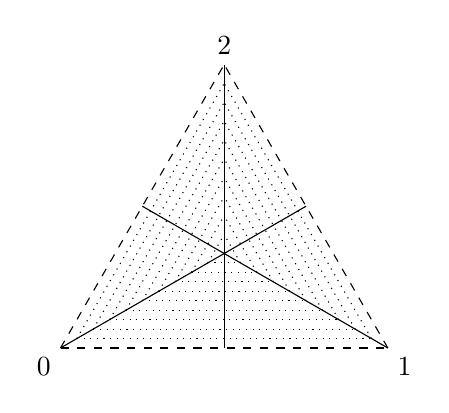
\begin{tikzpicture}[scale=0.8]
% Vertices of a triangle
\coordinate (2) at (90:3cm);
\coordinate (0) at (210:3cm);
\coordinate (1) at (-30:3cm);

% Nodes to mark vertices of a triangle
\node [above] at (2) {2};
\node [below left] at (0) {0};
\node [below right] at (1) {1};

% Draw line between the vertices 0,1 and 2 and name the midpoints
\draw [dashed] (0.north east)--(2.south) coordinate[midway](02);
\draw [dashed] (0.north east)--(1.north west) coordinate[midway](01);
\draw [dashed] (1.north west)--(2.south) coordinate[midway](12);

% Barycenter, could also be found by means of the intersection library of tikz
\coordinate (012) at (barycentric cs:0=1,1=1,2=1);

% Subdivide the 2-simplex
\foreach \x in {(0),(01),(1),(12),(2),(02)}
	\draw (012)--\x;

% Illustrate the effect of desingularization
\foreach \x in {0,1}
	\foreach \y in {1,2}
		\foreach \s in {1,...,9}
			\draw [dotted] (barycentric cs:\x=\s/10,012=1-\s/10)--(barycentric cs:\y=\s/10,012=1-\s/10);

\end{tikzpicture}
\caption{Desingularizing the Kan subdivision of the $2$-simplex with collapsed boundary.}
\label{fig:ch2_Desing_singlysubd_2simpl}
\end{figure}

Before we prove \cref{prop:double_subdivision_sphere_low_dimension} in the case when $n=2$, we contemplate how to desingularize $Sd(\Delta [2]/\partial \Delta [2])$, which is a similar task, although slightly easier. We make use of the notion of enforcer from \cref{def:enforcer}.
\begin{example}\label{ex:desingularization_model_n-sphere_subdivided}
Consider the cocartesian square
\begin{equation}
\label{eq:first_diagram_ex_desingularization_model_n-sphere_subdivided}
\begin{gathered}
\xymatrix{
Sd(\partial \Delta [2]) \ar[d] \ar[r] & Sd(\Delta [0]) \ar[d] \\
Sd(\Delta [2]) \ar[r] & Sd\, X
}
\end{gathered}
\end{equation}
in $sSet$, where we have written $X=\Delta [2]/\partial \Delta [2]$ for brevity. We will prove that
\begin{equation}\label{eq:first_equation_desingularization_model_n-sphere_subdivided}
DSd\, X\cong \Delta [1].
\end{equation}
In \cref{fig:ch2_Desing_singlysubd_2simpl}, we illustrate the effect of desingularizing $Sd\, X$. This illustration indicates the idea of the proof and is helpful in bookkeeping. The dashed line segments that are part of the boundary are meant to indicate that the boundary has been collapsed in order to form $\Delta [2]/\partial \Delta [2]$. The dotted line segments are meant to illustrate how identifications arise when desingularizing.

The simplicial set $Sd\, X$ is generated by six (non-degenerate) $2$-simplices as $Sd(\Delta [2])$ is generated by six non-degenerate $2$-simplices and as
\[Sd(\Delta [2])\to Sd\, X\]
is degreewise surjective. We will name these six generators. Let the simplex $y_1$ be the image under
\[B(\Delta [2])\cong Sd(\Delta [2])\to Sd\, X\]
of the simplex $\{0<01<012\}$. Furthermore, let $y_2$ be the image of the next non-degenerate $2$-simplex $\{1<01<012\}$ as we move counterclockwise in \cref{fig:ch2_Desing_singlysubd_2simpl} and so on up to and including $j=6$. Thus the set
\[\{y_j\} _{j\in J},\, J=\{ 1,\dots ,6\}\]
generates $Sd\, X$.

The simplicial set $Sd(\Delta [2])$ has seven $0$-simplices that correspond to the seven elements of $\Delta [2]^\sharp$. The six $0$-simplices on the boundary $Sd(\partial \Delta [2])$ are identified with each other when $Sd\, X$ is formed from $Sd(\Delta [2])$. However, the $0$-simplex $012$ is not identified with these. Write $z_j=\eta _{Sd\, X}(y_j)$ for each $j\in J$. Each of the $2$-simplices $y_j$, $j\in J$, is such that the vertices $y_j\varepsilon _0$ and $y_j\varepsilon _1$ are on the boundary and that $y_j\varepsilon _2$ is equal to $012$. Thus we see that each of the simplices $y_j$, $j\in J$, has the elementary degeneracy operator
\[\rho _{y_j}=\sigma _0\]
as its enforcer. Let $\rho$ denote this common enforcer.

For each $j\in J$, write $z_j=\eta _{Sd\, X}(y_j)$. From \cref{prop:role_of_enforcers}, we have the commutative square
\begin{equation}
\label{eq:second_diagram_ex_desingularization_model_n-sphere_subdivided}
\begin{gathered}
\xymatrix{
\bigsqcup _{j\in J}\Delta [2] \ar[d]_{\vee _{j\in J}(\bar{y} _j)} \ar[rr]^{\sqcup _{j\in J}(\rho )} && \bigsqcup _{j\in J}\Delta [1] \ar[d]^{\vee _{j\in J}(\bar{w} _j)} \\
Sd\, X \ar[rr]_{\eta _{Sd\, X}} && UDSd\, X
}
\end{gathered}
\end{equation}
in $sSet$, where $w_j$ is the canonical degeneracy of the non-degenerate part of $z_j$, $j\in J$.  In this case, the simplices $w_j$, $j\in J$, are embedded and therefore non-degenerate. This way we see how the simplices $z_j$, $j\in J$, are degenerate.

Because the simplices $z_j$, $j\in J$, are all degenerate it follows that $DSd\, X$ is generated by the images under $\eta _{Sd\, X}$ of the six embedded $1$-simplices of $Sd\, X$. We will argue that all of these images are equal.

Pick a $j\in J$. Two of the six embedded $1$-simplices of $Sd\, X$ are the faces $y_j\delta _1$ and $y_j\delta _0$ of $y_j$. Because $\delta _1$ and $\delta _0$ are both sections of $\rho$, we get that
\begin{displaymath}
\begin{array}{rclclcl}
z_j\delta _1 & = & (w_j\rho )\delta _1 & = & w_j(\rho \delta _1) & = & w_j \\
z_j\delta _0 & = & (w_j\rho )\delta _0 & = & w_j(\rho \delta _0) & = & w_j.
\end{array}
\end{displaymath}
Thus it follows that the image under $\eta _{Sd\, X}$ of each of the faces $y_j\delta _1$ and $y_j\delta _0$ is equal to $w_j$. Let us express this with $y_j\delta _1\sim y_j\delta _0$ for each $j\in J$.

By moving counterclockwise in \cref{fig:ch2_Desing_singlysubd_2simpl}, we get that
\begin{displaymath}
\begin{array}{rclcl}
y_1\delta _0 & = & y_2\delta _0 & \sim & y_2\delta _1 \\
y_2\delta _1 & = & y_3\delta _1 & \sim & y_3\delta _0 \\
y_3\delta _0 & = & y_4\delta _0 & \sim & y_4\delta _1 \\
y_4\delta _1 & = & y_5\delta _1 & \sim & y_5\delta _0 \\
y_5\delta _0 & = & y_6\delta _0 & \sim & y_6\delta _1.
\end{array}
\end{displaymath}
This shows that
\[w_1=w_2=\cdots =w_6,\]
implying that (\ref{eq:first_equation_desingularization_model_n-sphere_subdivided}) holds.
\end{example}
\noindent To complete \cref{tab:Desing_spherical_mod}, the only remaining case is when $k=2$ and $n=2$.

Note that the functor $BSd$ replaces a simplicial set with an ordered simplicial complex of the same homotopy type \cite[Ex.~3--8, pp.~219--220]{FP90}. To conjecture the homotopical content of the claim of \cref{prop:double_subdivision_sphere_low_dimension} one uses the sort of intuition that comes from knowledge of regular neighborhood theory, as explained in \cite[§3]{RS72} or \cite[§II]{Hu69}. For example, the reason that collapsing the boundary of $Sd^k(\Delta [2])$ in the category $nsSet$ is an operation that preserves the homotopy type in the case when $k=2$, but not in the case when $k=1$ is indicated and illustrated in a remark in \cite[p.~51]{Hu69}. It turns out that the double subdivision creates a sufficiently nice neighborhood around the boundary. \cref{fig:ch2_Desing_doublysubd_2simpl}, which is used for bookkeeping in the proof of \cref{prop:double_subdivision_sphere_low_dimension}, illustrates the phenomenon.  

% Takes advantage of barycentric coordinates and for loops. Can surely be more elegant.
\begin{figure}
\centering
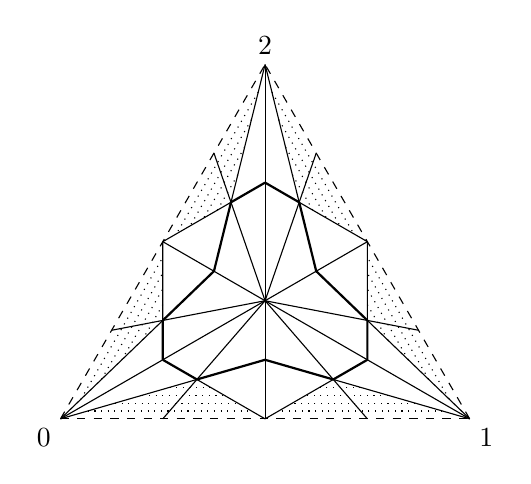
\begin{tikzpicture}

% Vertices of a triangle
\coordinate (2) at (90:3cm);
\coordinate (0) at (210:3cm);
\coordinate (1) at (-30:3cm);

% Nodes to mark vertices of a triangle
\node [above] at (2) {2};
\node [below left] at (0) {0};
\node [below right] at (1) {1};

% Draw line between the vertices 0,1 and 2 and name the midpoints
\draw [dashed] (0.north east)--(2.south) coordinate[midway](02);
\draw [dashed] (0.north east)--(1.north west) coordinate[midway](01);
\draw [dashed] (1.north west)--(2.south) coordinate[midway](12);

% Barycenter, could also be found by means of the intersection library of tikz
\coordinate (012) at (barycentric cs:0=1,1=1,2=1);

% Draws lines from vertices of original triangle to barycentre of original triangle and...
\draw (0.north east)--(012) coordinate[midway](0<012);
\draw (1.north west)--(012) coordinate[midway](1<012);
\draw (2.south)--(012) coordinate[midway](2<012);
\draw (01)--(012) coordinate[midway](01<012);
\draw (12)--(012) coordinate[midway](12<012);
\draw (02)--(012) coordinate[midway](02<012);

% Subdivide each of the six new 2-simplices. To highlight the structure of the desingularized simplicial set we make certain lines thicker
\coordinate (0<01<012) at (barycentric cs:0=1,01=1,012=1);
\coordinate (0<01) at (barycentric cs:0=0.5,01=0.5);
\foreach \x in {(0),(0<01),(01),(012)}
	\draw (0<01<012)--\x;
\foreach \x in {(0<012),(01<012)}
	\draw [thick] (0<01<012)--\x;

\coordinate (1<01<012) at (barycentric cs:1=1,01=1,012=1);
\coordinate (1<01) at (barycentric cs:1=0.5,01=0.5);
\foreach \x in {(1),(1<01),(01),(012)}
	\draw (1<01<012)--\x;
\foreach \x in {(01<012),(1<012)}
	\draw [thick] (1<01<012)--\x;

\coordinate (1<12<012) at (barycentric cs:1=1,12=1,012=1);
\coordinate (1<12) at (barycentric cs:1=0.5,12=0.5);
\foreach \x in {(1),(1<12),(12),(012)}
	\draw (1<12<012)--\x;
\foreach \x in {(12<012),(1<012)}
	\draw [thick] (1<12<012)--\x;

\coordinate (2<12<012) at (barycentric cs:2=1,12=1,012=1);
\coordinate (2<12) at (barycentric cs:2=0.5,12=0.5);
\foreach \x in {(2),(2<12),(12),(012)}
	\draw (2<12<012)--\x;
\foreach \x in {(12<012),(2<012)}
	\draw [thick] (2<12<012)--\x;
	
\coordinate (2<02<012) at (barycentric cs:2=1,02=1,012=1);
\coordinate (2<02) at (barycentric cs:2=0.5,02=0.5);
\foreach \x in {(2),(2<02),(02),(012)}
	\draw (2<02<012)--\x;
\foreach \x in {(02<012),(2<012)}
	\draw [thick] (2<02<012)--\x;
	
\coordinate (0<02<012) at (barycentric cs:0=1,02=1,012=1);
\coordinate (0<02) at (barycentric cs:0=0.5,02=0.5);
\foreach \x in {(0),(0<02),(02),(012)}
	\draw (0<02<012)--\x;
\foreach \x in {(02<012),(0<012)}
	\draw [thick] (0<02<012)--\x;

% Effect of desingularizing doubly subdivided 2-simplex with collapsed boundary. We make these lines dotted.
\foreach \x in {0.2,0.4,0.6,0.8}
	\draw [dotted] (barycentric cs:0=\x,0<01<012=1-\x)--(barycentric cs:01=\x,0<01<012=1-\x);

\foreach \x in {0.2,0.4,0.6,0.8}
	\draw [dotted] (barycentric cs:1=\x,1<01<012=1-\x)--(barycentric cs:01=\x,1<01<012=1-\x);

\foreach \x in {0.2,0.4,0.6,0.8}
	\draw [dotted] (barycentric cs:1=\x,1<12<012=1-\x)--(barycentric cs:12=\x,1<12<012=1-\x);

\foreach \x in {0.2,0.4,0.6,0.8}
	\draw [dotted] (barycentric cs:2=\x,2<12<012=1-\x)--(barycentric cs:12=\x,2<12<012=1-\x);

\foreach \x in {0.2,0.4,0.6,0.8}
	\draw [dotted] (barycentric cs:2=\x,2<02<012=1-\x)--(barycentric cs:02=\x,2<02<012=1-\x);

\foreach \x in {0.2,0.4,0.6,0.8}
	\draw [dotted] (barycentric cs:0=\x,0<02<012=1-\x)--(barycentric cs:02=\x,0<02<012=1-\x);
\end{tikzpicture}
\caption{Desingularizing the double Kan subdivision of the standard $2$-simplex with collapsed boundary.}
\label{fig:ch2_Desing_doublysubd_2simpl}
\end{figure}

We are ready to prove the proposition. The method is similar to that of \cref{ex:desingularization_model_n-sphere_subdivided}.
\begin{proof}[Proof of \cref{prop:double_subdivision_sphere_low_dimension}.]
We will argue that
\begin{equation}
\label{eq:first_expression_proof_of_prop_double_subdivision_sphere_low_dimension}
DSd^2\, X\cong S(12-gon)
\end{equation}
where $X=\Delta [2]/\partial \Delta [2]$. By this, we mean that $DSd^2\, X$ is the suspension of a $12$-gon, which is what $BSd\, X$ is. As the cases when $n=0$ and $n=1$ were taken care of by \cref{ex:all_subdivisions_sphere_dim_zero_coincidence_dim_one} and \cref{ex:double_subdivision_sphere_dim_one}, respectively, the argument below finishes the proof.

To study $DSd^2\, X$ is to study the diagram that we get by applying $Sd$ to (\ref{eq:first_diagram_ex_desingularization_model_n-sphere_subdivided}). For an illustration of the formation of $DSd^2\, X$ from $Sd^2\, X$, see \cref{fig:ch2_Desing_doublysubd_2simpl}. We use the same conventions as in \cref{fig:ch2_Desing_singlysubd_2simpl} and one additional convention. Namely, there are exactly twelve line segments that are thicker than the others. These form the $12$-gon we mentioned. The simplicial set $BSd\, X$ is the nerve of the poset
\begin{equation}
\label{eq:first_diagram_proof_prop_double_subdivision_sphere_low_dimension}
\begin{gathered}
\xymatrix@=0.6em{
&&&&&& [012] \\
\\
\\
&&&&&& \bullet \ar@{..>}[lllld] \ar@{<-}[uuu] \ar@/^0.3pc/@{<..}[ddddddddd] \ar@{..>}[drrrr] \\
&& \bullet \ar@{<..}[ddddddddrrrr] \ar@{<-}[uuuurrrr] &&&&&&&& \bullet \ar@{<..}[lllldddddddd] \ar@{<-}[lllluuuu] \\
&& \bullet \ar@{..>}[lld] \ar@{<..}[dddddddrrrr] \ar@{..>}[u] \ar@{<-}[uuuuurrrr] &&&&&&&& \bullet \ar@{<-}[lllluuuuu] \ar@{..>}[u] \ar@{<..}[llllddddddd] \ar@{..>}[drr] \\
\bullet \ar@{<..}[ddddddrrrrrr] \ar@{<-}[uuuuuurrrrrr] &&&&&&&&&&&& \bullet \ar@{<-}[lllllluuuuuu] \ar@{<..}[lllllldddddd] \\
\bullet \ar[u] \ar@{<-}[dddddrrrrrr] \ar@{<-}[uuuuuuurrrrrr] \ar[drr] &&&&&& \bullet \ar[lllld] \ar@/^0.3pc/@{<-}[uuuuuuu] \ar[drrrr] &&&&&& \bullet \ar[lld] \ar@{<-}[llllllddddd] \ar@{<-}[lllllluuuuuuu] \ar[u] \\
&& \bullet \ar@{<-}[ddddrrrr] \ar@{<-}[uuuuuuuurrrr] &&&&&&&& \bullet \ar@{<-}[lllluuuuuuuu] \ar@{<-}[lllldddd] \\
\\
\\
\\
&&&&&& [0] \ar[uuuuu]
}
\end{gathered}
\end{equation}
namely $Sd(X)^\sharp$. In (\ref{eq:first_diagram_proof_prop_double_subdivision_sphere_low_dimension}) we have drawn the $0$-simplex $012$ as the cone point at the top.

The cone point at the bottom, which we denote $[0]$, is the $0$-simplex that is the result of the identifications
\[0\sim 01\sim 1\sim 12\sim 2\sim 02.\]
These names arise in an intuitive manner from considering the poset $\Delta [2]^\sharp$ whose objects correspond to the $0$-simplices of
\[B(\Delta [2])\cong Sd(\Delta [2])\]
whose non-degenerate simplices in turn correspond to the $0$-simplices of
\[B^2(\Delta [2])\cong BSd(\Delta [2])\cong Sd^2(\Delta [2]).\]
For example, the object $0$ arises from $\varepsilon _0$ and $1$ from $\varepsilon _1$. Furthermore, the object $02$ arises from $\delta _1$. The objects of the poset $Sd(X)^\sharp$ that are not cone points are the non-degenerate $1$-simplices of $Sd\, X$, of which there are six, and the non-degenerate $2$-simplices, of which there are also six.

We proceed by naming the twelve non-embedded non-degenerate $2$-simplices of $Sd^2\, X$. First, we let $y_1$ be the image of
\[\{ \{0\} <\{0<01\} <\{0<01<012\} \}\]
under $Sd^2(\Delta [2])\to Sd^2\, X$. Next, we let $y_2$ be the image of the next $2$-simplex as we move counterclockwise in \cref{fig:ch2_Desing_doublysubd_2simpl} up to and including $j=12$. Write $J=\{ 1,\dots ,12\}$. Each of the simplices $y_j$, $j\in J$, has the elementary degeneracy operator
\[\rho _{y_j}=\sigma _0\]
as its enforcer. Let $\rho$ denote this common enforcer.

From \cref{prop:role_of_enforcers}, we have the cocartesian square
\begin{equation}
\label{eq:second_diagram_proof_prop_double_subdivision_sphere_low_dimension}
\begin{gathered}
\xymatrix{
\bigsqcup _{j\in J}\Delta [2] \ar[d]_{\vee _{j\in J}(\bar{y} _j)} \ar[rr]^{\sqcup _{j\in J}(\rho )} && \bigsqcup _{j\in J}\Delta [1] \ar[d] \\
Sd^2\, X \ar[rr] && Z
}
\end{gathered}
\end{equation}
in $sSet$. Let $z_j$, $j\in J$, be the image of $y_j$ under $Sd^2\, X\to Z$. Suppose $z_j=w_j\rho$ for some simplex $w_j$, $j\in J$. Then $w_j$ is embedded as $Sd^2\, X\to Z$ is injective in degree $0$.

The elementary face operators $\delta _1$ and $\delta _0$ are both sections of $\rho$, so we have
\begin{displaymath}
\begin{array}{rclclcl}
z_j\delta _1 & = & (w_j\rho )\delta _1 & = & w_j(\rho \delta _1) & = & w_j \\
z_j\delta _0 & = & (w_j\rho )\delta _0 & = & w_j(\rho \delta _0) & = & w_j.
\end{array}
\end{displaymath}
for each $j\in J$. It follows that the image under $Sd^2\, X\to Z$ of each of the faces $y_j\delta _1$ and $y_j\delta _0$ is equal to $w_j$. Let us express this with $y_j\delta _1\sim y_j\delta _0$.

Suppose $j\in J$ odd. Then
\[y_j\delta _1\sim y_j\delta _0=y_{j+1}\delta _0\sim y_{j+1}\delta _1.\]
Thus we observe that $w_j=w_{j+1}$. We get that $Z$ is non-singular by the bookkeeping performed with the aid of \cref{fig:ch2_Desing_doublysubd_2simpl}. From \cref{lem:pushout_along_enforcers_intermediate_desingularization}, it follows that the simplicial set $Z$ is the desingularization of $Sd^2\, X$. Moreover, the simplicial set $Z$ is the nerve of (\ref{eq:first_diagram_proof_prop_double_subdivision_sphere_low_dimension}). The naturality of $t_{Sd\, X}$ shows that it is an isomorphism.
\end{proof}


























\section{Iterative description}
\label{sec:description}

In the appendix of his PhD thesis, Gaunce Lewis Jr. \cite[p.~158]{Le78} makes explicit the least drastic way of transforming a $k$-space into a compactly generated space, which is (defined as) a space that is both a $k$-space and a weak Hausdorff space. Lewis describes an iterative process. At each stage of the process, two points are identified whenever it is impossible to separate them by (disjoint) open sets.

We will provide an iterative description of the process of forming $UDX$ from $X$ that is analogous to Lewis' method. In the least drastic way possible, we want to make a quotient of $X$ so that the vertices of any non-degenerate simplex are pairwise distinct. In other words, any non-degenerate simplex of $X$ whose vertices are not pairwise distinct, must be made degenerate. For this purpose, we will use the notion of enforcer from \cref{def:enforcer}.

In relation to \cref{thm:main_result_itdesing}, there is a systematic study of reflective subcategories provided by S. Baron \cite{Ba69}. First, $nsSet$ is epi-reflective as the map $X\to DX$ is epic in general. Second, Baron discusses the possibility of factoring the reflector through a unique intermediate category.

In the following way, we define a functor $J:sSet\to sSet$ together with a natural quotient map $X\to JX$ that $\eta _X$ factors through. The functor $J$ is thought of as a preferred first step towards making a simplicial set non-singular. We have taken the symbol $J$ because Lewis uses it to denote his analogous endofunctor of $k$-spaces.

Let $X$ be a simplicial set. Given a non-degenerate simplex $x$ of $X$, we let $n_x$ denote its degree. Recall the enforcer $\rho _x:[n_x]\to [m_x]$ of $x$ from \cref{def:enforcer}. We will construct a cobase change of
\[A=\bigsqcup _{x\in X^\sharp}\Delta [n_x]\xrightarrow{f=\sqcup _{x\in X^\sharp }(\rho _x)} \bigsqcup _{x\in X^\sharp}\Delta [m_x]=B\]
along
\[A\xrightarrow{g=\vee _{x\in X^\sharp }(\bar{x} )} X.\]
The latter map is degreewise surjective as $X^\sharp$ generates $X$.

For each integer $n\geq 0$, define a symmetric binary relation $R'_n$ on $X_n$ by letting $(x,x')\in X_n\times X_n$ be a member of a set $R'_n$ if there are $a,a'\in A_n$ such that
\begin{displaymath}
\begin{array}{rcl}
x & = & g(a) \\
x' & = & g(a') \\
f(a) & = & f(a').
\end{array}
\end{displaymath}
The binary relation $R'_n$, $n\geq 0$, is reflexive as $g$ is degreewise surjective.

Let $R_n$ be the equivalence relation generated by $R'_n$, for each $n$. It follows immediately that the equivalence relations $R_n$, $n\geq 0$, satisfy the condition that the diagrams (\ref{eq:first_diagram_proof_lem_desing_unique_factorization_through_unit}) commute. This implies that we can form the quotient
\[JX=X/R.\]
Thus we obtain the cocartesian square
\begin{displaymath}
 \xymatrix{
 \bigsqcup _{x\in X^\sharp}\Delta [n_x] \ar[d]_{\vee _{x\in X^\sharp }(\bar{x} )} \ar[rr]^{\sqcup _{x\in X^\sharp }(\rho _x)} && \bigsqcup _{x\in X^\sharp}\Delta [m_x] \ar[d] \\
 X \ar[rr] && JX
 }
\end{displaymath}
in $sSet$. By \cref{lem:pushout_along_enforcers_intermediate_desingularization}, it gives rise to a commutative triangle
\begin{equation}
\label{eq:first_diagram_description_iterative}
\begin{gathered}
\xymatrix{
X \ar[dr]_{\eta _X} \ar[rr] && JX \ar[ld] \\
& UDX
}
\end{gathered}
\end{equation}
that factors the unit $\eta _X$ through a quotient map $X\to JX$, which is the identity in the case when $X$ is already non-singular.

For the purposes of making an iterative description of desingularization, the notation above is suitable. However, the construction $JX$ deserves its own name.
\begin{definition}\label{def:enforced_collapse}
Let $X$ be a simplicial set. The map $X\to JX$ is the \textbf{enforced collapse} of $X$.
\end{definition}
\noindent Outside of the context of the iteration process below we may choose to use the following symbol
\begin{notation}
Let $X$ be a simplicial set. Let
\[Cen(X)=JX\]
denote the enforced collapse of $X$.
\end{notation}
\noindent Note that the enforced collapse need not be non-singular, as \cref{ex:infinitely_many_enforced_collapses_needed} shows.
\begin{example}\label{ex:infinitely_many_enforced_collapses_needed}
Consider the $2$-dimensional simplicial set depicted in \cref{fig:ch2_finite_number_of_enforced_collapses_not_enough}. Identify the two $0$-simplices $v$ and $w$. The result can be constructed thus.

Let
\[\mathbb{N} =\{ 1,2,\dots \}\]
and
\[\mathbb{N} _0=\{ 0,1,2,\dots \} .\]
Next, for each $n\in 2\mathbb{N}$, let $B_n=\Delta [2]$. For each $n\in \mathbb{N} _0$, let $A_n=\Delta [1]$. Furthermore, let $C_0=\Delta [1]/\partial \Delta [1]$. Finally, for each $n\in \mathbb{N}$, let $C_n=\Delta [1]$.

Take the pushout $X$ in $sSet$ of
\begin{equation}
\label{eq:first_diagram_ex_infinitely_many_enforced_collapses_needed}
\begin{gathered}
\xymatrix{
\bigsqcup _{n\in \mathbb{N} _0}A_n \ar[d] \ar[r] & \bigsqcup _{n\in 2\mathbb{N} _0}C_n \\
\bigsqcup _{n\in 2\mathbb{N} }B_n
}
\end{gathered}
\end{equation}
where the maps are defined as follows. Let $X$ denote the pushout.

Suppose $n\in \mathbb{N} _0$. In the case when $n\equiv 0\; (mod\, 4)$, we let $A_n\to B_{n+2}$ be the map induced by $\delta _1$ and we let $A_{n+1}\to B_{n+2}$ be the map induced by $\delta _2$. In the case when $n\equiv 2\; (mod\, 4)$, we let $A_n\to B_{n+2}$ be the map induced by $\delta _1$ and we let $A_{n+1}\to B_{n+2}$ be the map induced by $\delta _0$. These maps give rise to the map
\[\bigsqcup _{n\in \mathbb{N} _0}A_n\to \bigsqcup _{n\in 2\mathbb{N} }B_n\]
in (\ref{eq:first_diagram_ex_infinitely_many_enforced_collapses_needed}).

Let $A_0\to C_0$ be the canonical map. Suppose $n\in \mathbb{N} _0$ odd. Then we let $A_n\to C_{n+1}$ and $A_{n+1}\to C_{n+1}$ be the identity $\Delta [1]\to \Delta [1]$. These maps give rise to the map
\[\bigsqcup _{n\in \mathbb{N} _0}A_n\to \bigsqcup _{n\in 2\mathbb{N} _0}C_n\]
in (\ref{eq:first_diagram_ex_infinitely_many_enforced_collapses_needed}).

If $Cen^k$ denotes the $k$-fold iteration of the enforced collapse for $k$ a non-negative integer, then $Cen^k(X)$ is singular for every $k$.
\end{example}
\noindent \cref{ex:infinitely_many_enforced_collapses_needed} shows that one might need an infinite number of enforced collapses in order to make a simplicial set non-singular.

\begin{figure}
\centering
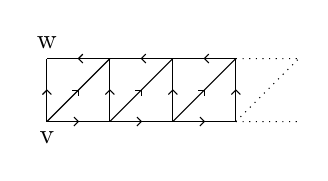
\begin{tikzpicture}[scale=0.4]

% $0$-simplices coordinates
\coordinate (0) at (-5,-1);
\coordinate (2) at (-3,-1);
\coordinate (4) at (-1,-1);
\coordinate (6) at (1,-1);

\coordinate (1) at (-5,1);
\coordinate (3) at (-3,1);
\coordinate (5) at (-1,1);
\coordinate (7) at (1,1);


% Nodes to aid in the drawing process
\node [below] at (0) {v};
% \node [below] at (2) {2};
% \node [below] at (4) {4};
% \node [below] at (6) {6};

\node [above] at (1) {w};
% \node [above] at (3) {3};
% \node [above] at (5) {5};
% \node [above] at (7) {7};


% $1$-simplices drawn
\draw (0.north)--(1.south) coordinate[midway](01);
\draw (2.north)--(3.south) coordinate[midway](23);
\draw (4.north)--(5.south) coordinate[midway](45);
\draw (6.north)--(7.south) coordinate[midway](67);

\draw (0.north)--(3.south) coordinate[midway](03);
\draw (2.north)--(5.south) coordinate[midway](25);
\draw (4.north)--(7.south) coordinate[midway](47);
\draw [dotted] (6.north)--(3,1);

\draw (0.north)--(2.north) coordinate[midway](02);
\draw (2.north)--(4.north) coordinate[midway](24);
\draw (4.north)--(6.north) coordinate[midway](46);
\draw [dotted] (6.north)--(3,-1);

\draw (1.south)--(3.south) coordinate[midway](13);
\draw (3.south)--(5.south) coordinate[midway](35);
\draw (5.south)--(7.south) coordinate[midway](57);
\draw [dotted] (7.south)--(3,1);

% Directions
\draw (01)--+(225:0.2cm);
\draw (01)--+(315:0.2cm);

\draw (23)--+(225:0.2cm);
\draw (23)--+(315:0.2cm);

\draw (45)--+(225:0.2cm);
\draw (45)--+(315:0.2cm);

\draw (67)--+(225:0.2cm);
\draw (67)--+(315:0.2cm);


\draw (02)--+(135:0.2cm);
\draw (02)--+(225:0.2cm);

\draw (24)--+(135:0.2cm);
\draw (24)--+(225:0.2cm);

\draw (46)--+(135:0.2cm);
\draw (46)--+(225:0.2cm);


\draw (13)--+(45:0.2cm);
\draw (13)--+(315:0.2cm);

\draw (35)--+(45:0.2cm);
\draw (35)--+(315:0.2cm);

\draw (57)--+(45:0.2cm);
\draw (57)--+(315:0.2cm);


\draw (03)--+(180:0.2cm);
\draw (03)--+(270:0.2cm);

\draw (25)--+(180:0.2cm);
\draw (25)--+(270:0.2cm);

\draw (47)--+(180:0.2cm);
\draw (47)--+(270:0.2cm);
\end{tikzpicture}
\caption{Simplicial set such that every finite iteration of enforced collapses is singular.}
\label{fig:ch2_finite_number_of_enforced_collapses_not_enough}
\end{figure}

We point out the following, which is not really part of the storyline.
\begin{remark}\label{rem:description_iterative}
The map $\vee _{x\in X^\sharp }(\bar{x} )$ is degreewise surjective because $X^\sharp$ generates $X$. In this way, the construction of the functor $J$ is less arbitrary than the setting in \cref{lem:pushout_along_enforcers_intermediate_desingularization}.

One can, however, replace $X^\sharp$ with a subset and still construct symmetric binary relations $R'_n$, $n\geq 0$, the same way. Each of them is reflexive if and only if the subset generates $X$. We can in either case choose a quotient map as the cobase change of $\sqcup _{x\in X^\sharp }(\rho _x)$ along $\vee _{x\in X^\sharp }(\bar{x} )$.

For example, in the proof of \cref{prop:double_subdivision_sphere_low_dimension}, or more specifically the diagram (\ref{eq:second_diagram_proof_prop_double_subdivision_sphere_low_dimension}), we did choose a suitable subset of the set of non-degenerate simplices to perform a desingularization.
\end{remark}
\noindent \cref{rem:description_iterative} might be useful in some cases as suggested by the proof of \cref{prop:double_subdivision_sphere_low_dimension}.

To define $J$ on morphisms $f:X\to Y$ we need a diagram of the form
\begin{equation}
\label{eq:second_diagram_description_iterative}
\begin{gathered}
 \xymatrix{
 X \ar[d]_f & \bigsqcup _{x\in X^\sharp}\Delta [n_x] \ar[l] \ar[d] \ar[r] & \bigsqcup _{x\in X^\sharp}\Delta [m_x] \ar@{-->}[d] \\
 Y & \bigsqcup _{y\in Y^\sharp}\Delta [n_y] \ar[l] \ar[r] & \bigsqcup _{y\in Y^\sharp}\Delta [m_y]
 }
\end{gathered}
\end{equation}
in which an obvious choice of middle vertical map is $f(x)^\flat$ for each index $x\in X^\sharp$. Here, we write $f(x)=f(x)^\sharp f(x)^\flat$ by means of the Eilenberg-Zilber lemma.

There is at most one dashed map that makes the square
\begin{equation}
\label{eq:third_diagram_description_iterative}
\begin{gathered}
 \xymatrix{
 [n_x] \ar[d]_{f(x)^\flat } \ar[r]^{\rho _x} & [m_x] \ar@{-->}[d] \\
 [n_{f(x)^\sharp }] \ar[r]_{\rho _{f(x)^\sharp }} & [m_{f(x)^\sharp }]
 }
\end{gathered}
\end{equation}
commute as $\rho _x$. We claim that if $\mu _x$ is a section of $\rho _x$, then
\[\rho _{f(x)\sharp }\circ f(x)^\flat \circ \mu _x\]
makes the square commute. This claim holds if
\begin{equation}\label{eq:first_equation_description_iterative}
\rho _{f(x)^\sharp }\circ f(x)^\flat (i)=\rho _{f(x)^\sharp }\circ f(x)^\flat (j)
\end{equation}
whenever
\begin{equation}\label{eq:second_equation_description_iterative}
\rho _x(i)=\rho _x(j).
\end{equation}
If the claim holds, then any other section of $\rho _x$ would yield the same functor $[k_x]\to [k_{f(x)^\sharp }]$. From dashed maps that makes the diagrams (\ref{eq:third_diagram_description_iterative}) commute, we get a dashed map that makes (\ref{eq:second_diagram_description_iterative}) commute. With it arises a map $J(f)$.

Now we argue that (\ref{eq:first_equation_description_iterative}) holds whenever (\ref{eq:second_equation_description_iterative}) does. The degeneracy operator $\rho _x$ corresponds to the equivalence relation on $[n_x]$ that is generated by the reflexive binary relation $\approx$ that is defined in \cref{sec:calculations}. Hence, our claim will follow if $i\approx k$ implies that
\begin{equation}\label{eq:third_equation_description_iterative}
\rho _{f(x)^\sharp }\circ f(x)^\flat (i)=\rho _{f(x)^\sharp }\circ f(x)^\flat (k)
\end{equation}
holds.

Suppose $x\varepsilon _i=x\varepsilon _j$. This implies $f(x)\varepsilon _i=f(x)\varepsilon _j$, which can be rewritten as
\[f(x)^\sharp f(x)^\flat \varepsilon _i=f(x)^\sharp f(x)^\flat \varepsilon _j,\]
which in turn can be rewritten as
\[f(x)^\sharp \varepsilon _{f(x)^\flat (i)}=f(x)^\sharp \varepsilon _{f(x)^\flat (j)}.\]
By definition of $\rho _{f(x)^\sharp }$ it follows that
\[\rho _{f(x)^\sharp }(f(x)^\flat (i))=\rho _{f(x)^\sharp }(f(x)^\flat (j)).\]
Next, suppose $i\leq k\leq j$. In other words, we assume $i\approx k$. Degeneracy operators are order-preserving, so (\ref{eq:third_equation_description_iterative}) holds. This concludes our definition of $J(f)$.

It is clear that $J(id)=id$, for in the case $f=id$ we have that $f(x)^\flat =id$ and $\rho _x=\rho _{f(x)^\sharp }$. It follows that
\[J(g\circ f)=J(g)\circ J(f)\]
from the fact that the square
\begin{displaymath}
\xymatrix{
X \ar[d] \ar[r]^f & Y \ar[d] \\
JX \ar[r]_{J(f)} & JY
}
\end{displaymath}
commutes for each simplicial map $f:X\to Y$ combined with the fact that $X\to JX$ is degreewise surjective for each simplicial set $X$. Thus the construction $JX$ is functorial and the map $X\to JX$ is natural. Because $X\to JX$ is natural and degreewise surjective and because $\eta _X$ is natural, it follows that $JX\to UDX$ is natural.

The plan is to obtain a quotient of $X$ that is isomorphic to $UDX$ by applying $J$ successively. Moreover, we aim to establish \cref{thm:main_result_itdesing}. To arrange for the iteration, we refer to \cref{def:sequence_composition}. Let $f^{0,1}$ be the natural map
\[J^0X=X\to JX=J^1X.\]
Due to (\ref{eq:first_diagram_description_iterative}), we can assume that we for some ordinal $\gamma >1$ have defined a $\gamma$-sequence
\[T^{[0]}\Rightarrow \cdots \Rightarrow T^{[\beta ]}\Rightarrow T^{[\beta +1]}\Rightarrow \cdots\]
of commutative triangles
\begin{equation}
\label{eq:fourth_diagram_description_iterative}
\begin{gathered}
\xymatrix{
X \ar[dr]_{\eta _X} \ar[rr] && J^\beta X \ar[ld]^{p^\beta} \\
& UDX
}
\end{gathered}
\end{equation}
denoted $T^{[\beta ]}$ and natural transformations, in which the component
\[J^\alpha X\xrightarrow{f^{\alpha ,\beta }} J^\beta X\]
of $T^{[\alpha ]}\Rightarrow T^{[\beta ]}$ is a quotient map whenever $\alpha \leq \beta <\gamma$.

If $\gamma$ is a limit ordinal, then we take the colimit in the following way to define $J^\gamma X$. For each $n\geq 0$, let $R_n$ be the equivalence relation on $J^0X=X$ that consists of the elements $(x,y)\in X_n\times X_n$ such that there is some $\beta <\gamma$ with $f^{0,\beta }(x)=f^{0,\beta }(y)$. It is clear that the diagrams (\ref{eq:first_diagram_proof_lem_desing_unique_factorization_through_unit}) commute so that we obtain the quotient $J^\gamma X=X/R$ of $J^0X$. In this case, we automatically get a diagram $T^{[\gamma ]}$ that plays the role of (\ref{eq:fourth_diagram_description_iterative}).

Else if $\gamma =\beta +1$ is a successor of an ordinal $\beta$, then we simply define $J^{\beta +1}X$ by applying $J$ to $J^\beta X$. Consider the solid commutative diagram
\begin{equation}
\label{eq:fifth_diagram_description_iterative}
\begin{gathered}
\xymatrix{
X \ar[dd]_{id} \ar[dr]_{\eta _X} \ar[rr] && J^\beta X \ar[ld]^{p^\beta } \ar[dd]^{f^{\beta ,\beta +1}} \\
& UDX \ar[dd]_(.65){id} \\
X \ar[dr]_{\eta _X} \ar@{-}[r] & \ar[r] & J^{\beta +1}X \ar@{-->}[ld]^{p^{\beta +1}} \\
& UDX
}
\end{gathered}
\end{equation}
in which we have yet to define the dashed map $p^{\beta +1}$. By \cref{prop:role_of_enforcers}, we obtain the dashed map in the solid diagram
\begin{equation}
\label{eq:sixth_diagram_description_iterative}
\begin{gathered}
\xymatrix{
& \bigsqcup _{j\in (J^\beta X)^\sharp}\Delta [n_j] \ar[dd]_{\vee _{j\in (J^\beta X)^\sharp }(\bar{\jmath } )} \ar[rr]^{\sqcup _{j\in (J^\beta X)^\sharp }(\rho _j)} && \bigsqcup _{j\in (J^\beta X)^\sharp}\Delta [m_j] \ar[dd] \\
\\
X \ar[d]_\eta \ar[r]^{f^{0,\beta }} & J^\beta X \ar[ld]^(.45){p^\beta } \ar[d]^\eta \ar[rr]^{f^{\beta ,\beta +1}} && J^{\beta +1}X \ar@{-->}[lld] \ar[d]^\eta \\
UDX \ar[r]_(.45){UD(f^{0,\beta })} & UD(J^\beta X) \ar[rr]_{UD(f^{\beta ,\beta +1})} && UD(J^{\beta +1})
}
\end{gathered}
\end{equation}
in $sSet$, which commutes because $f^{0,\beta }$ is a quotient map and hence degreewise surjective.

The whole diagram (\ref{eq:sixth_diagram_description_iterative}) commutes because $f^{\beta ,\beta +1}$ is degreewise surjective. This implies that $UD(f^{0,\beta })$ and $UD(f^{\beta ,\beta +1})$ are isomorphisms. Hence, from (\ref{eq:sixth_diagram_description_iterative}) we obtain a canonical dashed map $p^{\beta +1}$ in (\ref{eq:fifth_diagram_description_iterative}) that makes the whole diagram commute, including the lower triangle.

We have finished the construction of a $\gamma$-sequence $T:\gamma \to sSet^{[2]}$ for each ordinal $\gamma$. By the design of these sequences, there is a canonical composition of each of them that is a quotient map.

Next, we verify that this iterative process does indeed come to a halt. The proof uses the following observation.
\begin{lemma}\label{lem:no_break_iterative_desingularization}
If $\beta$ is some ordinal and if some $x\in (J^\beta X)^\sharp$ is not embedded, then $f^{\beta ,\beta +1}(x)$ is a degenerate simplex in $J^{\beta +1}X$.
\end{lemma}
\begin{proof}
Consider the diagram
\begin{equation}
\label{eq:first_diagram_proof_lem_no_break_iterative_desingularization}
\begin{gathered}
\xymatrix@=0.7em{
\Delta [n_x] \ar[dd] \ar[rr]^{\rho _x} && \Delta [m_x] \ar@/_1.9pc/[lddd] \ar[dd] \\
\\
\bigsqcup _{j\in (J^\beta X)^\sharp }\Delta [n_j] \ar[dd]_{\vee _{j\in (J^\beta X)^\sharp }{(\bar{\jmath } )}} \ar@{-}[r] & \ar[r] & \bigsqcup _{j\in (J^\beta X)^\sharp }\Delta [m_j] \ar[dd] \\
& Y \ar@{-->}[dr] \\
J^\beta X \ar[ur] \ar[rr]_{f^{\beta ,\beta +1}} && J^{\beta +1}X
}
\end{gathered}
\end{equation}
where we take the pushout
\[Y=J^\beta X\sqcup _{\Delta [n_x]}\Delta [m_x].\]
The quotient map $f^{\beta ,\beta +1}X$ factors through the canonical map $J^\beta X\to Y$. The map $Y\to J^{\beta +1}X$ is then also degreewise surjective. To say that $x$ is not embedded is the same as saying that its vertices are not pairwise distinct, so $\rho _x$ is a proper degeneracy operator. Thus we see that
\[\Delta [n_x]\xrightarrow{\bar{x} } J^\beta X\to Y\]
is the representing map of a degenerate simplex. To precompose this representing map with $Y\to J^{\beta +1}X$ yields the map $f^{\beta ,\beta +1}\circ \bar{x}$, as we see from (\ref{eq:first_diagram_proof_lem_no_break_iterative_desingularization}). It follows that $f^{\beta ,\beta +1}(x)$ is degenerate.
\end{proof}
\begin{proposition}\label{prop:iterative_desingularization_halts}
Let $X$ be a simplicial set. There is an ordinal $\lambda$ such that $J^\lambda X$ is non-singular.
\end{proposition}
\begin{corollary}\label{cor:iterative_desingularization_halts}
Let $X$ be a simplicial set. There is an ordinal $\lambda$ such that the map
\[p^\lambda :J^\lambda X\xrightarrow{\cong } UDX\]
is an isomorphism.
\end{corollary}
\begin{proof}[Proof of \cref{cor:iterative_desingularization_halts}.]
Use \cref{prop:iterative_desingularization_halts} to choose an ordinal $\kappa$ such that $J^\kappa X$ is non-singular.

According to \cref{lem:pushout_along_enforcers_intermediate_desingularization}, the canonical map $J^{\kappa +1}X\xrightarrow{\cong } UD(J^\kappa X)$ is an isomorphism as $J^{\kappa +1}X$ is non-singular, which is in turn because $f^{\kappa ,\kappa +1}$ is the identity. Recall the successor ordinal step from the construction of $T$ and replace $\beta$ with $\kappa$ in the diagram (\ref{eq:sixth_diagram_description_iterative}).

As $f^{\kappa ,\kappa +1}$ is the identity, it follows that the isomorphism above is in fact equal to $\eta _{J^\kappa X}$. The map $J^{\kappa +1}X\to UDX$ is by design equal to the composite
\[J^{\kappa +1}X=J^\kappa X\xrightarrow{\eta _{J^\kappa X}} UD(J^\kappa X)\to UDX.\]
The first half $\eta _{J^\kappa X}$ of the composite above is an isomorphism by the choice of $\kappa$ and the second half is the inverse of
\[UD(f^{0,\kappa }):UDX\to UD(J^\kappa X)\]
If we define $\lambda =\kappa +1$, then the proof is finished.
\end{proof}
\begin{proof}[Proof of \cref{prop:iterative_desingularization_halts}.]
The idea of the proof is that we can index the simplicial sets $J^\beta X$ that are singular by a certain subset of the non-degenerate simplices of $X$.

If $J^0X=X$ is already non-singular, then we can let $\lambda =0$. Else if $X$ is singular, then we choose a non-embedded non-degenerate simplex $x^0$ of $X$. Suppose $\gamma >0$ is such that we for all $\beta$ with $\beta <\gamma$ have defined $x^\beta$ with $x^\alpha \neq x^\beta$ if $\alpha <\beta <\gamma$.

If $J^\gamma X$ is non-singular, then we define $\lambda =\gamma$. Else if $J^\gamma X$ is singular, then we choose a simplex $x^\gamma$ of $X$ such that $f^{0,\gamma }(x^\gamma )$ is a non-embedded non-degenerate simplex. Suppose $\beta$ an ordinal with $\beta <\gamma$. From the commutative diagram
\begin{equation}
\label{eq:first_diagram_proof_prop_iterative_desingularization_halts}
\begin{gathered}
 \xymatrix{
 X \ar[dr]_{f^{0,\beta }} \ar[rr]^{f^{0,\gamma }} && J^\gamma X \\
 & J^\beta X \ar[ur]^{f^{\beta ,\gamma }} \ar[rr]_{f^{\beta ,\beta +1}} && J^{\beta +1}X \ar[lu]_{f^{\beta +1,\gamma }}
 }
 \end{gathered}
\end{equation}
we will conclude that
\begin{equation}\label{eq:first_equation_proof_prop_iterative_desingularization_halts}
x^\beta \neq x^\gamma
\end{equation}
in the following way.

Define
\begin{displaymath}
\begin{array}{rcl}
y & = & f^{0,\beta }( x^\beta) \\
y' & = & f^{\beta ,\beta +1}(y) \\

\end{array}
\end{displaymath}
As $y'$ is degenerate by \cref{lem:no_break_iterative_desingularization}, it follows that $f^{\beta +1,\gamma }(y')$ is degenerate. Because the diagram (\ref{eq:first_diagram_proof_prop_iterative_desingularization_halts}) commutes, this simplex is equal to
\[f^{\beta +1,\gamma }(y')=f^{\beta ,\gamma }(y)=f^{0,\gamma }(x^\beta ).\]
On the other hand, the simplex $f^{0,\gamma }(x^\gamma )$ is non-degenerate, so, as announced, it follows that (\ref{eq:first_equation_proof_prop_iterative_desingularization_halts}) holds.

Let $\lambda$ be a cardinal that is strictly greater than the cardinality of $X^\sharp$. Define $S$ as the set consisting of those $x^\beta$ with $\beta \leq \lambda$. This is a subset of $X^\sharp$. Then we can consider the injective function $S\to \lambda +1$ defined by $x^\beta \mapsto \beta$. If $\alpha <\beta$, then $x^\alpha$ is defined if $x^\beta$ is. In other words, $\alpha$ is in the image of $S\to \lambda +1$ if $\beta$ is.

By the choice of $\lambda$, there does not exist a surjective extension
\begin{displaymath}
\xymatrix{
S \ar[dd] \ar[dr] \\
& \lambda +1 \\
X^\sharp \ar@{-->>}[ur]_\nexists
}
\end{displaymath}
of $S\to \lambda +1$ to $X^\sharp$. Therefore, the function $S\to \lambda +1$ cannot possibly be surjective. Hence, the element $\lambda$ is not in the image of the latter function. By the definition of $S$, it follows that $x^\lambda$ is not defined. This implies that the set $S$ contains every element in $X^\sharp$ with a designation $x^\beta$. This shows that $J^\lambda X$ is non-singular.
\end{proof}
\begin{proof}[Proof of \cref{thm:main_result_itdesing}.]
Use \cref{cor:iterative_desingularization_halts} to choose an ordinal $\lambda$ such that $p^\lambda$ is an isomorphism. Take the corresponding $\lambda$-sequence $T$ of triangles (\ref{eq:fourth_diagram_description_iterative}) from the family of sequences constructed above. The map $f^{0,\lambda }$ is the composition of the $\gamma$-sequence
\[J^0X\xrightarrow{f^{0,1}} \cdots \to J^\beta X\xrightarrow{f^{\beta ,\beta +1}} \cdots\]
by the design of $J^{\lambda +1}$. Because $p^\lambda$ is an isomorphism, the commutative triangle $T^{[\lambda ]}$ identifies $f^{0,\lambda }$ with $\eta _X$.
\end{proof}






    
\chapter{Exponentials of non-singular simplicial sets}
\label{ch:exponentials}


\begin{abstract}
\noindent A simplicial set is \textbf{non-singular} if the representing maps of its non-degenerate simplices are degreewise injective. The category of simplicial sets has a \textbf{simplicial mapping set} $X^K$ whose set of $n$-simplices are the simplicial maps $\Delta [n]\times K\to X$. We prove that $X^K$ is non-singular whenever $X$ is non-singular.
\end{abstract}
\section{Introduction}
\label{sec:intro_exp}

There are times when one would like to know whether a category behaves similarly, in some sense, to the category of sets and functions. As an example, for homotopy-theoretical purpose the author would like to know whether the endofunctor $-\times \Delta [1]$ of non-singular simplicial sets preserves colimits. Here, $\Delta [1]$ denotes the standard $1$-simplex.

Let $sSet$ denote the category of simplicial sets. The full subcategory $nsSet$ whose objects are the non-singular simplicial sets sits strictly between $sSet$ and the category of ordered simplicial complexes. Despite the fact that non-singular simplicial sets have a natural PL structure \cite[p.~126--127]{WJR13} they almost never appear in the literature, though they do play a role in the book Spaces of PL Manifolds and Categories of Simple Maps by Waldhausen, Jahren and Rognes \cite{WJR13}.

The endofunctor $(-)^K:sSet\to sSet$ is designed so that the Yoneda lemma makes it right adjoint to $-\times K$. Our main result is the following.
\begin{theorem}\label{thm:arbitrary_exponent}
Let $K$ be some simplicial set. Then $X^K$ is non-singular whenever $X$ is.
\end{theorem}
\noindent Part of the author's interest in this result comes from the case when $K$ non-singular. Then the restriction of $(-)^K$ to $nsSet$ corestricts to an endofunctor of non-singular simplicial sets. Moreover, $(-)^K$ viewed as a functor $nsSet\to nsSet$ is right adjoint to the endofunctor $-\times K$ of $nsSet$. This means that we can derive the following consequence of \cref{thm:arbitrary_exponent}.
\begin{corollary}\label{cor:take_product_cocontinous_endofunctor_non-singular}
Taking the product $-\times K:nsSet\to nsSet$ with a non-singular simplicial set $K$ preserves colimits.
\end{corollary}
\noindent In particular, taking the product $-\times \Delta [1]$ with an interval is a cocontinous endofunctor of non-singular simplicial sets.

The case of the interval is not only of practicle concern, but it is also the theoretical focus of this article as it is not hard to argue that \cref{thm:arbitrary_exponent} follows from the following result.
\begin{proposition}\label{prop:standard_1_simplex_as_exponent}
The simplicial set $X^{\Delta [1]}$ is non-singular whenever $X$ is.
\end{proposition}
\noindent The proof of the latter result is the subject of \cref{sec:prism}, whereas \cref{thm:arbitrary_exponent} is derived from \cref{prop:standard_1_simplex_as_exponent} in \cref{sec:arbexp}.

In \cref{sec:app}, we will discuss applications of \cref{thm:arbitrary_exponent} beyond \cref{cor:take_product_cocontinous_endofunctor_non-singular}. We explain how \cref{thm:arbitrary_exponent} follows from \cref{prop:standard_1_simplex_as_exponent} in \cref{sec:arbexp}. Finally, the case of the interval is discussed \cref{sec:prism}.






\section{Applications}
\label{sec:app}

The inclusion $U:nsSet\to sSet$ admits a left adjoint functor called desingularization \cite[Rem.~2.2.12.,~p.~39]{WJR13}, which is denoted $D$. Note that the unit
\[\eta _X:X\to UDX\]
is degreewise surjective and that desingularization has the universal property that any simplicial map $f:X\to Y$ whose target $Y$ is non-singular factors through the unit by a unique map $UDX\to Y$.

In general, we say that a full subcategory of some category is a \textbf{reflective subcategory} if the inclusion admits a left adjoint, which is then referred to as a \textbf{reflector}. Thus $nsSet$ is a reflective subcategory of $sSet$. Note that the word reflective is not quite standard terminology. For example, Mac Lane \cite[§IV.3]{ML98} Adámek and Rosický \cite[p.~1306]{AR15} do not include fullness as an assumption in their definition, although some other authors do. \cref{prop:standard_1_simplex_as_exponent} and its generalization \cref{thm:arbitrary_exponent} has a noteworthy application and a couple of consequences.

\cref{thm:main_homotopy_theory} establishes a model structure on $nsSet$ that is right-induced a la Thomason \cite{Th80} from $sSet$ equipped with the standard model structure due to Quillen \cite{Qu67}. Moreover, the theorem says that $(D,U)$ is a Quillen equivalence. \cref{prop:standard_1_simplex_as_exponent} is used as a technical ingredient in the proof of \cref{thm:main_homotopy_theory}.

Another way to state \cref{thm:arbitrary_exponent} is to say that the non-singular simplicial sets form an exponential ideal in $sSet$. The category of simplicial sets is cartesian closed and even a topos. Part of this is the fact that $(-)^K$ is right adjoint to $-\times K$. Here, the author has in mind the notions, terminology and notation from \cite[§IV.6--§IV.10]{ML98}. Note that the construction $X^K$ is bifunctorial. A generalized result known as the parameter theorem ensures this \cite[p.~102]{ML98}.
\begin{corollary}\label{cor:desingularization_preserves_finite_products_cartesian_closed}
Desingularization preserves finite products.
\end{corollary}
\noindent It seems that \cref{cor:desingularization_preserves_finite_products_cartesian_closed} follows from Day's reflection theorem \cite[Thm.~1.2]{Da72} and its corollary \cite[Cor.~2.1]{Da72}. Day's reflection theorem concerns a more general setting, although he does refer to the condition that the \emph{reflective subcategory is closed under exponentiation} \cite[§0]{Da72}. Another phrase that is used in the literature is that the non-singular simplicial sets form an \emph{exponential ideal} in $sSet$, which is exactly the content of \cref{thm:arbitrary_exponent}.

In case one does not want to unravel the general form of Day's reflection theorem, we provide the following elementary proof.
\begin{proof}[Proof of \cref{cor:desingularization_preserves_finite_products_cartesian_closed}.]
It is enough to consider two factors. Suppose $X$ and $Y$ simplicial sets.

Consider the map
\[Y\times X\xrightarrow{\eta _{Y\times X}} D(Y\times X).\]
Here, we omit the redundant symbol $U$ for the inclusion functor. By \cref{thm:arbitrary_exponent}, the simplicial set $D(Y\times X)^X$ is non-singular, so we obtain a factorization
\begin{equation}
\label{eq:first_diagram_proof_cor_desingularization_preserves_finite_products_cartesian_closed}
\begin{gathered}
\xymatrix{
Y \ar[dr] \ar[rr]^{\eta _Y} && DY \ar@{-->}[ld] \\
& D(Y\times X)^X
}
\end{gathered}
\end{equation}
of the adjoint. Next, we switch the two factors of the adjoint
\[DY\times X\to D(Y\times X)\]
of the dashed map in (\ref{eq:first_diagram_proof_cor_desingularization_preserves_finite_products_cartesian_closed}) and factor the adjoint of the resulting map by means of the diagram
\begin{equation}
\label{eq:second_diagram_proof_cor_desingularization_preserves_finite_products_cartesian_closed}
\begin{gathered}
\xymatrix{
X \ar[dr] \ar[rr]^{\eta _X} && DX \ar@{-->}[ld] \\
& D(X\times Y)^{DY}
}
\end{gathered}
\end{equation}
in which the dashed map arises by \cref{thm:arbitrary_exponent} as $D(X\times Y)^{DY}$ is non-singular.

By adjunction, we can combine (\ref{eq:first_diagram_proof_cor_desingularization_preserves_finite_products_cartesian_closed}) and (\ref{eq:second_diagram_proof_cor_desingularization_preserves_finite_products_cartesian_closed}) into the solid commutative diagram
\begin{equation}
\label{eq:third_diagram_proof_cor_desingularization_preserves_finite_products_cartesian_closed}
\begin{gathered}
\xymatrix{
X\times Y \ar[dr]_{\eta _{Y\times X}} \ar[rr]^{id\times \eta _X} && X\times DY \ar[ld] \ar[dr]^{\eta _X\times id} \\
& D(X\times Y) \ar@{-->}@/_1pc/[rr]_{(D(pr_1),D(pr_2))} && DX\times DY \ar[ll]
}
\end{gathered}
\end{equation}
in which a dashed map arises because $DX\times DY$ is non-singular, being a product of non-singular simplicial sets. Indeed, the dashed map must be equal to the canonical map $(D(pr_1),D(pr_2))$ due to the universal property of desingularization.

Because the map $\eta _{X\times Y}$ is degreewise surjective and because (\ref{eq:third_diagram_proof_cor_desingularization_preserves_finite_products_cartesian_closed}) commutes, it follows immediately that
\[DX\times DY\to D(X\times Y)\]
is degreewise surjective.

Furthermore, by the universal property of desingularization, it follows that the composite
\[DX\times DY\to D(X\times Y)\xrightarrow{(D(pr_1),D(pr_2))} DX\times DY\]
is the identity. This implies that the first of the two maps of the composite is even degreewise injective, which implies that it is degreewise bijective and hence an isomorphism. In this way, we see that $(D(pr_1),D(pr_2))$ is degreewise bijective and hence an isomorphism.
\end{proof}
\noindent Another consequence of \cref{thm:arbitrary_exponent} is the following result.
\begin{corollary}
The category of non-singular simplicial sets is cartesian closed.
\end{corollary}

% Is $nsSet$ a topos in the sense of Mac Lane? I suppose I have to study the subobject classifier of $sSet$ to be able to answer this question. According to

% https://www.encyclopediaofmath.org/index.php/Reflective_subcategory

% a morphism in a (full) reflective subcategory is a monomorphism if and only if it is so in the surrounding category. And limits are formed in $nsSet$ as they are formed in $sSet$. Is $\Omega$, the subobject classifier of $sSet$, a non-singular simplicial set? If not, what is its desingularization? What is gained by being able to answer this question?

% Subobject classifiers in the sense of Mac Lane are discussed here:

% https://mathoverflow.net/questions/159989/internal-logic-of-the-topos-of-simplicial-sets
% https://en.wikipedia.org/wiki/Subobject_classifier
% https://ncatlab.org/nlab/show/subobject+classifier
% https://ncatlab.org/toddtrimble/published/Monic+endomorphisms+on+the+subobject+classifier






\section{Arbitrary exponent}
\label{sec:arbexp}

In this section we will prove \cref{thm:arbitrary_exponent}, assuming that \cref{prop:standard_1_simplex_as_exponent} holds. First we will point out that the latter result can be generalized fairly easily from the interval to the standard $n$-simplex, for all $n\geq 0$.
\begin{lemma}\label{lem:standard_n_simplex_as_exponent}
Suppose $n\geq 0$. The simplicial set $X^{\Delta [n]}$ is non-singular if $X$ is.
\end{lemma}
\noindent To verify \cref{lem:standard_n_simplex_as_exponent} we note that \cref{prop:standard_1_simplex_as_exponent} implies that $X^{\Delta [1]^n}$ is non-singular if $X$ is. This is by induction on $n$, which is made possible by the exponential law $(X^K)^L\cong X^{L\times K}$, which holds because $sSet$ is cartesian closed.

Let $[n]$ denote the totally ordered set $\{ 0<1<\cdots <n\}$. Following \cite[p.~132]{FP90}, we shall refer to an \textbf{operator} as a function $\alpha :[m]\to [n]$ such that $\alpha (i)\leq \alpha (j)$ if $i\leq j$. Observe that $\Delta [n]$ embeds in $\Delta [1]^n$ in such a way that $\Delta [1]^n$ retracts onto $\Delta [n]$. The embedding $i$ that we have in mind is induced by the operator
\[[n]\to [1]^n\]
given by
\[j\mapsto 1\dots 10\dots 0\]
where the string $1\dots 10\dots 0$ starts with $j$ $1$'s and the rest are $0$'s. One can make a retraction $r:\Delta [1]^n\to \Delta [n]$ by taking the string $k_1\dots k_n$ from $[1]^n$ and then finding the lowest index $j$ such that $k_j=0$. Then one defines an operator by the rule
\[k_1\dots k_n\mapsto j-1,\]
which induces the announced $r$. We get that the composite $ri$ is the identity as this is true on the level of operators.

There are induced maps
\[X^{\Delta [n]}\xleftarrow{X^i} X^{\Delta [1]^n}\xleftarrow{X^r} X^{\Delta [n]}\]
such that the composite is equal to the identity. In other words, the simplicial set $X^{\Delta [n]}$ is identified with a simplicial subset of $X^{\Delta [1]^n}$, which is non-singular if $X$ is. Hence, the simplicial set $X^{\Delta [n]}$ is non-singular if $X$ is. This concludes our proof of \cref{lem:standard_n_simplex_as_exponent}, given that \cref{prop:standard_1_simplex_as_exponent} holds.

By means of \cref{lem:standard_n_simplex_as_exponent}, we can derive our main result.
\begin{proof}[Proof of \cref{thm:arbitrary_exponent}.]
Suppose $K$ is some simplicial set and let $X$ be non-singular. Let $\Delta \downarrow K$ denote the \textbf{simplex category}, meaning the category whose objects are the pairs $(x,n)$, where $x$ is a simplex of $K$ whose degree is $n$, and whose morphisms $(y,m)\to (x,n)$ are the pairs $(x,\alpha )$ with $\alpha$ an operator such that $y=x\alpha$.

The simplicial set $K$ can be viewed as the colimit of the diagram
\[\Upsilon _K:\Delta \downarrow K\to sSet\]
that sends a simplex of degree $n$ to the standard $n$-simplex $\Delta [n]$\\ \cite[Lem.~4.2.1]{FP90}. We explain that $X^K$ is the limit of the composite
\[\Delta \downarrow K\xRightarrow{\Upsilon _K} sSet\xRightarrow{X^{(-)} } sSet,\]
denoted $X^{\Upsilon _K}$, or in other words that the cone $\underline{X^K} \Rightarrow X^{\Upsilon _K}$ is universal.

Assume that $\underline{Z} \Rightarrow X^{\Upsilon _K}$ is a cone. Recall that $sSet$ is cartesian closed. Via the natural bijection
\[sSet(Z\times \Delta [n],X)\xrightarrow{\cong } sSet(Z,X^{\Delta [n]}),\]
we can consider the cocone $Z\times X^{\Upsilon _K}\Rightarrow \underline{X}$ illustrated in the diagram
\begin{displaymath}
\xymatrix{
Z\times \Delta [m] \ar[dd]_{id\times \alpha } \ar[dr]_{id\times \bar{y} } \ar@/^2pc/[drr] \\
& Z\times K \ar@{-->}[r]^{\exists !} & X \\
Z\times \Delta [n] \ar[ur]^{id\times \bar{x} } \ar@/_2pc/[urr]
}
\end{displaymath}
instead. Because $Z\times -$ is a cocontinous endofunctor of simplicial sets, the simplicial set $Z\times K$ is the colimit of $Z\times \Upsilon _K$. Hence, there exists a (unique) map $Z\times K\to X$ that gives rise to a factorization of the cocone $Z\times X^{\Upsilon _K}\Rightarrow \underline{X}$. By adjointness, we obtain a map $Z\to X^K$ such that the given, arbitrary cone on $X^{\Upsilon _K}$ factors through $\underline{X^K} \Rightarrow X^{\Upsilon _K}$.

On the other hand, any map $Z\to X^K$ that gives rise to such a factorization corresponds to a map $Z\times K\to X$ that factors the cocone $Z\times \Upsilon _K\Rightarrow \underline{X}$ through the universal cocone. However, there is only one map $Z\times K\to X$ of the latter type. By adjointness, the map $Z\to X^K$ is therefore unique.

The diagram $X^{\Upsilon _K}$ is by \cref{lem:standard_n_simplex_as_exponent} a diagram whose objects are non-singular. Because $nsSet$ is a reflective subcategory of $sSet$, it follows that $X^K$ is non-singular \cite[p.~1306]{AR15}.
\end{proof}
\noindent In the proof of \cref{thm:arbitrary_exponent}, we used the non-trivial fact that a reflective subcategory inherits limits from its surrounding category, although we could have argued in more elementary terms.

According to Adámek and Rosický \cite[p.~1306]{AR15}, the earliest proof that appears in the literature, of the inheritance of limits by reflective subcategories, is to be found in the works of H. Herrlich \cite{He68}.




\section{Rigidity of the prism}
\label{sec:prism}

We give a proof that $X^{\Delta [1]}$ is non-singular whenever $X$ is non-singular. This is the claim presented in \cref{prop:standard_1_simplex_as_exponent}. An informal way of stating this result is to say that prisms on non-singular simplicial sets are very rigid. Recall that \cref{sec:arbexp} explains how to derive \cref{thm:arbitrary_exponent} from \cref{prop:standard_1_simplex_as_exponent}. Thus the work of this section finishes the proof of our main result.

For convenience, we introduce some terminology and notation before we present the proof. An injective operator is said to be a \textbf{face operator} and a surjective operator is said to be a \textbf{degeneracy operator}. Special face operators are the \textbf{elementary face operators} $\delta ^n_i:[n-1]\to [n]$ that omit the index $i$ and \textbf{vertex operators} $\varepsilon ^n_i:[0]\to [n]$ that hit the indices $i$. Special degeneracy operators are the \textbf{elementary degeneracy operators} $\sigma ^n_i:[n+1]\to [n]$ that send $i$ and its successor $i+1$ to $i$. Frequently, we omit the upper index in the notation. Similar to the terminology in \cite{WJR13}, we will refer to $\delta ^n_n\dots \delta ^q_q:[q-1]\to [n]$, $0<q\leq n$, as the \textbf{$q$-th front face} of $[n]$ and to $\delta ^n_p\dots \delta ^{n-p}_0:[n-(p+1)]\to [n]$, $0\leq p<n$, as the \textbf{$p$-th back face} of $[n]$.

A face operator or degeneracy operator is \textbf{proper} if it is not the identity. Consider a simplicial set. A simplex $y$ is a \textbf{(proper) face} of another simplex $x$ if $y=x\mu$ for a (proper) face operator $\mu$. Analogously, a simplex $y$ is a \textbf{(proper) degeneracy} of another simplex $x$ if $y=x\rho$ for a (proper) degeneracy operator $\rho$. A simplex is \textbf{degenerate} if it is a proper degeneracy of some simplex. Otherwise, it is said to be \textbf{non-degenerate}.

In the proof, we will use the Eilenberg-Zilber lemma \cite[Thm.~4.2.3]{FP90}, which says that any simplex $x$ of any simplicial set $X$ is uniquely a degeneration $x=x^\sharp x^\flat$ of some non-degenerate simplex $x^\sharp$. We say that $x^\sharp$ is the \textbf{non-degenerate part} of $x$, following \cite{WJR13}, and that $x^\flat$ is the \textbf{degenerate part} of $x$. Note that $x$ and $x^\sharp$ are objects in the category $\Delta \downarrow X$ while $x^\flat$ can be regarded as a morphism $x\to x^\sharp$. Thus the terminology is not perfect, however it is useful. According to the Yoneda lemma, the $n$-simplices $x$ of a simplicial set $X$ are in natural bijective correspondence $x\mapsto \bar{x}$ with the simplicial maps $\Delta [n]\to X$. The map $\bar{x}$ is the \textbf{representing map} of $x$. We say that a simplex is \textbf{embedded} if its representing map is degreewise injective.

Because of the new terminology, we get a shorter definition of \emph{non-singular} in the second condition of \cref{lem:non-singular_equivalent_criteria}, below. Furthermore, there is another formulation that is useful in the proof of \cref{prop:standard_1_simplex_as_exponent}, though a bit awkward. It is given as the third condition \cref{lem:non-singular_equivalent_criteria}
\begin{lemma}\label{lem:non-singular_equivalent_criteria}
The following statements are equivalent.
\begin{enumerate}
\item{The simplicial set $X$ is non-singular.}
\item{Each non-degenerate simplex of $X$ is embedded.}
\item{Eeach simplex of $X$ is degenerate provided its vertices are not pairwise distinct.}
\end{enumerate}
\end{lemma}
\noindent The equivalence of the second and third statement is somewhat refined by the next lemma.
\begin{lemma}\label{lem:degenerate_part_factorization_through}
Let $X$ be a non-singular simplicial set and $x$ some simplex with $z\varepsilon _k=z\varepsilon _l$. Then the degenerate part $x^\flat$ of $x$ factors uniquely through the degeneracy operator $\sigma _k\dots \sigma _{l-1}$.
\end{lemma}
\begin{proof}
Write $\rho =\sigma _k\dots \sigma _{l-1}$. The uniqueness of a factorization of $x^\flat$ through $\rho$ is automatic as $\rho$ is epic in $Cat$. It is the existence part that requires an argument.

Because $X$ is non-singular it follows that the non-degenerate part $x^\sharp$ is embedded, which is the same as saying that its vertices are pairwise distinct. This means that $x^\flat (k)=x^\flat (l)$. As $x^\flat$ is order-preserving, it follows that $x^\flat (j)=x^\flat (k)$ if $k\leq j\leq l$. Thus $\rho (i)=\rho (j)$ implies $x^\flat (i)=x^\flat (j)$. Take a section $\mu$ of $\rho$. We get that $x^\flat =(x^\flat \mu )\rho$.
\end{proof}
\noindent \cref{lem:degenerate_part_factorization_through} will be used to break down the proof of \cref{prop:standard_1_simplex_as_exponent} into two parts.

If $x$ is some simplex, say of degree $n$, whose degenerate part factors through the elementary degeneracy operator $\sigma _k$ for some $k$ with $0\leq k<n$, then we will say that $x$ \textbf{splits off} $\sigma _k$. In particular, if $X$ is non-singular and if $x$ is a simplex of $X$ such that $x\varepsilon _k=x\varepsilon _{k+1}$, then $x$ splits off $\sigma _k$ according to \cref{lem:degenerate_part_factorization_through}.

The canonical identification
\[N([n]\times [1])\xrightarrow{\cong } \Delta [n]\times \Delta [1]\]
gives us a preferred set of generators of the prism $\Delta [n]\times \Delta [1]$, namely the $n+1$ non-degenerate
$(n+1)$-simplices
\[\gamma ^{n+1}_j:[n+1]\rightarrow [n]\times [1],\]
$0\leq j\leq n$,
given by
\begin{displaymath}
\gamma ^{n+1}_j(i)=
\begin{cases}
(i,0), & 0 \leq i \leq j \\ 
(i-1,1), & j < i \leq n.
\end{cases}
\end{displaymath}
Coming from the diagram
\begin{displaymath}
\xymatrix{
& \dots \ar[r] & (j,1) \ar[r] & (j+1,1) \ar[r] & \dots \ar[r] & (n,1) \\
(0,0) \ar[r] & \dots \ar[r] & (j,0) \ar[u] \ar[r] \ar[ur] & (j+1,0) \ar[r] \ar[u] & \dots
}
\end{displaymath}
are the conditions
\begin{equation}\label{Equation_generator_compatibility}
\gamma ^{n+1}_j\delta _{j+1}=\gamma ^{n+1}_{j+1}\delta _{j+1}
\end{equation}
for $0\leq j\leq n$. These conditions, which can be thought of glueing conditions for constructing the prism from $n+1$
copies of the standard $(n+1)$-simplex, generate all relations that the generators satisfy.

We are done with the setup and are ready to prove \cref{prop:standard_1_simplex_as_exponent}. Suppose $X$ non-singular. Keep in mind the third and equivalent way to state this, as formulated in \cref{lem:non-singular_equivalent_criteria}. The proof is divided into two parts, the first of which is the following result.
\begin{lemma}\label{lem:part1_standard_1_simplex_as_exponent}
Assume that $\Phi$ is an $n$-simplex of $X^{\Delta [1]}$ such that the $k$-th vertex and the $l$-th vertex are equal, for some $k$ and some $l$ with $0\leq k<l\leq n$. Then
\[\Phi \varepsilon _k=\Phi \varepsilon _{k+1}=\dots =\Phi \varepsilon _l.\]
\end{lemma}
\noindent The second part is \cref{lem:part2_standard_1_simplex_as_exponent}, where we prove that any given $n$-simplex $\Phi$ of $X^{\Delta [1]}$ is degenerate if it is such that the $k$-th vertex is equal to the $(k+1)$-th vertex, for some $k$ with $0\leq k<n$.

Thus, by \cref{lem:part1_standard_1_simplex_as_exponent} and \cref{lem:part2_standard_1_simplex_as_exponent}, any simplex of $X^{\Delta [1]}$ is degenerate provided its vertices are not pairwise distinct. Lemma \cref{lem:non-singular_equivalent_criteria} then says that $X^{\Delta [1]}$ is non-singular. We can therefore conclude that \cref{prop:standard_1_simplex_as_exponent} holds when we have proven the two lemmas.

\begin{proof}[Proof of \cref{lem:part1_standard_1_simplex_as_exponent}.]
Suppose $\Phi$ an $n$-simplex of $X^{\Delta [1]}$ such that $\Phi\varepsilon _k=\Phi \varepsilon _l$ for some $k$ and some $l$ with $0\leq k<l\leq n$. What is immediately noticeable is that the composite of $\Phi$ with the inclusion of the bottom of the prism is an $n$-simplex
\[x_0=\Phi \circ (id,N\varepsilon _0)\]
of $X$ whose $k$-th and $l$-th vertex are also equal. Doing something similar at the top of the prism we get a simplex
$x_1=\Phi \circ (id,N\varepsilon _1)$ with $x_1\varepsilon _k=x_1\varepsilon _l$.

From \cref{lem:degenerate_part_factorization_through} it follows that the degenerate part $x_0^\flat$ of $x_0$ factors uniquely through $\sigma _k\dots \sigma _{l-1}$. Thus we can write
\begin{displaymath}
\begin{array}{rcl}
x_0 & = & y_0\sigma _k\dots \sigma _{l-1} \\
x_1 & = & y_1\sigma _k\dots \sigma _{l-1}
\end{array}
\end{displaymath}
for some $(k+n-l)$-simplices $y_0$ and $y_1$ of $X$.

Suppose $k\leq j<l$. Writing $x_0$ and $x_1$ as degenerations indicates that the $(n+1)$-simplices $\Phi (\gamma ^{n+1}_{j+1})$ and $\Phi (\gamma ^{n+1}_j)$ of $X$ must be degenerate. To answer how they are degenerate, form the left hand cartesian square in the following diagram.
\begin{displaymath}
\xymatrix{
\Delta [n+1] \ar[r]^(.45){\gamma ^{n+1}_{j+1}} & \Delta [n]\times \Delta [1] \ar[r]^(.6)\Phi & X \\
\Delta [j+1] \ar[u] \ar[r] & \Delta [n] \ar[u]^{(id,N\varepsilon _0)} \ar[ur]_{x_0} \ar[r]_(.4){N(\sigma _k\dots \sigma _{l-1})} & \Delta [k+n-l] \ar[u]_{y_0}
}
\end{displaymath}
The canonical map $\Delta [j+1]\to \Delta [n+1]$ is then induced by the $(j+2)$-th front face of $[n+1]$ and the canonical map $\Delta [j+1]\to \Delta [n]$ is induced by the $(j+2)$-th front face of $[n]$.

The above implies that the $j$-th and the $(j+1)$-th vertex of $\Phi (\gamma ^{n+1}_{j+1})$ are equal. A similarly constructed diagram involving $x_1$, $y_1$, $(id,N\varepsilon _1)$ and $\Phi (\gamma ^{n+1}_j)$ shows that the $(j+1)$-th and the $(j+2)$-th vertex of $\Phi (\gamma ^n_j)$ are equal.

As a consequence of the previous paragraph, we will argue that the $j$-th and the $(j+1)$-th vertex of the $n$-simplex $\Phi$ of $X^{\Delta [1]}$ are equal. They are the vertices of the $1$-simplex
\[\Delta [1]\times \Delta [1]\xrightarrow{N\mu \times id} \Delta [n]\times \Delta [1]\xrightarrow{\Phi } X,\]
of $X^{\Delta [1]}$ where $\mu$ is given by $0\mapsto j$ and $1\mapsto j+1$.

We can view the vertices $\Phi \varepsilon _j$ and $\Phi \varepsilon _{j+1}$ of the simplex $\Phi$ of $X^{\Delta [1]}$ as
$1$-simplices of $X$. When we do, they fit into the commutative diagram
\begin{displaymath}
 \xymatrix{
 & \Delta [2] \ar[dr]^{\gamma ^2_1} && \Delta [1] \ar[ll]_{\delta _0} \ar[dr]^{\Phi \varepsilon _{j+1}} \\
 \Delta [1] \ar[ur]^{\delta _1} \ar[dr]_{\delta _1} && \Delta [1]\times \Delta [1] \ar[rr]^(.6){\Phi \circ (N\mu \times id)} && X \\
 & \Delta [2] \ar[ur]_{\gamma ^2_0} && \Delta [1] \ar[ll]^{\delta _2} \ar[ur]_{\Phi \varepsilon _j}
 }
\end{displaymath}
that establishes $\Phi \varepsilon _{j+1}$ as a face of the $2$-simplex
\[z_1=\Phi \circ (N\mu \times 1)\circ \gamma ^2_1\]
and $\Phi \varepsilon _j$ as a face of the $2$-simplex
\[z_0=\Phi \circ (N\mu \times 1)\circ \gamma ^2_0,\]
in such a way that $z_1\delta _1=z_0\delta _1$.

Recall that the $j$-th and the $(j+1)$-th vertex of the simplex $\Phi (\gamma ^n_{j+1})$ of $X$ are equal. This implies that
\[z_1=w_1\sigma _1.\]
Similarly, the $(j+1)$-st and the $(j+2)$-nd vertex of $\Phi (\gamma ^n_j)$ are equal, implying that $z_0=w_0\sigma _0$. It follows that $\Phi \varepsilon _j=\Phi \varepsilon _{j+1}$ as $\delta _1$ and $\delta _0$ are sections of $\sigma _0$ and $\delta _1$ and $\delta _2$ are sections of $\sigma _1$.
\end{proof}

\begin{lemma}\label{lem:part2_standard_1_simplex_as_exponent}
Let $\Phi$ be an $n$-simplex of $X^{\Delta [1]}$ such that the $k$-th vertex is equal to the $(k+1)$-th vertex, for some $k$ with $0\leq k<n$. Then there is an $(n-1)$-simplex $\Psi$ such that $\Phi =\Psi \sigma _k$.
\end{lemma}
\begin{proof}
For the purpose of constructing $\Psi$ we apply $N\sigma _k \times id$ to the elements of the preferred set $\{ \gamma ^{n+1}_0$, $\dots$, $\gamma ^{n+1}_n\}$ of generators of the prism. The result of the calculation is the set of equations
\begin{displaymath}
(N\sigma _k\times id)(\gamma ^{n+1}_j)=
\begin{cases}
\gamma ^n_j\sigma _{k+1}, & 0 \leq j \leq k \\ 
\gamma ^n_{j-1}\sigma _k, & k < j \leq n.
\end{cases}
\end{displaymath}
Should $\Psi$ exist, then it must therefore satisfy
\begin{displaymath}
\Phi (\gamma ^{n+1}_j)=
\begin{cases}
\Psi (\gamma ^n_j)\sigma _{k+1}, & 0 \leq j \leq k \\ 
\Psi (\gamma ^n_{j-1})\sigma _k, & k < j \leq n.
\end{cases}
\end{displaymath}
As $\delta _{k+1}$ is a section of both $\sigma _k$ and $\sigma _{k+1}$ we are lead to define a function
\[\psi :\{ \gamma ^n_0,\dots ,\gamma ^n_{n-1}\} \to X_n\]
by
\begin{displaymath}
\psi (\gamma ^n_j)=
\begin{cases}
\Phi (\gamma ^{n+1}_j)\delta _{k+1}, & 0\leq j\leq k \\ 
\Phi (\gamma ^{n+1}_{j+1})\delta _{k+1}, & k<j<n
\end{cases}
\end{displaymath}
that specifies where $\Psi$ sends the generators, if it exists.

Note the following regarding the definition of $\psi$. First, we have made the choices of the section $\delta _{k+1}$ of $\sigma _{k+1}$ and the section $\delta _{k+1}$ of $\sigma _k$. These choices seem to make the argument below as simple as possible. Second, we have that
\[\psi (\gamma ^n_k)=\Phi (\gamma ^{n+1}_k)\delta _{k+1}=\Phi (\gamma ^{n+1}_k\delta _{k+1})=\Phi (\gamma ^{n+1}_{k+1}\delta _{k+1})=\Phi (\gamma ^{n+1}_{k+1})\delta _{k+1}\]
due to (\ref{Equation_generator_compatibility}). This ensures that there is some compatibility between the two clauses of the definition of $\psi$ by cases. We take advantage of the equation below.

Crucially, the function $\psi$ obeys the compatibility criterion
\begin{equation}\label{equation_compatibility_def_psi}
 \psi (\gamma ^n_j)\delta _{j+1}=\psi (\gamma ^n_{j+1})\delta _{j+1}
\end{equation}
for $0\leq j<n-1$, as we now explain. There are three cases. Either $j<k$, $j=k$ or $j>k$.

First, we verify (\ref{equation_compatibility_def_psi}) in the case when $j=k$. For this we use (\ref{Equation_generator_compatibility}) and the general rule $\delta _i\delta _j=\delta _j\delta _{i-1}$ for $j<i$. We get that
\begin{displaymath}
\begin{array}{rcl}
\psi (\gamma ^n_k)\delta _{k+1} & = & (\Phi (\gamma ^{n+1}_k)\delta _{k+1})\delta _{k+1} \\
& = & (\Phi (\gamma ^{n+1}_{k+1})\delta _{k+1})\delta _{k+1} \\
& = & \Phi (\gamma ^{n+1}_{k+1})(\delta _{k+1}\delta _{k+1}) \\
& = & \Phi (\gamma ^{n+1}_{k+1})(\delta _{k+2}\delta _{k+1}) \\
& = & (\Phi (\gamma ^{n+1}_{k+1})\delta _{k+2})\delta _{k+1} \\
& = & (\Phi (\gamma ^{n+1}_{k+1}\delta _{k+2}))\delta _{k+1} \\
& = & (\Phi (\gamma ^{n+1}_{k+2}\delta _{k+2}))\delta _{k+1}
\end{array}
\end{displaymath}
and that
\begin{displaymath}
\begin{array}{rcl}
\psi (\gamma ^n_{k+1})\delta _{k+1} & = & (\Phi (\gamma ^{n+1}_{k+2})\delta _{k+1})\delta _{k+1} \\
& = & \Phi (\gamma ^{n+1}_{k+2})(\delta _{k+1}\delta _{k+1}) \\
& = & \Phi (\gamma ^{n+1}_{k+2})(\delta _{k+2}\delta _{k+1}),
\end{array}
\end{displaymath}
which confirms that (\ref{equation_compatibility_def_psi}) holds in the case when $j=k$.

Second, consider the case when $j<k$. We get that
\begin{displaymath}
\begin{array}{rcl}
\psi (\gamma ^n_j)\delta _{j+1} & = & (\Phi (\gamma ^{n+1}_j)\delta _{k+1})\delta _{j+1} \\
& = & \Phi (\gamma ^{n+1}_j)(\delta _{k+1}\delta _{j+1}) \\
& = & \Phi (\gamma ^{n+1}_j)(\delta _{j+1}\delta _k) \\
& = & (\Phi (\gamma ^{n+1}_j)\delta _{j+1})\delta _k \\
& = & (\Phi (\gamma ^{n+1}_j\delta _{j+1}))\delta _k \\
& = & (\Phi (\gamma ^{n+1}_{j+1}\delta _{j+1}))\delta _k
\end{array}
\end{displaymath}
and that
\begin{displaymath}
\begin{array}{rcl}
\psi (\gamma ^n_{j+1})\delta _{j+1} & = & (\Phi (\gamma ^{n+1}_{j+1})\delta _{k+1})\delta _{j+1} \\
& = & \Phi (\gamma ^{n+1}_{j+1})(\delta _{k+1} \delta _{j+1}) \\
& = & \Phi (\gamma ^{n+1}_{j+1})(\delta _{j+1}\delta _k), \\
\end{array}
\end{displaymath}
which confirms that (\ref{equation_compatibility_def_psi}) holds in the case when $j<k$.

Third, consider the case when $j>k$. We get that
\begin{displaymath}
\begin{array}{rcl}
\psi (\gamma ^n_j)\delta _{j+1} & = & (\Phi (\gamma ^{n+1}_{j+1})\delta _{k+1})\delta _{j+1} \\
& = & \Phi (\gamma ^{n+1}_{j+1})(\delta _{k+1}\delta _{j+1}) \\
& = & \Phi (\gamma ^{n+1}_{j+1})(\delta _{j+2}\delta _{k+1}) \\
& = & (\Phi (\gamma ^{n+1}_{j+1})\delta _{j+2})\delta _{k+1} \\
& = & (\Phi (\gamma ^{n+1}_{j+1}\delta _{j+2}))\delta _{k+1} \\
& = & (\Phi (\gamma ^{n+1}_{j+2}\delta _{j+2}))\delta _{k+1}
\end{array}
\end{displaymath}
and that
\begin{displaymath}
\begin{array}{rcl}
\psi (\gamma ^n_{j+1})\delta _{j+1} & = & (\Phi (\gamma ^{n+1}_{j+2})\delta _{k+1})\delta _{j+1} \\
& = & \Phi (\gamma ^{n+1}_{j+2})(\delta _{k+1} \delta _{j+1}) \\
& = & \Phi (\gamma ^{n+1}_{j+2})(\delta _{j+2}\delta _{k+1}). \\
\end{array}
\end{displaymath}
This confirms that (\ref{equation_compatibility_def_psi}) holds in the case when $j>k$ and concludes our verification of (\ref{equation_compatibility_def_psi}) for any $j$ with $0\leq j<n-1$.

We define $\Psi :\Delta [n-1]\times \Delta [1]\to X$ by letting
\[\Psi (\gamma ^n_j\alpha )=\psi (\gamma ^n_j)\alpha\]
for all $j$ with $0\leq j<n$. The map $\Psi$ is well defined and a simplicial map as $\psi$ satisfies the glueing condition (\ref{equation_compatibility_def_psi}). Thus it remains to argue that
\begin{equation}\label{eq:Phi_degenerate}
\Phi =\Psi \circ (N\sigma _k\times id).
\end{equation}
It suffices to check that the equation holds on the generators $\gamma ^{n+1}_0,\dots ,\gamma ^{n+1}_n$ for the prism $\Delta [n]\times \Delta [1]$.

We use the calculation of $(N\sigma _k\times id)(\gamma ^{n+1}_j)$, $0\leq j\leq n$, above. There are three cases. Either $0\leq j\leq k$, $j=k+1$ or $j>k+1$.

If $0\leq j\leq k$, then
\begin{displaymath}
\begin{array}{rcl}
\Psi \circ (N\sigma _k\times id)(\gamma ^{n+1}_j) & = & \Psi (\gamma ^n_j\sigma _{k+1}) \\
& = & \psi (\gamma ^n_j)\sigma _{k+1} \\
& = & (\Phi (\gamma ^{n+1}_j)\delta _{k+1})\sigma _{k+1} \\
& = & \Phi (\gamma ^{n+1}_j),
\end{array}
\end{displaymath}
which confirms (\ref{eq:Phi_degenerate}) for the generators $\gamma ^{n+1}_0, \dots \gamma ^{n+1}_k$. This is because the vertices of $\Phi (\gamma ^{n+1}_j)$ that are numbered $k+1$ and $k+2$ are equal. Thus the simplex splits off $\sigma _{k+1}$ by \cref{lem:degenerate_part_factorization_through} as $X$ is non-singular. Furthermore, $\delta _{k+1}$ is a section of $\sigma _{k+1}$.

Note that $\Phi (\gamma ^{n+1}_j)$ splits off $\sigma _k$ when $j>k$. This is because the vertices of $\Phi (\gamma ^{n+1}_j)$ that are numbered $k$ and $k+1$ are equal. Thus the simplex splits off $\sigma _k$ by \cref{lem:degenerate_part_factorization_through} as $X$ is non-singular. Furthermore, $\delta _{k+1}$ is a section of $\sigma _k$.

Consider the case when $j=k+1$. We get that
\begin{displaymath}
\begin{array}{rcl}
\Psi \circ (N\sigma _k\times id)(\gamma ^{n+1}_{k+1}) & = & \Psi (\gamma ^n_k\sigma _k) \\
& = & \psi (\gamma ^n_k)\sigma _k \\
& = & (\Phi (\gamma ^{n+1}_k)\delta _{k+1})\sigma _k \\
& = & (\Phi (\gamma ^{n+1}_{k+1})\delta _{k+1})\sigma _k \\
& = & \Phi (\gamma ^{n+1}_{k+1}),
\end{array}
\end{displaymath}
which confirms (\ref{eq:Phi_degenerate}) for the generator $\gamma ^{n+1}_{k+1}$.

Finally, we consider the case when $j>k+1$. Then
\begin{displaymath}
\begin{array}{rcl}
\Psi \circ (N\sigma _k\times id)(\gamma ^{n+1}_j) & = & \Psi (\gamma ^n_{j-1}\sigma _k) \\
& = & \psi (\gamma ^n_{j-1})\sigma _k \\
& = & (\Phi (\gamma ^{n+1}_j)\delta _{k+1})\sigma _k \\
& = & \Phi (\gamma ^{n+1}_j),
\end{array}
\end{displaymath}
which confirms (\ref{eq:Phi_degenerate}) for the generators $\gamma ^{n+1}_{k+2}, \dots ,\gamma ^{n+1}_n$. This concludes our verification of (\ref{eq:Phi_degenerate}). Thus $\Phi$ is a degenerate simplex of $X^{\Delta [1]}$.
\end{proof}





    % 'Finding' a homotopy inverse of the inclusion of non-singular simplicial
    % sets into simplicial sets. The unit is a weak homotopy equivalence, and
    % verification of the model structure.
    \part{A Thomason model structure on non-singular simplicial sets}
    
    
\chapter{Model categories}
\label{ch:model}

In this chapter we will introduce the most basic notions of the language of model categories such as it is described in Hirschhorn's book on model categories \cite{Hi03}. We use another source as well, namely Hovey's book \cite{Ho99}. Their treatments of the subject differ. Furthermore, their notion of model category differs in that Hovey makes choices of functorial factorizations part of the model structure and does not merely assume the existence of such. This difference is, however, the only one. In this chapter we make the language as close to Hirschhorn as possible because we will follow Hirschhorn in \cref{ch:htythy}.

We will use Hirschhorn's notion of model category outside of this chapter. Inside of this chapter, we will use Hirschhorn's notion up to the point where we introduce the homotopy category and total derived functors. For the purpose of describing these notions, we will however use Hovey's notion of model category because it simplifies the constructions. We will not need to refer to homotopy categories in \cref{ch:htythy}. Nor do we need it anywhere else in this dissertation.

The purpose of the axioms that are part of the definition of the term model category is to provide a structure that makes sense of the category that arises when one inverts a certain class of morphisms, that will be called weak equivalences. It is this category that is known as the homotopy category. We will outline its construction in \cref{sec:language} and furthermore introduce total derived functors. The reason we outline the construction of the homotopy category is to give the reader who knows something about homotopy theory, but who is not familiar with the framework of model categories, a chance to see how a model structure makes sense of the homotopy category and how the model structure provides some basic tools to study it.

Quillen's original definition \cite{Qu67} of model category has axioms that are somewhat weaker than what seems usual today. This gives rise to Quillen's adjective \emph{closed}, but we only consider closed model categories, so the adjective is not used.

When it is relevant to or convenient with respect to establishing non-singular simplicial sets as a model category, we shall provide examples of the introduced concepts. Only when it is relevant to or convenient with respect to our goal will we provide examples. In this sense, the introduction is minimal.

In \cref{ch:htythy}, we will lift the standard model structure on $sSet$ to $nsSet$ along the right adjoint $Ex^2U:nsSet\to sSet$ using a method that is credited to D. M. Kan. We will use the method in the form that appears as Theorem 11.3.2. in \cite[p.~214]{Hi03}. Our intention in \cref{sec:language} is to go through only what we need for our chosen approach to do the lifting.




\section{Language of model categories}
\label{sec:language}

\subsection{Preliminaries}

We begin with a few definitions that make the definition of model category transparent and elegant.
\begin{definition}
Let $\mathscr{C}$ be a category. We say that $\mathscr{C}$ is \textbf{(co)complete} if each functor from a small category to $\mathscr{C}$ has a (co)limit. If $\mathscr{C}$ is complete and cocomplete, we say that it is \textbf{bicomplete}.
\end{definition}
\begin{definition}
Let $\mathscr{C}$ be a small category. Let $Map\, \mathscr{C}$ be the category of morphisms of $\mathscr{C}$, namely the one whose objects are the morphisms of $\mathscr{C}$ and whose morphisms $u\to v$ are the commutative squares
\begin{displaymath}
\xymatrix{
su \ar[d]_u \ar[r]^f & sv \ar[d]^v \\
tu \ar[r]_g & tv
}
\end{displaymath}
in which $su$ is the source of $u$ and $tu$ its target and similarly for the object $v$ of $Map\, \mathscr{C}$. Let $(f,g)$ denote the morphism $u\to v$ above.

Expand the meaning of the symbol $s$ so that it denotes the source functor $Map\, \mathscr{C} \to \mathscr{C}$, which is given by $s((f,g))=f$. Similarly, interpret $t$ as the target functor given by $t((f,g))=g$.
\end{definition}
\begin{definition}
Let $a$ and $b$ be objects of some category $\mathscr{C}$. We say that $a$ is a \textbf{retract} of $b$ if there are morphisms $a\to b$ and $b\to a$ such that the composite $a\to b\to a$ is the identity. If $f$ and $g$ are morphisms of a small category $\mathscr{C}$, then we say that $f$ is a \textbf{retract} of $g$ if $f$ is a retract of $g$ as objects of $Map\, \mathscr{C}$.
\end{definition}
\begin{definition}\label{def:functorial_factorization}
Let $\mathscr{C}$ be a small category. A \textbf{functorial factorization} is an ordered pair $(\alpha ,\beta )$ of functors $Map\, \mathscr{C} \to Map\, \mathscr{C}$ such that
\begin{displaymath}
\begin{array}{rcl}
s\circ \alpha & = & s \\
t\circ \alpha & = & s\circ \beta \\
t\circ \beta & = & t
\end{array}
\end{displaymath}
and such that $f=\beta (f)\circ \alpha (f)$.
\end{definition}
\noindent Notice how a functorial factorization $(\alpha ,\beta )$ factors a morphism $(f,g):u\to v$ in $Map\, \mathscr{C}$.

To obtain a factorization of the commutative square
\begin{displaymath}
\xymatrix{
A \ar[d]_u \ar[r]^f & C \ar[d]^v \\
B \ar[r]_g & D
}
\end{displaymath}
thought of as a morphism $(f,g):u\to v$ of $\mathscr{C}$, then instead think of it as a morphism $(u,v):f\to g$ and apply both $\alpha$ and $\beta$ to it. Then we get the two squares
\begin{displaymath}
\xymatrix{
s\circ \alpha (f) \ar[d]_{\alpha (f)} \ar[rr]^{s\circ \alpha ((u,v))} && s\circ \alpha (g) \ar[d]^{\alpha (g)} & s\circ \beta (f) \ar[d]_{\beta (f)} \ar[rr]^{s\circ \beta ((u,v))} && s\circ \beta (g) \ar[d]^{\beta (g)} \\
t\circ \alpha (f) \ar[rr]_{t\circ \alpha ((u,v))} && t\circ \beta (g) & t\circ \alpha (f) \ar[rr]_{t\circ \beta ((u,v))} && t\circ \beta (g)
}
\end{displaymath}
of morphisms of $Map\, \mathscr{C}$. Because of the three equations
\begin{displaymath}
\begin{array}{lcccl}
s\circ \alpha ((u,v)) & = & s((u,v)) & = u \\
t\circ \alpha ((u,v)) & = & s\circ \beta ((u,v)) \\
t\circ \beta ((u,v)) & = & t((u,v)) & = & v
\end{array}
\end{displaymath}
we can put the two squares next to each other, and thus obtain the diagram
\begin{displaymath}
\xymatrix{
A \ar[d]_u \ar[r]^(.35){\alpha (f)} & (t\circ \alpha )(f) \ar[d]^{t\circ \alpha ((u,v))} \ar[r]^(.65){\beta (f)} & C \ar[d]^v \\
B \ar[r]_(.35){\alpha (g)} & (t\circ \alpha )(g) \ar[r]_(.65){\beta (g)} & D
}
\end{displaymath}
which factors $(f,g)$.

Liftings in certain commutative squares are essential pieces of data in a model category.
\begin{definition}
Given a solid arrow commutative square
\begin{displaymath}
\xymatrix{
A \ar[d]_i \ar[r] & X \ar[d]^p \\
B \ar[r] \ar@{-->}[ur] & Y
}
\end{displaymath}
we say that a dashed map $B\to X$ is a \textbf{lifting} if it makes the whole diagram commute. In this case we say that $(i,p)$ is a \textbf{lifting-extension pair}, that $i$ has the \textbf{left lifting property (LLP)} with respect to $p$ and that $p$ has the \textbf{right lifting property (RLP)} with respect to $i$.
\end{definition}



\subsection{Model structures}

We are ready to make the central definition of this chapter and the next.
\begin{definition}\label{def:model_category}
Let $\mathscr{M}$ be a category. Assume that there are three classes of maps in $\mathscr{M}$ called \textbf{weak equivalences}, \textbf{fibrations} and \textbf{cofibrations}. A map that is both a weak equivalence and a (co)fibration is called a \textbf{trivial (co)fibration}. We say that $\mathscr{M}$ together with the three classes of maps is a \textbf{model category} if the the following five axioms are satisfied.
\begin{enumerate}
\item{(Limit axiom) The category $\mathscr{M}$ is bicomplete.}
\item{(Two-out-of-three axiom) If $f$ and $g$ are maps such that $g\circ f$ is defined and two of the three maps $f$, $g$ and $g\circ f$ are weak equivalences, then so is the third.}
\item{(Retract axiom) If $f$ is a retract of another map $g$ and $g$ is a weak equivalence, a cofibration or a fibration, then $f$ has the same property.}
\item{(Lifting axiom) A pair $(i,p)$ of maps of $\mathscr{M}$ is a lifting-extension pair whenever\dots
\begin{enumerate}
\item{\dots $i$ is a cofibration and $p$ is a trivial fibration, or\dots}
\item{\dots $i$ is a trivial cofibration and $p$ is a fibration.}
\end{enumerate}
}
\item{(Factorization axiom) There are functorial factorizations $(\alpha ,\beta )$ and $(\gamma ,\delta )$ such that for any map $f$ in $\mathscr{M}$, we have that\dots
\begin{enumerate}
\item{\dots $\alpha (f)$ is a cofibration and $\beta (f)$ is a trivial fibration, and\dots}
\item{\dots $\gamma (f)$ is a trivial cofibration and $\delta (f)$ is a fibration.}
\end{enumerate}
}
\end{enumerate}
\end{definition}
\noindent In addition, we will say that an object of a model category $\mathscr{M}$ is \textbf{cofibrant} if the map to it from the initial object $\emptyset$ is a cofibration. We will say that an object is \textbf{fibrant} if the map from it to the terminal object $*$ is a fibration.

It is immediate from the axioms that the class of weak equivalences in a model category is a subcategory. Furthermore, it follows from the axioms that the class of cofibrations is a subcategory and that the class of fibrations is also a subcategory \cite[Prop.~7.2.4, p.~111]{Hi03}. Thus it follows that Hovey's \cite[Def.~1.1.4, p.~3]{Ho99} and Hirschhorn's \cite[Def.~7.1.3, p.109]{Hi03} notions of model category are the same with the exception of the choices of functorial factorizations. In this regard, the reader should be aware of Hovey's online erratum to his definition of the notion of functorial factorization \cite[Def.~1.1.1, p.~2]{Ho99}.

We will take advantage of the following very useful result in \cref{sec:behavior}.
\begin{lemma}[Ken Brown's lemma]
Suppose $\mathscr{M}$ a model category and $\mathscr{D}$ a category with a subcategory of weak equivalences that satisfy the two out of three-axiom. Suppose $F:\mathscr{M} \to \mathscr{D}$ a functor that takes trivial cofibrations between cofibrant objects to weak equivalences. Then $F$ takes all weak equivalences between cofibrant objects to weak equivalences.
\end{lemma}
\noindent In particular, a left Quillen functor, as introduced in \cref{def:quillen_pair}, preserves weak equivalences between cofibrant objects.

This is a minimal introduction, but we need to mention simplicial sets as an example. Chapter 3 in Hovey's book is a good reference \cite[pp.~73-100]{Ho99}.
\begin{example}\label{ex:simplicial_sets_standard_model_str}
As a $Set$-valued functor category, the category $sSet$ is bicomplete. Simplicial sets is a model category due to Quillen \cite{Qu67}, where the weak equivalences are the maps whose geometric realizations are weak homotopy equivalences, the cofibrations are the degreewise injective maps and the fibrations are the Kan fibrations. Recall that a map is a Kan fibration if and only if it has the RLP with respect to all inclusions $\Lambda ^k[n]\to \Delta [n]$ of horns.
\end{example}
\noindent The model category $sSet$ has particularly nice properties, some of which carry over to $nsSet$. We will discuss these properties in \cref{ch:htythy}.

Note that the fact that the weak equivalences, cofibrations and fibrations are subcategories has nothing to do with the limit axiom. Therefore, in hindsight and for simplicity one could include in the \cref{def:model_category} the assumption that they are subcategories, as Hovey does \cite[Def.~1.1.3, p.~3]{Ho99}. More importantly, it is often useful to be able to refer to the structure of a model category.
\begin{definition}\label{def:model_structure}
A \textbf{model structure} on a category $\mathscr{C}$ is a collection of three subcategories of $\mathscr{C}$ named weak equivalences, fibrations and cofibrations such that the two-out-of-three axiom, the retract axiom, the lifting axiom and the factorization axiom are all satisfied.
\end{definition}
\noindent Thus a model category is a bicomplete category equipped with a model structure.

The axioms of \cref{def:model_structure} are quite strong --- so strong that the subcategories of weak equivalences and fibrations determine the subcategory of cofibrations \cite[Prop.~7.2.3~(1), p.~111]{Hi03} and that the weak equivalences and cofibrations determine the fibrations \cite[Prop.~7.2.3~(3), p.~111]{Hi03}. In fact, any two of the three classes of weak equivalences, fibrations and cofibrations determine the third \cite[Prop.~7.2.7, p.~112]{Hi03}.

The model structure on $sSet$ described in \cref{ex:simplicial_sets_standard_model_str} is the \textbf{standard model structure} on simplicial sets. The desire to be able to refer to the structure of a model category does in this monograph primarily come from the desire to lift the standard model structure on $sSet$, which we will do in \cref{ch:htythy}. Moreover, a bicomplete category may be a model category in strictly more than one way.
\begin{example}\label{ex:sd^n_model_structures}
Let $n\geq 0$. A map $f$ of $sSet$ is a \textbf{weak equivalence} if it is a weak equivalence in the standard model structure. Let $Sd^n$ denote the $n$-fold iteration of the Kan subdivision $Sd:sSet\to sSet$ and $Ex^n$ the $n$-fold iteration of the its adjoint $Ex$, sometimes referred to as Extension. A map $p$ of $sSet$ is an \textbf{$Ex^n$-fibration} if $Ex^n(p)$ is a Kan fibration. A map $i$ is a \textbf{$Sd^n$-cofibration} if $(i,p)$ is a lifting-extension pair for every $Ex^n$-fibration $p$. These choices of weak equivalences, fibrations and cofibrations form a model structure on the category $sSet$ \cite[Thm.~1.1~(1), p.~274]{Ja13}. It is referred to as the \textbf{$Sd^n$-model structure}.
\end{example}
\noindent We will refer to the $Sd^2$-model structure on $sSet$ in \cref{ch:htythy}. The main result in that chapter does not depend on the $Sd^2$-model structure, however the $Sd^2$-model structure is part of the story that we tell.



\subsection{Quillen pairs}

There is a notion of morphism between model categories. To introduce it, recall the precise definition of adjoint functors.
\begin{definition}\label{def:adjoint_functors}
Let $F:\mathscr{C}\to \mathscr{D}$ be a functor. A functor $U:\mathscr{D} \to \mathscr{C}$ is said to be \textbf{right adjoint to $F$} if there is a natural bijection
\[\varphi :\mathscr{D} (Fc,d)\xrightarrow{\cong } \mathscr{C} (c,Ud).\]
Then we also say that $F$ is \textbf{left adjoint to $U$} and that
\[F:\mathscr{C} \rightleftarrows \mathscr{D} :U\]
is an \textbf{adjunction}. We always display the arrow of the left adjoint above or on the left hand side of the arrow of the right adjoint.

The \textbf{unit} of the adjunction is the natural map $\eta _c=\varphi (id_{Fc})$ to which $\varphi$ takes the identity $id_{Fc}:Fc\to Fc$. Similarly, the \textbf{counit} of the adjunction is the natural map $\epsilon _d=\varphi ^{-1}(id_{Ud})$ to which $\varphi$ takes the identity $id_{Ud}$.
\end{definition}
\noindent Note that the unit and counit are such that the triangles
\begin{displaymath}
\xymatrix{
& UF(Ud)=U(FUd) \ar[dr]^{U(\epsilon _d)} \\
Ud \ar[ur]^{\eta _{Ud}} \ar[rr]_{id_{Ud}} && Ud
}
\end{displaymath}
and
\begin{displaymath}
\xymatrix{
& F(UFc)=FU(Fc) \ar[dr]^{\epsilon _{Fc}} \\
Fc \ar[ur]^{F(\eta _{c})} \ar[rr]_{id_{Fc}} && Fc
}
\end{displaymath}
commute. Conversely, a natural bijection $\varphi :\mathscr{D} (Fc,d)\to \mathscr{C} (c,Ud)$ can be recovered from a pair of natural maps $\eta _c:c\to UFc$ and $\epsilon _d:FUd\to d$ such that the two triangles above commute. We can let $(F,U)$ or $(F,U,\varphi )$ denote the adjunction depending on whether we will make use of the natural bijection $\varphi$.

Two adjunctions
\[F:\mathscr{C} \rightleftarrows \mathscr{D} :U\]
and
\[G:\mathscr{D} \rightleftarrows \mathscr{E} :V\]
can be composed, with their unit-counit pairs giving rise to a unit and a counit of the composite adjunction $(GF,UV)$ in an intuitive way. Sometimes we think of an adjunction as a morphism going in the direction of the left adjoint. In that case, we only display one arrow.

Adjunctions that respect the model structures in the following sense are considered morphisms of model categories, although the model categories do not themselves form a category.
\begin{definition}\label{def:quillen_pair}
Assume that $\mathscr{M}$ and $\mathscr{N}$ are model categories and that we have an adjunction
\[F:\mathscr{M} \rightleftarrows \mathscr{N} :U.\]
We say that the adjunction is a \textbf{Quillen pair} if $F$ preserves cofibrations and trivial cofibrations. In this case we say that $F$ is a \textbf{left Quillen functor} and that $U$ is a \textbf{right Quillen functor}.
\end{definition}
\noindent Note that $F$ preserves cofibrations and trivial cofibrations if and only if $U$ preserves fibrations and trivial fibrations \cite[Prop.~8.5.3, p.~153]{Hi03}. This explains why \cref{def:quillen_pair} is written the way it is. One can think of a Quillen pair as a morphism in the direction of the left adjoint so that we can let it be denoted $(F,U):\mathscr{M} \to \mathscr{N}$.

As an example, for $n\geq 0$, the adjunction $(Sd^n,Ex^n):sSet\to sSet$ is a Quillen pair \cite[Thm.~1.1~(2), p.~274]{Ja13} when its source has the standard model structure and when its target has the $Sd^n$-model structure described in \cref{ex:sd^n_model_structures}. For $n=0$ the statement is just the trivial statement that the identity adjunction is a Quillen pair when the source and target are both equipped with the standard model structure. The Quillen pair $(Sd^n,Ex^n)$ is even a Quillen equivalence \cite[Thm.~1.1~(2), p.~274]{Ja13}. See \cref{def:quillen_equivalence} below.

The relationship between the homotopy categories of the source and target of a Quillen pair is investigated by means of the following notion.
\begin{definition}\label{def:quillen_equivalence}
Suppose $(F,U,\varphi ):\mathscr{M} \to \mathscr{N}$ a Quillen pair. We say that the Quillen pair $(F,U,\varphi )$ is a \textbf{Quillen equivalence} if $f:FX\to Y$ is a weak equivalence in $\mathscr{N}$ if and only if $\varphi (f):X\to UY$ is a weak equivalence in $\mathscr{M}$ whenever $X$ is a cofibrant object of $\mathscr{M}$ and $Y$ is a fibrant object of $\mathscr{N}$.
\end{definition}


\subsection{The homotopy category}

Homotopy theory predates model structures. Our intention here is mainly to give an outline of a procedure to establish the homotopy category using a model structure. We point out that a model structure guarantees that the homotopy category is a category in the usual sense, or in other words that the maps between two objects form a set when having formally inverted the subcategory of weak equivalences. Furthermore, it is indicated how a model structure from the outset yields some basic understanding of the maps of the localized category.

This subsection is meant to be benefit any reader that knows homotopy theory, but that is unfamiliar with model categories. In order to establish $nsSet$ as a model category Quillen equivalent to $sSet$, which we do in\cref{ch:htythy}, we will not actually need to discuss the homotopy categories of $sSet$ and $nsSet$. Hence the low level of detail. However, we will use most of the language from this section and some of the basic results regarding model categories, including \cref{prop:quillen_equivalence_equivalent_criteria} below.

Now we display an outline of the construction of the homotopy category such as it is defined in Hovey's book \cite[Sec.~1.2, pp.~7--13]{Ho99}. For this purpose we provide each model category $\mathscr{M}$ with a choice of two functorial factorizations $(\alpha ,\beta )$ and $(\gamma ,\delta )$ as described by the factorization axiom. In effect, we adopt Hovey's notion of model category \cite[Def.~1.1.4]{Ho99} for the remainder of this section. Our reason for doing this is that it becomes simpler to introduce the homotopy category and total derived functors when there are canonical fibrant and cofibrant replacements.

Objects of a model category can be suitably replaced by cofibrant and/or fibrant objects.
\begin{definition}\label{def:categories_of_cofibrant_fibrant_objects}
Suppose $\mathscr{M}$ a model category. Let $\mathscr{M} _f$ (resp. $\mathscr{M} _c$, $\mathscr{M} _{cf}$) denote the full subcategory of $\mathscr{M}$ whose objects are the fibrant (resp. cofibrant, fibrant and cofibrant) objects.

For each object $X$ of $\mathscr{M}$, let $q_X=\beta (\emptyset \to X)$ be the trivial fibration from the \textbf{cofibrant replacement} $QX=s(q_X)$ of $X$ to the original object $X$. We say that $Q:\mathscr{M} \to \mathscr{M} _c$ is a \textbf{cofibrant replacement functor}. Similarly, we can let $r_X=\gamma (X\to *)$ be the trivial cofibration from the original object $X$ to the \textbf{fibrant replacement} $RX=t(r_X)$. We say that $R:\mathscr{M} \to \mathscr{M} _f$ is a \textbf{fibrant replacement functor}.
\end{definition}
\noindent Note that the maps $q_X$ and $r_X$ are natural.

For the construction of the homotopy category, suppose $\mathscr{C}$ a category with a subcategory of weak equivalences $\mathscr{W}$. Form the free category $F(\mathscr{C} ,\mathscr{W} ^{-1})$ on the arrows of $\mathscr{C}$ and the reversals of the arrows of $\mathscr{W}$.

An object of $F(\mathscr{C} ,\mathscr{W} ^{-1})$ is an object of $\mathscr{C}$ and a morphism of $F(\mathscr{C} ,\mathscr{W} ^{-1})$ is a finite string $(f_1,\dots ,f_n)$ of composable arrows where $f_i$ is either an arrow of $\mathscr{C}$ or the reversal $w^{-1}$ of an arrow $w$ of $\mathscr{W}$. The empty string at a particular object is the identity and composition is concatenation of strings. Let $Ho\, \mathscr{C}$ be the quotient of $F(\mathscr{C} ,\mathscr{W} ^{-1})$ by the relations $id_c=(id_c)$ for all objects $c$ of $\mathscr{C}$, $(f,g)=(g\circ f)$ for composable arrows $f$ and $g$ from $\mathscr{C}$ and $id_{s(w)}=(w,w^{-1})$ and $id_{t(w)}=(w^{-1},w)$ for morphisms $w$ from $\mathscr{W}$.

The construction $Ho\, \mathscr{C}$ is not necessarily a category, for $Ho\, \mathscr{C} (c,c')$ may not be a set. However, one can prove that $Ho(\mathscr{M} _{cf})$ is a category when $\mathscr{M}$ is a model category and hence that $Ho\, \mathscr{M}$ is a category. This follows from a standard alternative construction, which we outline below. See \cite[Sec.~1.2, pp.~7--13]{Ho99} for more details.

Mimic the notion of homotopy of two parallel maps between spaces in the following way.
\begin{definition}
Assume that $\mathscr{M}$ is a model category. Take two maps $B\to X$ in $\mathscr{M}$, denoted $f$ and $g$.
\begin{enumerate}
\item{A \textbf{cylinder object} for $B$ is a factorization of the fold map $B\sqcup B\xrightarrow{\nabla } B$ into a cofibration $B\sqcup B\xrightarrow{i_0+i_1} B'$ followed by a weak equivalence $B'\xrightarrow{s} B$.}
\item{A factorization of the diagonal map $X\xrightarrow{\triangle } X\times X$ into a weak equivalence $X\xrightarrow{r} X'$ followed by a fibration $X'\xrightarrow{(p_0,p_1)} X\times X$ is a \textbf{path object} for $X$.}
\item{A \textbf{left homotopy} from $f$ to $g$ is a map $H:B'\to X$ for some cylinder object $B'$ for $B$ such that $Hi_0=f$ and $Hi_1=g$. We say that $f$ and $g$ are \textbf{left homotopic}, written $f\sim _lg$, if there is a left homotopy from $f$ to $g$.}
\item{A \textbf{right homotopy} from $f$ to $g$ is a map $K:B\to X'$ for some path object $X'$ such that $p_0K=f$ and $p_1K=g$. We say that $f$ and $g$ are \textbf{right homotopic}, written $f\sim _rg$, if there is a right homotopy from $f$ to $g$.}
\item{We say that $f$ and $g$ are \textbf{homotopic}, written $f\sim g$, if they are both left and right homotopic.}
\item{The map $f$ is a \textbf{homotopy equivalence} if there is a map $h:X\to B$ such that $hf\sim id_B$ and $fh\sim id_X$.}
\end{enumerate}
\end{definition}
\noindent Consider the behavior of the relations $\sim _l$ and $\sim _r$ when the the source or target is not arbitrary.
\begin{proposition}\label{prop:list_of_properties_left_right_homotopy_rel}
Suppose $\mathscr{M}$ a model category. Consider two maps $B\to X$ of $\mathscr{M}$, denoted $f$ and $g$.
\begin{enumerate}
\item{If $f\sim _lg$ and $h:X\to Y$, then $hf\sim _lhg$.}
\item{If $X$ is fibrant, $f\sim _lg$ and $h:A\to B$, then $fh\sim _lgh$.}
\item{If $B$ is cofibrant, then left homotopy is an equivalence relation on $\mathscr{M} (B,X)$.}
\item{If $B$ is cofibrant and $h:X\to Y$ is a trivial fibration or a weak equivalence of fibrant objects, then $h$ induces an isomorphism
\[\mathscr{M} (B,X)/\sim _l\xrightarrow{\cong } \mathscr{M} (B,Y)/\sim _l.\]
}
\item{If $B$ is cofibrant, then $f\sim _lg$ implies $f\sim _rg$. Furthermore, if $X'$ is a path object for $X$, then there is a right homotopy $K:B\to X'$ from $f$ to $g$.}
\end{enumerate}
\end{proposition}
\noindent Any statement regarding model categories have dual statement. The results of \cref{prop:list_of_properties_left_right_homotopy_rel} are no exceptions.

The reason that a statement regarding model categories have a dual statement is that the axioms of \cref{def:model_structure} are self dual \cite[Rem.~1.1.7, p.~4]{Ho99}, as we now briefly explain. Note that the limit axiom is self dual. For if a category $\mathscr{C}$ is complete, then the opposite category $\mathscr{C} ^{op}$ is cocomplete and if $\mathscr{C}$ is cocomplete, then $\mathscr{C} ^{op}$ is complete. Thus $\mathscr{C} ^{op}$ is bicomplete if $\mathscr{C}$ is.

Similarly, the other four axioms of \cref{def:model_category} are self dual, meaning that if there is a model structure on some category $\mathscr{C}$, then $\mathscr{C} ^{op}$ has a model structure in which $f^{op}$ is a weak equivalence (resp. fibration, cofibration) if and only if $f$ is a weak equivalence (resp. cofibration, fibration). If $\mathscr{M}$ is a model category, then we let $D\mathscr{M}$ denote the opposite category with the model structure described above. Note that $D^2\mathscr{M} =\mathscr{M}$. Thus a statement regarding model categories can be applied to $D\mathscr{M}$ and then yields a dual statement in $\mathscr{M}$.

The following are two consequences of \cref{prop:list_of_properties_left_right_homotopy_rel}.
\begin{corollary}
Suppose $\mathscr{M}$ a model category, $B$ a cofibrant object of $\mathscr{M}$ and $X$ a fibrant object of $\mathscr{M}$. Then the left homotopy relation and the right homotopy relation coincide and are equivalence relations on $\mathscr{M} (B,X)$. Furthermore, if $f\sim g$ for maps $B\to X$, denoted $f$ and $g$, then there is a left homotopy $H:B'\to X$ from $f$ to $g$ using any cylinder object $B'$ for $B$.
\end{corollary}
\begin{corollary}\label{cor:standard_homotopy_category_construction}
Suppose $\mathscr{M}$ a model category. The homotopy relation on the morphisms of $\mathscr{M} _{cf}$ is an equivalence relation and is compatible with composition.
\end{corollary}
\noindent \cref{cor:standard_homotopy_category_construction} says that $\mathscr{M} _{cf}/\sim$ is a category.

The canonical functor $\mathscr{M} _{cf} \to \mathscr{M} _{cf}/\sim$ inverts the homotopy equivalences in $\mathscr{M} _{cf}$. In fact, the canonical functor $\mathscr{M} _{cf} \to \mathscr{M} _{cf}/\sim$ inverts the weak equivalences as the next result shows.
\begin{proposition}\label{prop:weak_eq_coincide_homotopy_eq_cf}
Suppose $\mathscr{M}$ a model category. Then a map of $\mathscr{M} _{cf}$ is a weak equivalence if and only if it is a homotopy equivalence.
\end{proposition}
\noindent This result concludes our outline of the standard construction of $\mathscr{M} _{cf}/\sim$.

Next, we explain that $\mathscr{M} _{cf}/\sim$ is merely an alternative construction of $Ho(\mathscr{M} _{cf})$. The construction $Ho(\mathscr{M} _{cf})$ has the universal property that if a functor $F:\mathscr{M} _{cf}\to \mathscr{D}$ takes weak equivalences to isomorphisms, then it factors uniquely through $\mathscr{M} _{cf}\to Ho(\mathscr{M} _{cf})$. Thus when one factors the canonical functor $\mathscr{M} _{cf} \to Ho(\mathscr{M} _{cf})$ through a unique map
\[\mathscr{M} _{cf}/\sim \to Ho(\mathscr{M} _{cf}),\]
one can argue that the unique map is in fact an isomorphism. Essentially, this is the proof that $Ho(\mathscr{M} _{cf})$ is a category.

The construction $Ho(\mathscr{M} _{cf})$ can be compared with the homotopy category $Ho\, \mathscr{M}$. The commutative diagram 
\begin{displaymath}
\xymatrix{
&&& Ho(\mathscr{M} _c) \ar[dr] \\
\mathscr{M} _{cf} \ar[dr] \ar[rr] && Ho(\mathscr{M} _{cf}) \ar[ur] \ar[dr] && Ho\, \mathscr{M} \\
& \mathscr{M} _{cf}/\sim \ar[ur]_\cong && Ho(\mathscr{M} _f) \ar[ur]
}
\end{displaymath}
displays the isomorphism between the two alternative constructions of $Ho(\mathscr{M} _{cf})$ and furthermore the functors that are induced by the inclusions of the full subcategories whose objects are the cofibrant, fibrant and cofibrant and fibrant objects of $\mathscr{M}$. The fibrant and cofibrant replacement functors yield inverse equivalences to these functors.

The following statement is the fundamental theorem regarding model categories.
\begin{theorem}
Suppose $\mathscr{M}$ a model category. The inclusion $\mathscr{M} _{cf}\to \mathscr{M}$ induces an equivalence
\[\mathscr{M} _{cf}/\sim \xrightarrow{\cong } Ho(\mathscr{M} _{cf})\to Ho\, \mathscr{M}\]
of categories. The functor $\mathscr{M} \to Ho\, \mathscr{M}$ identifies two maps whenever they are left or right homotopic. Each map sent to an isomorphism by the latter functor is a weak equivalence of $\mathscr{M}$.
\end{theorem}
\noindent Note that the theorem is stated with more details in Hovey's book \cite[Thm.~1.2.10, p.~13]{Ho99}.




\subsection{Total derived functors}

A Quillen pair $(F,U):\mathscr{M} \to \mathscr{N}$ gives rise to an adjunction \cite[Sec.~1.3, pp.~16--19]{Ho99} of the homotopy categories \cite[Sec.~1.2, pp.~7--13]{Ho99}. The \textbf{total left derived functor} $LF:Ho\, \mathscr{M} \to Ho\, \mathscr{N}$ is the composite
\[Ho\, \mathscr{M} \xrightarrow{Ho\, Q} Ho(\mathscr{M} _c)\xrightarrow{Ho\, F} Ho\, \mathscr{N}\]
and the \textbf{total right derived functor} $RU:Ho\, \mathscr{N} \to Ho\, \mathscr{M}$ is the composite
\[Ho\, \mathscr{N} \xrightarrow{Ho\, R} Ho(\mathscr{N} _f)\xrightarrow{Ho\, F} Ho\, \mathscr{M} .\]
Here, the symbols $Q$ and $R$ denote the cofibrant and fibrant replacement functors introduced earlier. In fact, a Quillen pair $(F,U)$ is a Quillen equivalence if and only if $(LF,RU)$ is an adjoint equivalence of categories \cite[Prop.~1.3.13, p.~19]{Ho99}. Note that it is the choice of functorial factorizations for each model category that simplifies the theory compared with Hirschhorn's treatment.

Historically, much of the interest in simplicial sets come from the possibility to model spaces. 
\begin{example}\label{ex:quillen_equivalence_top_sset}
Geometric realization is the left Quillen functor of a Quillen equivalence with topological spaces, where the weak equivalences of topological spaces are the weak homotopy equivalences and the fibrations are the Serre fibrations. Recall that the singular functor is right adjoint to geometric realization. If $X$ is a space, then the set of $n$-simplices is the set of maps $\Delta ^n\to X$ from the standard $n$-simplex, which is the subspace of $\mathbb{R} ^{n+1}$ consisting of the points $(t_0,\dots t_n)$ with $t_i\geq 0$, $0\leq i\leq n$, and $\sum \limits _{i=0}^nt_i=1$.
\end{example}
\noindent Chapter 3 in Hovey's book is a reference for \cref{ex:quillen_equivalence_top_sset} \cite[pp.~73-100]{Ho99}.

In \cref{sec:structure}, we shall make use of the following characterizations \cite[Cor.~1.3.16, p.~21]{Ho99} of Quillen equivalences.
\begin{proposition}\label{prop:quillen_equivalence_equivalent_criteria}
Suppose $(F,U):\mathscr{M} \to \mathscr{N}$ a Quillen pair. The following three statements are equivalent.
\begin{enumerate}
\item{The Quillen pair (F,U) is a Quillen equivalence.}
\item{
	\begin{enumerate}
	\item{The left Quillen functor $F$ reflects weak equivalences between cofibrant objects of $\mathscr{M}$, meaning $f:X\to X'$ is a weak equivalence if $F(f)$ is a weak equivalence whenever $X$ and $X'$ are cofibrant, and}
	\item{for every fibrant object $Y$ of $\mathscr{N}$, the composite
	\[FQUY\xrightarrow{F(q_{UY})} FUY\xrightarrow{\epsilon _Y} Y\]
	is a weak equivalence of $\mathscr{N}$.}
	\end{enumerate}
}
\item{
	\begin{enumerate}
	\item{The right Quillen functor $U$ reflects weak equivalences between fibrant objects of $\mathscr{N}$, meaning $g:Y\to Y'$ is a weak equivalence if $U(g)$ is a weak equivalence whenever $Y$ and $Y'$ are fibrant, and}
	\item{for every cofibrant object $X$ of $\mathscr{M}$, the map
	\[X\xrightarrow{\eta _X} UFX\xrightarrow{U(r_{FX})} URFX\]
	is a weak equivalence of $\mathscr{M}$.}
	\end{enumerate}
}
\end{enumerate}
\end{proposition}
\noindent The characterizations above are by some considered the most useful tool to check whether a Quillen pair is a Quillen equivalence. We will use \cref{prop:quillen_equivalence_equivalent_criteria} in \cref{sec:inverse}.




    
\chapter{Technical aspects of non-singular simplicial sets}
\label{ch:technical}

To work with long sequences is an essential part of the machinery of model structures. In \cref{sec:smallness}, we will simply explain how this is the case and furthermore, we will point out that to understand sequences in the category $sSet$, it is enough to understand sequences in $nsSet$. This knowledge is used in \cref{ch:htythy}.

A convenient way of thinking of a simplicial set is that it is glued together from its building blocks, the simplices. In other words, a simplicial set is a colimit over its simplices. For this reason, we will in \cref{sec:formal} point out that a similar and more refined viewpoint is possible for non-singular simplicial sets.

We do take the viewpoint that a simplicial set is a colimit over its simplices in \cref{sec:behavior}. However, the reader may skip \cref{sec:formal} after reading \cref{sec:smallness} and jump to \cref{ch:htythy}. This is because the refinement presented in \cref{sec:formal} is not used in \cref{ch:htythy}. Nevertheless, \cref{sec:formal} fits into the storyline by appearing in \cref{ch:sixth}, or more specifically in \cref{sec:simplexcat}.



\section{Filtered colimits in $nsSet$}
\label{sec:smallness}

Recall from \cref{def:sequence_composition} the notion of sequence in a cocomplete category. A sequence is an example of a functor from a small filtered category. This is because a non-empty ordinal is an example of a (small) filtered category. There is a standard result that makes filtered categories appealing. It says that filtered colimits commute with finite limits. We will use this result in \cref{sec:planes}, which is the most technical part of our procedure to establish $nsSet$ as a model category.
\begin{definition}\label{def:filtered_category}
A category $J$ is \textbf{filtered} if it contains at least one object and satisfies the following two conditions.
\begin{enumerate}
\item{For any two objects $j$ and $j'$ there is a third object $k$ and morphisms $j\to k$ and $j'\to k$.
\begin{displaymath}
\xymatrix@=1em{
j \ar@{-->}[drr] \\
&& k \\
j' \ar@{-->}[urr]
}
\end{displaymath}
}
\item{For any two parallell morphisms $u,v:i\to j$ there is an object $k$ together with a morphism $w:j\to k$ that makes the diamond-shaped diagram
\begin{displaymath}
\xymatrix@=1em{
&& j \ar@{-->}[drr]^w \\
i \ar[drr]_v \ar[urr]^u &&&& k \\
&& j \ar@{-->}[urr]_w
}
\end{displaymath}
commute.
}
\end{enumerate}
\end{definition}
To take advantage of sequences in $sSet$, we will present \cref{lem:filtered_colimits_preservation}, which says that the inclusion $U:nsSet\to sSet$ preserves filtered colimits. In \cref{ch:htythy}, we will use \cref{lem:filtered_colimits_preservation} several times.

In particular, there is a technique by Quillen \cite{Qu67} called the small object argument \cite[Prop.~10.5.16, p.~198]{Hi03}. It enables the construction of functorial factorizations in a cocomplete category $\mathscr{C}$. Namely, the factorizations ought to be as a cofibration followed by a trivial fibration or into a trivial cofibration followed by a fibration in order to confirm the Factorization axiom.

For the factorization technique to work, one lets $A$ be an object in $\mathscr{C}$ that is of technical importance and asks that the covariant hom functor $\mathscr{C} (A,-)$ behaves reasonably with respect to sequences. If it does, then one says, loosely, that $A$ is small. We will state precisely the nature of said behavior in \cref{sec:lifting}. There, we will present a smallness result for non-singular simplicial sets as part of the argument to establish $nsSet$ as a model category. We will use \cref{lem:filtered_colimits_preservation} in this situation as well.

As promised, we present the following result.
\begin{lemma}\label{lem:filtered_colimits_preservation}
The inclusion $U:nsSet\to sSet$ preserves filtered colimits.
\end{lemma}
\begin{proof}
We will prove the claim of \cref{lem:filtered_colimits_preservation} in the following way. Given a functor $F:J\to sSet$ where $J$ is a small filtered category that is such that $F(j)$ is non-singular for each object $j$ in $J$, we will argue that the colimit of $F$ is non-singuar.

Let $Z$ be the colimit of $F$. As colimits in $sSet$ are taken in each degree, we can assume that
\[Z_n=\bigsqcup _{j\in J}F(j)_n/\simeq\]
where $\simeq$ is the equivalence relation generated by a binary relation $\sim$ defined by
\[F(j)\ni x\sim x'\in F(j')\Leftrightarrow \exists u:j\to j':(F(u))(x)=x'.\]
The binary relation $\sim$ is reflexive and transitive, but not necessarily symmetric.

Suppose $z\in Z_n$ not embedded. We will prove that $z$ is degenerate. It will thus follow that $Z$ is non-singular. As $z$ is not embedded there are $k,l\in [n]$ with $k<l$ such that $z\varepsilon _k=z\varepsilon _l$.

Suppose $j_z$ an object of $J$ such that $z$ is in the image of $F(j_z)_n\to Z_n$, meaning that there is a $x\in F(j_z)_n$ such that the map sends $x\mapsto z$. If $x$ is degenerate, then $z$ is. We will consider the case when $x$ is non-degenerate.

Responsible for the assumption that $x\varepsilon _k\simeq x\varepsilon _l$ is a diagram
\begin{displaymath}
\xymatrix@=0.8em{
& j_z \ar@{-}[dr] \\
j_0 \ar@{-}[ur] && j_q \ar@{-}[d] \\
j_1 \ar@{-}[u] \ar@{-}[dr] && j_{q-1} \\
& \dots \ar@{-}[ur]
}
\end{displaymath}
where each of the morphisms can go in either direction and that induces a diagram
\begin{displaymath}
\xymatrix@=0.8em{
& F(j_z)_0 \ar@{-}[dr] \\
F(j_0)_0 \ar@{-}[ur] && F(j_q)_0 \ar@{-}[d] \\
F(j_1)_0 \ar@{-}[u] \ar@{-}[dr] && F(j_{q-1})_0 \\
& \dots \ar@{-}[ur]
}
\end{displaymath}
that connects $x\varepsilon _k$ with $x\varepsilon _l$.

Next, we use that $J$ is a filtered category and a standard argument. By condition $1$ of \cref{def:filtered_category}, there is some object $j_{z0}$ together with morphisms $j_z\to j_{z0}$ and $j_0\to j_{z0}$. In the case when the morphism between $j_z$ and $j_0$ is a morphism $j_z\to j_0$, then by condition $2$ of \cref{def:filtered_category}, we can choose the object $j_{z0}$ and the morphisms above such that the morphism $j_z\to j_{z0}$ is equal to the composite $j_z\to j_0\to j_{z0}$. The case when $j_z$ is instead the target and $j_0$ the source of the morphism between them, is similar.

Similarly to the procedure in the previous paragraph, we can find objects $j_{z1}$, $\dots$, $j_{qz}$ and morphisms as indicated in the diagram
\begin{displaymath}
\xymatrix@=1em{
j_z \ar[dr] \ar@{-}[rr] && j_0 \ar[ld] \ar[dr] \ar@{-}[rr] && \dots \ar@{-}[rr] && j_k \ar[ld] \ar[dr] \ar@{-}[rr] && j_z \ar[ld] \\
& j_{z0} && j_{01} && j_{(k-1)k} && j_{kz}
}
\end{displaymath}
that make the triangles that appear commute. If we continue in this way, namely alternating between invoking the first and the second condition of \cref{def:filtered_category}, then we get a commutative diagram
\begin{displaymath}
\xymatrix@=1em{
j_z \ar[dr] \ar@{-}[rr] && j_0 \ar[ld] \ar[dr] \ar@{-}[rr] && \dots && \dots \ar@{-}[rr] && j_k \ar[ld] \ar[dr] \ar@{-}[rr] && j_z \ar[ld] \\
& j_{z0} \ar[dr] && j_{01} \ar[ld] \ar[dr] &&&& j_{(k-1)k} \ar[ld] \ar[dr] && j_{kz} \ar[ld] \\
&& \dots && \dots && \dots && \dots \\
&&&& \dots \ar[dr] && \dots \ar[ld] \\
&&&&& j
}
\end{displaymath}
in $J$.

Choose an object $j'$ and a morphism $j\to j'$ such that the composites
\[j_z\to j_{z0}\to \cdots \to j\to j'\]
and
\[j_z\to j_{kz}\to \cdots \to j\to j'\]
are equal. Let $y$ be the image of $x$ under the composite
\[F(j_z)\to F(j_{z0})\to \cdots \to F(j)\to F(j').\]
Consequently, we have the equality $y\varepsilon _k=y\varepsilon _l$. This implies that $y$ is degenerate because $F(j')$ is non-singular by assumption. The image of $y$ under $F(j')\to Z$ is $z$, so $z$ is degenerate. This concludes our argument that $Z$ is non-singular.
\end{proof}








\section{How to build a non-singular simplicial set}
\label{sec:formal}

Any non-singular simplicial set is a colimit over its non-degenerate simplices in the same way that a simplicial set is a colimit over its simplices. This type of viewpoint has proven useful in $sSet$, so we present a proof of a similar statement for $nsSet$ as we are about to establish a model structure on the latter category.

Various simplex categories for a simplicial set $X$ appear in the literature. A common variant is the category $\Delta \downarrow X$ defined thus. Its objects are the representing maps $\bar{x}$ of simplices of $X$. Given simplices $x$ and $y$, say of degree $n$ and $m$, respectively, then the morphisms $\bar{y} \to \bar{x}$ are the commutative triangles
\begin{displaymath}
\xymatrix{
\Delta [m] \ar[dr]_{\bar{y} } \ar[rr]^\alpha && \Delta [n] \ar[ld]^{\bar{x} } \\
& X
}
\end{displaymath}
which is the same as saying that $y=x\alpha$.

By design, the simplicial set $X$ is itself the colimit of the composite
\[\Delta \downarrow X\to \Delta \xrightarrow{\Upsilon } sSet,\]
denoted $\Upsilon _X$. A reference is Lemma 3.1.3. in Hovey's book \cite[p.~75]{Ho99}. Here, the functor $\Upsilon$ is the Yoneda embedding and $\Delta \downarrow X\to \Delta$ is the forgetful functor that sends a representing map $\bar{x} :\Delta [n]\to X$ to the ordinal $[n]$, following Chapter 4 in \cite{FP90}. Viewing $X$ as a colimit over its simplices is a useful technical tool when dealing with simplicial sets.

When $X$ is non-singular, it turns out that $X$ is even a colimit over its non-degenerate simplices. Let $\Upsilon _X'$ be the restriction of $\Upsilon _X$ to the full subcategory $\Delta '\downarrow X$ of $\Delta \downarrow X$ whose objects are the representing maps of the non-degenerate simplices.
\begin{proposition}\label{prop:non-singular_colimit_over_non-degenerate_simplices}
Let $X$ be a simplicial set. If $X$ is non-singular, then it is the colimit (in $sSet$) of $\Upsilon _X'$.
\end{proposition}
\noindent This result is known among users of the category of non-singular simplicial sets. It is presented without proof in \cite[Lemma~3.1.4, p.~76]{Ho99}, but without any assumption on the simplicial set $X$. In that case the statement is wrong, but this is commented on and corrected in the corresponding erratum, which is part of the book's online resources.

Hovey's erratum uses the name \emph{regular simplicial set} for the term non-singular simplicial set. This may be an unfortunate choice as the name \emph{regular simplicial set} seems established as a simplicial set such that each non-degenerate $n$-simplex is attached along its $n$-th face, for each $n\geq 0$. At least, the latter meaning is implied in \cite{FP90}. There, the word regular is seen in connection with regularity of CW-complexes.

Towards proving the proposition, we have the following interesting result.
\begin{lemma}
\label{lem:non-degenerate_simplices_reflective_subcategory_non-singular}
Let $X$ be a non-singular simplicial set. The inclusion
\[i:\Delta '\downarrow X\to \Delta \downarrow X\]
has a retraction.
\end{lemma}
\begin{proof}
We explain that the rule $\bar{x} \mapsto \overline{x^\sharp }$ defines a retraction $r$ of the inclusion $i$.

On morphisms $\bar{y} \xrightarrow{(x,\alpha )} \bar{x}$, where $y$ and $x$ are of degree $m$ and $n$, respectively, we define $r$ thus. Suppose $y^\sharp$ and $x^\sharp$ of degree $k$ and $l$, respectively. Now we need a choice of a section of the degenerate part $x^\flat$ of each object $\bar{x}$ of $\Delta \downarrow X$. The choice does not matter for our purposes, although there are systematic choices of sections of degeneracy operators, for example the maximal section $(-)^\perp$ \cite[p.~136]{FP90}.

Next, we expand the diagram above to
\begin{displaymath}
\xymatrix{
\Delta [k] \ar@/_2pc/[dd]_1 \ar[d]^{(y^\flat )^\perp } && \Delta [l] \ar[d]_{(x^\flat )^\perp } \ar@/^2pc/[dd]^1 \\
\Delta [m] \ar[d]^{y^\flat } \ar[rr]^\alpha && \Delta [n] \ar[d]_{x^\flat } \\
\Delta [k] \ar[dr]_{\overline{y^\sharp } } && \Delta [l] \ar[ld]^{\overline{x^\sharp } } \\
& X
}
\end{displaymath}
where we have displayed our choices of sections to the degenerate parts. The diagram gives rise to the morphism
\begin{displaymath}
\xymatrix{
\Delta [k] \ar[dr]_{\overline{y^\sharp } } \ar[rr]^{x^\flat \circ \alpha \circ (y^\flat )^\perp } && \Delta [l] \ar[ld]^{\overline{x^\sharp } } \\
& X
}
\end{displaymath}
from $\overline{y^\sharp }$ to $\overline{x^\sharp }$, which can be denoted $r(x,\alpha )$. The triangle commutes, so
\[\mu =x^\flat \circ \alpha \circ (y^\flat )^\perp\]
must be a face operator as $y^\sharp$ is non-degenerate.

Different choices of sections of the degenerate parts could perhaps lead to different morphisms $\overline{y^\sharp } \to \overline{x^\sharp }$, but not if $X$ is non-singular. In that case, the simplex $y^\sharp$ is a face of $x^\sharp$ in a unique way. Moreover, the rule of sending the given morphism $\bar{y} \xrightarrow{(x,\alpha )} \bar{x} $ to $\overline{y^\sharp } \xrightarrow{(x^\sharp ,\mu )} \overline{x^\sharp }$ respects composition when $X$ is non-singular for the same reason. In other words, we get a retraction
\[r:\Delta \downarrow X\to \Delta '\downarrow X\]
of the inclusion $i$.
\end{proof}
\noindent In \cref{sec:simplexcat}, we discuss various simplex categories and their relations.\\ \cref{lem:non-degenerate_simplices_reflective_subcategory_non-singular} provides an example of such a relation.

We are ready to prove the proposition. The proof consists of a recognition that the relationship between $\Delta \downarrow X$ and $\Delta '\downarrow X$ is improved over the general case when $X$ is non-singular.
\begin{proof}[Proof of \cref{prop:non-singular_colimit_over_non-degenerate_simplices}.]
Let $r$ be the retraction of
\[i:\Delta '\downarrow X\to \Delta \downarrow X\]
from \cref{lem:non-degenerate_simplices_reflective_subcategory_non-singular}.

Notice that there is a map $\bar{x} \to ir(\bar{x} )$, defined as the commutative triangle
\begin{displaymath}
\xymatrix{
\Delta [n] \ar[dr]_{\bar{x} } \ar[rr]^{x^\flat } && \Delta [l] \ar[ld]^{\overline{x^\sharp } } \\
& X
}
\end{displaymath}
in the case when $x$ is of degree $n$ and when $x^\sharp$ is of degree $l$. The diagram
\begin{equation}
\label{eq:diagram_proof_lem_non-degenerate_simplices_reflective_subcategory}
\begin{gathered}
\xymatrix{
\Delta [m] \ar@/_1pc/[dddr]_{\bar{y} } \ar[dr]_{y^\flat } \ar[rr]^{\alpha } && \Delta [n] \ar@{-}@/^/[d] \ar[dr]^{x^\flat } \\
& \Delta [k] \ar@/^/[dd]_{\overline{y^\sharp } } \ar[rr]^(.3)\mu & \ar@/^/[ldd]^(.35){\bar{x} } & \Delta [l] \ar@/^1pc/[lldd]^{\overline{x^\sharp } } \\
\\
& X
}
\end{gathered}
\end{equation}
commutes if the top square commutes. Furthermore, the top square of (\ref{eq:diagram_proof_lem_non-degenerate_simplices_reflective_subcategory}) commutes as $\overline{x^\sharp }$ is a monomorphism. Thus the map $\bar{x} \to ir(\bar{x} )$ is in fact natural.

That $X$ is the colimit of $\Upsilon _X$ is the same as saying that the cocone $\Upsilon _X\Rightarrow \underline{X}$ that arises from the definition of $\Delta \downarrow X$ is universal. The symbol $\underline{X}$ denotes the the functor $\Delta \downarrow X\to sSet$ that sends each object to $X$ and each morphism to the identity $1_X$. We refer to $\underline{X}$ as the \textbf{constant diagram} at $X$. Sometimes this language and notation is convenient.

The notation and terminology of the previous paragraph is more or less taken from Section 2.6 in May's book on algebraic topology \cite{Ma99}. There, the notion of (co)cone is of course present to describe (co)limits, although the term (co)cone is not used. (Co)limits are, however, referred to as universal (co)cones in \cite{Bo94}.

Note that the unit of the adjunction
\[r:\Delta \downarrow X\rightleftarrows \Delta '\downarrow X:i\]
yields a natural transformation $\Upsilon _X\Rightarrow \Upsilon _X\circ ir$. Recall that $r$ is a retraction of $i$. Let $X'$ denote the colimit of $\Upsilon _X'$. To prove \cref{prop:non-singular_colimit_over_non-degenerate_simplices} is to prove universality of the cocone $\Upsilon _X'\Rightarrow \underline{X}$ that arises from the universal cocone $\Upsilon _X\Rightarrow \underline{X}$.

Combine the universal cocone $\Upsilon _X\Rightarrow \underline{X}$ with $i$ to obtain a triangle
\begin{displaymath}
\xymatrix{
\Upsilon _X' \ar@{=>}[dr] \ar@{=>}[rr] && \underline{X} \\
& \underline{X'} \ar@{==>}[ur]
}
\end{displaymath}
where the dashed natural transformation appears because $X'$ is the colimit of $\Upsilon _X'=\Upsilon _X\circ i$. We will prove that the canonical map $X'\to X$ is an isomorphism.

In turn, we get the diagram
\begin{displaymath}
\xymatrix{
\Upsilon _X \ar@{=>}[d] \ar@{=>}[r] & \Upsilon _X'\circ r \ar@{=>}[dr] \ar@{=>}[rr] && \underline{X} \\
\underline{X} \ar@{==>}[rr] && \underline{X'} \ar@{=>}[ur]
}
\end{displaymath}
which means that we now have a composite $X\to X'\to X$. Here, we have used the natural transformation $\Upsilon _X\Rightarrow \Upsilon _X\circ ir=\Upsilon _X'\circ r$ that arises from the unit of $(r,i)$.

The composite
\[\Upsilon _X(\bar{x} )\to \Upsilon _X'\circ r(\bar{x} )\to \underline{X} (\bar{x} )\]
is precisely the composite
\[\Delta [n]\xrightarrow{x^\flat } \Delta [l]\xrightarrow{\overline{x^\sharp } } X\]
if $x$ is of degree $n$ and $x^\sharp$ is of degree $l$. In other words, the cocone
\[\Upsilon _X\Rightarrow \Upsilon _X'\circ r\Rightarrow \underline{X}\]
is actually the universal one. Finally, by applying $i$ once more, we obtain
\begin{displaymath}
\xymatrix{
&& \Upsilon _X' \ar@{=>}[lld] \ar@{=>}[ldd] \ar@{=>}[ddr] \ar@{=>}[drr] \\
\underline{X'} \ar@{==>}[dr] &&&& \underline{X} \\
& \underline{X} \ar@{=>}[rr] && \underline{X'} \ar@{=>}[ur]
}
\end{displaymath}
where the two cocones with apex $X'$ are universal. Thus arises a commutative diagram
\begin{displaymath}
\xymatrix{
X' \ar[r] \ar@/^1pc/[rr]^1 & X \ar[r] \ar@/_1pc/[rr]_1 & X' \ar[r] & X
}
\end{displaymath}
showing that $X'\to X$ is an isomorphism as announced.
\end{proof}

    
\chapter{Homotopy theory of non-singular simplicial sets}
\label{ch:htythy}



\begin{abstract}
\noindent A simplicial set is said to be \textbf{non-singular} if its non-degenerate simplices are embedded. Let $sSet$ denote the category of simplicial sets. We prove that the full subcategory $nsSet$ whose objects are the non-singular simplicial sets admits a model structure such that $nsSet$ becomes is Quillen equivalent to $sSet$ equipped with the standard model structure due to Quillen \cite{Qu67}. The model structure on $nsSet$ is right-induced from $sSet$ and it makes $nsSet$ a proper cofibrantly generated model category. Together with Thomason's model structure on small categories \cite{Th80} and Raptis' model structure on posets \cite{Ra10} these form a square-shaped diagram of Quillen equivalent model categories in which the subsquare of right adjoints commutes.
\end{abstract}


\section{Introduction}
\label{sec:intro_hty}

\noindent This paper concerns the diagram
\begin{equation}
\label{eq:diagram_of_adjunctions}
\begin{gathered}
\xymatrix{
&& sSet \ar@<-.7ex>[ld]_{Sd^2} \\
Cat \ar@<-.7ex>[d]_p \ar@<-.7ex>[r]_N & sSet \ar@<-.7ex>[ur]_{Ex^2} \ar@<-.7ex>[l]_c \ar@<-.7ex>[d]_D \\
PoSet \ar@<-.7ex>[u]_U \ar@<-.7ex>[r]_N & nsSet \ar@<-.7ex>[l]_q \ar@<-.7ex>[u]_U
}
\end{gathered}
\end{equation}
which will be properly explained in \cref{sec:pre_exist}. For now it suffices to say the following.

The diagram (\ref{eq:diagram_of_adjunctions}) consists of adjunctions between categories, where $sSet$ is the category of simplicial sets, where $Cat$ is the category of small categories, where $PoSet$ is the full subcategory of $Cat$ whose objects are the partially ordered sets (posets) and where $nsSet$ is the category of non-singular simplicial sets. The (full) inclusion $U:nsSet\to sSet$ admits a right adjoint functor \cite[Rem.~2.2.12]{WJR13}, which is known as desingularization and denoted $D$.

Due to the preexisting literature, all of the categories that appear in (\ref{eq:diagram_of_adjunctions}), except $nsSet$, are model categories. Furthermore, all of the adjunctions that appear, except $(D,U)$ and $(q,N)$, are Quillen equivalences. The aim of this paper is to establish a model structure on $nsSet$ such that $(D,U)$ and $(q,N)$ are Quillen equivalences. This is essentially a reformulation of \cref{thm:main_homotopy_theory} below, which is our main result.

For a justification of the model structure on $nsSet$ that we here suggest, see the highlight that is \cref{lem:Pushout_along_strom_homotopically_wellbehaved} and its implication \cref{lem:unit_weak_eq}, which says that the unit of the adjunction $(DSd^2,Ex^2U)$ is a weak equivalence.

Given a simplicial set $X$, there is --- according to the Yoneda lemma --- a natural bijection $x\mapsto \bar{x}$ from the set $X_n$ of $n$-simplices to the set $sSet(\Delta [n],X)$ of simplicial maps from the standard $n$-simplex $\Delta [n]$ to $X$.
\begin{definition}\label{def:embedded_simplex}
Let $X$ be a simplicial set. The map $\bar{x}$ that corresponds to a simplex $x$ of $X$ under the natural bijection
\[X_n\xrightarrow{\cong } sSet(\Delta [n],X)\]
given by $x\mapsto \bar{x}$ is the \textbf{representing map} of $x$. A simplex is \textbf{embedded} if its representing map is degreewise injective.
\end{definition}
\noindent The terminology of \cref{def:embedded_simplex} makes sense of the notion of non-singular simplicial set. Here, we follow the terminology of Waldhausen, Jahren and Rognes \cite[Def.~1.2.2, p.~14]{WJR13}.

In the diagram, the functor $Sd:sSet\to sSet$ is the Kan subdivision \cite[p.~147]{FP90} and $Ex$ denotes its right adjoint \cite[Prop.~4.2.10]{FP90}, which is sometimes referred to as extension \cite[p.~212]{FP90}. The symbol $Sd^k$, for $k\geq 0$, simply denotes the $k$-fold iteration of $Sd$, so in particular the symbol $Sd^2$ means the composite of $Sd$ with itself. Similarly, the symbol $Ex^2$ denotes the functor that performs extension twice.

There is a standard model structure on $sSet$ due to Quillen \cite{Qu67} in which the weak equivalences are the maps whose geometric realizations are (weak) homotopy equivalences, the fibrations are the Kan fibrations and the cofibrations are the degreewise injective maps. Regarding the terminology of the theory model categories, we follow Hirschhorn's book \cite{Hi03}, but we also refer to Hovey's book \cite{Ho99}, which differs only slightly from the former. The differences are explained whenever relevant.

In the passage between the categories $sSet$ and $nsSet$, there is a homotopical issue, namely that desingularization does not in general preserve the homotopy type, though every simplicial set is cofibrant in the standard model structure. We will discuss the issue in \cref{sec:behavior}. Nevertheless, we will prove the following result.
\begin{theorem}\label{thm:main_homotopy_theory}
Equip $sSet$ with the standard model structure. There is a proper, cofibrantly generated model structure on $nsSet$ such that $f$ is a weak equivalence (resp. fibration) if and only if $Ex^2U(f)$ is a weak equivalence (resp. fibration), and such that
\[DSd^2:sSet\rightleftarrows nsSet:Ex^2U\]
is a Quillen equivalence.
\end{theorem}
\noindent This theorem is our main result. Note that $Ex^2U(f)$ is a weak equivalence if and only if $U(f)$ is a weak equivalence, as $Ex$ preserves and reflects weak equivalences \cite[Cor.~4.6.21]{FP90}. Moreover, we will in \cref{sec:relations} argue that each adjunction that appears in (\ref{eq:diagram_of_adjunctions}) is a Quillen equivalence.

Notice that non-singular simplicial sets is an intermediate between ordered simplicial complexes and simplicial sets in the following sense. In an ordered simplicial complex, the vertices of every simplex are pairwise distinct. Moreover, every simplex is uniquely determined by its vertices. In a non-singular simplicial set, the vertices of every non-degenerate simplex are pairwise distinct. However, a simplex is not necessarily uniquely determined by its vertices. In an arbitrary simplicial set, the vertices of a non-degenerate simplex are not necessarily pairwise distinct.

Moreover, $nsSet$ as a category is strictly between ordered simplicial complexes and $sSet$. This is automatic from the definition of $nsSet$ as a full subcategory of $sSet$, because every simplicial set associated with an ordered simplicial complex is non-singular. Making $nsSet$ a model category puts the homotopy theory of ordered simplicial complexes more directly into the modern context of model categories.

An advantage of non-singular simplicial sets over simplicial sets is that the former have a natural PL structure described in \cite[Sec.~3.4,~p.~126--127]{WJR13}. The key to this fact is the compatibility between the Kan subdivision of simplicial sets and the barycentric subdivision of simplicial complexes. The former performed on a non-singular simplicial set is (associated with) an ordered simplicial complex. See the explanation on page 36 in the book by Waldhausen, Jahren and Rognes \cite{WJR13} and Lemmas 2.2.10. and 2.2.11. \cite[p.~38]{WJR13} in the same book. The category $nsSet$ plays an important role there. Compared with ordered simplicial complexes, the category of non-singular simplicial sets has colimits that are somewhat more meaningful in the sense that more of the colimits are preserved by geometric realization.

In \cref{sec:pre_exist}, we properly introduce the diagram (\ref{eq:diagram_of_adjunctions}). \cref{sec:structure} explains our chosen method for establishing the model structure on $nsSet$.

Sections \ref{sec:behavior} throughout \ref{sec:lifting} concern the proof of \cref{prop:main_homotopy_theory}, which says that $nsSet$ is a cofibrantly generated model category and that $(DSd^2,Ex^2U)$ is a Quillen pair. Towards a proof of this, \cref{sec:behavior} begins by discussing the intution behind \cref{thm:main_homotopy_theory} and its connection to regular neighborhood theory. On that note, we introduce the important notion of Str\o m map whose properties are discussed in \cref{sec:properties}. The Str\o m maps form a class of auxiliary morphisms, which is used as a tool to establish the announced model structure on $nsSet$. \cref{sec:planes} handles important technicalities in that it shows how desingularization behaves when applied to certain pushouts. In \cref{sec:lifting}, we verify that the criteria laid out in \cref{sec:structure} are indeed satisfied so that \cref{prop:main_homotopy_theory} holds.

We discuss cofibrations in \cref{sec:cofib} and state and prove \cref{prop:axiom_of_propriety}, which is the axiom of propriety. The sole purpose of \cref{sec:inverse} is to prove that $(DSd^2,Ex^2U)$ is a Quillen equivalence, which is stated as \cref{prop:homotopy_inverse}. \cref{thm:main_homotopy_theory} then immediately follows.

Finally, in \cref{sec:relations}, we fullfill our promise that every adjunction in the diagram (\ref{eq:diagram_of_adjunctions}) is a Quillen equivalence.


\section{Preexisting model structures}
\label{sec:pre_exist}


We will explain the aspects of the diagram (\ref{eq:diagram_of_adjunctions}) that were not explained in \cref{sec:intro_hty}.

If the inclusion of a full subcategory has a left adjoint, then we will refer to the subcategory as a \textbf{reflective} subcategory. Note that the terminology is not standard. Although the fullness assumption seems more common today than before, Mac Lane's notion \cite{ML98}, for example, does not include fullness as an assumption in his definition. Nor do Adámek and Rosický \cite{AR15} include fullness as an assumption in their notion.


\subsection{Simplicial sets}

We view a \textbf{simplicial set} as a functor $\Delta ^{op}\to Set$ where $\Delta$ is the category of finite ordinals and $\Delta ^{op}$ its opposite. The objects of $\Delta$ are the totally ordered sets
\[[n]=\{ 0<1<\cdots <n\} ,\]
$n\geq 0$, and its morphisms are the order-preserving functions $\alpha :[m]\to [n]$, meaning $\alpha (i)\leq \alpha (j)$ whenever $i\leq j$. We refer to the morphisms as \textbf{operators}. This is because they operate (to the right) on the simplices of a simplicial set. We will write $X_n=X([n])$ for brevity whenever $X$ is a simplicial set. The symbol $sSet$ denotes the category of simplicial sets and natural transformations. To a large extent we follow the notation from Chapter 4 of Fritsch and Piccinini's book ``Cellular Structures in Topology'' \cite{FP90} on the topic of simplicial sets.

Throughout this paper, we will use the following symbols.
\begin{notation}\label{not:prototypes_cofibr_trivial_cofibr_standard_pre_exist}
The elements of the set
\[I=\{\partial \Delta [n]\to \Delta [n]\mid n\geq 0\}\]
of inclusions of boundaries into the standard simplices are prototypes of the cofibrations in $sSet$ equipped with the standard model structure. Similarly, the elements of the set
\[J=\{\Lambda ^k[n]\to \Delta [n]\mid 0\leq k\leq n>0\}\]
of inclusions of horns into the standard simplices are prototypes of the trivial cofibrations.
\end{notation}

\subsection{Passage between simplicial sets and non-singular simplicial sets}

Notice that a product of non-singular simplicial sets is again non-singular, and that a simplicial subset of a non-singular simplicial set is again non-singular \cite[Rem.~2.2.12]{WJR13}. These facts give rise rise to the construction of desingularization.
\begin{definition}{Remark 2.2.12. in \cite[p.~39]{WJR13} }
\label{def:desing}
Let $X$ be a simplicial set. The \textbf{desingularization} of $X$, denoted $DX$, is the image of the map
\[X\rightarrow \prod _{f:X\rightarrow Y}Y\]
given by $x\mapsto (f(x))_f$, where the product is indexed over the quotient maps $f:X\rightarrow Y$ with non-singular target $Y$.
\end{definition}
\noindent The construction $DX$ is functorial and the degreewise surjective map that comes with it is seen to be a natural map $\eta _X:X\to UDX$ \cite[Rem.~2.2.12]{WJR13}.

From the construction in \cref{def:desing}, it follows that any map $X\xrightarrow{f} Y$ whose target $Y$ is non-singular factors through $X\to DX$ \cite[Rem.~2.2.12]{WJR13}. This is because any degreewise surjective map whose source is $X$ and whose target is non-singular can be canonically identified with a quotient map. On the other hand, the factorization is unique because the degreewise surjective maps are precisely the epics of $sSet$. In fact, the natural map $\eta _X$ is the unit of a unit-counit pair $(\eta _X,\epsilon _A)$ \cite[Rem.~2.2.12]{WJR13}. This is also stated as \cref{lem:non-singular_reflective_subcategory}.

In the language suggested above, the category of non-singular simplicial sets is a reflective subcategory of the category of simplicial sets. Hirschhorn takes as an assumption on his notion of model category that the underlying category is bicomplete \cite[Def.~7.1.3, p.~109]{Hi03}, so we do too. We say that a category is \textbf{bicomplete} if it is complete and cocomplete. A consequence of the fact that $nsSet$ is a reflective subcategory of $sSet$ is that $nsSet$ is bicomplete. An explanation of this fact is provided by \cref{cor:nsSet_bicomplete}.

\subsection{Thomason's model structure}

The symbol $N$ denotes the nerve functor \cite[p.~106]{Se68}. It takes a small category $\mathscr{C}$ to the simplicial set whose set of $n$-simplices, for each $n\geq 0$, is the set of functors $[n]\to \mathscr{C}$. According to G. Segal \cite[p.~105]{Se68}, the nerve construction appears at least implicitly in the work of Grothendieck. It is well known that $N$ is fully faithful and that it has a left adjoint $c:sSet\to Cat$, called categorification. The fact can be extracted from \cite{GZ67}, according to R. Fritsch and D. M. Latch \cite[p.~147]{FL81}.

Due to Thomason, we can give equip $Cat$ with a right-induced cofibrantly generated model category such that $(cSd^2,Ex^2N)$ is a Quillen equivalence \cite{Th80} whose source is $sSet$ with the standard model structure due to Quillen. Cisinski have made a correction to Thomason's erroneous argument that $Cat$ is proper \cite{Ci99} so that there is one more adjective that one can use.


\subsection{Raptis' model structure}

A \textbf{poset} is a small category such that each hom set consists of at most one element and such that there are no isomorphisms but the identities. Notice that a set equipped with a reflexive, antisymmetric and transitive binary relation $\leq$ can intuitively be viewed as a poset by letting there be a morphism $x\to y$ if and only if $x\leq y$.

We let $U:PoSet\to Cat$ be the inclusion and $p$ its right adjoint. The easiest way to obtain $p$ is probably to consider the category of preorders, which is strictly between $Cat$ and $PoSet$. A small category $\mathscr{C}$ is a \textbf{preorder} if each hom set $\mathscr{C} (c,c')$ has at most one element. Let $PreOrd$ denote the full subcategory of $Cat$ whose objects are the preorders. It is not hard to see that each of the inclusions of the composite
\[PoSet\to PreOrd\to Cat\]
has a left adjoint. In other words, the category of posets is a reflective subcategory of $Cat$. 

Raptis has restricted Thomason's model structure to the category of posets so that $(p,U)$ is a Quillen equivalence \cite{Ra10}.


\subsection{Passage between non-singular simplicial sets and posets}

Overload the symbol $N$ so that it also refers to the corestriction to $nsSet$ of the restriction of $N:Cat\to sSet$ to the subcategory $PoSet$. By this we simply mean the following. If $G:\mathscr{B} \to \mathscr{A}$ is a functor between categories, then the \textbf{image of $F$}, denoted $\textrm{Im} \, F$, is the smallest subcategory of the target $\mathscr{B}$ that contains any object and any morphism that is hit by $G$. If $\mathscr{C}$ is a subcategory of $\mathscr{A}$ that contains $\textrm{Im} \, F$, then we say that the induced functor $\mathscr{B} \to \mathscr{C}$ is the \textbf{corestriction of $G$ to $\mathscr{C}$}.

Define $q=pcU$. As $U:nsSet\to sSet$ is a full inclusion it follows that $q$ is left adjoint to $N:PoSet\to nsSet$. To verify the latter statement, let $G$ in \cref{lem:corestriction_of_rightadjoint_to_full_subcategory} be the composite
\[PoSet\xrightarrow{U} Cat\xrightarrow{N} sSet\]
and let $\mathscr{C} =nsSet$.
\begin{lemma}\label{lem:corestriction_of_rightadjoint_to_full_subcategory}
Any corestriction $\bar{G}$ of a right adjoint $G:\mathscr{B} \to \mathscr{A}$ to a full subcategory $\mathscr{C}$ of its target $\mathscr{A}$ admits a left adjoint. Moreover, a restriction to $\mathscr{C}$ of a choice $F$ of a left adjoint to $G$ is left adjoint to $\bar{G}$.
\end{lemma}
\begin{proof}
Let $U$ denote the inclusion $\mathscr{C} \to \mathscr{A}$. The counit $\epsilon _b:FG(b)\to b$ of the adjunction
\[F:\mathscr{A} \rightleftarrows \mathscr{B} :G\]
is already a natural map $(FU)\bar{G} (b)\to b$ as $FG=F(U\bar{G} )=(FU)\bar{G}$. We let $\bar{\epsilon } _b$ denote this map. If $c$ is an object of $\mathscr{C}$, then we have the unit $\eta _{U(c)}:U(c)\to GF(U(c))$. As $GF(U(c))=(U\bar{G} )F(U(c))=U(\bar{G} FU(c))$ there is a unique map $\bar{\eta } _c:c\to \bar{G} FU(c)$ such that $\eta _{U(c)}=U(\bar{\eta } _c)$. It is straight forward to check that the natural maps $\bar{\eta } _c$ and $\bar{\epsilon } _b$ satisfy the compatibility criteria of a unit and a counit.
\end{proof}
\noindent By design, then, the square of right adjoints in (\ref{eq:diagram_of_adjunctions}) commutes precisely, meaning $N\circ U=U\circ N$.


\subsection{Jardine's subdivision model structures}

J. F. Jardine \cite{Ja13} has established a model structure on $sSet$ that he calls the $Sd^2$-model structure. It is defined in such a manner that $(Sd^2,Ex^2)$ is a Quillen equivalence \cite[Thm.~1.1.,~p.~274]{Ja13} and that $(c,N)$ is a Quillen equivalence \cite[Thm.~3.1.,~p.~286]{Ja13}. The weak equivalences of the $Sd^2$-model structure are the same as the standard ones.

The fibrations and cofibrations of the $Sd^2$-model structure are defined thus. A map $p$ of $sSet$ is an \textbf{$Ex^2$-fibration} if $Ex^2(p)$ is a Kan fibration. To define the cofibrations, we might as well introduce the following standard terminology at this point.
\begin{definition}
Given a solid arrow commutative square
\begin{displaymath}
\xymatrix{
A \ar[d]_i \ar[r] & X \ar[d]^p \\
B \ar[r] \ar@{-->}[ur] & Y
}
\end{displaymath}
in some category, we say that a dashed map $B\to X$ is a \textbf{lifting} if it makes the whole diagram commute. In this case we say that $(i,p)$ is a \textbf{lifting-extension pair}, that $i$ has the \textbf{left lifting property (LLP)} with respect to $p$ and that $p$ has the \textbf{right lifting property (RLP)} with respect to $i$.
\end{definition}
\noindent A map $i$ of $sSet$ is a \textbf{$Sd^2$-cofibration} if $(i,p)$ is a lifting-extension pair for each $Ex^2$-fibration $p$. Because $Ex$ preserves Kan fibrations \cite[Lem.~4.6.15, p.~213]{FP90}, the $Sd^2$-model structure is shifted in the sense that the weak equivalences are the same and that there are more fibrations and less cofibrations.











\section{Strategy to establish the model structure}
\label{sec:structure}

\noindent We find ourselves in a similar situation as that of Thomason. Prior to his article \cite{Th80} there was a homotopy theory of small categories for which Quillen's paper \cite{Qu67} is a reference. It is thought of as inherited from topological spaces via the classifying space. The nerve induces an equivalence of the homotopy categories, yet its left adjoint $c:sSet\to Cat$ does not induce an (inverse) equivalence.

After the recent development of his time, Thomason discovered that the geometrically favorable construction $cSd^2$ preserves homotopy type \cite{Th80} and managed to put a model structure on small categories that makes it Quillen equivalent to simplicial sets, with $cSd^2$ as the left Quillen functor. Fritsch and Latch \cite{FL81} present a contemporary view of the historical development and explain how surprising the result was.

Similarly, there exists a homotopy theory of ordered simplicial complexes thought of as inherited from simplicial sets. The category of ordered simplicial complexes is slightly smaller than $nsSet$. The inclusion $U:nsSet\to sSet$ is full by definition and has a left adjoint called desingularization, as we explained in \cref{sec:intro_hty}. We will display examples of the behavior of desingularization in \cref{sec:behavior}.

There are two main differences between our situation and that of Thomason, namely that we can build on his work and that desingularization is in some sense more difficult to work with.

Categorification $c:sSet\to Cat$ has the following rather elementary description. For $X$ a simplicial set, let the the set of objects $obj(cX)$ of $cX$ be the set $X_0$ of $0$-simplices. The morphisms are freely generated by the set $X_1$ of $1$-simplices with $x\in X_1$ viewed as a morphism $x\delta _1\to x\delta _0$, and then imposing a composition relation $x\delta _1=x\delta _0\circ x\delta _2$, for all $2$-simplices $x\in X_2$. Here, $\delta _j$ is the elementary face operator that omits the index $j$.

On the other hand, desingularization has the two descriptions given in \cref{def:desing} and \cref{thm:main_result_itdesing}. In general, these can be more difficult to work with. We will essentially be using the latter description, albeit a modification.

The strategy we shall use to obtain the model structure on $nsSet$ is essentially the lifting method that Thomason \cite{Th80} uses, except that it has become standardized. It is summarized in the following theorem, credited to D. M. Kan. The language we use is that of Theorem 11.3.2 in Hirschhorn's textbook \cite[p.~214]{Hi03}.
\begin{theorem}[D.M. Kan]\label{thm:lifting_across_adjunction}
Suppose there is an adjunction
\[F:\mathscr{M} \rightleftarrows \mathscr{N} :G\]
where $\mathscr{M}$ is a cofibrantly generated model category with $I$ as the set of generating cofibrations and $J$ as the set of generating trivial cofibrations. Furthermore, assume that $\mathscr{N}$ is a bicomplete category. If
 \begin{enumerate}
  \item {(First lifting condition) each of the sets $FI$ and $FJ$ permits the small object argument, and}
  \item{(Second lifting condition) $G$ takes relative $FJ$-cell complexes to weak equivalences,}
 \end{enumerate}
then $\mathscr{N}$ is a cofibrantly generated model category where the weak equivalences of $\mathscr{N}$ are the morphisms $f$ such that $Gf$ is a weak equivalences, and where $FI$ and $FJ$ are the generating cofibrations and generating trivial cofibrations, respectively. Moreover, $(F,G)$ becomes a Quillen pair.
\end{theorem}
\noindent Formalities ensure that a morphism $f$ in $\mathscr{N}$ is a fibration in the lifted model structure if and only if $Gf$ is a fibration. The language of \cref{thm:lifting_across_adjunction} is fairly standard, but it will be interpreted or explained to a suitable extent when we get to the relevant part.

We will make use of \cref{thm:lifting_across_adjunction} in order to establish the model structure by considering the case when
\[(F,G)=(DSd^2,Ex^2U)\]
and when $sSet$ has the standard model structure.

Recall \cref{not:prototypes_cofibr_trivial_cofibr_standard_pre_exist}. In our case, $I$ serves as a set of generating cofibrations for $sSet$ and $J$ serves as a set of generating trivial cofibrations for $sSet$. The method of lifting the standard model structure on $sSet$ to $nsSet$ is justified by the fact that $U(f)$ is a weak equivalence if and only if $Ex^2U(f)$ is a weak equivalence.

The key to verifying the second lifting condition is the notion Str\o m map, introduced in \cref{def:strom}. Str\o m maps have good technical properties, as shown by \cref{prop:Strom-maps_closed_under_cobasechange}, and good homotopical properties, as shown by \cref{lem:Pushout_along_strom_homotopically_wellbehaved}. At the same time, the class of Str\o m maps contains the sets $DSd^2(I)$ and $DSd^2(J)$, which \cref{cor:two-fold_subdivision_strom} shows.







\section{Homotopical behavior of desingularization}
\label{sec:behavior}

In this section, we display examples of the behavior of desingularization. Specifically, we display the results of desingularizing a few models of spheres. In \cref{sec:inverse}, we explain that the two-fold Kan subdivision $Sd^2$ performed before desingularization ensures that the homotopy type is not altered. This is analogous to Thomason's situation \cite{Th80}. Note that performing the Kan subdivision once before desingularization is not enough.

Forming the colimit of a diagram in $nsSet$ can be done by forgetting that the involved simplicial sets are non-singular, forming the colimit in $sSet$ instead, and finally applying desingularization.

Consider some of the usual models for spheres. It is not hard to realize that
\[D(\Delta [n]/\partial \Delta [n])\cong \Delta [0]\]
for every $n>0$. Not much harder is it to see that
\[DSd(\Delta [n]/\partial \Delta [n])\cong \Delta [1]\]
for every $n>1$. Thus in these cases, desingularization does not preserve homotopy type. Note that the case $n=1$ is special as $Sd(\Delta [1]/\partial \Delta [1])$ is two copies of $\Delta [1]$ glued together along their boundaries. Hence, this simplicial set is already non-singular. So desingularization trivially preserves homotopy type in this case.

The $2$-sphere can be modeled by $X=Sd^2(\Delta [2]/\partial \Delta [2])$. This is because the Kan subdivision preserves colimits \cite[Cor.~4.2.11]{FP90} and degreewise injective maps \cite[Cor.~4.2.9]{FP90}. Hence, the simplicial set $Sd^2(\partial \Delta [2])$ can be considered the boundary of $Sd^2(\Delta [2])$ and the simplicial set $X$ is the result of collapsing this boundary. \cref{fig:ch1_Desing_doublysubd_2simpl} is meant to indicate that $DX$ is the suspension of a $1$-sphere, modelled by a 12-gon, which we have formulated as \cref{prop:double_subdivision_sphere_low_dimension}. In other words, desingularization preserves the homotopy type in this case. One might attribute the behavior to properties of the inclusion
\[Sd^2(\partial \Delta [2])\to Sd^2(\Delta [2])\]
of the boundary. \cref{def:strom}, \cref{cor:two-fold_subdivision_strom} and \cref{lem:Pushout_along_strom_homotopically_wellbehaved} will make this claim precise. The intuition is that the two-fold subdivision creates a sufficiently nice neighborhood around the boundary.

Here we transfer Thomason's insights \cite[Prop.~4.3]{Th80}, which most likely come from regular neighborhood theory, to our setting. Regular neighborhood theory is treated in the sources \cite[§3]{RS72} and \cite[§II]{Hu69}.

The functor $DSd$ takes the instance
\[d_{\Delta [2]/\partial \Delta [2]}:Sd(\Delta [2]/\partial \Delta [2])\xrightarrow{\sim } \Delta [2]/\partial \Delta [2]\]
of the last vertex map, which is in general a weak equivalence, to a map whose source is a model of the $2$-sphere and whose target is contractible. Hence, we get the following result.
\begin{lemma}\label{lem:non-existence_result_mod_str}
Let $sSet$ have the standard model structure due to Quillen. There is no model structure on $nsSet$ such that $DSd$ is a left Quillen functor.
\end{lemma}
\begin{proof}
Any simplicial set is cofibrant in the standard model structure on $sSet$ due to Quillen. This is because the cofibrations are precisely the degreewise injective maps. See Proposition 3.2.2. in Hovey's book \cite{Ho99} for a reference.

\begin{figure}
\centering
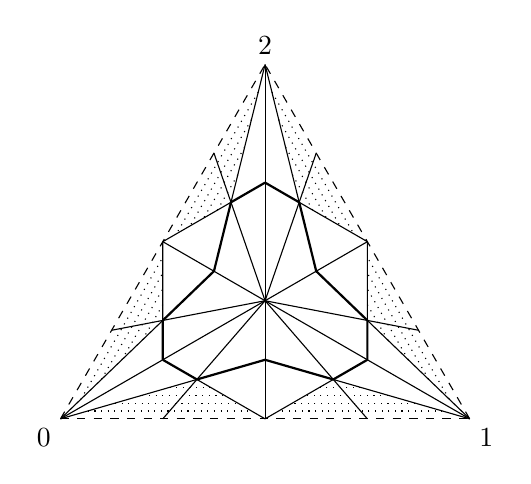
\begin{tikzpicture}

% Vertices of a triangle
\coordinate (2) at (90:3cm);
\coordinate (0) at (210:3cm);
\coordinate (1) at (-30:3cm);

% Nodes to mark vertices of a triangle
\node [above] at (2) {2};
\node [below left] at (0) {0};
\node [below right] at (1) {1};

% Draw line between the vertices 0,1 and 2 and name the midpoints
\draw [dashed] (0.north east)--(2.south) coordinate[midway](02);
\draw [dashed] (0.north east)--(1.north west) coordinate[midway](01);
\draw [dashed] (1.north west)--(2.south) coordinate[midway](12);

% Barycenter, could also be found by means of the intersection library of tikz
\coordinate (012) at (barycentric cs:0=1,1=1,2=1);

% Draws lines from vertices of original triangle to barycentre of original triangle and...
\draw (0.north east)--(012) coordinate[midway](0<012);
\draw (1.north west)--(012) coordinate[midway](1<012);
\draw (2.south)--(012) coordinate[midway](2<012);
\draw (01)--(012) coordinate[midway](01<012);
\draw (12)--(012) coordinate[midway](12<012);
\draw (02)--(012) coordinate[midway](02<012);

% Subdivide each of the six new 2-simplices. To highlight the structure of the desingularized simplicial set we make certain lines thicker
\coordinate (0<01<012) at (barycentric cs:0=1,01=1,012=1);
\coordinate (0<01) at (barycentric cs:0=0.5,01=0.5);
\foreach \x in {(0),(0<01),(01),(012)}
	\draw (0<01<012)--\x;
\foreach \x in {(0<012),(01<012)}
	\draw [thick] (0<01<012)--\x;

\coordinate (1<01<012) at (barycentric cs:1=1,01=1,012=1);
\coordinate (1<01) at (barycentric cs:1=0.5,01=0.5);
\foreach \x in {(1),(1<01),(01),(012)}
	\draw (1<01<012)--\x;
\foreach \x in {(01<012),(1<012)}
	\draw [thick] (1<01<012)--\x;

\coordinate (1<12<012) at (barycentric cs:1=1,12=1,012=1);
\coordinate (1<12) at (barycentric cs:1=0.5,12=0.5);
\foreach \x in {(1),(1<12),(12),(012)}
	\draw (1<12<012)--\x;
\foreach \x in {(12<012),(1<012)}
	\draw [thick] (1<12<012)--\x;

\coordinate (2<12<012) at (barycentric cs:2=1,12=1,012=1);
\coordinate (2<12) at (barycentric cs:2=0.5,12=0.5);
\foreach \x in {(2),(2<12),(12),(012)}
	\draw (2<12<012)--\x;
\foreach \x in {(12<012),(2<012)}
	\draw [thick] (2<12<012)--\x;
	
\coordinate (2<02<012) at (barycentric cs:2=1,02=1,012=1);
\coordinate (2<02) at (barycentric cs:2=0.5,02=0.5);
\foreach \x in {(2),(2<02),(02),(012)}
	\draw (2<02<012)--\x;
\foreach \x in {(02<012),(2<012)}
	\draw [thick] (2<02<012)--\x;
	
\coordinate (0<02<012) at (barycentric cs:0=1,02=1,012=1);
\coordinate (0<02) at (barycentric cs:0=0.5,02=0.5);
\foreach \x in {(0),(0<02),(02),(012)}
	\draw (0<02<012)--\x;
\foreach \x in {(02<012),(0<012)}
	\draw [thick] (0<02<012)--\x;

% Effect of desingularizing doubly subdivided 2-simplex with collapsed boundary. We make these lines dotted.
\foreach \x in {0.2,0.4,0.6,0.8}
	\draw [dotted] (barycentric cs:0=\x,0<01<012=1-\x)--(barycentric cs:01=\x,0<01<012=1-\x);

\foreach \x in {0.2,0.4,0.6,0.8}
	\draw [dotted] (barycentric cs:1=\x,1<01<012=1-\x)--(barycentric cs:01=\x,1<01<012=1-\x);

\foreach \x in {0.2,0.4,0.6,0.8}
	\draw [dotted] (barycentric cs:1=\x,1<12<012=1-\x)--(barycentric cs:12=\x,1<12<012=1-\x);

\foreach \x in {0.2,0.4,0.6,0.8}
	\draw [dotted] (barycentric cs:2=\x,2<12<012=1-\x)--(barycentric cs:12=\x,2<12<012=1-\x);

\foreach \x in {0.2,0.4,0.6,0.8}
	\draw [dotted] (barycentric cs:2=\x,2<02<012=1-\x)--(barycentric cs:02=\x,2<02<012=1-\x);

\foreach \x in {0.2,0.4,0.6,0.8}
	\draw [dotted] (barycentric cs:0=\x,0<02<012=1-\x)--(barycentric cs:02=\x,0<02<012=1-\x);
\end{tikzpicture}
\caption{Desingularizing the double subdivision of the standard $2$-simplex with collapsed boundary.}
\label{fig:ch1_Desing_doublysubd_2simpl}
\end{figure}


By Ken Brown's lemma \cite[Lem.~1.1.12, p.~6]{Ho99} a left Quillen functor takes each weak equivalence between cofibrant objects to a weak equivalence. However, $DSd(d_{\Delta [2]/\partial \Delta [2]})$ is not a weak equivalence. Thus $DSd$ is not a left Quillen functor.
\end{proof}
\noindent Moreover, the diagram
\begin{displaymath}
\xymatrix{
DSd^2(\Delta [2]) \ar[d]^\sim & DSd^2(\partial \Delta [2]) \ar[l] \ar[d]^\sim \ar[r] & DSd^2(\Delta [0]) \ar[d]^\sim \\
DSd(\Delta [2]) & DSd(\partial \Delta [2]) \ar[l] \ar[r] & DSd(\Delta [0])
}
\end{displaymath}
indicates that the map $DSd(\partial \Delta [2])\to DSd(\Delta [2])$ is most likely a non-candidate for a cofibration whenever $nsSet$ is a left proper model category. \cref{lem:non-candidate_cofibration} below justifies this educated guess.

We recall the axiom of propriety, which is desirable in a model category. Consider a commutative square
\begin{displaymath}
 \xymatrix{
 X \ar[d]_i \ar[r]^f & Z \ar[d]^j \\
 Y \ar[r]_g & W
 }
\end{displaymath}
in some category. If the square is cartesian, then we say that $f$ is the \textbf{base change of $g$ along $j$}. If it is cocartesian, then we say that $g$ is the \textbf{cobase change of $f$ along $i$}.
\begin{definition}
Consider a model category. We say that the model category is \textbf{right proper} if weak equivalences are preserved under taking base change along fibrations. Consider a model category. We say that the model category is \textbf{left proper} if weak equivalences are preserved under taking cobase change along cofibrations. If a model category is both right proper and left proper, then we say that it is \textbf{proper}.
\end{definition}
\noindent Note that $sSet$ with the standard model structure is proper \cite[Thm.~13.1.13, p.~242]{Hi03}.

There is a glueing lemma that says that if we have a commutative diagram
\begin{displaymath}
\xymatrix{
B \ar[d]^\sim & A \ar[l] \ar[d]^\sim \ar[r] & C \ar[d]^\sim \\
Y & X \ar[l] \ar[r] & Z
}
\end{displaymath}
in a left proper model category such that at least one map in each row is a cofibration and such that all the vertical maps are weak equivalences, then the canonical map
\[B\sqcup _AC\xrightarrow{\sim } Y\sqcup _XZ\]
of pushouts is a weak equivalence. A reference for the dual of this result is Proposition 13.3.9 in Hirschhorn's book \cite[pp.~246--247]{Hi03}. Note that a more common glueing lemma demands that $A\to B$ and $X\to Y$ be cofibrations and not simply that at least one map in each row be a cofibration.

The former of the two versions of the glueing lemma yields the following result.
\begin{lemma}\label{lem:non-candidate_cofibration}
Assume that $nsSet$ is given a model structure such that it is a left proper model category whose weak equivalences are those maps $f$ such that $\lvert Uf\rvert$ is a (weak) homotopy equivalence. Then neither of the two maps
\[DSd(\partial \Delta [2])\to DSd(\Delta [2])\]
and
\[DSd(\partial \Delta [2])\to DSd(\Delta [0])\]
is a cofibration or neither of the two maps
\[DSd^2(\partial \Delta [2])\to DSd^2(\Delta [2])\]
and
\[DSd^2(\partial \Delta [2])\to DSd^2(\Delta [0])\]
is a cofibration.
\end{lemma}
\noindent \cref{lem:non-candidate_cofibration} justifies the educated guess that $DSd(\partial \Delta [2])\to DSd(\Delta [2])$ is most likely not a cofibration, though it does not imply that the map is not a cofibration.

Before we can state the nature of these properties we need a few definitions. Let $\varepsilon ^n_j:[0]\to [n]$ be the \textbf{vertex operator} given by $0\mapsto j$. Usually, we omit the upper index.
\begin{definition}
Let $X$ be a simplicial set, and $A$ a simplicial subset. We say that $A$ is \textbf{full} if it has the property that any simplex of $X$ is a simplex of $A$ provided its vertices
are in $A$.
\end{definition}
\begin{definition}
Suppose $X$ a simplicial set. Let $A$ be a full simplicial subset of $X$. We say that $A$ is an \textbf{eden (resp. abyss)} in $X$ if it has the property that any $1$-simplex $x$ of $X$ whose first (resp. zeroth) vertex $x\varepsilon _1$ (resp. $x\varepsilon _0$) is in $A$, is itself is a simplex of $A$.
\end{definition}
\noindent We wish to compare the new notions with analogous notions in the $Cat$, partly because the intuition is more readily available in $Cat$ than in $sSet$.

Consider the notions of sieve and cosieve.
\begin{definition}
Suppose $\mathscr{C}$ a small category. Let $\mathscr{D}$ be a subcategory of $\mathscr{C}$. We will say that $\mathscr{D}$ is a \textbf{(co)sieve} in $\mathscr{C}$ if whenever we have a morphism $c\to c'$ whose target (source) is an object of $\mathscr{D}$, then the morphism is itself a morphism of $\mathscr{D}$.
\end{definition}
\noindent Intuitively, a sieve is a place to which there is no entry and a cosieve is a place from which there is no escape. The notion of sieve corresponds to the notion of eden and the notion of cosieve corresponds to the notion of abyss. In $PoSet$, the notion of sieve is equivalent to the notion of ideal when a poset is thought of as a set equipped with a reflexive, antisymmetric and transitive binary operation.

Note the following relationship between the notions of sieve and eden and between cosieve and abyss.
\begin{lemma}\label{lem:nerve_of_(co)sieve}
The nerve of a sieve (resp. cosieve) is an eden (resp. abyss).
\end{lemma}
\noindent Furthermore, note the following characterization.
\begin{lemma}\label{lem:(co)sieve_characterization_elementary}
A simplicial subset $A$ of a simplicial set $X$ is an eden in $X$ if and only if any simplex whose last vertex is in $A$ is also a simplex of $A$. Similarly, the simplicial subset $A$ is an abyss in $X$ if and only if any simplex whose zeroth vertex is in $A$ is also a simplex of $A$.
\end{lemma}
\noindent \cref{lem:(co)sieve_characterization_categorical} below provides another characterization that is more useful.

Performing desingularization is messy in general. However, there are useful situations in which the process is predictable. Such as when one desingularizes a quotient $X/A$ of a non-singular simplicial set $X$ by an eden $A$. \cref{prop:desingularizing_after_collapsing_elysium} will make this precise. Understanding the behavior of $D$ towards quotients of the kind we mentioned is vital to our discussion of the properties of Str\o m maps.

The new notions are of the following categorical nature.
\begin{lemma}\label{lem:(co)sieve_characterization_categorical}
A simplicial subset $A$ of a simplicial set $X$ is an eden (resp. abyss) if and only if there is a map
$\chi :X\rightarrow \Delta [1]$ such that the square
\begin{displaymath}
 \xymatrix{
 A \ar[d] \ar[r] & \Delta [0] \ar[d]^{N\varepsilon _0\; (\textrm{resp.} \; N\varepsilon _1)} \\
 X \ar[r]_(.45)\chi & \Delta [1]
 }
\end{displaymath}
is cartesian. Here,
\[\varepsilon _0:[0]\to [1]\; (\textrm{resp.} \; \varepsilon _1:[0]\to [1])\]
is the vertex operator given by
\[0\mapsto 0\; (\textrm{resp.} \; 0\mapsto 1).\]
We refer to $\chi$ as the \textbf{characteristic map of $A$ as an eden (resp. abyss) in $B$}.
\end{lemma}
\noindent The proof of this lemma is straight-forward, and is left out.

Part of the interest in the notion of eden is that the Kan subdivision creates edens from arbitrary simplicial subsets, which we state as \cref{lemma_subdivision_creates_left_sieve} below. First, we remind the reader how to define the Kan subdivision.

Consider a simplicial set $X$ and the poset $X^\sharp$ of non-degenerate simplices. There is a morphism $y\to x$ from $y$ to $x$ if $y$ is a face of $x$. The operation of taking a simplicial set $X$ to $X^\sharp$ defines a functor $(-)^\sharp :sSet\to PoSet$.  A map $f:X\to Y$ induces the map $f^\sharp :X^\sharp \to Y^\sharp$ given by sending $x$ to the non-degenerate part $f(x)^\sharp$ of $f(x)$.
\begin{lemma}\label{lem:sharp_creates_sieves}
Let $X$ be a simplicial set and let $A$ be a simplicial subset of $X$. Then $A^\sharp$ is a sieve in $X^\sharp$.
\end{lemma}
\noindent This observation will be used in the proof of \cref{lem:Barratt_nerve_of_inclusion_of_non-sing_is_strom} below.
\begin{definition}\label{def:Barratt_nerve}
We refer to the endofunctor of simplicial sets defined on objects by $BX=N(X^\sharp )$ as the \textbf{Barratt nerve}.
\end{definition}
\noindent Note that this terminology is not standard. We follow \cite[Def.~2.2.3, p.~35]{WJR13}, but Fritsch and Piccinini call $B$ the \emph{star functor} \cite[Exercise~4.6.33,~p.~219]{FP90}. The \textbf{Kan subdivision} is the left Kan extension of $B$ along the Yoneda embedding $\Upsilon :\Delta \to sSet$. Loosely, the Kan subdivision is the best way to adapt \emph{barycentric subdivision} to simplicial sets.

We can elaborate the previous paragraph. The \textbf{simplex category} of $X$, denoted $\Delta \downarrow X$, is the small category whose objects are the representing maps $\bar{x}$ of simplices of $X$ and whose morphisms $\bar{y} \to \bar{x}$ are the commutative diagrams
\begin{displaymath}
\xymatrix@=1em{
\Delta [m] \ar[dr]_{\bar{y} } \ar[rr]^{\alpha } && \Delta [n] \ar[ld]^{\bar{x} } \\
& X
}
\end{displaymath}
whenever $y$ is of degree $m$ and $x$ is of degree $n$. Note that we simplify the notation slightly by writing $\alpha$ in place of $N\alpha$, where $\alpha :[m]\to [n]$ must by definition be an operator such that $y=x\alpha$.

One can view the Kan subdivision of $X$ as
\[Sd\; X\cong colim(B\circ \Upsilon _X),\]
where $\Upsilon _X:\Delta \downarrow X\to sSet$ is the composite of Yoneda embedding $[n]\xmapsto{\Upsilon } \Delta [n]$ with the forgetful functor $(x,n)\mapsto [n]$. A simplicial map $f:X\to Y$ gives rise to a functor $\Delta \downarrow f$ such that $\Upsilon _X=\Upsilon _Y\circ \Delta \downarrow f$. In particular, the identity is a natural transformation
\[\Upsilon _X\Rightarrow\Upsilon _Y\circ \Delta \downarrow f.\]
From this arises the map $Sd(f):Sd\, X\to Sd\, Y$ in an intuitive way.

Combining the diagram $B\circ \Upsilon _Y$ with its colimit $Sd\, Y$ gives rise to a cocone on $B\circ \Upsilon _Y\circ \Delta \downarrow f$ with apex $Sd\, Y$ and thus a map
\[colim(B\circ \Upsilon _Y\circ \Delta \downarrow f)\to Sd\, Y.\]
The identity natural transformation $\Upsilon _X\Rightarrow\Upsilon _Y\circ \Delta \downarrow f$ gives rise to a natural transformation
\[B\circ \Upsilon _X\Rightarrow B\circ \Upsilon _Y\circ \Delta \downarrow f,\]
which must be the identity as well. Thus the map above with target $Sd\, Y$ can be considered to have $Sd\, X$ as its source. The map itself is denoted $Sd(f)$.

We can take the viewpoint that
\[X\cong colim(\Upsilon X)\]
\cite[Lem.~4.2.1~(ii),~p.~141]{FP90}. In other words, the cocone $\Upsilon _X\Rightarrow \underline{X}$, meaning the natural transformation from $\Upsilon _X$ to the constant diagram that takes every object to $X$, is universal. Combining this with $B$ yields a cocone $B\circ \Upsilon _X\Rightarrow \underline{BX}$ with apex $BX$. It gives rise to a canonical map $b_X:Sd\, X\to BX$.
\begin{lemma}
\label{lem:properties_of_b_X}
The canonical map $b_X:Sd\, X\to BX$ is natural, degreewise surjective and an isomorphism if and only if $X$ is non-singular.
\end{lemma}
\begin{proof}
The naturality is automatic when $b_X$ comes from the viewpoint that $Sd$ is the left Kan extension of $B$ along the Yoneda embedding. See \cite[Lem.~2.2.10, p.~38]{WJR13} for the statement and proof that $b_X$ is degreewise surjective. See \cite[Lem.~2.2.11, p.~38]{WJR13} for the statement and proof that $b_X$ is an isomorphism if and only if $X$ is non-singular.
\end{proof}
\noindent We will make use of the comparison map $b_X$ in the proof of the crucial result stated as \cref{cor:two-fold_subdivision_strom}.

As promised, the Kan subdivision creates sieves.
\begin{lemma}\label{lemma_subdivision_creates_left_sieve}
Let $X$ be a simplicial set and $A$ a simplicial subset. Then $\textrm{Sd} \, A$ is an eden in $\textrm{Sd} \, X$.
\end{lemma}
\begin{proof}[Proof of Lemma~\ref{lemma_subdivision_creates_left_sieve}]
Let $i:A\to X$ be the inclusion. We will construct a natural transformation
\[B\circ \Upsilon _X\xRightarrow{\psi } \underline{\Delta [1]},\]
which gives rise to a map $\chi :\textrm{Sd} \,X\to \Delta [1]$. Next, we will verify that $Sd\, A\to \Delta [0]$ is a base change of $\chi$ along $N\varepsilon _0$.

Given an object $\bar{x} :\Delta [n]\to X$ of $\Delta \downarrow X$ we define
\[\psi _{\bar{x} }:B(\Delta [n])\to \Delta [1]\]
by letting it be the nerve of $\Delta [n]^\sharp \to [1]$ given by sending an object $\mu$ of $\Delta [n]^\sharp$ to $0$ if $x\mu$ is a simplex of $A$, and to $1$ otherwise.

We verify that the triangle
\begin{displaymath}
\xymatrix@=1em{
 B(\Delta [m]) \ar[dd]_{B(N\alpha )} \ar[dr]^{\psi _{\bar{y} }} \\
 & \Delta [1] \\
 B(\Delta [n]) \ar[ur]_{\psi _{\bar{x} }}
 }
\end{displaymath}
commutes whenever $\alpha$ is such that $y=x\alpha$. To this end, take some face operator $\mu \in \Delta [m]^\sharp$ with target $[m]$. The order-preserving function $(N\alpha )^\sharp$ sends $\mu$ to the face operator $(\alpha \mu )^\sharp$. We can write $y\mu$ as a degeneracy
\[y\mu =x\alpha \mu =x(\alpha \mu )^\sharp (\alpha \mu )^\flat\]
of $x(\alpha \mu )^\sharp$. This means that $y\mu$ is a simplex of $A$ if and only if $x(\alpha \mu )^\sharp$ is a simplex of $A$. In other words, the underlying triangle of posets commutes. Thus $\psi _{\bar{x} }$ is natural, as claimed.

As a result of the previous paragraph we now have the composite natural transformation
\[B\circ \Upsilon _X\Rightarrow \underline{Sd\, X} \Rightarrow \underline{\Delta [1]} \]
between functors $\Delta \downarrow X\to sSet$. This composite induces a composite of natural transformations between functors $\Delta \downarrow A\to sSet$, through precomposition with $\Delta \downarrow i$. By the design of $\psi$, the latter factors through $N\varepsilon _0:\Delta [0]\to \Delta [1]$. This way we obtain a commutative square
\begin{displaymath}
\xymatrix{
B\circ \Upsilon X\circ \Delta \downarrow i \ar@{=>}[d] \ar@{==>}[r] & \underline{\Delta [0]} \ar@{=>}[d]^{\underline{N\varepsilon _0} } \\
\underline{Sd\, X} \ar@{=>}[r] & \underline{\Delta [1]}
}
\end{displaymath}
of natural transformations and thus a candidate $\chi :Sd\, X\to \Delta [1]$ for a characteristic map. It remains to verify that, if given a solid arrow commutative diagram
\begin{displaymath}
 \xymatrix{
 Z \ar@/^2pc/[drr] \ar@{-->}[dr] \ar@/_2pc/[ddr]_f \\
 & Sd\, A \ar[d]_{Sd(i)} \ar[r] & \Delta [0] \ar[d]^{N\varepsilon _0} \\
 & Sd\, X \ar[r]_(.45)\chi & \Delta [1]
 }
\end{displaymath}
then there exists a dashed map $Z\to Sd\, A$ that makes the whole diagram commute. There is at most one such map $Z\to Sd\, A$ as $Sd(i)$ is degreewise injective. Because $\Delta [0]$ is a terminal object it is enough to verify that $f$ factors through $Sd(i)$. As $Sd(i)$ is degreewise injective it suffices to verify that the image of $f$ is contained in the image of $Sd(i)$.

Suppose $z$ a $q$-simplex of $Z$. By the commutativity of the solid arrow diagram, we get that
\[N\varepsilon _0 \circ g(z)=\chi \circ f(z).\]
We argue that $f(z)\in Sd(X)_q$ is in the image of $Sd(i)_q$.

The simplex $f(z)$ is the image of some element $\varphi :[q]\to \Delta [n]^\sharp \in \Upsilon _X(\bar{x} )$ such that $\varphi (q)$ is the identity. Write $\varphi _j=\varphi (j)$ for $0\leq j\leq q$. Because $\chi \circ f(z)$ is in the image of $N\varepsilon _0$, it follows that $x\varphi _j$ is a simplex of $A$ for each $j$ with $0\leq j\leq q$. In particular, the simplex $x\varphi _q$ is a simplex of $A$. The face operator $\varphi _q$ is the identity, so $x=x\varphi _q$ is itself a simplex of $A$. Thus $f(z)$ is in the image of $Sd(i)$.
\end{proof}
\noindent Now we know that a simplicial subset of a simplicial set can always be turned into an eden by applying the Kan subdivision.

The following term is central.
\begin{definition}\label{def:strom}
A map $k:A\to B$ in $nsSet$ is referred to as a \textbf{Strøm map} if the following conditions hold.
\begin{enumerate}
\item{The map $k$ is a degreewise injective map whose image is an eden in $B$.}
\item{There is an abyss $W$ in $B$ such that $k$ can be factored as $i:A\to W$ followed by the inclusion $j:W\to B$.}
\item{The map $i$ is a section of some map $r:W\to A$.}
\item{The simplicial set $W$ is deformable rel $A$ to $A$ in $W$, namely there exists a simplicial homotopy $\epsilon :W\times \Delta [1]\to W$ such that the diagrams
\begin{displaymath}
\xymatrix{
W \ar[d]_{i_0} \ar[dr]^{ir} && A\times \Delta [1] \ar[dd]_{pr_1} \ar[r]^{i\times1} & W\times \Delta [1] \ar[dd]_{\epsilon } \\
W\times \Delta [1] \ar[r]^\epsilon & W  \\
W \ar[u]^{i_1} \ar[ur]_1 && A \ar[r]^i & W
}
\end{displaymath}
commute.}
\end{enumerate}
\end{definition}
\noindent Notice that the image of $k$ is an eden in $W$.

The class of Str\o m maps is not a category as a composite of Str\o m maps is not necessarily a Str\o m map. This is because the two simplicial homotopies as described in \cref{def:strom} that come with two composable Str\o m maps do not necessarily give rise to a new simplicial homotopy that satisfies the fourth condition of \cref{def:strom}. Compare with class of pseudo-Dwyer maps \cite{Ci99}, which does form a subcategory of $Cat$.

A bit of history may be of interest to the reader. The class of Str\o m maps fills the same role in establishing $nsSet$ as a model category (Quillen equivalent to $sSet$) as the class of \emph{Dwyer maps} in Thomason's paper \cite{Th80}, where $Cat$ is established as a model category (Quillen equivalent to $sSet$). However, a mistake in Thomason's proof intially left the axiom of propriety unproven.

After having established the model structure, Thomason asserted that the Dwyer maps were closed under retracts. As any cofibration was a retract of a Dwyer map, Thomason concluded that any cofibration was a Dwyer map. Therefore, as the nerve functor $N$ took a cocartesian square in $Cat$ with at least one leg Dwyer to a homotopy cocartesian square in $sSet$, it would follow that $Cat$ is left proper. However, the Dwyer maps are not closed under retracts \cite{Ci99}.

This mistake was not a fatal mistake, as it turned out. Cisinski was able to correct the proof of the axiom of propriety by weakening the definition of the term Dwyer map and thus creating a new notion that he gave the ad hoc name \emph{pseudo-Dwyer map}. Perhaps the new notion is better referred to under the name \emph{Cisinski map}. The notion of Cisinski map may have been borrowed from A. Str\o m as it is an analogue to one of his characterizations \cite[Thm.~2~(ii), p.~12]{St66} of the cofibrations for the Str\o m model structure on topological spaces \cite{St72}. It is the model structure whose weak equivalences are the homotopy equivalences and whose fibrations are the Hurewicz fibrations.

Cisinski argues that $N$ takes a cocartesian square in $Cat$ with at least one leg Cisinski to a homotopy cocartesian square in $sSet$ \cite{Ci99}. Thus Thomason's argument that $Cat$ is left proper goes through when Dwyer maps are replaced by Cisinski maps. Cisinski takes the correction one step further and points out that Cisinski maps are closed under cobase change and under taking compositions of $\aleph _0$-sequences \cite{Ci99}. Indeed, Raptis points out that both Dwyer maps and Cisinski maps are closed under (transfinite) compositions \cite[Prop.~2.4.~(a),~p.~216]{Ra10}. Thus, using Thomason's original technique, Thomason's model structure on $Cat$ can be established by means of the term Cisinski map alone, although the notion of Dwyer map plays a role in Thomason's discussion regarding cofibrant objects \cite[Lemma 5.6.~(4),p.~323]{Th80}.

Crucially, the sets $DSd^2(I)$ and $DSd^2(J)$ are contained in the class of Str\o m maps, as we will now argue.
\begin{lemma}\label{lem:Barratt_nerve_of_inclusion_of_non-sing_is_strom}
Let $k:A\to X$ be an inclusion of a simplicial subset $A$ into a non-singular simplicial set $X$. If $A$ is an eden in $X$, then $B(k)$ is a Str\o m map.
\end{lemma}
\begin{proof}
Let $W$ be the subposet of $X^\sharp$ whose objects are precisely the non-degenerate simplices of $X$ that have a face in $A$. As $A$ is an eden it follows that there is a greatest face in $A$ of any given element of $W$. If $w\in W$, we let $r(w)$ denote this unique face. Because $X$ is non-singular it follows that $r(w)$ is non-degenerate, hence an object of $A^\sharp$. Moreover, we get a functor $r:W\to A^\sharp$. It is a retraction of the corestriction $i$ of $k^\sharp :A^\sharp \to X^\sharp$ to $W$.

By \cref{lem:sharp_creates_sieves}, the functor $(-)^\sharp$ creates sieves. Therefore, we get that $A^\sharp$ is a sieve in $X^\sharp$. By the definition of $W$ it follows that it is a cosieve in $X^\sharp$. Furthermore, \cref{lem:nerve_of_(co)sieve} says that $BA=N(A^\sharp )$ is an eden in $BX=N(X^\sharp )$ and that $NW$ is an abyss in $BX$.

If $w\in W$, then there is a morphism $ir(w)\to w$ by the definition of $r$. The rest of the argument is standard. Namely, because $W$ is a poset it is true that $ir(w)\to w$ is automatically natural. This natural morphism from $ir$ to the identity can be viewed as a functor $W\times [1]\to W$, which in turn gives rise to a simplicial homotopy $NW\times \Delta [1]\to NW$ from $Ni\circ Nr$ to the identity as $N$ preserves limits and in particular products. The simplicial homotopy is stationary on $N(A^\sharp )$ because it is identified with the nerve of $W\times [1]\to W$, which is stationary on $A^\sharp$ in an intuitive, analogous sense. This concludes the proof that $B(k)$ is a Str\o m map.
\end{proof}
\begin{corollary}\label{cor:two-fold_subdivision_strom}
Let $Y$ be a simplicial set such that $Sd\, Y$ is non-singular and let $X$ be a simplicial subset of $Y$. If $k:X\to Y$ is the inclusion, then $Sd^2(k)$ is Str\o m.
\end{corollary}
\begin{proof}
According to \cref{lemma_subdivision_creates_left_sieve}, we have that $Sd\, X$ is an eden in $Sd\, Y$. By \cref{lem:Barratt_nerve_of_inclusion_of_non-sing_is_strom} we now know that $BSd(k)$ is Str\o m. The naturality of $b_{Sd\, X}$ means that we can identify $BSd(k)$ with $Sd^2(k)$ via the diagram
\begin{displaymath}
\xymatrix{
Sd^2\, X \ar[d]_{Sd(Sd(k))} \ar[r]^{b_{Sd\, X}}_\cong & BSd\, X \ar[d]^{B(Sd(k))} \\
Sd^2\, Y \ar[r]_{b_{Sd\, Y}}^\cong & BSd\, Y
}
\end{displaymath}
as $Sd\, X$ and $Sd\, Y$ are non-singular. This is because the natural map from the Kan subdivision to the Barratt nerve is an isomorphism when the original simplicial set is non-singular \cite[Lem.~2.2.11, p.~38]{WJR13}. Hence, the map $Sd^2(k)$ is a Str\o m map.
\end{proof}
\noindent In particular, if $k$ in \cref{cor:two-fold_subdivision_strom} is one of the inclusions $\partial \Delta [n]\to \Delta [n]$ or one of the inclusions $\Lambda ^j[n]\to \Delta [n]$, then we see that $Sd^2(k)$ is a Str\o m map.





\section{On higher and lower planes of existence}
\label{sec:planes}

\noindent \cref{cor:two-fold_subdivision_strom} has shown us that the sets $DSd^2(I)$ and $DSd^2(J)$ are both contained in the class of Str\o m maps. This class of maps will serve as an auxiliary class of maps that aids us in establishing the model structure.

To form a pushout in $nsSet$ one can first form the pushout in $sSet$ and then desingularize it. The desingularization process destroys the homotopy type in general, but it turns out that the homotopy type is preserved when the pushout in $sSet$ is taken along a Str\o m map. This result is stated as \cref{lem:Pushout_along_strom_homotopically_wellbehaved}. The important formal property of Str\o m maps is that they are preserved under taking cobase change, which is stated as \cref{prop:Strom-maps_closed_under_cobasechange}. To prove both of these results, the most work intensive task is to establish \cref{prop:desingularizing_after_collapsing_elysium}, which we will focus on in this section. It helps us control the homotopical behavior of desingularization in important cases.

As a preliminary step towards proving that Str\o m maps are preserved under cobase change, we have the following basic result.
\begin{lemma}\label{lem:elysiums_abysses_preserved_cobase_change}
If the square
\begin{displaymath}
\xymatrix{
A \ar[d]_i \ar[r]^f & C \ar[d]^j \\
X \ar[r]_(.35)g & X\sqcup _AC
}
\end{displaymath}
is cocartesian in $sSet$ and $i$ embeds $A$ as an eden (resp. abyss) in $X$ then $j$ embeds $C$ as an eden (resp. abyss) in $X\sqcup _AC$.
\end{lemma}
\begin{proof}
We do the case when $A$ is an eden. Notice that no part of the proof prefers the case when $A$ is an eden over the case when $A$ is an abyss. Alternatively, use the notion of the opposite \cite[Def.~2.2.19, p.~ 42]{WJR13} of a simplial set to conclude that the result also holds in the case when $A$ is an abyss.

Note that we can factor $f:A\to C$ as a degreewise surjective map followed by a degreewise injective map, so we can prove the lemma by proving that it holds in the two cases when $f$ is degreewise surjective or degreewise injective.

First, we do the case when $f$ is degreewise surjective. Suppose $y$ some simplex of $X\sqcup _AC$ whose last vertex is in the image of $j$. We will prove that $y$ is in the image of $g$. Here, we use the elementary characterization from \cref{lem:(co)sieve_characterization_elementary}.

There is at most one simplex $x$ such that $y=g(x)$. Suppose there is one. As $f$ is surjective in degree $0$, there is a $0$-simplex $v$ of $A$ such that
\[y\varepsilon _n=j\circ f(v)=g\circ i(v)\]
by the assumption that $y\varepsilon _n$ is in the image of $j$. As $i$ embeds $A$ as an eden in $X$, there is a simplex $a$ of $A$ such that $x=i(a)$. Then we can define $c=f(a)$. The given simplex $y$ is the image under $j$ of $c$. It follows that $j$ embeds $C$ as an eden in $X\sqcup _AC$.

Finally, we do the case when $f$ is degreewise injective. Suppose $y$ some simplex of $X\sqcup _AC$ whose last vertex is in the image of $j$. We will prove that $y$ is in the image of $g$.

There is at most one simplex $x$ such that $y=g(x)$. Suppose there is one. The vertex $y\varepsilon _n$ is then uniquely the image under $g$ of $x\varepsilon _n$, in addition to being uniquely the image under $j$ of some $0$-simplex $w$ of $C$. Hence, there is some unique $0$-simplex $v$ of $A$ whose images under $f$ and $i$ are $w$ and $x\varepsilon _n$, respectively. Hence, there is some simplex $a$ of $A$ with $x=i(a)$ by the assumption that $i$ embeds $A$ as an eden in $X$. Thus $y$ is the image under $j$ of $c=f(a)$. It follows that $j$ embeds $C$ as an eden in $X\sqcup _AC$.
\end{proof}
\noindent In addition to \cref{lem:elysiums_abysses_preserved_cobase_change}, we will state some basic properties of cartesian squares.

The properties stated in \cref{Lemma_Pullbacks_close_to_twooutofthree_property} below are here collectively referred to as the two-out-of-three property for cartesian squares. See for example III.4 Exercise 8 (b) in \cite{ML98} for a reference to the first two statements of \cref{Lemma_Pullbacks_close_to_twooutofthree_property} below. All three statements of \cref{Lemma_Pullbacks_close_to_twooutofthree_property} appear in Lemma 2.4 of \cite[p.~57]{CPS06} for the case $\mathscr{C} =sSet$ as Chachólski, Pitsch and Scherer work in that category.
\begin{lemma}[Two-out-of-three property for cartesian squares]
\label{Lemma_Pullbacks_close_to_twooutofthree_property}
Suppose
\begin{displaymath}
\xymatrix{
A \ar[d] \ar[r] & C \ar[d] \ar[r] & E \ar[d] \\
B \ar[r] & D \ar[r] & F
}
\end{displaymath}
a diagram in some category $\mathscr{C}$.
\begin{enumerate}
\item{The outer square is cartesian if both the left hand and the right hand square are cartesian squares.}
\item{Likewise, the left hand square is cartesian if the right hand and outer squares are cartesian.}
\item{If the outer and left hand squares are cartesian, then the right hand square is cartesian if the morphism $B\to D$ has a section.}
\end{enumerate}
\end{lemma}
\begin{proof}
Consider the third statement, meaning the case when the left hand and outer squares are cartesian and $k$ has a section, consider the diagram
\begin{displaymath}
\xymatrix{
& X \ar@{-}@/_0.2pc/[d] \ar@{-->}[dr]^\gamma \ar@/^1pc/[drrr]^\epsilon \\
A \ar[d]_f \ar[rr]^(.3)i & \ar@/_/[dr]^(.4)\delta & C \ar[d]^g \ar[rr]^j && E \ar[d]^h \\
B \ar[rr]^k && D \ar@/^1pc/[ll]^s \ar[rr]_l && F
}
\end{displaymath}
in $\mathscr{C}$, where we assume that $h\circ \epsilon =l\circ \delta$.

We will prove the existence and uniqueness of a map $\gamma :X\to C$ such that $\epsilon =j\circ \gamma$ and $\delta =g\circ \gamma$.

First we prove existence. Because the outer square is cartesian and because $s$ is a section of $k$, the two maps $\epsilon$ and $s\circ \delta$ give rise to a map $\alpha :X\to A$ such that
\begin{equation}\label{eq:one_proof_of_Lemma_Pullbacks_close_to_twooutofthree_property}
\epsilon =(j\circ i)\circ \alpha
\end{equation}
and
\begin{equation}\label{eq:two_proof_of_Lemma_Pullbacks_close_to_twooutofthree_property}
s\circ \delta =f\circ \alpha .
\end{equation}
Define $\gamma =i\circ \alpha$. Then (\ref{eq:one_proof_of_Lemma_Pullbacks_close_to_twooutofthree_property}) is the first half of what we need to verify. For the second half, observe that $k$ composed with each side of (\ref{eq:two_proof_of_Lemma_Pullbacks_close_to_twooutofthree_property}) yields
\begin{displaymath}
\begin{array}{rcl}
\delta & = & (k\circ s)\circ \delta \\
& = & k\circ (s\circ \delta ) \\
& = & k\circ (f\circ \alpha ) \\
& = & (k\circ f)\circ \alpha  \\
& = & (g\circ i)\circ \alpha  \\
& = & g\circ (i\circ \alpha ) \\
& = & g\circ \gamma ,
\end{array}
\end{displaymath}
which is the second half of the verification of the existence of $\gamma$.

Finally, we prove uniqueness of $\gamma$. Take two maps $X\to C$, denoted $\gamma$ and $\gamma '$, such that the equations
\begin{displaymath}
\begin{array}{rcl}
\delta & = & g\circ \gamma \\
\delta & = & g\circ \gamma ' \\
\epsilon & = & j\circ \gamma \\
\epsilon & = & j\circ \gamma '
\end{array}
\end{displaymath}
hold. Then the two maps $s\circ \delta$ and $\gamma$ give rise to a canonical map $\alpha :X\to A$ as the left hand square is cartesian. Similarly, the two maps $s\circ \delta$ and $\gamma '$ give rise to a canonical map $\alpha ':X\to A$. Next, we can take advantage of the assumption that the outer square is cartesian. This shows that $\alpha =\alpha '$. Then the equations
\[\gamma =i\circ \alpha =i\circ \alpha '=\gamma '\]
yield the desired uniqueness.
\end{proof}
\noindent Note that the assumption that $B\to D$ is an epimorphism is enough for the third statement of \cref{Lemma_Pullbacks_close_to_twooutofthree_property} to hold for for some categories $\mathscr{C}$. This is trivially true when $\mathscr{C} =Set$ is the category of sets and functions, for the epimorphisms are in that case the surjective functions, which are in turn the functions that have a section.
\begin{corollary}\label{cor:sSet_Pullbacks_close_to_twooutofthree_property}
Suppose
\begin{displaymath}
\xymatrix{
A \ar[d] \ar[r] & C \ar[d] \ar[r] & E \ar[d] \\
B \ar[r] & D \ar[r] & F
}
\end{displaymath}
a diagram in the category $sSet$. If the outer and left hand squares are cartesian, then the right hand square is cartesian if $B\to D$ is degreewise surjective.
\end{corollary}
\begin{proof}
The corollary follows from the third statement of \cref{Lemma_Pullbacks_close_to_twooutofthree_property} in the following way. The category $sSet$ is the category of functors $\Delta ^{op} \to Set$ and natural transformations between them. As a $Set$-valued functor category, the category $sSet$ is bicomplete. In a functor category, limits and colimits are formed pointwise. In other words, we can apply \cref{Lemma_Pullbacks_close_to_twooutofthree_property} in the case when $\mathscr{C} =Set$, in a given degree $n$ as $B_n\to D_n$ is surjective by assumption. The right hand square in degree $n$ is thus cartesian. We can conclude that the right hand square of the given diagram is cartesian in $sSet$
\end{proof}
\noindent Note that \cref{cor:sSet_Pullbacks_close_to_twooutofthree_property} shows that the assumption that $B\to D$ is an epimorphism is sufficient in the case when $\mathscr{C} =sSet$ in \cref{Lemma_Pullbacks_close_to_twooutofthree_property} above.

We are interested in triples $(X,A,V)$ where $X$ is a simplicial set, where $A$ is a non-singular eden in $X$ and where $V$ is a non-singular abyss in $X$. We are particularly interested in two cases. The first is when $A$ is contained in $V$ as this is part of the definition of the term Str\o m map. Secondly, we are interested in the case when $A_0\cup V_0=X_0$ and $A_0\cap V_0=\emptyset$. In this section, we will only consider the second case, however the first case plays a role in the next section.

Notice that if $\chi :X\to \Delta [1]$ is the characteristic map of $A$ as an eden in $X$, then $\chi$ is actually also the characteristic map of $V$ as an abyss in $X$. This is because we are concerned with the special case when $A_0\cup V_0=X_0$ and $A_0\cap V_0=\emptyset$. Therefore, given an $n$-simplex $x$ of $X$ we can consider the diagram
\begin{equation}\label{eq:diagram_proof_of_prop_desingularizing_after_collapsing_elysium}
\begin{gathered}
\xymatrix{
\Delta [k] \ar[d] \ar@{-->}[r] \ar@/^1pc/[rr] & A \ar[d] \ar[r] & \Delta [0] \ar[d]^{N\varepsilon _0} \\
\Delta [n] \ar[r]^{\bar{x} } & X \ar[r]^\chi & \Delta [1] \\
\Delta [n-k-1] \ar[u] \ar@/_1pc/[rr] \ar@{-->}[r] & V \ar[u] \ar[r] & \Delta [0] \ar[u]_{N\varepsilon _1}
}
\end{gathered}
\end{equation}
where we have taken the base changes of $\chi \circ \bar{x}$ along $N\varepsilon _0$ and $N\varepsilon _1$, respectively. Here, we allow $-1\leq k\leq n$ and use the convention $\Delta [-1]=\emptyset$. The vertex $x\varepsilon _j$ is a simplex of $A$ if $j\leq k$ and a simplex of $V$ if $j>k$. The diagram above also illustrates the intuition from \cref{sec:behavior}, which says that a simplex can leave an eden or enter an abyss, but that a simplex can neither enter an eden nor leave an abyss.

Now, consider the case when $x$ is non-degenerate. If $k=-1$, then $x$ is a simplex of $V$, which means that it is embedded in $V$ as $V$ is non-singular. Then $x$ is also embedded in $X$, of course. If $k=n$, then $x$ is a simplex of $A$, which means that it is embedded as $A$ is non-singular. Taking the contrapositive, we get that $k\neq -1$ and that $k\neq n$ if $x$ is not embedded. In particular, it follows that $n>0$ if $x$ is not embedded. But if $n=1$, then $x$ is embedded in the case when $k=0$. This is because $A_0$ and $V_0$ are disjoint and because the vertex $x\varepsilon _0$ is a $0$-simplex of $A$ and because $x\varepsilon _1$ is a $0$-simplex of $V$. So in fact,
\begin{equation}\label{eq:conditions_proof_of_prop_desingularizing_after_collapsing_elysium}
-1\neq k\neq n>1
\end{equation}
when $x$ is non-degenerate and non-embedded.

For the statement of \cref{prop:desingularizing_after_collapsing_elysium}, note that we intend to replace the triple $(X,A,V)$ with the triple $(X/A,\Delta [0],V)$ where $X$ is non-singular. In other words, we specialize quite a lot.
\begin{proposition}\label{prop:desingularizing_after_collapsing_elysium}
Let $X$ be non-singular and $A$ an eden in $X$. Furthermore, consider the cocartesian square
\begin{displaymath}
\xymatrix{
  A \ar[d]_i \ar[r]^f & \Delta [0] \ar[d]^{\bar{\imath} } \\
  X \ar[r]_(.4){\bar{f} } & X/A
}
\end{displaymath}
in $sSet$. If $V$ is the full simplicial subset of $X$ whose $0$-simplices are the ones that are not in $A$, then the composite
\[V\xrightarrow{j} X\xrightarrow{\bar{f} } X/A\xrightarrow{\eta } D(X/A),\]
denoted $\tilde{\jmath }$, is an embedding of $V$ as an abyss in $D(X/A)$.
\end{proposition}
\noindent Notice that $V$ is an abyss in $X$ as $A$ is an eden. It is even true that $V$ is an abyss in $X/A$. If the latter statement is not clear at this time, it will be early in the proof. Thus the triple $(X/A,\Delta [0],V)$ is indeed a specialization from the previous paragraphs.

Recall from the fact that $nsSet$ is a reflective subcategory of $sSet$ that one can make the square from \cref{prop:desingularizing_after_collapsing_elysium} cocartesian in $nsSet$ by desingularizing the pushout $X/A$. Let $\tilde{\imath }$ denote the composite of the canonical map $X/A\xrightarrow{\eta } D(X/A)$ with $\bar{\imath }$. Let $\bar{\jmath } =\bar{f} \circ j$.

The triple $(X,\Delta [0],V)$ is a form of world order, where the eden $\Delta [0]$ can be thought of as a higher plane of existence and the abyss $V$ as a lower plane. A simplex of $X/A$ is thought of as living in this world in the manner explained by the diagram (\ref{eq:diagram_proof_of_prop_desingularizing_after_collapsing_elysium}) and the conditions of (\ref{eq:conditions_proof_of_prop_desingularizing_after_collapsing_elysium}).

We will make use of the following terminology.
\begin{definition}\label{def:hty_sequence}
If $\lambda$ is an ordinal, then a \textbf{$\lambda$-sequence} in a cocomplete category $\mathscr{C}$ is a cocontinous functor $X:\lambda \to \mathscr{C}$, written as
\begin{displaymath}
\xymatrix{
X^{[0]} \ar[r] & X^{[1]} \ar[r] & \cdots \ar[r] & X^{[\beta ]} \ar[r] & \cdots \; ,
}
\end{displaymath}
$\beta <\lambda$. The canonical map
\[X^{[0]}\to colim_{\beta <\lambda }X^{[\beta ]}\]
is the \textbf{composition} of the $\lambda$-sequence. A \textbf{sequence} is a $\lambda$-sequence for some ordinal $\lambda$.
\end{definition}
\noindent For sequences, we sometimes use the same letters that at other times denote simplicial sets. However, we use the brackets in the notation to avoid confusion with skeleton filtrations. This is because $X^n$, $n\geq 0$, denotes the $n$-skeleton of a simplicial set $X$. Also recall that we have taken $X_n$, $n\geq 0$, to mean the set of $n$-simplices of a simplicial set $X$. Both of the two latter notations are standard.

Next, we prove the proposition.
\begin{proof}[Proof of \cref{prop:desingularizing_after_collapsing_elysium}]
We will desingularize the simplicial set $X/A$ in an iterative manner. Each non-embedded non-degenerate simplex of $X/A$ will be made degenerate.

The method we use is similar to how G. Lewis Jr. makes a $k$-space compactly generated by identifying two points whenever they cannot be separated by open sets \cite[p.~158]{Le78}.

Our method is also a modification of \cref{thm:main_result_itdesing}. Moreover, the simplicial set $X/A$ is quite special as it is formed by collapsing an eden within a non-singular simplicial set. This makes it viable to deal with one non-embedded non-degenerate simplex at a time. Doing this seems to maximize the transparency of the process so that it becomes easy to realize that $V$ stays an abyss during the process. This is the reason we modify the theory in \cref{sec:calculations} and \cref{sec:description} instead of applying the general result that is \cref{thm:main_result_itdesing}. Recall that $V$ is defined as the full simplicial subset of $X$ whose $0$-simplices are the ones that are not in $A$.

The canonical map $\bar{\imath }$ is by \cref{lem:elysiums_abysses_preserved_cobase_change} an embedding of $\Delta [0]$ as a eden, which says precisely that the first quadrant of the diagram
\begin{displaymath}
 \xymatrix{
  A \ar[d]_i \ar[r] & \Delta [0] \ar[d]^{\bar{\imath } } \ar[r] & \Delta [0] \ar[d]^{N\varepsilon _0} \\
  X \ar@{->>}[r]^(.4){\bar{f} } & X/A \ar@{-->}[r]^{\bar{\chi } } & \Delta [1] \\
  V \ar[u]^j \ar@{-->}[r]_\cong \ar[ur]_{\bar{\jmath } } & V' \ar[u] \ar[r] & \Delta [0] \ar[u]_{N\varepsilon _1}
 }
\end{displaymath}
is cartesian. This yields the canonical map $\bar{\chi }$. In addition, we have formed the cartesian square in the fourth quadrant, which yields the map $V\to V'$. Next, we will argue that the latter map is an isomorphism.

We start by proving that $V\to V'$ is degreewise surjective. The outer part of the lower half is cartesian and so is the fourth quadrant. By \cref{Lemma_Pullbacks_close_to_twooutofthree_property} it then follows that the third quadrant is also cartesian. Hence, the map $V\to V'$ is a base change of the degreewise surjective map $\bar{f}$. Limits in $sSet$ are computed in each degree, and in the category of sets, a base change of a surjective map is again surjective. We can conclude that $V_q\to V_q'$ is surjective
for each $q\geq 0$.

Next, we argue that $V\to V'$ is degreewise injective. Consider the diagram
\begin{displaymath}
\xymatrix{
 V \ar[d]_j & \emptyset \ar[l] \ar[d] \ar[r] & \Delta [0] \ar[d] \\
 X & A \ar[l]^i \ar[r]_(.45)f & \Delta [0]
 }
\end{displaymath}
which gives rise to a canonical map $V\sqcup \Delta [0]\to X/A$ between pushouts in $SSet$. As $A$ is an eden in $X$ and by the definition of $V$, the images of $i$ and $j$ are disjoint. Hence, the map between pushouts is degreewise injective. In particular, the composite $\bar{\jmath }$ is degreewise injective, implying that $V\to V'$ is. In other words, the canonical map $V\xrightarrow{\cong } V'$ is an isomorphism.

We are ready to begin the iterative desingularization of $X/A$. Let $p^0$ be the canonical degreewise surjective map $X/A\xrightarrow{\eta _{X/A} } D(X/A)$ and write
\[D^{[0]}(X/A)=X/A.\]
Here, we use brackets, because we intend to describe a sequence. This is to make the notation reflect that of  \cref{def:hty_sequence}

Furthermore, write
\begin{displaymath}
\begin{array}{rcl}
i^0 & = & \bar{\imath } \\
j^0 & = & \bar{\imath } \\
\chi ^0 & = & \bar{\chi } .
\end{array}
\end{displaymath}
Assume that we for some ordinal $\gamma >0$ have a $\gamma$-sequence of commutative diagrams
\begin{displaymath}
\xymatrix{
& \Delta [0] \ar[ld]_{\tilde{i} } \ar[d]_{i^\beta } \ar[r] & \Delta [0] \ar[d]^{N\varepsilon _0} \\
D(X/A) & D^{[\beta ]}(X/A) \ar[l]_(.45){p^\beta } \ar[r]^(.6){\chi ^\beta } & \Delta [1] \\
& V \ar[lu]^{\tilde{j} } \ar[u]^{j^\beta } \ar[r] & \Delta [0] \ar[u]_{N\varepsilon _1}
}
\end{displaymath}
for $\beta <\gamma$ where\dots
\begin{enumerate}
\item{\dots the two squares are cartesian, where\dots}
\item{\dots $p^\beta$ is degreewise surjective for each $\beta <\gamma$ and where\dots}
\item{\dots each map $D^{[\alpha ]}(X/A)\xrightarrow{f^{\alpha ,\beta }} D^{[\beta ]}(X/A)$, $0\leq \alpha \leq \beta <\gamma$, is also degreewise surjective.}
\end{enumerate}
By the phrase \emph{$\gamma$-sequence of commutative diagrams} used above we mean a functor from the ordinal $\gamma$ to the category of functors whose source is the category
\begin{displaymath}
\xymatrix{
& 2 \ar[ld] \ar[d] \ar[r] & 1 \ar[d] \\
3 & 6 \ar[l] \ar[r] & 0 \\
& 4 \ar[lu] \ar[u] \ar[r] & 5 \ar[u]
}
\end{displaymath}
and whose target is $sSet$. Thus compatibility of all the maps above is implicit in the hypothesis. We will refer to the commutative diagram with index $\beta$ as the \textbf{$\beta$-th stage} of the (iterative) desingularization process, and even to $D^{[\beta ]}(X/A)$ under the same name.

If a simplicial set is not non-singular, then we say that it is \textbf{singular}. Together with the $\gamma$-sequence, assume that for each ordinal $\beta <\gamma$ such that $D^{[\beta ]}(X/A)$ is singular, we have a simplex $x^\beta$ of $X$ such that $f^{0,\beta }(x^\beta )$ is a non-embedded non-degenerate simplex of $D^{[\beta ]}(X/A)$. Suppose $x^\alpha \neq x^\beta$ whenever $\alpha \neq \beta$. Assume that for each ordinal $\beta$ such that $\beta +1<\gamma$, we have that the simplex $f^{0,\beta +1}(x^\beta )$ of $D^{[\beta +1]}(X/A)$ is degenerate. This data will later be used in proving that the iterative desingularizing process does indeed come to a halt.

If $D^{[\gamma ]}(X/A)$ is singular, then let $x^\gamma$ be a simplex of $X/A$ whose image under $f^{0,\gamma }$ is a non-embedded non-degenerate simplex. Suppose $\beta <\gamma$. Notice that $x^\beta \neq x^\gamma$ as the commutative diagram
\begin{displaymath}
 \xymatrix{
 X/A \ar[dr]_{f^{0,\beta }} \ar[rr]^{f^{0,\gamma }} && D^{[\gamma ]}(X/A) \\
 & D^{[\beta ]}(X/A) \ar[ur]_{f^{\beta ,\gamma }} \ar[rr]_{f^{\beta ,\beta +1}} && D^{[\beta +1]}(X/A) \ar[lu]_{f^{\beta +1,\gamma}}
 }
\end{displaymath}
shows. Namely, we have that
\[f^{\beta ,\gamma }\circ f^{0,\beta }(x^\beta )\]
is degenerate whereas $f^{0,\gamma }(x^\gamma )$ is not. Note that this argument concerns both the case when $\gamma$ is a limit ordinal and the case when $\gamma$ is a successor ordinal. In the latter case, the map $f^{\beta +1,\gamma }$ in the diagram above is potentially the identity, which is ok.

If $\gamma$ is a limit ordinal, then we form the colimit of the $\gamma$-sequence of commutative diagrams. Because colimits in a functor category are computed pointwise \cite[Section~V.3]{ML98}, the colimit is a diagram
\begin{displaymath}
\xymatrix{
& \Delta [0] \ar[ld]_{\tilde{i} } \ar[d]_{i^\gamma } \ar[r] & \Delta [0] \ar[d]^{N\varepsilon _0} \\
D(X/A) & D^{[\gamma ]}(X/A) \ar[l]_(.45){p^\gamma } \ar[r]^(.6){\chi ^\gamma } & \Delta [1] \\
& V \ar[lu]^{\tilde{j} } \ar[u]^{j^\gamma } \ar[r] & \Delta [0] \ar[u]_{N\varepsilon _1}
}
\end{displaymath}
where $D^{[\gamma ]}(X/A)$ is the colimit of the $\gamma$-sequence
\[D^{[0]}(X/A)\xrightarrow{f^{0,1}} \cdots \to D^{[\beta ]}(X/A)\xrightarrow{f^{\beta ,\beta +1}} \cdots\]
where $0\leq \beta$ and $\beta +1<\gamma$. Because the colimit of commutative diagrams is filtered, both of the squares are cartesian as filtered colimits commute with finite limits \cite[Section~IX.2]{ML98}. The canonical map $p^\gamma$ is automatically degreewise surjective as each map $p^\beta$, $\beta <\gamma$, is degreewise surjective. Also it follows that $f^{\alpha ,\gamma}$ is degreewise surjective for $\alpha <\gamma$.

Now comes the real work. That is, we look at the case when $\gamma =\beta +1$ is a successor ordinal. If $D^{[\beta ]}(X/A)$ is non-singular, then we simply copy the $\beta$-th stage and give the copy the index $\beta +1$. The map to the latter from the $\beta$-th diagram then consists of identities. Otherwise, if $D^{[\beta ]}(X/A)$ is singular, then write $y=f^{0,\beta }(x^\beta )$. Assume that $y$ is of degree $n$. Note that we are about to make $y$ degenerate and that $\beta$ may be a limit ordinal. So the following text both finishes the limit ordinal case and takes care of the successor ordinal case of our iteration.

We can take the base change of $\chi ^\beta \circ \bar{y}$ along $N\varepsilon _0$ and $N\varepsilon _1$, respectively, and get the diagram
\begin{equation}
\label{eq:diagram_proof_of_prop_desingularizing_after_collapsing_elysium_special}
\begin{gathered}
\xymatrix{
\Delta [k] \ar[d] \ar@{-->}[r] \ar@/^1pc/[rr] & \Delta [0] \ar[d]_{i^\beta } \ar[r] & \Delta [0] \ar[d]^{N\varepsilon _0} \\
\Delta [n] \ar[r]^(.4){\bar{y} } & D^{[\beta ]}(X/A) \ar[r]^(.6){\chi ^\beta } & \Delta [1] \\
\Delta [n-k-1] \ar[u] \ar@/_1pc/[rr] \ar@{-->}[r] & V \ar[u]^{j^\beta } \ar[r] & \Delta [0] \ar[u]_{N\varepsilon _1}
}
\end{gathered}
\end{equation}
similar to (\ref{eq:diagram_proof_of_prop_desingularizing_after_collapsing_elysium}) with the conditions of (\ref{eq:conditions_proof_of_prop_desingularizing_after_collapsing_elysium}). Thus the vertices $y\varepsilon _0$, $\dots$, $y\varepsilon _k$ are in the image of $i^\beta$ and the vertices $y\varepsilon _{k+1}$, $\dots$, $y\varepsilon _n$ are in the image of $j^\beta$.

Because the source of $i^\beta$ is $\Delta [0]$, we have
\[y\varepsilon _0=\cdots =y\varepsilon _k.\]
This means that the simplex $p^\beta (y)$ of $D(X/A)$ can be written $p^\beta (y)=w\rho$, where $\rho :[n]\to [n-k]$ is the degeneracy operator given by $0,\dots ,k\mapsto 0$. Therefore, to make $y$ degenerate by pushing out along $\rho$ is be a step towards desingularizing $D^{[\beta ]}(X/A)$. We will shortly argue that this step is non-trivial, meaning that $k>0$. In fact, the step is optimal.

Note that the composite
\[\Delta [n]\xrightarrow{\bar{y} } D^{[\beta ]}(X/A)\xrightarrow{\chi ^\beta } \Delta [1]\]
is induced by the operator $[n]\to [1]$ given by
\[0,\dots ,k\mapsto 0\]
and
\[k+1,\dots ,n\mapsto 1.\]
This operator can be factored as $\sigma \circ \rho$ where $\sigma :[n-k]\to [1]$ is given by $0\mapsto 0$ and sending all elements greater than $0$ to $1$.

The remarks of the two previous paragraphs give rise to the $(\beta +1)$-th stage. Consider the diagram
\begin{displaymath}
\xymatrix{
\Delta [n] \ar[dd]_{\bar{y} } \ar[rr]^\rho && \Delta [n-k] \ar[ld] \ar[dd]^{\bar{z} } \ar@/^2pc/[ddddrr]^\sigma \\
& D(X/A) \\
D^{[\beta ]}(X/A) \ar[ur]^{p^\beta } \ar@/_2pc/[ddrrrr]_{\chi ^\beta } \ar[rr]_{f^{\beta ,\beta +1}} && D^{[\beta +1]}(X/A) \ar@{-->}[lu]_{p^{\beta +1}} \ar@{-->}[ddrr]^{\chi ^{\beta +1}} \\
\\
&&&& \Delta [1]
}
\end{displaymath}
where we have formed a cobase change
\[f^{\beta ,\beta +1}:D^{[\beta ]}(X/A)\to D^{[\beta +1]}(X/A)\]
along $\rho$. Here, we have let $\Delta [n-k]\to D(X/A)$ be the map that sends the identity $[n-k]\to [n-k]$ to $p^\beta (y)\mu$, where $\mu :[n-k]\to [n]$ is the section of $\rho$ given by $0\mapsto 0$. The map $\Delta [n-k]\to D(X/A)$ sends $\rho :[n]\to [n-k]$ to
\[(p^\beta (y)\mu )\rho =((w\rho )\mu )\rho =(w(\rho \mu ))\rho =w\rho =p^\beta (y).\]
Thus the solid diagram above commutes and we obtain canonical dashed maps $\chi ^{\beta +1}$ and $p^{\beta +1}$ as indicated. The observation that $p^\beta \circ \bar{y}$ factors through $N\rho$ is essentially a special case of \cref{prop:role_of_enforcers}.

The map $f^{\beta ,\beta +1}$ is degreewise surjective as it is a cobase change of the degreewise surjective map $N\rho$. By the choice of $\rho$, the map $f^{\beta ,\beta +1}$ is a bijection in degree $0$ as the effect of taking the pushout along $\rho$ is trivial in degree $0$. Furthermore, the map $p^{\beta +1}$ is degreewise surjective as $p^\beta$ is. This shows that the second and third of the three conditions associated with the $(\beta +1)$-th stage are satisfied. However, the first remains to be verified.

Pushing out along $N\rho$ is not even useful unless $k>0$, for in that case the map $f^{\beta ,\beta +1}$ is an isomorphism. Moreover, we will, beginning with the next paragraph, argue that the vertices $y\varepsilon _{k+1}$, $\dots$, $y\varepsilon _n$ are pairwise distinct. As $y$ is non-embedded it will then follow that $k>0$. Notice that by the choice of $\rho$, the vertices of $z$ are pairwise distinct if the vertices $y\varepsilon _{k+1}$, $\dots$, $y\varepsilon _n$ are pairwise distinct. Thus it will follow that the simplex $z$ of $D^{[\beta +1]}(X/A)$ is embedded. In other words, to push out along $\rho$ is an optimal step in the desingularization process.

We prove that the vertices $y\varepsilon _{k+1} ,\dots ,y\varepsilon _n$ are pairwise distinct. First, note that the left hand square in the diagram
\begin{displaymath}
\xymatrix{
X \ar[rr]^(.4){f^{0,\beta } \circ \bar{f} } && D^{[\beta ]}(X/A) \ar[rr]^(.55){\chi ^\beta } && \Delta [1] \\
V \ar[u]^j \ar[rr]_{id_V} && V \ar[u]^{j^\beta } \ar[rr] && \Delta [0] \ar[u]_{N\varepsilon _1}
}
\end{displaymath}
is cartesian as both the outer and right hand squares are cartesian. As the map $f^{0,\beta } \circ \bar{f}$ is degreewise surjective, we can take the representing map $\Delta [n]\to X$ of some simplex $\tilde{y}$ of $X$ that $f^{0,\beta } \circ \bar{f}$ sends to $y$ and draw the diagram
\begin{displaymath}
\xymatrix{
\Delta [n] \ar[rr] \ar@/^3pc/[rrrr]^{\bar{y} } && X \ar[rr]^(.4){f^{0,\beta } \circ \bar{f} } && D^{[\beta ]}(X/A) \\
\Delta [n-k-1] \ar[u] \ar@{-->}[rr] \ar@/_2pc/[rrrr] && V \ar[u]^j \ar[rr]^{id_V} && V \ar[u]_{j^\beta }
}
\end{displaymath}
\\ \\
where we have pulled the representing map of $\tilde{y}$ back along $j$.

Note that the simplex $\tilde{y}$ is non-degenerate as $y$ is. Because $X$ is non-singular, it follows that the representing map of $\tilde{y}$ is degreewise injective. Therefore, its base change $\Delta [n-k-1]\to V$ along $j$ is degreewise injective. The outer square is cartesian as the left hand and right hand squares are cartesian. Hence, the composite of the two degreewise injective maps $j^\beta$ and $\Delta [n-k-1]\to V$ represents the $k$-th back face of $y$. Recall that $j^\beta$ is degreewise injective as it by assumption embeds $V$ as an abyss in $D^{[\beta ]}(X/A)$. This concludes our argument that the vertices $y\varepsilon _{k+1} ,\dots ,y\varepsilon _n$ are pairwise distinct. Recall that this implies that the simplex $z$ is embedded.

To form the diagram at the $(\beta +1)$-th stage of the sequence we define $i^{\beta +1}=f^{\beta ,\beta +1}\circ i^\beta$ and $j^{\beta +1}=f^{\beta ,\beta +1}\circ j^\beta$. This means that
\[\tilde{i} =p^\beta \circ i^\beta =(p^{\beta +1}\circ f^{\beta ,\beta +1})\circ i^\beta =p^{\beta +1}\circ (f^{\beta ,\beta +1}\circ i^\beta )=p^{\beta +1}\circ i^{\beta +1}\]
and that
\[\tilde{j} =p^\beta \circ j^\beta =(p^{\beta +1}\circ f^{\beta ,\beta +1})\circ j^\beta =p^{\beta +1}\circ (f^{\beta ,\beta +1}\circ j^\beta )=p^{\beta +1}\circ j^{\beta +1},\]
which shows that we get a diagram
\begin{displaymath}
\xymatrix{
&& \Delta [0] \ar@/_/[lld]_{\tilde{i} } \ar[d]_{i^{\beta +1}} \ar[rr] && \Delta [0] \ar[d]^{N\varepsilon _0} \\
D(X/A) && D^{[\beta +1]}(X/A) \ar[ll]_(.45){p^{\beta +1}} \ar[rr]^(.6){\chi ^{\beta +1}} && \Delta [1] \\
&& V \ar@/^/[llu]^{\tilde{j} } \ar[u]^{j^{\beta +1}} \ar[rr] && \Delta [0] \ar[u]_{N\varepsilon _1}
}
\end{displaymath}
together with a morphism from the $\beta$-th stage. It remains to argue that the two squares on the right are cartesian.

We can form pullbacks $C$ and $V'$ to obtain the diagram
\begin{displaymath}
\xymatrix{
\Delta [0] \ar[d]_{i^\beta } \ar@{-->}[rr] && C \ar[d] \ar[rr] && \Delta [0] \ar[d]^{N\varepsilon _0} \\
D^{[\beta ]}(X/A) \ar[rr]^(.45){f^{\beta ,\beta +1}} && D^{[\beta +1]}(X/A) \ar[rr]^(.55){\chi ^{\beta +1}} && \Delta [1] \\
V \ar[u]^{j^\beta } \ar@{-->}[rr] && V' \ar[u] \ar[rr] && \Delta [0] \ar[u]_{N\varepsilon _1}
}
\end{displaymath}
in which we by \cref{Lemma_Pullbacks_close_to_twooutofthree_property} get that the second and third quadrant are cartesian. The category $sSet$ has the property that a base change of a degreewise surjective map is again degreewise surjective. Consequently, the base changes $\Delta [0]\to C$ and $V\to V'$ of $f^{\beta ,\beta +1}$ must be degreewise surjective. Then $\Delta [0]\to C$ is trivially an isomorphism. In other words, the map $i^{\beta +1}$ is the base change of $N\varepsilon _0$ along $\chi ^{\beta +1}$.

It remains to argue that $V\to V'$ is degreewise injective. For this it suffices to argue that the composite
\[V\xrightarrow{j^\beta } D^{[\beta ]}(X/A)\xrightarrow{f^{\beta ,\beta +1} } D^{[\beta +1]}(X/A)\]
is degreewise injective. Take $m$-simplices $v$ and $w$ in $V$ and suppose
\[f^{\beta ,\beta +1}\circ j^\beta (v) =f^{\beta ,\beta +1}\circ j^\beta (w) .\]
We will prove that $v=w$. As $j^\beta$ is degreewise injective it is enough to prove that $j^\beta (v) =j^\beta (w)$. We can at least say that both of the simplices $j^\beta (v)$ and $j^\beta (w)$ are in the image of the representing map $\bar{y}$ or that $j^\beta (v)=j^\beta (w)$.

If the simplices $j^\beta (v)$ and $j^\beta (w)$ are in the image of $\bar{y}$, then there are operators
\[\alpha _v,\alpha _w:[m]\to [n]\]
such that $y\alpha _v=j^\beta (v)$ and $y\alpha _w=j^\beta (w)$. By our hypothesis we then know that
\begin{displaymath}
\begin{array}{rcl}
(\overline{z} \circ N\rho )\circ N\alpha _v & = & (f^{\beta ,\beta +1} \circ \overline{y} )\circ N\alpha _v \\
& = & f^{\beta ,\beta +1} \circ (\overline{y} \circ N\alpha _v) \\
& = & f^{\beta ,\beta +1} \circ (j^\beta \circ \bar{v} ) \\
& = & f^{\beta ,\beta +1} \circ (j^\beta \circ \bar{w} ) \\
& = & f^{\beta ,\beta +1} \circ (\overline{y} \circ N\alpha _w) \\
& = & (f^{\beta ,\beta +1} \circ \overline{y} )\circ N\alpha _w \\
& = & (\overline{z} \circ N\rho )\circ N\alpha _w.
\end{array}
\end{displaymath}
Given the fact that $z$ is embedded, the equation above implies
\[N\rho \circ N\alpha _v=N\rho \circ N\alpha _w\Rightarrow \rho \alpha _v=\rho \alpha _w.\]
Recall that, by definition, the degeneracy operator $\rho$ is injective on the subset $\{ k+1,\dots ,n\}$ of its source.

Because $y\alpha _v=j^\beta (v)$ is in the image of $j^\beta$, it follows that the image of $\alpha _v$ is contained in $\{ k+1,\dots ,n\}$. Recall the definition of $k$ from the diagram (\ref{eq:diagram_proof_of_prop_desingularizing_after_collapsing_elysium_special}). Similarly, because $y\alpha _w=j^\beta (w)$ is in the image of $j^\beta$, it follows that the image of $\alpha _w$ is contained in $\{ k+1,\dots ,n\}$. The fact that $\rho$ is injective on this subset combined with the equation $\rho \alpha _v=\rho \alpha _w$ yields $\alpha _v=\alpha _w$. This concludes the verification that $j^{\beta +1}$ is base change of $N\varepsilon _1$ along $\chi ^{\beta +1}$ and thus the construction of the $(\beta +1)$-th stage.

It remains to argue that the iterative desingularization process eventually halts. We will use the indices $x^\beta$, $\beta \geq 0$, defined above.

Let $\lambda$ be a cardinal that is strictly greater than the cardinality of $(X/A)^\sharp$. Define $S$ as the set consisting of those $x^\beta$ with $\beta \leq \lambda$. This is a subset of $(X/A)^\sharp$. Then we can consider the injective function $S\to \lambda +1$ defined by $x^\beta \mapsto \beta$. If $\alpha <\beta$, then $x^\alpha$ is defined if $x^\beta$ is. In other words, $\alpha$ is in the image of $S\to \lambda +1$ if $\beta$ is. By the choice of $\lambda$, there is no surjective extension
\begin{displaymath}
\xymatrix@=1em{
S \ar[dd] \ar[dr] \\
& \lambda +1 \\
(X/A)^\sharp \ar@{-->}[ur]_\nexists
}
\end{displaymath}
of $S\to \lambda +1$ to $(X/A)^\sharp$. In other words, $S\to \lambda +1$ cannot possibly be surjective. Hence, the element $\lambda$ is not in the image of the latter function. By the definition of $S$ it follows that $x^\lambda$ is not defined, so the set $S$ contains all simplices of $X/A$ with a designation $x^\beta$. This shows that $D^{[\lambda ]}(X/A)$ is non-singular, so the method we use in order to desingularize $X/A$ does indeed come to a halt.

As a result we get that $p^\lambda :D^{[\lambda ]}(X/A)\xrightarrow{\cong } D(X/A)$ is an isomorphism. Now, the simplicial set $D^{[\lambda ]}(X/A)$ belongs to a diagram that displays $V$ embedded as an abyss in $D^{[\lambda ]}(X/A)$. By design, the composite
\[V\xrightarrow{j^\lambda } D^{[\lambda ]}(X/A)\xrightarrow{p^\lambda } D(X/A)\]
is a factorization of the canonical map $\tilde{\jmath } :V\to D(X/A)$, so this finishes our proof of \cref{prop:desingularizing_after_collapsing_elysium}.
\end{proof}





\section{Properties of Str\o m maps}
\label{sec:properties}

In this section, we will prove that the class of Str\o m maps is closed under cobase change (in $nsSet$), stated as \cref{prop:Strom-maps_closed_under_cobasechange}. Based on this result, we establish \cref{lem:Pushout_along_strom_homotopically_wellbehaved}, which says that to take a pushout along a Str\o m map is a homotopically well behaved operation. The latter will be the key to establishing the model structure on $nsSet$ and to the relationship with the model category of simplicial sets.

First, consider the following lemma.
\begin{lemma}
\label{lem_tool_for_proving_lem_Strom-maps_closed_under_cobasechange}
Suppose $k:A\to B$ the inclusion of an eden $A$ in a non-singular simplicial set $B$ and that $f:A\to C$ is some map in $nsSet$. Assume that there is an abyss $W$ in $B$ that contains $A$. Let $i$ denote the inclusion $A\to W$ and let $j$ denote the inclusion $W\to B$. Then the canonical map
\[B\sqcup _WD(W\sqcup _AC)\xrightarrow{\cong } D(B\sqcup _AC)\]
is an isomorphism.
\end{lemma}
\noindent The proof of \cref{lem_tool_for_proving_lem_Strom-maps_closed_under_cobasechange} is an adaptation of Thomason's argument on page 315 in his article \cite{Th80} whose purpose is analogous.
\begin{proof}[Proof of \cref{lem_tool_for_proving_lem_Strom-maps_closed_under_cobasechange}.]
Let $V$ denote the full simplicial subset of $B$ whose $0$-simplices are those that are not simplices of $A$. Then $V$ is an abyss in $B$. Consider the square
\begin{displaymath}
\xymatrix{
V\cap W \ar[d] \ar[r] & W \ar[d] \\
V \ar[r] & B
}
\end{displaymath}
in $sSet$. The simplicial set $V\cap W$ is an abyss in both $V$ and $W$. Due to these facts and the fact that $B=V\cup W$, it follows that the square is cocartesian. We put it next to the diagram (\ref{eq:diagram_proof_of_lem_Strom-maps_closed_under_cobasechange_big}). Then we get a canonical isomorphism
\[B\sqcup _WD(W\sqcup _AC)\cong V\sqcup _{V\cap W}D(W\sqcup _AC)\]
between pushouts in $sSet$.

We know from \cref{prop:desingularizing_after_collapsing_elysium} that the canonical map
\[V\cap W\to D(W/A)\]
is an abyss, hence
\[V\cap W\to D(W\sqcup _AC)\]
is degreewise injective.
Therefore, the simplicial set $V\sqcup _{V\cap W}D(W\sqcup _AC)$ is the pushout in $sSet$ of a diagram in which all objects are non-singular and where both legs are degreewise injective, which means that the pushout is itself non-singular. By the universal property of desingularization, it follows that the canonical map
\[B\sqcup _WD(W\sqcup _AC)\xrightarrow{\cong } D(B\sqcup _AC)\]
is an isomorphism.
\end{proof}
\noindent Next, we combine \cref{lem_tool_for_proving_lem_Strom-maps_closed_under_cobasechange} with \cref{prop:desingularizing_after_collapsing_elysium} to establish \cref{prop:Strom-maps_closed_under_cobasechange}.

In the proof of \cref{lem:Pushout_along_strom_homotopically_wellbehaved} below, we will refer to the full strength of \cref{prop:Strom-maps_closed_under_cobasechange} and not just that Str\o m maps are closed under taking cobase change. Hence the slightly awkward formulation of \cref{prop:Strom-maps_closed_under_cobasechange}.
\begin{proposition}\label{prop:Strom-maps_closed_under_cobasechange}
The class of Str\o m maps is closed under taking cobase change (in $nsSet$). Moreover, if $k:A\to B$ is a Str\o m map with factorization
\[A\xrightarrow{i} W\xrightarrow{j} B\]
and if the diagram
\begin{displaymath}
\xymatrix@C=1em{
  A \ar@/_1.5pc/[dd]_k \ar[r]^f \ar[d]^i & C \ar[d]_{\hat{\imath }} \ar@/^3.5pc/[dd]^{\hat{k} } \\
  W \ar[r] \ar[d]^j & D(W\sqcup _AC) \ar[d]_{\hat{\jmath }} \\
  B \ar[r] & D(B\sqcup _AC) \\
}
\end{displaymath}
in $nsSet$ displays $\hat{k}$ as the cobase change of $k$ along some map $f:A\to C$ and $\hat{\imath }$ as the cobase change of $i$ along $f$, then
\[A\xrightarrow{\hat{\imath }} W\xrightarrow{\hat{\jmath } } B\]
is a factorization of $\hat{k}$ as a Str\o m map.
\end{proposition}
\begin{proof}
Consider the commutative diagram
\begin{equation}
\label{eq:diagram_proof_of_lem_Strom-maps_closed_under_cobasechange_big}
\begin{gathered}
\xymatrix@C=1em{
  A \ar@/_1pc/[dd]_k \ar[r]^f \ar[d]^i & C \ar[d]^{\bar{\imath }} \ar[dr]^{\hat{\imath }} \ar[rrr] &&& \Delta [0] \ar[d] \\
  W \ar[r]^(.35)g \ar[d]^j & W\sqcup _A C \ar[d]^{\bar{\jmath }} \ar[r] & D(W\sqcup _AC) \ar[dr]^{\hat{\jmath }} \ar[rr] \ar[d] && D(W/A) \ar[d]\\
  B \ar[r]^(.35)h & B\sqcup _AC \ar@/_2pc/[rr]_{\eta _{B\sqcup _AC}} \ar[r] & B\sqcup _WD(W\sqcup _AC) \ar[r]_(.6)\cong & D(B\sqcup _AC) \ar[r] & D(B/A) \\
}
\end{gathered}
\end{equation}
\\
in $sSet$, where we have used the naturality of $W\sqcup _AC\to D(W\sqcup _AC)$. Because we simplify notation many places, for instance by removing redundant $U$'s, the terms natural and naturality may seem out of place. Nevertheless, it is the category-theoretical notion that is understood. Notice that the cobase change $\hat{k} =\hat{\jmath } \circ \hat{\imath }$ of $k$ in $nsSet$ is present in the diagram, diagonally.

\cref{def:strom} has four conditions that the map $\hat{k}$ must satisfy. We will start by confirming the third, which is that there is a retraction
\[\hat{r} :D(W\sqcup _AC)\to C\]
of $\hat{\imath }$. This is immediate from the existence of the retraction $r:W\to A$ of $i$ as we see in the diagram
\begin{displaymath}
\xymatrix{ %% Hvordan lage en pil fra W til A og til høyre for pilen fra A til W?
  A \ar[rr]^f \ar[d]_i && C \ar[d]_{\hat{\imath }} \ar@/^1pc/[ddr]^1 \\
  W \ar[dr]^r \ar[rr]^(.45){\eta \circ g} && D(W\sqcup _AC) \ar@{-->}[dr]_{\hat{r} } \\
  & A \ar[rr]^f && C
}
\end{displaymath}
in $nsSet$ where we make use of the universal property of $D(W\sqcup _AC)$ as a pushout. This concludes our verification of the third condition of \cref{def:strom}.

For the fourth condition of \cref{def:strom} one should be convinced that the functor
\[-\times \Delta [1]:nsSet\to nsSet\]
preserves pushouts, which it does according to \cref{cor:take_product_cocontinous_endofunctor_non-singular}. Hence, the simplicial homotopy rel $A$ denoted $\epsilon$ that comes with the Str\o m map $k$ gives rise to a corresponding simplicial homotopy $\hat{\epsilon }$ via the diagram
\begin{equation}
\label{eq:diagram_proof_of_lem_Strom-maps_closed_under_cobasechange_existence_homotopy}
\begin{gathered}
\xymatrix@C-1pc@R-1pc{ %% Hvordan lage en pil fra W til A og til høyre for pilen fra A til W?
  A\times \Delta [1] \ar[rr]^{f\times 1} \ar[dd]_{i\times 1} && C\times \Delta [1] \ar[dd]_{\hat{i} \times 1} \ar[dr]^{pr_1} \\
  &&& C \ar[dd]_{\hat{i}} \\
  W\times \Delta [1] \ar[rr]^(.4){(\eta \circ g)\times 1} \ar[dr]^\epsilon && D(W\sqcup _AC)\times \Delta [1] \ar@{-->}[dr]^(.6){\hat{\epsilon } } \\
  & W \ar[rr]_{\eta \circ g} && D(W\sqcup _AC)
}
\end{gathered}
\end{equation}
in $nsSet$. We can expand the diagram by considering the diagram
\begin{displaymath}
\xymatrix{
W \ar[d]^{i_0} & A \ar[l]_i \ar[d]^{i_0} \ar[r]^f & C \ar[d]^{i_0} \\
W\times \Delta [1] & A\times \Delta [1] \ar[l]_{i\times 1} \ar[r]^{f\times 1} & C\times \Delta [1] \\
W \ar[u]_{i_1} & A \ar[l]^i \ar[u]_{i_1} \ar[r]_f & C \ar[u]_{i_1}
}
\end{displaymath}
in $nsSet$. It gives rise to a diagram
\begin{displaymath}
\xymatrix{
D(W\sqcup _AC) \ar[d]_{i_0} \ar[dr] \\
D(W\sqcup _AC)\times \Delta [1] \ar[r]^(.6){\hat{\epsilon } } & D(W\sqcup _AC) \\
D(W\sqcup _AC) \ar[u]^{i_1} \ar[ur]_{id}
}
\end{displaymath}
in which the composite $\hat{\epsilon } \circ i_1$ is the identity. Using the universal property of $D(W\sqcup _AC)$, one can check that the upper diagonal map
\[D(W\sqcup _AC)\to D(W\sqcup _AC)\]
is $\hat{i} \circ \hat{r}$. Thus $\hat{\epsilon }$ is a deformation of $D(W\sqcup _AC)$ to $C$. That the deformation is rel $C$ is immediate from the diagram that defines $\hat{\epsilon }$, namely (\ref{eq:diagram_proof_of_lem_Strom-maps_closed_under_cobasechange_existence_homotopy}). This concludes our verification of the fourth condition of \cref{def:strom}.

We are about to take care of the first and the second condition of \cref{def:strom}. To this end, note that \cref{lem_tool_for_proving_lem_Strom-maps_closed_under_cobasechange} below says that the canonical map
\[B\sqcup _WD(W\sqcup _AC)\xrightarrow{\cong } D(B\sqcup _AC)\]
is an isomorphism. This implies that the map $\hat{\jmath }$ is identified with a map that is a cobase change in $sSet$ of the abyss $j$. Thus $\hat{\jmath }$ is an abyss. In other words, the second condition of \cref{def:strom} holds.

In particular, the map $\hat{\jmath }$ is degreewise injective. Hence, the map $\hat{k}$ is degreewise injective, for it is the composite $\hat{\jmath } \circ \hat{\imath }$. Recall that the map $\hat{\imath }$ is degreewise injective as it is a section of $\hat{r}$.

Finally, we prove that the first condition of \cref{def:strom} holds. By \cref{lem:elysiums_abysses_preserved_cobase_change}, the cobase change $\bar{k} =\bar{\jmath } \circ \bar{\imath }$ in $sSet$ of $k$ is an eden. Furthermore, the characteristic map $\chi :B\sqcup _AC\to \Delta [1]$ of $C$ as an eden in $B\sqcup _AC$ gives rise to a unique map
\[\Psi :D(B\sqcup _AC)\to \Delta [1]\]
such that $\chi =\Psi \circ \eta _{B\sqcup _AC}$ via the universal property of desingularization. We will argue that $\Psi$ is the characteristic map of $C$ as an eden in $D(B\sqcup _AC)$, meaning that $\hat{k}$ is the base change of $N\varepsilon _0$ along $\Psi$.

Suppose we are given a simplicial set $X$ and maps $\beta :X\to B$ and $\gamma :X\to C$ such that
\begin{equation}
\label{eq:proof_first_condition_Strom-maps_closed_under_cobasechange}
\hat{k} \circ \gamma =\eta _{B\sqcup _AC}\circ \beta .
\end{equation}
Consider the solid arrow diagram
\begin{displaymath}
\xymatrix{
X \ar@/_1pc/[ddr]_\beta \ar@{-->}[dr]_\alpha \ar@/^1pc/[drr]^\gamma \\
& C \ar[d]^{\bar{k} } \ar[r]_{id_C} & C \ar[d]^(.45){\hat{k} } \ar[r]_h & \Delta [0] \ar[d]^{N\varepsilon _0} \\
& B\sqcup _AC \ar[r]_(.45){\eta _{B\sqcup _AC}} & D(B\sqcup _AC) \ar[r]^(.6)\Psi & \Delta [1]
}
\end{displaymath}
in $sSet$. Notice from the equations
\begin{displaymath}
\begin{array}{rcl}
N\varepsilon _0\circ h & = & N\varepsilon _0\circ h\circ id_C \\
& = & \chi \circ \bar{k} \\
& = & (\Psi \circ \eta _{B\sqcup _AC})\circ \bar{k} \\
& = & \Psi \circ (\eta _{B\sqcup _AC}\circ \bar{k} ) \\
& = & \Psi \circ (\hat{k} \circ id_C) \\
& = & \Psi \circ \hat{k}
\end{array}
\end{displaymath}
that the right hand square commutes.

We use that the outer square is cartesian to obtain a dashed map $\alpha :X\to C$ such that
\begin{displaymath}
\begin{array}{rcl}
\beta & = & \bar{k} \circ \alpha \\
h\circ \gamma & = & (h\circ id_C)\circ \alpha .
\end{array}
\end{displaymath}
The second equation is uninteresting, but the first combined with (\ref{eq:proof_first_condition_Strom-maps_closed_under_cobasechange}) yields
\[\hat{k} \circ \gamma =\eta _{B\sqcup _AC}\circ \beta =\eta _{B\sqcup _AC}\circ (\bar{k} \circ \alpha )=(\eta _{B\sqcup _AC}\circ \bar{k} )\circ \alpha =\hat{k} \circ \alpha .\]
Thus $\alpha =\gamma$ as $\hat{k}$ is degreewise injective. The degreewise injective maps are the monomorphisms of $sSet$. This shows that the left hand square is cartesian.

Because $\eta _{B\sqcup _AC}$ is degreewise surjective it follows by \cref{cor:sSet_Pullbacks_close_to_twooutofthree_property} that the right hand square is cartesian. In other words, the map $\hat{k}$ is the base change of $N\varepsilon _0$ along $\Psi$. This concludes our verification of the first condition of \cref{def:strom}.
\end{proof}
\noindent The proof of \cref{prop:Strom-maps_closed_under_cobasechange} finishes the technical bulk of this article.

We conclude the section by establishing the following crucial homotopical link between simplicial sets and non-singular simplicial sets. It is an adaptation of the analogous result for Dwyer maps \cite[Prop.~4.3]{Th80}.
\begin{lemma}\label{lem:Pushout_along_strom_homotopically_wellbehaved}
Let $k:A\rightarrow B$ be a Str\o m map and $f:A\rightarrow C$ some map in $nsSet$. If the square
\begin{displaymath}
\xymatrix{
A \ar[d]_k \ar[r]^f & C \ar[d] \\
B \ar[r] & D(UB\sqcup _{UA}UC)
}
\end{displaymath}
is cocartesian in $nsSet$, then the square
\begin{displaymath}
\xymatrix{
UA \ar[d]_{Uk} \ar[r]^{Uf} & UC \ar[d] \\
UB \ar[r] & UD(UB\sqcup _{UA}UC)
}
\end{displaymath}
is homotopy cocartesian in $sSet$.
\end{lemma}
\begin{proof}
We are pedantic in the formulation of the proposition in the hope that the notation will make it clear which pushout belongs in which category. What we will prove is that the canonical map
\[UB\sqcup _{UA}UC\to UD(UB\sqcup _{UA}UC)\]
from the pushout in $sSet$ of the diagram
\[UB\xleftarrow{Uk} UA\xrightarrow{Uf} UC\]
to the pushout in $nsSet$ of the underlying diagram is a weak equivalence in $sSet$. Now, we remove the redundant $U$'s from the notation and proceed.

Suppose $k=j\circ i$ a factorization of $k$ as a Str\o m map. Assume that $\hat{k} =\hat{\jmath } \circ \hat{\imath }$ is the cobase change in $nsSet$ of $k$ along $f$ and that $\hat{\imath }$ is the cobase change in $nsSet$ of $i$ along $f$. By \cref{prop:Strom-maps_closed_under_cobasechange}, it follows that the right hand vertical map in the diagram
\begin{displaymath}
\xymatrix{
	B \ar[d]_1 & A \ar[l]_k \ar[d]_i^\sim \ar[r]^f & C \ar[d]_{\hat{i} }^\sim \\
	B & W \ar[l]_j \ar[r] & D(W\sqcup _AC)
}
\end{displaymath}
in $sSet$ is a weak equivalence. The diagram yields a factorization of
\[\eta _{B\sqcup _AC}:B\sqcup _AC\to D(B\sqcup _AC)\]
as
\[B\sqcup _AC\xrightarrow{\sim } B\sqcup _WD(W\sqcup _AC)\xrightarrow{\cong } D(B\sqcup _AC).\]
Here, the first map is a weak equivalence by the glueing lemma\\ \cite[Prop.~13.3.9, p.~246]{Hi03}. Note that $k$ and $j$ are cofibrations in the standard model structure on $sSet$ as the cofibrations are the degreewise injective maps. The second map is an isomorphism by \cref{lem_tool_for_proving_lem_Strom-maps_closed_under_cobasechange}.
\end{proof}






\section{Lifting conditions}
\label{sec:lifting}


In this section, we finally verify the lifting conditions stated in \cref{thm:lifting_across_adjunction}, in the case when
\[(F,G)=(DSd^2,Ex^2U)\]
and when $sSet$ has the standard model structure. For this and the remaining part of this paper we need some more notation and terminology.

First, the following standard notation is convenient.
\begin{notation}\label{not:injectives_projectives_cofibrations_relations}
If $K$ is a class of maps in some category, then $K-inj$ denotes the class of maps $p$ such that $(i,p)$ is a lifting-extension pair for all members $i$ of $K$. Similarly, we let $K-proj$ denote the class of maps $i$ such that $(i,p)$ is a lifting extension pair for all members $p$ of $K$. Let
\[K-cof=(K-inj)-proj.\]
Expressed another way, the $K$-cofibrations are the maps that have the LLP with respect to the maps that have the RLP with respect to the members of $K$.
\end{notation}
\noindent Whenever one uses Hirschhorn's or Hovey's notion of cofibrantly generated model category, $K$-cof is the class of cofibrations if $K$ is a set of generating cofibrations. Similarly, $K$-cof is the class of trivial cofibrations if $K$ is a set of generating trivial cofibrations.

Suppose $X$ a $\lambda$-sequence for some $\lambda$. If $\mathscr{D}$ is a class of maps in $\mathscr{C}$ and if $X^{[\beta ]}\to X^{[\beta +1]}$ is a member of $\mathscr{D}$ whenever $\beta +1<\lambda$, then we say that $X$ is a \textbf{$\lambda$-sequence of maps in $\mathscr{D}$}. In such a case, consider a choice $f$ of a composition of $X$. We say that $X$ is a \textbf{presentation of $f$ (as a composition of maps in $\mathscr{D}$)} or that $X$ \textbf{presents $f$ (as a composition of maps in $\mathscr{D}$)}.
\begin{definition}\label{def:relative_cell_complex}
Let $K$ be a set of maps in a cocomplete category $\mathscr{C}$. A \textbf{relative $K$-cell complex} is a map that can be presented as a composition of maps in the class of cobase changes of maps taken from the set $K$. The class of relative $K$-cell complexes is denoted $K$-cell.
\end{definition}
\noindent The class of relative $K$-cell complexes, denoted $K$-cell, is a subcategory of $\mathscr{C}$, but it is in fact far more flexible than that, as we now explain.

Any given composition of cobase changes of coproducts of maps from $K$ is a relative $K$-cell complex \cite[Prop.~10.2.14]{Hi03}. Furthermore, any given composition of relative $K$-cell complexes is again a relative $K$-cell complex \cite[Prop.~10.2.15]{Hi03}.

The members of $K$-cof are called \textbf{$K$-cofibrations}. Note that
\[K-cell\subseteq K-cof\]
according to the general theory \cite[Prop.~10.5.10]{Hi03}. The relative $K$-cell complexes, typically, have more in common with the members of $K$ than the $K$-cofibrations have in common with memebers of $K$. This is because the flexibility of $K$-cell tends to make properties of members of $K$ carry over to relative $K$-cell complexes, whereas the same properties can fail to carry over from relative $K$-cell complexes to $K$-cofibrations. If, however, $K$ is a set of generating (resp. trivial) cofibrations for a model category, then the class $K$-cof of (resp. trivial) cofibrations equals the class of retracts of relative $K$-cell complexes \cite[Prop.~11.2.1, p.~211]{Hi03}. The set $K$ is generally thought of as prototypes of the (resp. trivial) cofibrations.

The following terminology will be convenient in the verification of the first condition of \cref{thm:lifting_across_adjunction}.
\begin{definition}\label{def:def_comp_of_strom_maps}
A composition in $nsSet$ of maps in the class of Str\o m maps is referred to as a \textbf{composition of Str\o m maps}.
\end{definition}
\noindent Note that if the members of a certain class have a common name, then we might use that name along the lines of \cref{def:def_comp_of_strom_maps}.

Recall \cref{not:prototypes_cofibr_trivial_cofibr_standard_pre_exist}. The symbol $J-inj$ refers to the class of fibrations in $sSet$ equipped with the standard model structure. Similarly, $I-inj$ is the class of trivial fibrations in $sSet$. Furthermore, $I-cof$ is the class of cofibrations and $J-cof$ is the class of trivial cofibrations in $sSet$. The examples above are immediate from Proposition 11.2.1 in Hirschhorn's book \cite[p.~211]{Hi03}.
\begin{lemma}\label{lem:relative_cell_complexes_degreewise_injective}
Each relative $DSd^2(I)$-cell complex or relative $DSd^2(J)$-cell complex is a composition of Str\o m maps. In particular, every member of each of these classes of relative cell complexes is degreewise injective when viewed as a map in $sSet$.
\end{lemma}
\begin{proof}
The members of $DSd^2(I)$ and $DSd^2(J)$ are Str\o m maps by \cref{cor:two-fold_subdivision_strom}. The class of Str\o m maps is closed under taking cobase change by \cref{prop:Strom-maps_closed_under_cobasechange}. Therefore, any relative $DSd^2(I)$-cell complex or relative $DSd^2(J)$-cell complex is a composition of Str\o m maps.

Let $j$ be a composition of Str\o m maps. Then $U(j)$ is a composition in $sSet$ of degreewise injective maps, as $U:nsSet\to sSet$ preserves filtered colimits. Hence $U(j)$ is itself degreewise injective.
\end{proof}
\noindent With \cref{lem:relative_cell_complexes_degreewise_injective} and the terminology we have so far, we are ready to verify the second condition stated in \cref{thm:lifting_across_adjunction}.

The proof of \cref{prop:second_condition_lifting_criterion} is built on a technique taken from Thomason \cite{Th80}, although more people deserve credit for the ideas that are involved, such as A. Str\o m who worked with characterizations of cofibrations in model structures on topological spaces, and also people developing the theory of neighborhood deformation retracts.
\begin{proposition}\label{prop:second_condition_lifting_criterion}
Let $f$ be a relative $DSd^2(J)$-cell complex. Then $U(f)$ is a weak equivalence.
\end{proposition}
\begin{proof}
Suppose
\begin{equation}
\label{eq:first_diagram_proof_prop_second_condition_lifting_criterion}
\begin{gathered}
\xymatrix@=0.9em{
A=A^{[0]} \ar@/_/[dr]_(.3)f \ar[r] & A^{[1]} \ar[d] \ar[r] & \dots \ar[r] & A^{[\beta ]}\ar@/^/[lld] \ar[r] & \dots \\
& B=colim_{\beta <\lambda }A^{[\beta ]}
}
\end{gathered}
\end{equation}
a presentation of $f$. By \cref{lem:relative_cell_complexes_degreewise_injective}, the map $f$ is a composition of Str\o m maps. The functor $U$ preserves filtered colimits by \cref{lem:filtered_colimits_preservation}, so the $\lambda$-sequence $U\circ A$ is a presentation of $Uf$ as a composition of inclusions of Str\o m maps.

Suppose the diagram
\begin{displaymath}
\xymatrix{
U\Lambda \ar[d]^\sim \ar[r] & UA^{[\beta ]}\ar[d] \ar@/^1pc/[ddr] \\
U\Lambda ' \ar[r] \ar@/_1pc/[drr] & \Lambda '' \ar[dr]^\sim \\
&& UA^{[\beta +1]}
}
\end{displaymath}
in $sSet$ displays $A^{[\beta ]}\to A^{[\beta +1]}$ the way it arises as a cobase change in $nsSet$ of some element $\Lambda \to \Lambda '$ of the set $DSd^2(J)$. Here, the simplicial set $\Lambda ''$ denotes the pushout in $sSet$, $A^{[\beta +1]}$ denotes the pushout in $nsSet$ and the map $\Lambda ''\xrightarrow{\sim } UA^{[\beta +1]}$ is the canonical map, which is a weak equivalence due to \cref{lem:Pushout_along_strom_homotopically_wellbehaved}.

The cobase change $UA^{[\beta ]}\to \Lambda ''$ in $sSet$ is a trivial cofibration as $U\Lambda \to U\Lambda '$ is a trivial cofibration. Consequently, the inclusion $UA^{[\beta ]}\xrightarrow{\sim } UA^{[\beta +1]}$ of the cobase change in $nsSet$ of $\Lambda \to \Lambda '$ is a composite of two weak equivalences and therefore itself a weak equivalence. Moreover, the map $UA^{[\beta ]}\xrightarrow{\sim } UA^{[\beta +1]}$ is degreewise injective as it is the result of applying $U$ to a Str\o m map. Thus we see that it is a trivial cofibration in the model category $sSet$, or in other words that it belongs to $J$-cof. The class $J$-cof is closed under taking compositions \cite[Lem.~10.3.1]{Hi03}. Therefore $U(f)$ is in $J$-cof and is in particular a weak equivalence.
\end{proof}
\noindent \cref{prop:second_condition_lifting_criterion} essentially takes care of the second condition stated in \cref{thm:lifting_across_adjunction}, which leaves the first condition.

Before we verify the first lifting condition, we introduce a bit more terminology.
\begin{definition}\label{def:regular_cardinal}
A cardinal $\kappa$ is said to be \textbf{regular} if, whenever $A$ is a set whose cardinal is less than $\kappa$ and for every $a\in A$ there is a set $S_a$ whose cardinal is less than $\kappa$, then the cardinal of $\bigcup _{a\in A}S_a$ is less than $\kappa$.
\end{definition}
\noindent For example, the countable cardinal $\aleph _0$ is regular \cite[Ex.~10.1.12]{Hi03}. Infinite successor cardinals are regular \cite[Prop.~10.1.14]{Hi03}.
\begin{definition}\label{def:smallness}
Assume that $\mathscr{C}$ is a cocomplete category, $\mathscr{D}$ a subcategory, $A$ an object and $\kappa$ a cardinal. We say that $A$ is \textbf{$\kappa$-small relative to $\mathscr{D}$} if we, for any given regular cardinal $\lambda \geq \kappa$, have that the covariant hom functor $\mathscr{C} (A,-):\mathscr{C} \to Set$ preserves the colimit of any given $\lambda$-sequence
\[X^{[0]}\to \dots \to X^{[\beta ]}\to \dots\]
in $\mathscr{C}$ such that $X^{[\beta ]}\to X^{[\beta +1]}$ is a map of $\mathscr{D}$ whenever $\beta +1<\lambda$. We say that $A$ is \textbf{small relative to $\mathscr{D}$} if it is $\kappa$-small relative to $\mathscr{D}$ for some $\kappa$.
\end{definition}
\noindent We state the following example concerning the category $sSet$.
\begin{example}\label{ex:ssets_small}
If $X$ is a simplicial set and $\kappa$ is the first infinite cardinal that is greater than the cardinal of the set $X^\sharp$ of non-degenerate simplices, then $X$ is $\kappa$-small relative to the subcategory of degreewise injective maps.
\end{example}
\noindent A reference for the fact presented in \cref{ex:ssets_small} is Ex.~10.4.4 from \cite[pp.~194]{Hi03}.

The following remark may be in order.
\begin{remark}
No argument for Hirschhorn's smallness result \cite[Ex.~10.4.4]{Hi03} is presented in his book. A similar statement can be formulated by combining Lemmas $3.1.1$ and $3.1.2$ in Hovey's book \cite[pp.~74]{Ho99}, or rather be extracted from the (sketches of) proofs of those lemmas. However, note that there is a slight difference in how Hirschhorn and Hovey defines smallness.

For comparison of Hovey's and Hirschhorn's notions of smallness, see Def.~2.1.3 in Hovey's book \cite[p.~29]{Ho99} and Def.~10.4.1 in Hirschhorn's book \cite[p.~194]{Hi03}.

The smallness result as stated by Hirschhorn appears weaker than Hovey's. Hirschhorn only claims that simplicial sets are small relative to the subcategory of degreewise injective maps. Hovey sketches a proof of the stronger statement that simplicial sets are small (relative to the category $sSet$ itself). It seems likely that Hovey's sketch can be adapted to Hirschhorn's notion of smallness.
\end{remark}
\noindent As explained, we follow Hirschhorn's treatment of the subject of model categories, including his notion of smallness.

As a consequence of \cref{ex:ssets_small}, we get the following result in our setting.
\begin{lemma}\label{lem:nssets_small}
If $A$ is a non-singular simplicial set and $\kappa$ is the first infinite cardinal that is greater than the cardinal of the set $A^\sharp$ of non-degenerate simplices, then $A$ is $\kappa$-small relative to the subcategory of maps $f$ such that $U(f)$ is degreewise injective.
\end{lemma}
\begin{proof}
Suppose $\lambda \geq \kappa$ regular. Let $X:\lambda \to nsSet$ be a $\lambda$-sequence of maps whose inclusions are degreewise injective. Consider the universal cocone
\begin{equation}
\label{eq:diagram_cocone_on_X_proof_of_lem_nssets_small}
\begin{gathered}
\xymatrix{
X^{[0]} \ar@/_/[dr] \ar[r] & X^{[1]} \ar[d] \ar[r] & \dots \ar[r] & X^{[\beta ]} \ar@/^/[lld] \ar[r] & \dots \\
& colim_{\beta <\lambda }X^{[\beta ]}
}
\end{gathered}
\end{equation}
on $X$. The cocone
\begin{displaymath}
\xymatrix{
UX^{[0]} \ar@/_/[dr] \ar[r] & UX^{[1]} \ar[d] \ar[r] & \dots \ar[r] & UX^{[\beta ]} \ar@/^/[lld] \ar[r] & \dots \\
& U(colim_{\beta <\lambda }X^{[\beta ]} )
}
\end{displaymath}
on $U\circ X$ is universal as the inclusion $U:nsSet\to sSet$, according to \cref{lem:filtered_colimits_preservation}, preserves filtered colimits. We get the diagram
\begin{equation}
\label{eq:diagram_proof_of_lem_nssets_small}
\begin{gathered}
\xymatrix@=0.8em{
sSet(UA,UX^{[0]}) \ar@/_1pc/[dddr] \ar@/_/[dr] \ar[r] & \dots \ar[r] & sSet(UA,UX^{[\beta ]}) \ar@/^/[ld] \ar@/^1pc/[lddd] \ar[r] & \dots \\
& colim _{\beta <\lambda }sSet(UA,UX^{[\beta ]}) \ar@{-->}[dd]^\cong \\
\\
& sSet(UA,U(colim_{\beta <\lambda }X^{[\beta ]}))
}
\end{gathered}
\end{equation}
in the category of sets, where the canonical function is a bijection because $UA$ is $\kappa$-small relative to the subcategory of degreewise injective maps.

We have the equalities
\[sSet(UA,UX^{[\beta ]})=nsSet(A,X^{[\beta ]}),\]
for each $\beta$ with $0\leq \beta <\lambda$, and
\[sSet(UA,U(colim_{\beta <\lambda }X^{[\beta ]}))=nsSet(A,colim_{\beta <\lambda }X^{[\beta ]}),\]
as $U$ is a full inclusion. The diagram (\ref{eq:diagram_proof_of_lem_nssets_small}) is with these replacements a diagram in the category of sets that arises from the diagram (\ref{eq:diagram_cocone_on_X_proof_of_lem_nssets_small}) in $nsSet$, so the non-singular simplicial set $A$ must be $\kappa$-small relative to the subcategory of maps whose inclusions are degreewise injective.
\end{proof}
\noindent \cref{lem:nssets_small} is more or less what we will use to verify the second condition stated in \cref{thm:lifting_across_adjunction} whose language is as follows.
\begin{definition}\label{def:permits_small_object_argument}
If $K$ is a set of maps in some cocomplete category, then $K$ \textbf{permits the small object argument} if the sources of the elements of $K$ are small relative to $K$-cell.
\end{definition}
\noindent The terminology presented in \cref{def:permits_small_object_argument} is part of Hirschhorn's notion of \emph{cofibrantly generated} \cite[Def.~11.1.2]{Hi03}, which is a property of model categories.

Note that Hirschhorn's notion may differ from Hovey's \cite[Def.~2.1.17]{Ho99} as the two authors' notions of \emph{smallness} differ slightly. Compare Hovey's definition \cite[Def.~2.1.3]{Ho99} with Hirschhorn's \cite[Def.~10.4.1]{Hi03}.

We say that a simplicial set is \textbf{finite} if it is generated by finitely many simplices. A simplicial set is finite if and only if it has finitely many non-degenerate simplices.
\begin{lemma}\label{lem:first_condition_lifting_criterion}
Each finite non-singular simplicial set is $\aleph _0$-small relative to the subcategory of maps $f$ such that $U(f)$ is degreewise injective.
\end{lemma}
\begin{proof}
Let $A$ be a finite non-singular simplicial set. Then $\aleph _0$ is the first infinite cardinal greater than the cardinality of the set $A^\sharp$ of non-degenerate simplices. Due to \cref{lem:nssets_small}, the simplicial set $A$ is thus $\aleph _0$-small relative to the subcategory of maps $f$ such that $U(f)$ is degreewise injective.
\end{proof}
\begin{lemma}\label{lem:doubly_subdivided_inclusions_of_boundaries_and_horns_permit_small_object}
Each of the sets $DSd^2(I)$ and $DSd^2(J)$ permits the small object argument.
\end{lemma}
\begin{proof}
Recall the natural map $b_X:Sd\, X\to BX$ from \cref{lem:properties_of_b_X}. For each $n\geq 0$, the simplicial set
\[BSd(\partial \Delta [n])\cong Sd^2(\partial \Delta [n])\cong DSd^2(\partial \Delta [n])\]
is the nerve of the poset $Sd(\partial \Delta [n])^\sharp$ of non-degenerate simplices of $Sd(\partial \Delta [n])$. This poset is finite, so its nerve has finitely many non-degenerate simplices. Similarly, for each expression $0\leq k\leq n>0$, the simplicial set
\[BSd(\Lambda ^k[n])\cong Sd^2(\Lambda ^k[n])\cong DSd^2(\Lambda ^k[n])\]
is the nerve of the poset $Sd(\Lambda ^k[n])^\sharp$ of non-degenerate simplices of $Sd(\Lambda ^k[n])$. This poset is finite, so its nerve has finitely many non-degenerate simplices.

By \cref{lem:first_condition_lifting_criterion}, the non-singular simplicial set $DSd^2(\partial \Delta [n])$ is $\aleph _0$-small relative to the subcategory of maps $f$ such that $U(f)$ is degreewise injective. For every relative $DSd^2(I)$-cell complex $f$, the map $U(f)$ is degreewise injective, by \cref{lem:relative_cell_complexes_degreewise_injective}. Similarly, the non-singular simplicial set $DSd^2(\Lambda ^k[n])$ is $\aleph _0$-small relative to $DSd^2(J)$-cell.
\end{proof}
\noindent Finally, \cref{lem:doubly_subdivided_inclusions_of_boundaries_and_horns_permit_small_object} confirms the first condition stated in the lifting theorem.

The work done so far yields the announced right-induced model structure on $nsSet$.
\begin{proposition}\label{prop:main_homotopy_theory}
Equip $sSet$ with the standard model structure. There is a cofibrantly generated model structure on $nsSet$ with $DSd^2(I)$ (resp. $DSd^2(J)$) serving as a set of generating (resp. trivial) cofibrations. When $nsSet$ is equipped with this model structure, the adjunction $(DSd^2,Ex^2U)$ is a Quillen pair.
\end{proposition}
\begin{proof}
We will apply \cref{thm:lifting_across_adjunction} to $(F,G)=(DSd^2,Ex^2U)$. First, note that $nsSet$ is bicomplete, by \cref{cor:nsSet_bicomplete}. Now, consider the two conditions stated in the theorem.

The first condition holds by \cref{lem:doubly_subdivided_inclusions_of_boundaries_and_horns_permit_small_object}. As $Ex$ preserves and reflects weak equivalences, it follows from \cref{prop:second_condition_lifting_criterion} that the second condition also holds.
\end{proof}






\section{On cofibrations}
\label{sec:cofib}

The cofibrations in the cofibrantly generated model category $nsSet$ form the class $DSd^2(I)$-cof \cite[Prop.~11.2.1~(1)]{Hi03}. In this section, we will briefly discuss the $DSd^2(I)$-cofibrations and establish the important axiom of propriety, which in this case amounts to arguing that weak equivalences are preserved under cobase change along $DSd^2(I)$-cofibrations.

Notice that there is no change in the initial and terminal objects, compared with $sSet$.
\begin{lemma}
The empty simplicial set $\emptyset$ is the only initial object in the category $nsSet$. Similarly, the standard $0$-simplex $\Delta [0]$ a terminal object in $nsSet$.
\end{lemma}
\begin{proof}
The empty simplicial set $\emptyset$ is the colimit of the empty diagram in $sSet$. It is a non-singular simplicial set, so it is also the colimit of the underlying diagram in $nsSet$. Thus $\emptyset$ is initial in $nsSet$.

Similarly, the standard $0$-simplex $\Delta [0]$ is a limit of the empty diagram in $sSet$. Then $\Delta [0]$ is also the limit of the underlying diagram in $nsSet$ as this reflective subcategory inherits limits from $sSet$. Thus we can take $\Delta [0]$ to be a terminal object of $nsSet$.
\end{proof}
\noindent Furthermore, the following property of cofibrations is worth pointing out at this stage, although it is immediate from \cref{lem:relative_cell_complexes_degreewise_injective}.
\begin{lemma}\label{lem:cofib_degreewise_injective}
Any cofibration of $nsSet$ is a retract of a composition of Str\o m maps.
\end{lemma}
\noindent In particular, any cofibration is degreewise injective.
\begin{proof}[Proof of \cref{lem:cofib_degreewise_injective}.]
The cofibrations are precisely the retracts of the relative $DSd^2(I)$-cell complexes \cite[Prop.~11.2.1.~(1),~p.~211]{Hi03}. From \cref{lem:relative_cell_complexes_degreewise_injective} we know that the relative $DSd^2(I)$-cell complexes are compositions of Str\o m maps, which are degreewise injective.
\end{proof}
\noindent Regrettably, \cref{lem:cofib_degreewise_injective} does not provide a characterization of the cofibrations of $nsSet$.

The following result concerns the classes $DSd^2(I)$-cell and $DSd^2(J)$-cell and is a strengthening of \cref{lem:Pushout_along_strom_homotopically_wellbehaved}.
\begin{lemma}\label{lem:pushout_along_transfinite_comp_of_strom}
Let $i:A\to B$ be a composition of Str\o m maps. Suppose $f:A\to C$ a map in $nsSet$. Then the canonical map
\[B\sqcup _AC\to D(B\sqcup _AC)\]
is a weak equivalence.
\end{lemma}
\noindent In previous sections, there were only one notion of weak equivalence, namely the weak equivalences in $sSet$. However, now that $nsSet$ is established as a model category there are really two notions of weak equivalence --- one in each model category.

To avoid confusion, one might want to write the canonical map of \cref{lem:pushout_along_transfinite_comp_of_strom} as
\[UB\sqcup _{UA}UC\to UD(UB\sqcup _{UA}UC).\]
On the other hand, because a map in $nsSet$ is a weak equivalence if and only if the result of applying $U$ to it is a weak equivalence, it is not necessary to be so pedantic. We simply remind the reader that we have a convention that the notation $B\sqcup _AC$ always refers to a pushout in $sSet$, and not in $nsSet$. This is because the symbol $D(B\sqcup _AC)$ is readily available to denote the pushout in $nsSet$ of the underlying diagram.
\begin{proof}[Proof of \cref{lem:pushout_along_transfinite_comp_of_strom}.]
Suppose $i$ has the presentation
\begin{displaymath}
\xymatrix{
A=A^{[0]} \ar@/_/[dr]_(.4)i \ar[r] & A^{[1]} \ar[d] \ar[r] & \dots \ar[r] & A^{[\beta ]}\ar@/^/[lld] \ar[r] & \dots \\
& B=colim_{\beta <\lambda }A^{[\beta ]}
}
\end{displaymath}
which by definition includes the assumption that each map $A^{[\beta ]}\to A^{[\beta +1]}$, $\beta +1<\lambda$, is a Str\o m map. 

Again, because the inclusion $U:nsSet\to sSet$ preserves filtered colimits, the $\lambda$-sequence $U\circ A$ is a presentation of $U(i)$ as a composition of inclusions of Str\o m maps.

Next, consider the diagram
\begin{displaymath}
\xymatrix{
A \ar[d]_i \ar[r]^f & C \ar[d] \ar@/^1pc/[ddr] \\
B \ar[r] \ar@/_1pc/[drr] & B\sqcup _AC \ar@{-->}[dr] \\
&& D(B\sqcup _AC)
}
\end{displaymath}
in $sSet$ from which the canonical map arises. Notice that it is the colimit of the $\lambda$-sequence of diagrams
\begin{displaymath}
\xymatrix{
A^{[0]} \ar[d] \ar[r]^f & C \ar[d] \ar@/^1pc/[ddr] \\
A^{[\beta ]}\ar[r] \ar@/_1pc/[drr] & A^{[\beta ]}\sqcup _{A^{[0]}}C \ar[dr] \\
&& D(A^{[\beta ]}\sqcup _{A^{[0]}}C)
}
\end{displaymath}
in $sSet$.

For the purposes of an argument by induction, consider the diagram
\begin{equation}
\label{eq:diagram_proof_of_lem_pushout_along_transfinite_comp_of_strom}
\begin{gathered}
\xymatrix@C=0.9em{
A^{[0]}\sqcup _{A^{[0]}}C \ar[d]^\sim \ar[r] & A^{[1]}\sqcup _{A^{[0]}}C \ar[d]^\sim \ar[r] & A^{[2]}\sqcup _{A^{[0]}}C \ar[d] \ar[r] & \cdots \\
D(A^{[0]}\sqcup _{A^{[0]}}C) \ar[r] & D(A^{[1]}\sqcup _{A^{[0]}}C) \ar[r] & D(A^{[2]}\sqcup _{A^{[0]}}C) \ar[r] & \cdots
}
\end{gathered}
\end{equation}
in $sSet$, which gives rise to
\[B\sqcup _AC\to D(B\sqcup _AC),\]
as we have established. Notice that the horizontal maps in the upper part of the diagram are degreewise injective. We now explain that the horizontal maps in the lower part are also degreewise injective.

Each map $A^{[\beta ]}\to A^{[\beta +1]}$,
\[0\leq \beta ,\; \beta +1<\lambda,\]
is a Str\o m map. Because the square
\begin{displaymath}
\xymatrix{
A^{[\beta ]} \ar[d] \ar[r] & D(A^{[\beta ]}\sqcup _{A^{[0]}}C) \ar[d] \\
A^{[\beta +1]} \ar[r] & D(A^{[\beta +1]}\sqcup _{A^{[0]}}C)
}
\end{displaymath}
in $nsSet$ is cocartesian, each map
\[D(A^{[\beta ]}\sqcup _{A^{[0]}}C)\to D(A^{[\beta +1]}\sqcup _{A^{[0]}}C)\]
is also a Str\o m map by \cref{prop:Strom-maps_closed_under_cobasechange} and thus degreewise injective.

Assume that an ordinal $\gamma \leq \lambda$ is such that
\[A^{[\beta ]}\sqcup _{A^{[0]}}C\xrightarrow{\sim } D(A^{[\beta ]}\sqcup _{A^{[0]}}C)\]
for any $\beta <\gamma$.

In the case when $\gamma$ is a limit ordinal, then the map
\[A^{[\gamma ]}\sqcup _{A^{[0]}}C\to D(A^{[\gamma ]}\sqcup _{A^{[0]}}C)\]
arises as a map of colimits, from a truncated version of (\ref{eq:diagram_proof_of_lem_pushout_along_transfinite_comp_of_strom}). In that truncated version, all the vertical maps are weak equivalences.

Next, we intend to use Kan's fibrant replacement functor $Ex^\infty$ on the truncated version of (\ref{eq:diagram_proof_of_lem_pushout_along_transfinite_comp_of_strom}). See \cite[pp.~215--217]{FP90} or \cite[p.~182--188]{GJ09}. The construction $Ex^\infty$ is the result of iterating the right adjoint $Ex:sSet\to sSet$ of the Kan subdivision. The functor $Ex$ can be defined thus
\[Ex(X)_n=sSet(Sd(\Delta [n]),X).\]
Kan's fibrant replacement preserves degreewise injective maps, filtered colimits and comes with a natural (degreewise injective) weak equivalence $e^\infty _X:X\xrightarrow{\sim } Ex^\infty\, X$, implying that the functor also preserves weak equivalences.

% The following discussion says that $Ex^\infty$ preserves filtered colimits.
% https://mathoverflow.net/questions/235526/when-do-colimits-agree-with-homotopy-colimits

% The following discussion says that homotopy groups of simplicial sets preserve filtered colimits. But is this true, in general? I think John mentioned that it is true that potentially long sequential colimits are preserved when the maps in the sequence are degreewise injective.
% https://mathoverflow.net/questions/56166/do-homotopy-groups-always-commute-with-filtered-colimits

Applying $Ex^\infty$ to the trunctated version of (\ref{eq:diagram_proof_of_lem_pushout_along_transfinite_comp_of_strom}) yields a diagram of fibrant simplicial sets (Kan sets) where the horizontal maps are degreewise injective and where the vertical maps are weak equivalences. The simplicial homotopy groups respects the colimit of a sequence whenever the maps of the sequence are degreewise injective. It follows that
\[A^{[\gamma ]}\sqcup _{A^{[0]}}C\xrightarrow{\sim } D(A^{[\gamma ]}\sqcup _{A^{[0]}}C)\]
is a weak equivalence.

In the case when $\gamma =\beta +1$ is a successor ordinal, we consider the diagram
\begin{displaymath}
\xymatrix@C=0.8em{
A^{[0]} \ar[d] \ar[r]^{f} & C \ar[d] \\
A^{[\beta ]}\ar[d] \ar[r] & A^{[\beta ]}\sqcup _{A^{[0]}}C \ar[d] \ar[r]^\sim & D(A^{[\beta ]}\sqcup _{A^{[0]}}C) \ar[d] \ar@/^1pc/[ddr] \\
A^{[\beta +1]} \ar[r] & A^{[\beta +1]}\sqcup _{A^{[0]}}C \ar@/_1pc/[drr] \ar[r] & A^{[\beta +1]}\sqcup _{A^{[\beta ]}}D(A^{[\beta ]}\sqcup _{A^{[0]}}C) \ar@{-->}[dr]^\sim \\
&&& D(A^{[\beta +1]}\sqcup _{A^{[0]}}C)
}
\end{displaymath}
in $sSet$. Here, 
\[A^{[\beta ]}\sqcup _{A^{[0]}}C\xrightarrow{\sim } D(A^{[\beta ]}\sqcup _{A^{[0]}}C)\]
is a weak equivalence by the induction hypothesis. The dashed map is a weak equivalence by \cref{lem:Pushout_along_strom_homotopically_wellbehaved}.

Because the map
\[A^{[\beta ]}\sqcup _{A^{[0]}}C\to A^{[\beta +1]}\sqcup _{A^{[0]}}C\]
is degreewise injective, the map
\[A^{[\beta +1]}\sqcup _{A^{[0]}}C\xrightarrow{\sim } A^{[\beta +1]}\sqcup _{A^{[\beta ]}}D(A^{[\beta ]}\sqcup _{A^{[0]}}C)\]
is a weak equivalence as $sSet$ is left proper. Therefore, the composite
\[A^{[\beta +1]}\sqcup _{A^{[0]}}C\to D(A^{[\beta +1]}\sqcup _{A^{[0]}}C)\]
is a weak equivalence.

Thus far we know that the vertical maps of (\ref{eq:diagram_proof_of_lem_pushout_along_transfinite_comp_of_strom}) are all weak equivalences. If we use Kan's fibrant replacement $Ex^\infty$ again, then we get that
\[B\sqcup _AC\cong colim_{\beta <\lambda }A^{[\beta ]}\sqcup _{A^{[0]}}C\xrightarrow{\sim } colim_{\beta <\lambda }D(A^{[\beta ]}\sqcup _{A^{[0]}}C)\cong D(B\sqcup _AC)\]
is a weak equivalence.
\end{proof}
\noindent Note that the lemma we have just proven has implications for both relative $DSd^2(I)$-cell complexes and relative $DSd^2(J)$-cell complexes as these are all compositions of Str\o m maps.

A result related to \cref{lem:pushout_along_transfinite_comp_of_strom} is the following, which implies that $nsSet$ is left proper.
\begin{lemma}\label{lem:pushout_along_cofibration}
Let $i:A\to B$ be a cofbration in $nsSet$. Suppose $f:A\to C$ a map in $nsSet$. Then the canonical map
\[\eta _{B\sqcup _AC}:B\sqcup _AC\to D(B\sqcup _AC)\]
is a weak equivalence.
\end{lemma}
\begin{proof}
The model category $nsSet$ is cofibrantly generated by \cref{prop:main_homotopy_theory} and thus we can factor $i=qj$ as a relative $DSd^2(I)$-cell complex $j:A\to X$ followed by a trivial fibration $q:X\to B$. Thus $(i,q)$ is a lifting-extension pair, so we can lift in the square
\begin{displaymath}
\xymatrix{
A \ar[d]_i \ar[r]^j & X \ar[d]^\sim _q \\
B \ar[r]^1 \ar@{-->}[ur]^s & B
}
\end{displaymath}
to write $i$ as a retract of $j$. This is what is known as the retract argument \cite[Prop.~7.2.2, p.~110]{Hi03}.

Next, we use the construction above to draw the diagram
\begin{displaymath}
\xymatrix{
& A \ar@{-}@/_1.9pc/[ldd]_j\hole \ar[d]_i \ar[r]^f & C \ar[d] \\
& B \ar@/_3.4pc/[ddd]_1 \ar[dd]_s \ar[r] & B\sqcup _AC \ar[ddd]_1 \ar[r] & D(B\sqcup _AC) \ar[ddd]_1 \\
\ar@/_/[dr] \\
& X \ar[d]_q^\sim \\
& B \ar[r] & B\sqcup _AC \ar[r] & D(B\sqcup _AC)
}
\end{displaymath}
in $sSet$. We will expand this diagram to display $\eta _{B\sqcup _AC}$
as a retract of the weak equivalence $\eta _{X\sqcup _AC}$.

Form the pushout $X\sqcup _AC$ in $sSet$ and then use the naturality of $\eta _{B\sqcup _AC}$ to expand the diagram above to the diagram
\begin{displaymath}
\xymatrix{
& A \ar@{-}@/_1.9pc/[ldd]_j\hole \ar[d]_i \ar[rr]^f && C \ar[d] \ar@{-}@/^1.5pc/[dr]\hole \\
& B \ar@/_3.4pc/[ddd]_1 \ar[dd]_s \ar[rr]^(.4){\bar{f} } && B\sqcup _AC\ar@{-->}[dd]_{\bar{s} } \ar@/_1.5pc/@{-}[ldd]_1\hole \ar[rr] & \ar@/^1pc/[ldd] & D(B\sqcup _AC) \ar[dd] \ar@/^4pc/[ddd]^1 \\
\ar@/_/[dr] \\
& X \ar[d]_q^\sim \ar[rr]_(.3)g & \ar@/_1pc/[dr] & X\sqcup _AC \ar[rr]^\sim _{\eta _{X\sqcup _AC}} && D(X\sqcup _AC) \\
& B \ar[rr]_(.4){\bar{f} } && B\sqcup _AC \ar[rr]_{\eta _{B\sqcup _AC}} && D(B\sqcup _AC)
}
\end{displaymath}
in which $\eta _{X\sqcup _AC}$ is a weak equivalence by \cref{lem:pushout_along_transfinite_comp_of_strom} as $j$ is a composition of Str\o m maps.

From this point, we can use that
\[X\sqcup _AC\cong X\sqcup _B(B\sqcup _AC)\]
to obtain a canonical map $\bar{q} :X\sqcup _AC\to B\sqcup _AC$ between pushouts. By its origin, it has the property that $1=\bar{q} \circ \bar{s}$ and $\bar{f} \circ q=\bar{q} \circ g$.

Finally, the naturality of $\eta _{X\sqcup _AC}$ and the functorality of desingularization finishes our argument that $\eta _{B\sqcup _AC}$ is a retract of the weak equivalence $\eta _{X\sqcup _AC}$. Then by the retract axiom for model categories, it follows that the former is a weak equivalence as the latter is.
\end{proof}
\noindent \cref{lem:pushout_along_cofibration} lets us deduce that $nsSet$ is proper.
\begin{proposition}\label{prop:axiom_of_propriety}
The model category $nsSet$ is proper.
\end{proposition}
\begin{proof}
The model category $nsSet$ is automatically right proper as $sSet$ with the standard model structure is proper \cite[Thm.~13.1.13, p.~242]{Hi03}. We prove that $nsSet$ is left proper and thus proper.

Let $i:A\to B$ be a cofibration in $nsSet$. Suppose $f:A\to C$ a weak equivalence in $nsSet$. We will prove that the cobase change of $f$ along $i$ is a weak equivalence. Consider the diagram
\begin{displaymath}
\xymatrix{
A \ar[d]_i \ar[r]^f_\sim & C \ar[d]_{\bar{\imath } } \ar@/^1pc/[ddr]^j \\
B \ar[r]^(.35){\bar{f} } \ar@/_1pc/[drr]_g & B\sqcup _AC \ar[dr]^\sim \\
&& D(B\sqcup _AC)
}
\end{displaymath}
in $sSet$. The map
\[\eta _{B\sqcup _AC}:B\sqcup _AC\xrightarrow{\sim } D(B\sqcup _AC)\]
is a weak equivalence in $sSet$ as $i$ is a cofibration in $nsSet$. This is by \cref{lem:pushout_along_cofibration}.

The map $i$ is degreewise injective by \cref{lem:cofib_degreewise_injective} and hence a cofibration in $sSet$. Therefore, by propriety of $sSet$ it follows that $\bar{f}$ is a weak equivalence in $sSet$. Thus the composite $g$ is a weak equivalence in $sSet$. It is the cobase change in $nsSet$ of $f$ along $i$. Thus $nsSet$ is left proper, as was announced.
\end{proof}
\noindent Note that left propriety implies that we have a glueing lemma in the model category $nsSet$ \cite[Prop.~13.3.9, p.~246]{Hi03}.

We conclude this section by making a remark concerning the status of the work on characterizing the cofibrations and cofibrant objects in $nsSet$.
\begin{remark}
It does not seem likely that every composition of Str\o m maps is a cofibration. However, the converse may be true. According to the general theory, the $DSd^2(I)$-cofibrations are precisely the retracts of the relative $DSd^2(I)$-cell complexes \cite[Cor.~10.5.23, p.~200]{Hi03}.

The author has conjectured that every cofibrant non-singular simplicial set that is the nerve of a small category is even the nerve of a poset. This is analogous to Thomason's result that every cofibrant category is a poset \cite[Prop.~5.7]{Th80}. The justification for this conjecture includes empirical evidence and is explained in \cref{ch:sixth}.

On the other hand, May, Stephan and Zakharevich \cite[p.~13]{MSZ17} has found a six-element poset in the model structure on $PoSet$ due to Raptis \cite{Ra10} that is not cofibrant. Let $P$ denote this poset. Because the right adjoint of the functor $q:PoSet\to nsSet$ is fully faithful, the counit $qNP\xrightarrow{\cong } P$ is an isomorphism. As $q$ is a left Quillen functor, the poset $qNP$ is cofibrant if $NP$ is, so $NP$ cannot be cofibrant in $nsSet$.

Bruckner and Pegel \cite{BP16} have found several classes of posets that are cofibrant in the model structure on $PoSet$ due to Raptis \cite{Ra10}. Hence, to claim that the nerve of any element taken from any of Bruckner's and Pegel's classes are cofibrant in $nsSet$ does not contradict the current knowledge of Raptis' model category.
\end{remark}




\section{A homotopy inverse of the inclusion}
\label{sec:inverse}

In this section, we prove that the Quillen pair $(DSd^2,Ex^2U)$ is indeed a Quillen equivalence. This is stated as \cref{prop:homotopy_inverse} below. In other words, towards the end of this section, we have sufficient knowledge to establish \cref{thm:main_homotopy_theory}, which is our main result.

Intuitively, the first step towards establishing the Quillen equivalence is the following result.
\begin{proposition}\label{prop:desing_double_subdvision_homotopy_inverse}
Let $X$ be a simplicial set. The unit $Sd^2\, X\to UDSd^2\, X$ of the adjunction
\begin{displaymath}
 \xymatrix{
 sSet \ar@<+.7ex>[r]^D & nsSet \ar@<+.7ex>[l]^U
 }
\end{displaymath}
is a weak equivalence.
\end{proposition}
\begin{proof}
Consider the skeleton filtration
\[X^0\to X^1\to \cdots \to X^n\to \cdots \]
of $X$, given by successively attaching the non-degenerate $k$-simplices to the $(k-1)$-skeleton, $k>0$. Note that $Sd^2\, X^n$ can be built from $Sd^2\, X^{n-1}$ as the Kan subdivision preserves colimits and degreewise injective maps \cite[Prop.~4.6.3~(i),~p.~200]{FP90}.

By naturality, the unit $Sd^2\, X\to UDSd^2\, X$ arises as a map between sequential colimits from the diagram
\begin{displaymath}
\xymatrix{
Sd^2\, X^0 \ar[d]^\cong \ar[r] & Sd^2\, X^1 \ar[d] \ar[r] & \cdots \ar[r] & Sd^2\, X^n \ar[d] \ar[r] & \cdots \\
UDSd^2\, X^0 \ar[r] & UDSd^2\, X^1 \ar[r] & \cdots \ar[r] & UDSd^2\, X^n \ar[r] & \cdots
}
\end{displaymath}
in $sSet$. This is because $D$ is a left adjoint and because $U:nsSet\to sSet$ preserves filtered colimits by \cref{lem:filtered_colimits_preservation}.

If $Sd^2\, X^n\to UDSd^2\, X^n$ is a weak equivalence for each $n\geq 0$, then $Sd^2\, X\to UDSd^2\, X$ is a weak equivalence. Now, the map
\[Sd^2\, X^0\xrightarrow{\cong} UDSd^2\, X^0\]
is an isomorphism for every $X$, because every $0$-dimensional simplicial set is non-singular.

Suppose $n>0$ is such that $Sd^2\, X^{n-1}\to UDSd^2\, X^{n-1}$ is a weak equivalence.  Hence, the diagram
\begin{equation}
\label{eq:diagram_proof_of_prop_desing_double_subdvision_homotopy_inverse}
\begin{gathered}
\xymatrix@=1em{
Sd^2(\bigsqcup _{x\in X^\sharp _n}\Delta [n]) \ar[d]^\cong & Sd^2(\bigsqcup _{x\in X^\sharp _n}\partial \Delta [n]) \ar[l] \ar[d]^\cong \ar[r] & Sd^2\, X^{n-1} \ar[d]^\sim \\
UDSd^2(\bigsqcup _{x\in X^\sharp _n}\Delta [n]) & UDSd^2(\bigsqcup _{x\in X^\sharp _n}\partial \Delta [n]) \ar[l] \ar[r] & UDSd^2\, X^{n-1}
}
\end{gathered}
\end{equation}
in $sSet$ yields a factorization
\[Sd^2\, X^n\xrightarrow{\sim } Z\to UDSd^2\, X^n\]
of the unit $Sd^2\, X^n\to UDSd^2\, X^n$ as a map between the pushouts $Sd^2\, X^n$ and $Z$ in $sSet$ followed by a canonical map $Z\to UDSd^2\, X^n$.

By the glueing lemma, the map $Sd^2\, X^n\xrightarrow{\sim } Z$ is a weak equivalence as the two left hand horizontal maps of (\ref{eq:diagram_proof_of_prop_desing_double_subdvision_homotopy_inverse}) are degreewise injective.

The map
\[Sd^2(\bigsqcup _{x\in X^\sharp _n}\partial \Delta [n])\to Sd^2(\bigsqcup _{x\in X^\sharp _n}\Delta [n])\]
is a Str\o m map by \cref{cor:two-fold_subdivision_strom}. By \cref{lem:Pushout_along_strom_homotopically_wellbehaved} it therefore follows that $Z\xrightarrow{\sim } UDSd^2\, X^n$ is a weak equivalence.
\end{proof}
\noindent Thus we obtain the fact that the homotopy type is preserved when we apply desingularization to the double Kan subdivision of some simplicial set.

Our second step is to move from considering the adjunction $(D,U)$ to considering the adjunction $(DSd^2,Ex^2U)$.
\begin{lemma}\label{lem:unit_weak_eq}
The unit $\eta _X:X\to Ex^2UDSd^2X$ is in general a weak equivalence.
\end{lemma}
\noindent \cref{lem:unit_weak_eq} will follow from the bulk of the proof of \cref{prop:second_condition_lifting_criterion}. In the language of Fritsch and Latch \cite{FL81}, the construction $DSd^2$ is a homotopy inverse for the inclusion $U:nsSet\to sSet$.
\begin{proof}[Proof of \cref{lem:unit_weak_eq}.]
The unit of $(DSd^2,Ex^2U)$ is that of the composite adjunction
\begin{displaymath}
 \xymatrix{
 sSet \ar@<+.7ex>[r]^{Sd^2} & sSet \ar@<+.7ex>[l]^{Ex^2} \ar@<+.7ex>[r]^D & nsSet \ar@<+.7ex>[l]^U
 }
\end{displaymath}
and is therefore itself the composite
\begin{equation}
\label{eq:diagram_proof_of_lem_unit_weak_eq}
\begin{gathered}
\xymatrix{
X \ar[r]^(.3)\sim & Ex^2(Sd^2\, X) \ar[r] & Ex^2(UD(Sd^2\, X))
}
\end{gathered}
\end{equation}
where the first map is known to be a weak equivalence. To see that the latter statement is true, it is enough to realize that the unit $X\to ExSd\, X$ of $(Sd,Ex)$ is a weak equivalence.

Adjoint \cite[p.~213]{FP90} to the last vertex map $d_X:Sd\, X\xrightarrow{\sim } X$ is a natural weak equivalence $e_X:X\xrightarrow{\sim } Ex\, X$ \cite[Lem.~4.6.20]{FP90}. The unit of $(Sd,Ex)$ is adjoint to the identity $Sd\, X\to Sd\, X$. Moreover, the unit of $(Sd,Ex)$ fits into the commutative triangle
\begin{displaymath}
\xymatrix{
& ExSd\, X \ar[dr]^{Ex(d_X)}_\sim \\
X \ar[ur] \ar[rr]_{e_X}^\sim && Ex\, X
}
\end{displaymath}
as we see from the commutative square
\begin{displaymath}
\xymatrix{
sSet(Sd\, X,Sd\, X) \ar[d]_{sSet(id,d_X)} \ar[r]^\cong & sSet(X,ExSd\, X) \ar[d]^{sSet(id,Ex(d_X))} \\
sSet(Sd\, X,X) \ar[r]_\cong & sSet(X,Ex\, X)
}
\end{displaymath}
in which $d_X$ is sent to $e_X$ under the lower horizontal map by definition and in which the identity is sent to the unit of $(Sd,Ex)$ under the upper horizontal map. The latter square implies that $e_X$ can be obtained by postcomposing the unit with $Ex(d_X)$. The two-out-of-three property implies that the unit is a weak equivalence.

The second map of the composite (\ref{eq:diagram_proof_of_lem_unit_weak_eq}) is the result of applying $Ex^2$ to the unit
\[Sd^2\, X\xrightarrow{\sim } UDSd^2\, X,\]
which is a weak equivalence by \cref{prop:desing_double_subdvision_homotopy_inverse}. Now, the functor $Ex^2$ preserves weak equivalences. This shows that the composite (\ref{eq:diagram_proof_of_lem_unit_weak_eq}) is a weak equivalence.
\end{proof}
\noindent Having proven that the unit of the Quillen pair $(DSd^2,Ex^2U)$ is a weak equivalence is in fact enough, in our case, to prove that the Quillen pair is indeed a Quillen equivalence.

We have so far followed Hirschhorn's terminology throughout this article. However, to prove \cref{prop:homotopy_inverse}, we will use a result in Hovey's book. Hirschhorn's and Hovey's definitions of the term Quillen equivalence are identical to the following.
\begin{definition}
Suppose $F:\mathscr{M} \rightleftarrows \mathscr{N} :G$ a Quillen pair with
\[\varphi :\mathscr{N} (FX,Y)\xrightarrow{\cong } \mathscr{M} (X,GY)\]
the natural bijection that comes with the underlying adjunction $(F,G)$ of categories. We say that $(F,G)$ is a \textbf{Quillen equivalence} if $f:FX\to Y$ is a weak equivalence in $\mathscr{N}$ if and only if $\varphi (f):X\to GY$ is a weak equivalence in $\mathscr{M}$ whenever $X$ is a cofibrant object of $\mathscr{M}$ and $Y$ is a fibrant object of $\mathscr{N}$.
\end{definition}
\noindent Moreover, this definition is independent of any choice of functorial factorizations and any choice of fibrant and cofibrant replacement functors.

A canonical choice of fibrant and cofibrant replacement functors are implicitly part of the model structure in Hovey's notion of model category \cite[Def.~1.1.3, p.~3]{Ho99}, whereas the opposite is true in Hirschhorn's notion \cite[Def.~7.1.3, p.~109]{Hi03}. Namely, Hirschhorn assumes the existence of two functorial factorizations, one as a cofibration followed by a trivial fibration and another as a trivial cofibration followed by a fibration. However, Hovey makes such a choice of functorial factorizations part of the model structure. Thus arises canonical fibrant and cofibrant replacement functors. To think of $(DSd^2,Ex^2U)$ as a Quillen pair according to Hovey, we must then make a choice of functorial factorizations for each of the model categories $sSet$ and $nsSet$.

Now, \cref{thm:lifting_across_adjunction} is the lifting theorem \cite[Thm.~11.3.2]{Hi03}, which applies the recognition theorem \cite[Thm.~11.3.1]{Hi03} whose proof uses the small object argument in the form \cite[Prop.~10.5.16]{Hi03}. From the latter result, which is more or less a standard formulation, we can read off that the small object argument establishes two functorial factorizations on $nsSet$, one into a relative $DSd^2(I)$-cell complex followed by a $DSd^2(I)$-injective, and another into a relative $DSd^2(J)$-cell complex followed by a $DSd^2(J)$-injective. We choose these to serve as part of the model structure on $nsSet$ according to Hovey's notion. Clearly, we follow the same procedure with regards to the sets $I$ and $J$ of maps in $sSet$.

When choices of functorial factorizations have been made, there is a canonical fibrant replacement functor $R$ in $nsSet$ that arises from the factorization
\[A\xrightarrow{r_A} RA\to \Delta [0]\]
of the terminal map, for each non-singular $A$, as a relative $DSd^2(J)$-cell complex $r_A$ followed by a fibration $RA\to \Delta [0]$. In other words, the non-singular simplicial set $A$ is replaced by a fibrant non-singular simplicial set $RA$, with a natural map $r_A$ from the original to its replacement.

The choices of functorial factorizations can simply be forgotten after the proof of \cref{prop:homotopy_inverse}. Because the term Quillen equivalence is defined the same way by both Hirschhorn and Hovey and because this definition has no reference to fibrant or cofibrant replacements, the pair $(DSd^2,Ex^2)$ will be a Quillen equivalence according to Hirschhorn if it is according to Hovey.

Finally, we obtain the last piece used to establish \cref{thm:main_homotopy_theory}, which is the main result.
\begin{proposition}\label{prop:homotopy_inverse}
The Quillen pair
\[DSd^2:sSet\rightleftarrows nsSet:Ex^2U\]
is a Quillen equivalence.
\end{proposition}
\begin{proof}
The pair $(DSd^2,Ex^2U)$ is a Quillen equivalence \cite[Cor.~1.3.16]{Ho99} if and only if $Ex^2U$ reflects weak equivalences between fibrant objects and the composite
\[X\xrightarrow{\eta _X} Ex^2UDSd^2X\xrightarrow{Ex^2U(r_{DSd^2X})} Ex^2URDSd^2X\]
is a weak equivalence for every cofibrant $X$. Here,
\[r_{DSd^2\, X}:DSd^2\, X\xrightarrow{\sim } RDSd^2\, X\]
is the natural relative $DSd^2(J)$-cell complex that comes with the fibrant replacement $R$.

As the model structure on $nsSet$ is lifted along the right adjoint $Ex^2U$, this functor  reflects weak equivalences without an assumption on either the source or the target. For the same reason, the functor $Ex^2U$ preserves weak equivalences. Any object in $sSet$ is cofibrant. Nevertheless, it follows that \cref{prop:homotopy_inverse} holds if the following result holds, which it does.
\end{proof}
\begin{proof}[Proof of \cref{thm:main_homotopy_theory}.]
First, by \cref{prop:main_homotopy_theory}, the category $nsSet$ is a cofibrantly generated model category and $(DSd^2,Ex^2U)$ is a Quillen pair when $sSet$ is equipped with the standard model structure due to Quillen. Second, the model category $nsSet$ satisfies the axiom of propriety according to \cref{prop:axiom_of_propriety}. Finally, \cref{prop:homotopy_inverse} says that the pair $(DSd^2,Ex^2U)$ is a Quillen equivalence.
\end{proof}







\section{Relating the model categories}
\label{sec:relations}

In this section, we complete the diagram (\ref{eq:diagram_of_adjunctions}) of adjunctions in the sense explained in the introduction. Namely, we promised that the diagram would consist exclusively of model categories and Quillen equivalences.

Verifing that $(D,U)$ is a Quillen equivalence when $sSet$ has the $Sd^2$-model structure of Jardine, is not hard. We state this result as \cref{cor:sd2_structure_d_u_Quillen}. Similarly, we can verify that $(q,N)$ is a Quillen equivalence when $PoSet$ has the model structure of Raptis. This we state as \cref{cor:square_of_quillen_equivalences}.

First, we establish the relationship with posets.
\begin{lemma}\label{cor:square_of_quillen_equivalences}
If $PoSet$ has Raptis' model structure \cite{Ra10} and $nsSet$ has the model structure suggested in \cref{thm:main_homotopy_theory}, then $(q,N)$ is a Quillen equivalence.
\end{lemma}
\begin{proof}
A set of generating cofibrations in Thomason's model category $Cat$ is $cSd^2(I)$ and a set of generating trivial cofibrations is $cSd^2(J)$, as Raptis points out in his overview and slight modernization of Thomason's work \cite[Thm.~2.2, p.~215]{Ra10}.

Raptis' cofibrantly generated model structure on $PoSet$ is restricted from $Cat$ in the sense that the weak equivalences of $PoSet$ are the weak equivalences of $Cat$ whose source and target are both posets, and similarly for the cofibrations and the fibrations \cite[Thm.~2.6 ,p.~217]{Ra10}. The sets $pcSd^2(I)$ and $pcSd^2(J)$ can be taken to be a set of generating cofibrations and a set of generating trivial cofibrations in $PoSet$ as well, respectively \cite[Thm.~2.6, p.~217]{Ra10}.

Consider applying the functor
\[q:nsSet\to PoSet\]
to the class $DSd^2(I)-cof$ of cofibrations in $nsSet$. The functor $q$ is in \cref{sec:intro_hty} defined as $q=pcU$. Due to the equality $N\circ U=U\circ N$ of the two composites of right adjoints and by the uniqueness of the left adjoint, we get a natural isomorphism $pc\, X\xrightarrow{\cong } qD\, X$. Thus we get the equality in the expression
\[q(DSd^2(I)-cof)\subseteq qDSd^2(I)-cof=pcSd^2(I)-cof\]
where the inclusion comes from a general rule stated as Lemma 2.1.8 in \cite[p.~30]{Ho99}. Hence, the left adjoint $q$ preserves cofibrations. Similarly, by replacing $I$ by $J$, we see that $q$ preserves the trivial cofibrations. This finishes our verification that $q$ is a left Quillen functor and hence that $(q,N)$ is a Quillen pair.

The composite of $(p,U)$ and $(cSd^2,Ex^2N)$ is a Quillen equivalence. Furthermore, the composite of $(q,N)$ and $(DSd^2,Ex^2U)$ is a Quillen pair. By Corollary 1.3.14 in \cite[p.~20]{Ho99}, the latter composite is a Quillen equivalence if and only if the former is. Now, consider the two Quillen pairs $(q,N)$, $(DSd^2,Ex^2U)$ together with their composite. By \cref{thm:main_homotopy_theory} we know that two of these three Quillen pairs are Quillen equivalences. Hence, the third is a Quillen equivalence by Corollary 1.3.15. in Hovey's book \cite[p.~21]{Ho99}.
\end{proof}
\noindent Finally, we establish the relationship with Jardine's $Sd^2$-model structure on simplicial sets.
\begin{lemma}\label{cor:sd2_structure_d_u_Quillen}
Let the category $sSet$ have J. F. Jardine's $Sd^2$-structure from \cite[p.~274]{Ja13}. Then $(D,U)$ is a Quillen equivalence.
\end{lemma}
\begin{proof}
As in the proof of \cref{cor:square_of_quillen_equivalences}, we need only prove that $(D,U)$ is a Quillen pair. Then, by the two out of three-property for Quillen equivalences, it will follow that $(D,U)$ is a Quillen equivalences as $(Sd^2,Ex^2)$ is a Quillen equivalence according to J. F. Jardine \cite[Thm.~1.1.,~p.~274]{Ja13} and as $(DSd^2,Ex^2U)$ is a Quillen equivalence according to \cref{thm:main_homotopy_theory}.

We verify that $U$ is a right Quillen functor by verifying that it preserves fibrations and trivial fibrations. Then $(D,U)$ will be a Quillen pair. First, if $f$ is a fibration in $nsSet$, then $Ex^2Uf$ is a Kan fibration, by definition. Thus $Uf$ is an $Ex^2$-fibration by definition.

Second, if $f$ is a trivial fibration in $nsSet$, then $f$ is by definition both a weak equivalence in $nsSet$ and a fibration in $nsSet$. Thus $Uf$ is an $Ex^2$-fibration by the previous paragraph. Furthermore, the map $Ex^2Uf$ is a weak equivalence by definition. As $Ex$ preserves and reflects weak equivalences, it follows that $Uf$ is a weak equivalence. Recall that the weak equivalences in the standard model structure and the $Sd^2$-model structure are the same. Hence, $Uf$ is a trivial $Ex^2$-fibration. This concludes our verification that $U$ is a right Quillen functor.
\end{proof}


    
    % Cofibrant objects? How this question leads to an optimal triangulation
    % of regular simplicial sets.
    \part{Making simplicial sets non-singular} % Alternative title: The improvement functor is not an ad hoc construction.
    
    
\chapter{Optimal triangulation of regular simplicial sets}
\label{ch:optriang}


\begin{abstract}
\noindent The Barratt nerve, denoted $B$, is the endofunctor that takes a simplicial set to the nerve of the poset of its non-degenerate simplices. The ordered simplicial complex $BSd\, X$, namely the Barratt nerve of the Kan subdivision $Sd\, X$, is a triangulation of the original simplicial set $X$ in the sense that there is a natural map $BSd\, X\to X$ whose geometric realization is homotopic to some homeomorphism. This is a refinement to the result that any simplicial set can be triangulated.

A simplicial set is said to be regular if each of its non-degenerate simplices is embedded along its $n$-th face. That $BSd\, X\to X$ is a triangulation of $X$ is a consequence of the fact that the Kan subdivision makes simplicial sets regular and that $BX$ is a triangulation of $X$ whenever $X$ is regular. In this paper, we argue that $B$, interpreted as a functor from regular to non-singular simplicial sets, is not just any triangulation, but in fact the best. We mean this in the sense that $B$ is the left Kan extension of barycentric subdivision along the Yoneda embedding.
\end{abstract}

\section{Introduction}
\label{sec:intro}

Not every CW complex can be triangulated \cite{Me67}, but simplicial sets can. The latter fact is largely due to Barratt \cite{Ba56}, but a correct proof was first given by Fritsch and Puppe in \cite{FP67}. One can prove it by arguing that all regular CW complexes are trianguable, that regular simplicial sets give rise to regular CW complexes and that the geometric realization of the last vertex map $d_X:Sd\, X\to X$ \cite[§7]{Ka57}, from the Kan subdivision $Sd\, X$ of $X$ \cite[§7]{Ka57}, is homotopic to a homeomorphism. Fritsch and Piccinini \cite[pp.~208--209]{FP90} tell the whole story in detail.

By a regular simplicial set, we mean the following.
\begin{definition}
Let $X$ be a simplicial set and suppose $y$ a non-degenerate simplex, say of dimension $n$. The simplicial subset of $X$ generated by $y\delta _n$ is denoted $Y'$. We can then consider the diagram
\begin{displaymath}
\xymatrix@=1em{
\Delta [n-1] \ar[d]_{\delta _n} \ar[r] & Y' \ar[d] \ar@/^1.5pc/[ddr] \\
\Delta [n] \ar@/_1pc/[drr] \ar[r] & \Delta [n]\sqcup _{\Delta [n-1]}Y' \ar[dr] \\
&& X
}
\end{displaymath}
in $sSet$ in which the upper left hand square is cocartesian. We say that $y$ is \textbf{regular} \cite[p.~208]{FP90} if the canonical map from the pushout is degreewise injective.
\end{definition}
\noindent We say that a simplicial set is \textbf{regular} if its non-degenerate simplices are regular.

There is a refinement to the result that all simplicial sets can be triangulated, as explained by Fritsch and Piccinini \cite[Ex.~5--8,~pp.~219--220]{FP90}. The triangulation of a given regular CW-complex described in Theorem 3.4.1 in \cite{FP90}, which is the barycentric subdivision when the CW-complex is the geometric realization of a simplicial complex, can be adapted to the setting of simplicial sets. The adaptation is an endofunctor $B:sSet\to sSet$ of simplicial sets, which is in \cite[p.~35]{WJR13} referred to as the Barratt nerve.

Let $N:Cat\to sSet$ be the fully faithful nerve functor from small categories to simplicial sets. Let $X^\sharp$ be the partially ordered set (poset) of non-degenerate simplices of $X$ with $y\leq x$ when $y$ is a face of $x$. In general, a poset $(P,\leq )$ can be thought of as a small category in the following way. Let the objects be the elements of $P$ and let there be a morphism $p\to p'$ whenever $p\leq p'$. The full subcategory of $Cat$ whose objects are the ones that arise from posets, we denote $PoSet$. The poset $X^\sharp$ is in some sense the smallest simplex category of $X$. The simplicial set $BX=NX^\sharp$ is the \textbf{Barratt nerve} of $X$.

There is a canonical map
\[b_X:Sd\, X\to BX\]
as explained in \cite[p.~37]{WJR13}. It is natural and expresses the viewpoint that $Sd$ is the left Kan extension of barycentric subdivision of standard simplices along the Yoneda embedding \cite[X.3~(10)]{ML98}. By this viewpoint, even the Kan subdivision performs barycentric subdivision on standard simplices \cite[X.3~Cor.~3]{ML98} as the Yoneda embedding is in particular fully faithful. Moreover, the map $b_X$ is degreewise surjective in general \cite[Lem.~2.2.10, p.~38]{WJR13} and an isomorphism if and only if $X$ is non-singular \cite[Lem.~2.2.11, p.~38]{WJR13}.

The Yoneda lemma puts the $n$-simplices $x$, $n\geq 0$, of a simplicial set $X$ in a natural bijective correspondence $x\mapsto \bar{x}$ with the simplicial maps $\bar{x} :\Delta [n]\to X$. Here, $\Delta [n]$ denotes the standard $n$-simplex. We refer to $\bar{x}$ as the \textbf{representing map} of the simplex $x$.
\begin{definition}
A simplicial set is \textbf{non-singular} if the representing map of each of its non-degenerate simplex is degreewise injective. Otherwise it is said to be \textbf{singular}.
\end{definition}
\noindent The inclusion $U$ of the full subcategory $nsSet$ of non-singular simplicial sets admits a left adjoint $D:sSet\to nsSet$, which is called desingularization \cite[Rem.~2.2.12]{WJR13}.

The map $b_X$ factors through the unit $\eta _{Sd\, X}:Sd\, X\to UD(Sd\, X)$ of the adjunction $(D,U)$. This gives rise to a degreewise surjective map
\[t_X:DSd\, X\to BX\]
that is a bijection in degree $0$. As $\eta _{Sd\, X}$ is degreewise surjective, we obtain a natural transformation $t$ between functors $sSet\to nsSet$. Our main result is the following.
\begin{theorem}\label{thm:main_opt_triang}
The natural map $t_X:DSd\, X\to BX$ is an isomorphism whenever $X$ is regular.
\end{theorem}
\noindent We will begin the proof of our main result in \cref{sec:mapcyl}.

A notion referred to as the reduced mapping cylinder \cite[§2.4]{WJR13} appears in the proof of \cref{thm:main_opt_triang}. Let $\varphi :P\to R$ be an order-preserving function between posets. The nerve
\[M(N\varphi )=N(P\times [1]\sqcup _PR)\]
of the pushout in the category of posets of the diagram
\begin{equation}
\begin{gathered}
\xymatrix{
P \ar[d]_{i_0} \ar[r]^\varphi & R \\
P\times [1]
}
\end{gathered}
\end{equation}
is known as the \textbf{(backwards) reduced mapping cylinder} of $N\varphi$ \cite[Def.~2.4.4]{WJR13}. If we think of posets as small categories as above and use the nerve to yield a diagram in $sSet$, then we obtain the pushout $T(N\varphi )$ known as the \textbf{(backwards) topological mapping cylinder} together with a \textbf{cylinder reduction map} \cite[Def.~2.4.5]{WJR13}
\[cr:T(N\varphi )\to M(N\varphi ).\]
In \cite[§2.4]{WJR13} the reduced mapping cylinder is introduced in full generality, meaning for an arbitrary simplicial map and not just for the nerve of an order-preserving function between posets. We refer to that source for the general construction.

The cylinder reduction map gives rise to a canonical map
\[dcr:DT(N\varphi )\to M(N\varphi )\]
from the desingularized toplogical mapping cylinder. \cref{thm:main_opt_triang} relies upon the following result, as we explain in \cref{sec:mapcyl}.
\begin{theorem}\label{thm:barratt_nerve_rep_map_dcr_iso}
Let $X$ be a regular simplicial set. For each $n\geq 0$ and each $n$-simplex $y$, the canonical map
\[dcr:DT(B(\bar{y} )\xrightarrow{\cong } M(B(\bar{y} ))\]
is an isomorphism.
\end{theorem}
\noindent This result does not seem to follow easily from the theory of \cite[§§2.4--2.5]{WJR13}, although it can essentially be deduced from \cite[Cor.~2.5.7]{WJR13} that $dcr$ is degreewise surjective and although $dcr$ is easily seen to be a bijection in degree $0$.

\cref{thm:barratt_nerve_rep_map_dcr_iso} is a refinement to one of the statements of Lemma $2.5.6$ of \cite[p.~71]{WJR13}. In \cref{sec:comparison}, we discuss a result related to \cref{thm:barratt_nerve_rep_map_dcr_iso}, but whose proof is easier. Namely, \cref{prop:cones_vs_mapping_cylinders} says that the desingularization of the cone on $NP$ is the reduced mapping cylinder of the unique map $NP\to \Delta [0]$, for every poset $P$.

The intuition behind \cref{thm:main_opt_triang} is as follows. One can look at $X=Sd\, Y$ for $Y$ some slightly singular example such as when $Y$ is the result of collapsing some $(n-1)$-dimensional face of a standard $n$-simplex. Another example is the model $Y=\Delta [n]/\partial \Delta [n]$ of the $n$-sphere for $0\leq n\leq 2$. When $n=0$ and $n=1$, it is clear that $t_X$ is an isomorphism. However, an argument is required for the case when $n=2$. These computations are done in \cref{sec:examples}. Simple, but representative examples point in the same direction, namely that $t_X$ seems to be an isomorphism whenever $X$ is the Kan subdivision of some simplicial set $Y$.

If one is tempted to ask whether $t_X$ is an isomorphism whenever $X$ is a Kan subdivision, then it is no great leap to ask whether $t_X$ is an isomorphism for every regular simplicial set $X$. The book ``Spaces of PL manifolds and categories of simple maps'' \cite[Rem.~2.2.12,~p.~40]{WJR13} asks precisely this question. Our main result is thus an affirmative answer. There is a close relationship between regular simplicial sets and the simplicial sets that are Kan subdivisions. In fact, the Kan subdivision of every simplicial set is regular \cite[Prop.~4.6.10, p.~208]{FP90}.

In \cref{sec:conseq}, we discuss consequences of our main result. We explain how \cref{thm:main_opt_triang} follows from \cref{thm:barratt_nerve_rep_map_dcr_iso}, in \cref{sec:mapcyl}. It seems fitting that we refer forward to the various parts of the proof of \cref{thm:barratt_nerve_rep_map_dcr_iso} from \cref{sec:mapcyl} instead of from this introduction, so this is what we will do. Each section of this paper that follows \cref{sec:conseq} is essentially part of the proof of \cref{thm:main_opt_triang} and of \cref{thm:barratt_nerve_rep_map_dcr_iso}, except \cref{sec:cones}. The latter presents \cref{prop:cones_vs_mapping_cylinders}, which is a result on cones. It can be viewed as related to \cref{thm:barratt_nerve_rep_map_dcr_iso}.





\section{Applications}
\label{sec:conseq}

In this section, we discuss consequences of \cref{thm:main_opt_triang}.

Interpret $B$ as a functor $sSet\to nsSet$. On the one hand we have the triangulation $BSd:sSet\to nsSet$ of simplicial sets that may seem ad hoc, but that is concrete. On the other hand, we have the functor $DSd^2$ with the same source and target as $BSd$. It is somewhat cryptic as there is no other description of $D$ than the one we gave in \cref{sec:intro}. However, the functor $DSd^2$ has good formal properties. \cref{thm:main_opt_triang} implies that the natural map
\[t_{Sd\, X}:DSd^2\, X\xrightarrow{\cong } BSd\, X\]
is an isomorphism.

The functor $I=BSd$ is already a homotopically good way of making simplicial sets non-singular. It is known from \cite[§2.5]{WJR13} as the \textbf{improvement functor} and plays a role in that book. When we say that the improvement functor is a triangulation, we mean that there is a natural map $UIX\xrightarrow{s_X} X$ whose geometric realization is homotopic to a homeomorphism from the ordered simplicial complex $\lvert UIX\rvert$ to the CW complex $\lvert X\rvert$. The map $s_X$ is particularly well behaved when $X$ is a \textbf{finite simplicial set}, meaning that $X$ is generated by finitely many simplices.

Actually, the functor $DSd^2$ is also a homotopically relevant construction. By \cref{thm:main_homotopy_theory}, it can be made into a left Quillen functor of a Quillen equivalence when $sSet$ is equipped with the standard model structure due to Quillen \cite{Qu67}. Hence, \cref{thm:main_opt_triang} merges two preexisting theories into one.
\begin{definition}\label{def:simple_map_calculating_dsd2}
Let $X$ and $Y$ be finite simplicial sets and let $f:X\to Y$ be a simplicial map. We say that $f$ is \textbf{simple} if the point inverse $\lvert f\rvert ^{-1}(p)$ is contractible for any $p\in \lvert Y\rvert$.
\end{definition}
\noindent The map $s_X$ is simple when $X$ is finite. For a thorough discussion of the construction $I$ and the map $s_X$, see sections $2.2$, $2.3$, $2.5$ and $3.4$ of \cite{WJR13}.

Let $\Delta$ denote the category whose objects are the totally ordered sets $[n]$, $n\geq 0$, and whose morphisms $[m]\to [n]$ are the functions $\alpha$ such that $\alpha (i)\leq \alpha (j)$ whenever $i\leq j$. We refer to the morphisms as \textbf{operators}. Suppose $T:\Delta \to nsSet$ the functor that takes $[n]$ to the barycentric subdivision $\Delta '[n]$ of the standard $n$-simplex. Furthermore, we let $\Upsilon :\Delta \to rsSet$ be the Yoneda embedding $[n]\mapsto \Delta [n]$, corestricted to the full subcategory $rsSet$ of $sSet$ whose objects are the regular simplicial sets. Then $Sd$ is the left Kan extension of $UT$ along $U\Upsilon$.

Two related consequences of \cref{thm:main_opt_triang} are \cref{cor:left_Kan_extension_twice_barycentric_along_Yoneda} and \cref{cor:left_Kan_extension_barycentric_along_Yoneda} below.
\begin{corollary}\label{cor:left_Kan_extension_twice_barycentric_along_Yoneda}
The improvement functor $I:sSet\to nsSet$ is the left Kan extension of $DSdUT$ along $U\Upsilon$.
\end{corollary}
\begin{proof}
Because $Sd$ is the left Kan extension of $UT$ along $U\Upsilon$ and because $DSd$ has a right adjoint, it follows that $DSd^2=DSd\circ Sd$ is the left Kan extension of $DSd\circ UT$ along $U\Upsilon$ \cite[X.5~Thm.~1]{ML98}. The result now follows from \cref{thm:main_opt_triang}.
\end{proof}
\noindent With regards to second corollary, which is \cref{cor:left_Kan_extension_barycentric_along_Yoneda}, the proof is short and straight forward. However, it refers to relatively basic results that, although known, do not seem readily available in the literature. Therefore, we present these basic results here.

We begin with the following two results, which say that a product of regular simplicial sets is regular and that a simplicial subset of a regular simplicial set is again regular. An argument is presented for the former of the two.
\begin{lemma}\label{lem:simplicial_subset_of_regular}
Let $X$ be a regular simplicial set and $A$ some simplicial subset. Then $A$ is regular.
\end{lemma}
\begin{proposition}\label{prop:product_of_regular}
Let
\[X=\prod _{j\in J}{X_j}\]
be a product of regular simplicial sets $X_j$, $j\in J$. Then $X$ is regular.
\end{proposition}
\begin{proof}[Proof of \cref{prop:product_of_regular}.]
Suppose $y\in X_n^\sharp$. For each $j\in J$, let $Y_j'$ be the image of the composite
\[\Delta [n-1]\xrightarrow{\delta _n} \Delta [n]\xrightarrow{\bar{y} } X\xrightarrow{pr_j} X_j.\]
Then we obtain the diagram
\begin{equation}
\label{eq:first_diagram_proof_prop_product_of_regular}
\begin{gathered}
\xymatrix{
\Delta [n-1] \ar[d]_{\delta _n} \ar[r] & Y_j' \ar[d] \ar@/^1.5pc/[ddr] \\
\Delta [n] \ar[r] \ar@/_1.5pc/[drr] & \Delta [n]\sqcup _{\Delta [n-1]}Y_j' \ar@{-->}[dr] \\
&& X_j
}
\end{gathered}
\end{equation}
in $sSet$, in which the canonical map from the pushout $\Delta [n]\sqcup _{\Delta [n-1]}Y_j'$ is degreewise injective as $X_j$ is regular.

The diagrams (\ref{eq:first_diagram_proof_prop_product_of_regular}) can be combined into the diagram
\begin{displaymath}
\xymatrix{
\Delta [n-1] \ar[d]_{\delta _n} \ar[r] & \prod _{j\in J}{Y_j'} \ar[d] \ar@/^1.5pc/[ddr] \\
\Delta [n] \ar[r] \ar@/_2pc/[drr]_{\bar{y} } & \prod _{j\in J}{(\Delta [n]\sqcup _{\Delta [n-1]}Y_j')} \ar[dr] \\
&& \prod _{j\in J}{X_j}
}
\end{displaymath}
that can be expanded to
\begin{equation}
\label{eq:second_diagram_proof_prop_product_of_regular}
\begin{gathered}
\xymatrix@C=0.9em@R=1.2em{
\Delta [n-1] \ar[d]_{\delta _n} \ar[r] & Y' \ar[d] \ar[r] & \prod _{j\in J}{Y_j'} \ar[d] \ar@/^2.5pc/[dddr]  \\
\Delta [n] \ar[r] \ar@/_2pc/[ddrrr]_{\bar{y} } \ar@/_1pc/[drr] & \Delta [n]\sqcup _{\Delta [n-1]}Y' \ar@{-->}[r] & \Delta [n]\sqcup _{\Delta [n-1]}(\prod _{j\in J}{Y_j')}) \ar@{-->}[d] \\
&& \prod _{j\in J}{(\Delta [n]\sqcup _{\Delta [n-1]}Y_j')} \ar[dr] \\
&&& \prod _{j\in J}{X_j}
}
\end{gathered}
\end{equation}
if we factor
\[\Delta [n-1]\to \prod _{j\in J}{Y_j'}\]
as a degreewise surjective map $\Delta [n-1]\to Y'$ followed by an inclusion.

Notice that $Y'$ is identified with the simplicial subset of $X$ that is generated by $y\delta _n$. It follows that $y$ is a regular simplex if the map
\[\Delta [n]\sqcup _{\Delta [n-1]}Y'\to X\]
is degreewise injective. This is true if the composite
\[\Delta [n]\sqcup _{\Delta [n-1]}Y'\to \Delta [n]\sqcup _{\Delta [n-1]}(\prod _{j\in J}{Y_j')})\to \prod _{j\in J}{(\Delta [n]\sqcup _{\Delta [n-1]}Y_j')}\]
is degreewise injective.

Assume that $w$ and $w'$ are different simplices of $\Delta [n]\sqcup _{\Delta [n-1]}Y'$ of the same degree, say of degree $q\geq 0$. We will prove that $w\mapsto e$ and $w'\mapsto e'$ are sent to different simplices $e$ and $e'$ in $\prod _{j\in J}{(\Delta [n]\sqcup _{\Delta [n-1]}Y_j')}$. There are three cases. The simplices $w$ and $w'$ can both be in the image of $Y'\to \Delta [n]\sqcup _{\Delta [n-1]}Y'$. It is also possible that neither of them are. By symmetry, the third possibility is that $w$ is in the image of $Y'\to \Delta [n]\sqcup _{\Delta [n-1]}Y'$ and that $w'$ is not.

Suppose $z\mapsto w$ and $z'\mapsto w'$ for some $q$-simplices $z$ and $z'$ of $Y'$. Then $Y'\to \prod _{j\in J}{Y_j'}$ maps $z\mapsto c$ and $z'\mapsto c'$ where $c$ and $c'$ are different as this map is an inclusion. Finally, the map
\[\prod _{j\in J}{Y_j'}\to \prod _{j\in J}{(\Delta [n]\sqcup _{\Delta [n-1]}Y_j')}\]
is degreewise injective as each simplicial set $Y_j'$, $j\in J$, is regular. Therefore, we get that $c\mapsto e$ and $c'\mapsto e'$ for different simplices $e$ and $e'$ in $\prod _{j\in J}{(\Delta [n]\sqcup _{\Delta [n-1]}Y_j')}$.

If neither $w$ nor $w'$ is in the image of $Y'\to \Delta [n]\sqcup _{\Delta [n-1]}Y'$, then we assume $b\mapsto w$ and $b'\mapsto w'$ for $q$-simplices $b$ and $b'$ of $\Delta [n]$. Choose some $j\in J$. The composite
\[\Delta [n]\to \prod _{j\in J}{(\Delta [n]\sqcup _{\Delta [n-1]}Y_j')}\xrightarrow{pr_j} \Delta [n]\sqcup _{\Delta [n-1]}Y_j'\]
sends $b$ and $b'$ to different simplices in $\Delta [n]\sqcup _{\Delta [n-1]}Y_j'$ as neither $b$ nor $b'$ is in the image of $N\delta _n$. Consequently, the first half of the composite maps $b\mapsto e$ and $b'\mapsto e'$ for different simplices $e$ and $e'$ in $\prod _{j\in J}{(\Delta [n]\sqcup _{\Delta [n-1]}Y_j')}$.

For the third case, assume that $z\mapsto w$ for some simplex $z$ in $Y'$ and that $w'$ is not in the image of $Y'\to \Delta [n]\sqcup _{\Delta [n-1]}Y'$. Then there is some simplex $b$ in $\Delta [n]$ such that $b'\mapsto w'$. Choose some $j\in J$. Consider the composites
\[\Delta [n-1]\to Y'\to \prod _{j\in J}{Y_j'}\xrightarrow{pr_j} Y_j'\]
and
\[\Delta [n]\to \prod _{j\in J}{(\Delta [n]\sqcup _{\Delta [n-1]}Y_j')}\xrightarrow{pr_j} \Delta [n]\sqcup _{\Delta [n-1]}Y_j'.\]
The first is the upper horizontal map in the cocartesian square in the $j$-th diagram (\ref{eq:first_diagram_proof_prop_product_of_regular}). The second is its cobase change along $N\delta _n$. As $b$ is not in the image of $N\delta _n$, it follows that the second of the two composites sends $b'$ to some simplex in $Y_j'$ that is not in the image of $Y_j'\to \Delta [n]\sqcup _{\Delta [n-1]}Y_j'$. Because the square
\begin{displaymath}
\xymatrix{
\prod _{j\in J}{Y_j'} \ar[d] \ar[r]^(.55){pr_j} & Y_j' \ar[d] \\
\prod _{j\in J}{(\Delta [n]\sqcup _{\Delta [n-1]}Y_j')} \ar[r]_(.58){pr_j} & \Delta [n]\sqcup _{\Delta [n-1]}Y_j'
}
\end{displaymath}
commutes, we see from (\ref{eq:second_diagram_proof_prop_product_of_regular}) that the image under $Y'\to \prod _{j\in J}{Y_j'}$ of $z$ is sent by $\prod _{j\in J}{Y_j'}\to \prod _{j\in J}{(\Delta [n]\sqcup _{\Delta [n-1]}Y_j')}$ to some $e$ that is different from $e'$ where $b'\mapsto e'$ under $\Delta [n]\to \prod _{j\in J}{(\Delta [n]\sqcup _{\Delta [n-1]}Y_j')}$.
\end{proof}
\noindent The results \cref{lem:simplicial_subset_of_regular} and \cref{prop:product_of_regular} yields the regularization functor, which is constructed thus.

Let $rsSet$ denote the full subcategory of $sSet$ whose objects are the regular simplicial sets. Given a simplicial set $X$, index a product over the quotient maps $X\to Y$ whose target $Y$ is regular. The product has as its factors the targets $Y$. We obtain a regular simplicial set $RX$ defined as the image of
\[X\to \prod _{f:X\to Y}{Y}\]
given by $x\mapsto (f(x))_f$. We say that $RX$ is the \textbf{regularization of $X$}. As the epimorphisms of simplicial sets are precisely the degreewise surjective maps and as every quotient map is degreewise surjective, the map $X\to RX$ is initial among the maps whose source is $X$ and whose target is regular.

The initial map becomes the unit of an adjunction in which $R$ is left adjoint to the inclusion $U:rsSet\to sSet$. One can in other words construct $R$ precisely as $D$ is constructed in \cite[Rem.~2.2.12]{WJR13}, except that non-singular simplicial sets is replaced with regular simplicial sets.

To prove \cref{cor:left_Kan_extension_barycentric_along_Yoneda}, we will also use the following basic result concerning Kan extensions. Note that we recycle the symbol $R$ for the purpose of stating and proving \cref{lem:Kan_extension_along_composite}.
\begin{lemma}\label{lem:Kan_extension_along_composite}
Consider a diagram
\[\mathscr{D} \xleftarrow{R} \mathscr{C} \xleftarrow{K} \mathscr{M} \xrightarrow{T} \mathscr{A}\]
where $\mathscr{M}$ is a small category and where $\mathscr{A}$ is cocomplete. Suppose the left Kan extension $Lan_{RK}T$ of $T$ along $RK$ exists.

If $R$ is fully faithful and admits a left adjoint functor $L:\mathscr{D} \to \mathscr{C}$, then the composite
\[Lan_KT=Lan_{RK}T\circ R\]
is the left Kan extension of $T$ along $K$.
\end{lemma}
\noindent Here, we follow the notation of \cite[§X]{ML98} closely as we will refer to results from that section in the proof.

Unfortunately, it seems that the context of \cref{lem:Kan_extension_along_composite} becomes clearest when we temporarily let $R$ denote the right adjoint indicated in the formulation of the lemma, rather than regularization. Then $R$ signifies \emph{right} and $L$ signifies \emph{left}. In this way, the case of \cref{lem:Kan_extension_along_composite} stands out from case of \cite[X.5~Thm.~1]{ML98}. However, the confusion should only be momentarily.

We are ready to prove the lemma.
\begin{proof}[Proof of \cref{lem:Kan_extension_along_composite}.]
Note that the left Kan extension $Lan_KT$ of $T$ along $K$ exists because $\mathscr{M}$ is small and because $\mathscr{A}$ is cocomplete \cite[§X.3~Cor.~2]{ML98}. By \cite[Ex.~X.4.3]{ML98}, the left Kan extension $Lan_R(Lan_KT)$ of $Lan_KT$ along $R$ exists as the left Kan extension $Lan_{RK}T$ exists. Moreover, we have that
\[Lan_R(Lan_KT)=Lan_{RK}T\]
by the same exercise.

We have natural transformations
\[\epsilon _K:T\Rightarrow (Lan_KT)\circ K\]
and
\[\epsilon _R:Lan_KT\Rightarrow Lan_R(Lan_KT)\circ R\]
that come with the two of our three Kan extensions. Next, let $\delta _R$ be the inverse of the map
\[(Lan_KT)\circ LR\xRightarrow{\cong } Lan_KT\]
that arises from the counit of the pair $(L,R)$. The counit $\epsilon _c:LRc\xrightarrow{\cong } c$ is an isomorphism as $R$ is fully faithful \cite[§IV.3~Thm.~1]{ML98}.

There is a (unique) natural transformation
\[\sigma _R:Lan_{RK}T\Rightarrow (Lan_KT)\circ L\]
such that the triangle on the left hand side in
\begin{equation}
\label{eq:first_diagram_proof_lem_Kan_extension_along_composite}
\begin{gathered}
\xymatrix@=1em{
& (Lan_{RK}T)\circ R \ar@/^/@{=>}[ddr]^(.55)\sigma \ar@{=>}[dd]^{\sigma _RR} \\
Lan_KT \ar@{=>}[ur]^(.4){\epsilon _R} \ar@{=>}[dr]_(.4){\delta _R} \\
& (Lan_KT)\circ LR \ar@{=>}[r]_(.63)\cong & Lan_KT
}
\end{gathered}
\end{equation}
commutes. The right hand side triangle in (\ref{eq:first_diagram_proof_lem_Kan_extension_along_composite}) was formed simply by letting $\sigma$ be the composite. Because $R$ is fully faithful, the natural transformation $\epsilon _R$ is a natural isomorphism \cite[§X.3~Cor.~3]{ML98}. This implies that $\sigma$ is a natural isomorphism and hence that $(Lan_{RK}T)\circ R$ is the left Kan extension of $T$ along $K$.
\end{proof}
\noindent With \cref{lem:Kan_extension_along_composite}, we have every result that we will use to establish our second corollary of \cref{thm:main_opt_triang}.

Similarly to the first corollary, we obtain the following.
\begin{corollary}\label{cor:left_Kan_extension_barycentric_along_Yoneda}
The composite
\[rsSet\xrightarrow{U} sSet\xrightarrow{B} nsSet\]
is a left Kan extension of $T$ along $\Upsilon$.
\end{corollary}
\begin{proof}
Let $(R,U)$ be the pair consisting of regularization and the inclusion. Because $Sd$ is the left Kan extension of $UT$ along $U\Upsilon$, the functor $SdU$ is the left Kan extension of $UT$ along $\Upsilon$ by \cref{lem:Kan_extension_along_composite}. The functor $DSdU$ is the left Kan extension of $T\cong DUT$ \cite[§IV.3~Thm.~1]{ML98} along $\Upsilon$ \cite[§X.5~Thm.~1]{ML98}. Now our result follows from \cref{thm:main_opt_triang}.
\end{proof}






\section{Mapping cylinders}
\label{sec:mapcyl}


We aim to prove \cref{thm:main_opt_triang}, which says that natural map
\[t_X:DSd\, X\to BX\]
is an isomorphism when $X$ is regular. In this section, we will explain how \cref{thm:main_opt_triang} follows from \cref{thm:barratt_nerve_rep_map_dcr_iso}. At the end of this section, we will make forward references to the work of proving latter.

The skeleton filtration of an arbitrary simplicial set $X$ gives rise to the diagram
\begin{equation}
\label{eq:diagram_mapcyl_skeleton_filtration}
\begin{gathered}
\xymatrix{
DSd\, X^0 \ar[d]^{t_{X^0}} \ar[r] & DSd\, X^1 \ar[d]^{t_{X^1}} \ar[r] & \dots \ar[r] & DSd\, X^n \ar[d]^{t_{X^n}} \ar[r] & \dots \\
BX^0 \ar[r] & BX^1 \ar[r] & \dots \ar[r] & BX^n \ar[r] & \dots
}
\end{gathered}
\end{equation}
and if the vertical maps are all isomorphisms, then $t_X$ is. This is because $t_X$ arises from (\ref{eq:diagram_mapcyl_skeleton_filtration}) as the canonical map between sequential colimits. Next, we explain the latter statement.

Consider the nerve $N:Cat\to sSet$ and the inclusion $U:PoSet\to Cat$. We let the symbol $N$ denote the corestriction to $nsSet$ of the composite $N\circ U$, also. Furthermore, we let $U$ denote the inclusion $U:nsSet\to sSet$. Then $N\circ U=U\circ N$ by definition.

The functor $DSd$ is a left adjoint, so in particular it preserves $X$ viewed as the colimit of its skeleton filtration. Furthermore, the functor
\[(-)^\sharp :sSet\to PoSet\]
is cocontinous, as we explain shortly.

If the inclusion of a full subcategory into the surrounding category has a left adjoint, then we will refer to the subcategory as a \textbf{reflective} subcategory. We then refer to the left adjoint as a \textbf{reflector}. Relevant examples are the facts that $nsSet$ is a reflective subcategory of $sSet$ and that $PoSet$ is a reflective subcategory of $Cat$. Note that the terminology is not standard. Although the fullness assumption seems more common today than before, Mac Lane's notion \cite{ML98}, for example, does not include fullness as an assumption in his definition.

We will also make use of the dual notion. If the inclusion of a full subcategory into the surrounding category has a right adjoint, then we will refer to the subcategory as a \textbf{coreflective} subcategory. Knowing that a subcategory is reflective or coreflective has a bearing on the formation of limits and colimits in the subcategory, as we will point out when it becomes relevant.

The (full) inclusion $U:PoSet\to Cat$ admits a left adjoint $p:Cat\to PoSet$, so $PoSet$ is a reflective subcategory of $Cat$. Furthermore, let $c:sSet\to Cat$ be left adjoint to $N:Cat\to sSet$. Notice that the map $c(b_X)$ gives rise to the map
\[cSd\, X\xrightarrow{c(b_X)} cUBX\xrightarrow{id} cUN(X^\sharp )\xrightarrow{id} cNU(X^\sharp )\xrightarrow{\epsilon _{UX^\sharp }} UX^\sharp\]
that sends the object corresponding to $[x,(\iota )]$ to the object $x$. The $0$-simplex of $Sd\, X$ is here thought of as uniquely represented by a minimal pair $(x,\iota )$ where $x$ is a non-degenerate simplex of $X$ and where $\iota$ is the identity $[n_x]\to [n_x]$ where $n_x$ is the degree of the simplex $x$. The natural map $b_X:Sd\, X\to UBX$ sends the $0$-simplex represented by $(x,(\iota ))$ to the functor $[0]\to X^\sharp$ with $0\mapsto x$.
\begin{lemma}\label{lem:sharp_functor_preserves_colimits}
The functor $(-)^\sharp :sSet\to PoSet$ preserves colimits.
\end{lemma}
\begin{proof}
The map $cSd\, X\to UX^\sharp$ is full and bijective on objects. If we apply posetification $p:Cat\to PoSet$ to the natural map $cSd\, Y\to UY^\sharp$, then we get an isomorphism. This conclusion comes from knowing that $p$ is a reflector. Because $pcSd$ is left adjoint to $ExNU$, where $Ex$ is right adjoint to $Sd$, it follows that $(-)^\sharp$ preserves colimits.
\end{proof}
\noindent This concludes our argument that $(-)^\sharp$ is cocontinous.

The map $t_{X^0}$ is an isomorphism as $b_{X^0}:Sd(X^0)\to B(X^0)$ is, say because $X^0$ is non-singular. Note that the $n$-skeleton $X^n$ can be built from $X^{n-1}$ by successively attaching the non-degenerate $n$-simplices along their boundaries. This building process may be transfinite.
\begin{definition}\label{def:sequence_optriang}
Let $\mathscr{C}$ be a cocomplete category and $\lambda$ some ordinal. A cocontinous functor $Y:\lambda \to \mathscr{C}$ is a \textbf{$\lambda$-sequence} in $\mathscr{C}$. We often write the $\lambda$-sequence as
\[Y^{[0]}\to Y^{[1]}\to \cdots \to Y^{[\beta ]}\to \cdots \]
where $Y^{[\beta ]}=Y(\beta )$ for $\beta <\lambda$. The canonical map $Y^{[0]}\to colim_{\beta <\lambda }Y^{[\beta ]}$ is the \textbf{composition} of $Y$. By a \textbf{sequence} we mean a $\lambda$-sequence for some ordinal $\lambda$.
\end{definition}
\noindent When $\lambda <\aleph _0$ is finite, then the composition of a $\lambda$-sequence is simply the composite of the maps in the sequence.

In the case when one admits $\lambda >\aleph _0$, like we do, one often uses the adjective \emph{transfinite} to indicate this as the term \emph{sequence} usually refers to the notion of $\aleph _0$-sequence. However, we usually admit $\lambda >\aleph _0$ and prefer instead to point it out if the sequence in question is a $\aleph _0$-sequence, whenever it is relevant.

The following highly flexible notion \cite[Def.~10.2.1]{Hi03} will be useful.
\begin{definition}
Let $n$ be some non-negative integer. If a map $f:X\to X'$ is a composition of some sequence $Y$ such that each map $Y^{[\beta ]}\to Y^{[\beta +1]}$ in the sequence is a cobase change of the inclusion $\partial \Delta [n]\to \Delta [n]$, then we say that $f$ is a \textbf{relative $\{ \partial \Delta [n]\to \Delta [n]\}$-cell complex} and we say that $Y$ is a presentation of $f$ as a relative $\{ \partial \Delta [n]\to \Delta [n]\}$-cell complex.
\end{definition}
\noindent If $X$ is a simplicial set, then the inclusion $X^{n-1}\to X^n$ is a relative $\{ \partial \Delta [n]\to \Delta [n]\}$-cell complex. See \cite[Cor.~4.2.4~(ii)]{FP90} and \cite[Prop.~10.2.14]{Hi03}. We will use this fact in our problem reduction below, stated as \cref{lem:first_reduction}.

For the compatibility between sequences and colimits in the two categories $PoSet$ and $nsSet$, we will use the following result.
\begin{lemma}
\label{lem:inclusion_poset_nsset_preserves_sequential_colimits}
The functor $N:PoSet\to nsSet$ preserves colimits of sequences.
\end{lemma}
\begin{proof}
The functor $U:PoSet\to Cat$ preserves colimits of sequences \cite[p.~216]{Ra10}. So does $N:Cat\to sSet$, as is well known. By \cref{lem:filtered_colimits_preservation}, the inclusion $U:nsSet\to sSet$ also preserves colimits of sequences. Because $nsSet$ is a reflective subcategory of $sSet$, the counit of the adjunction $(D,U)$ is in general an isomorphism. As $N\circ U=U\circ N$, it follows that $N:PoSet\to nsSet$ preserves colimits of sequences.
\end{proof}
\noindent Remember the non-standard notion of sequence from \cref{def:sequence_optriang}.

By the naturality of $t_X$, because $(-)^\sharp$ is cocontinous by \cref{lem:sharp_functor_preserves_colimits} and because $N$ preserves colimits of sequences by \cref{lem:inclusion_poset_nsset_preserves_sequential_colimits}, it follows that $t_X$ arises from (\ref{eq:diagram_mapcyl_skeleton_filtration}) as a map of sequential colimits. Thus $t_X$ is an isomorphism if $t_{X^n}$ is an isomorphism for each $n\geq 0$.

For our first problem reduction we will also need the following terms, which have a connection with properties of the Barratt nerve.
\begin{definition}
Suppose $\mathscr{B}$ a small category. Let $\mathscr{A}$ be a subcategory of $\mathscr{B}$. We will say that $\mathscr{A}$ is a \textbf{(co)sieve} in $\mathscr{B}$ if whenever we have a morphism $b\to b'$ whose target (source) is an object of $\mathscr{A}$, then the morphism is itself a morphism of $\mathscr{A}$.
\end{definition}
\begin{lemma}\label{lem:first_reduction}
The natural map $t_X:DSd\, X\to BX$ is an isomorphism whenever $X$ is regular if it is an isomorphism for each regular $X$ that is generated by a single simplex.
\end{lemma}
\begin{proof}
We will use a double induction. Suppose $n>0$ such that $t_X$ is an isomorphism whenever the dimension of $X$ is strictly lower than $n$. This will be our outer induction hypothesis. It is satisfied for $n=1$.

As our inner induction hypothesis, suppose $\lambda >0$ an ordinal such that a regular simplicial set $X$ has the property that $t_X$ is an isomorphism whenever the inclusion $X^{n-1}\to X$ can be presented by some $\gamma$-sequence
\[X^{n-1}=Y^{[0]}\to Y^{[1]}\to \cdots \to Y^{[\beta ]}\to \cdots \]
with $\gamma <\lambda$ as a relative $\{ \partial \Delta [n]\to \Delta [n]\}$-cell complex. The hypothesis is satisfied for $\lambda =1$ by the outer induction hypothesis.

Suppose $X$ a regular simplicial set such that the inclusion $X^{n-1}\to X$ can be presented by some $\lambda$-sequence $Y:\lambda \to sSet$ a relative $\{ \partial \Delta [n]\to \Delta [n]\}$-cell complex.

The case when $\lambda$ is a limit ordinal is handled by the same argument as the one concerning (\ref{eq:diagram_mapcyl_skeleton_filtration}).

Consider the case when $\lambda =\beta +1$ is a successor ordinal. Then $Y^{[\beta ]}$ is the colimit of a $\beta$-sequence, so $t_{Y^{[\beta ]}}$ is an isomorphism by the inner induction hypothesis. We shift notation and write $X'=Y^{[\beta ]}$ and $X=Y^{[\beta +1]}$. Thus we study an attaching
\[X=\Delta [n]\sqcup _{\partial \Delta [n]}X',\]
meaning the regular simplicial set $X$ is built from $X'$ by attaching some non-degenerate $n$-simplex $x$.

In general, the Barratt nerve behaves badly when applied to pushouts, so we choose a different decomposition of $X$ that the Barratt nerve respects. The decomposition that we have in mind, which is used for the same purpose in the proof of \cite[Prop.~2.5.8]{WJR13}, does not depend on regularity, although $X$ is regular.

Let $Y$ denote the simplicial subset of $X$ that is generated by $x$, or in other words, the image of its representing map $\bar{x} :\Delta [n]\to X$. If we take the pullback $Y'$ along the inclusion $X'\to X$, then we get a diagram
\begin{displaymath}
\xymatrix{
\partial \Delta [n] \ar[dd] \ar@{-->}[dr] \ar[rr] && X' \ar[dd] \\
& Y' \ar[dd] \ar[ur] \\
\Delta [n] \ar[dr] \ar@{-}[r]^(.65){\bar{x} } & \ar[r] & X \\
& Y \ar[ur]
}
\end{displaymath}
that gives rise to a factorization
\[X\to Y\sqcup _{Y'}X'\to X\]
of the identity. Furthermore, the map $Y\sqcup _{Y'}X'\to X$ is degreewise injective. Hence the simplicial set $X$ can be viewed as the pushout $Y\sqcup _{Y'}X'$.

Inductively, we can assume that $t_{Y'}$ is an isomorphism, so we have the diagram
\begin{displaymath}
\xymatrix{
DSd\, Y \ar[d]_{t_Y} & DSd\, Y' \ar[l] \ar[d]_{t_{Y'}}^\cong \ar[r] & DSd\, X' \ar[d]_{t_{X'}}^\cong \\
B\, Y & B\, Y' \ar[l] \ar[r] & B\, X'
}
\end{displaymath}
giving rise to a map between pushouts in $nsSet$ that $t_X$ factors through, by naturality. In fact, the Barratt nerve preserves the pushout $Y\sqcup _{Y'}X'$ as we explain in the next paragraph.

The sharp functor $(-)^\sharp :sSet\to PoSet$ is cocontinous by \cref{lem:sharp_functor_preserves_colimits}, so
\[X^\sharp =Y^\sharp \sqcup _{(Y')^\sharp}(X')^\sharp.\]
Moreover, $(-)^\sharp$ turns degreewise injective maps into sieves by \cref{lem:sharp_creates_sieves}. This means that the square
\begin{displaymath}
\xymatrix{
	U((Y')^\sharp ) \ar[d] \ar[r] & U((X')^\sharp ) \ar[d] \\
	U(Y^\sharp ) \ar[r] & U(X^\sharp )
}
\end{displaymath}
is cocartesian in $Cat$ \cite[p.~315]{Th80}. It is readily checked that the latter cocartesian square is preserved by $N:Cat\to sSet$ \cite[p.~315]{Th80}. Thus the Barratt nerve $B:sSet\to sSet$ preserves the pushout $X=Y\sqcup _{Y'}X'$. It follows that $t_X$ is an isomorphism if $t_Y$ is.

Note that $Y$ is generated by an $n$-simplex, by definition. We shift back to the previous notation $Y^{[\beta ]}=X'$ and $Y^{[\beta +1]}=X$. Namely, we have proven that $t_{Y^{[\beta +1]}}$ is an isomorphism given that $t_{Y^{[\beta ]}}$ is, and given the assumption of \cref{lem:first_reduction} that $t_X$ is an isomorphism whenever $X$ is regular and generated by a single simplex. This concludes the inner induction.

Let $X$ be some regular simplicial set of dimension $n$, meaning $X=X^n$. It follows from the outer induction hypothesis that $t_{X^{n-1}}$ is an isomorphism. By the inner induction, we know that $t_{X^n}$ is an isomorphism. It follows from the considerations concerning (\ref{eq:diagram_mapcyl_skeleton_filtration}) that $t_X$ is an isomorphism for every regular simplicial set $X$ given the assumption of \cref{lem:first_reduction}. Namely, the combination of \cref{lem:sharp_functor_preserves_colimits} and \cref{lem:inclusion_poset_nsset_preserves_sequential_colimits} shows that $t_X$ arises as a map between colimits of sequences from (\ref{eq:diagram_mapcyl_skeleton_filtration}).
\end{proof}
\noindent The purpose of reducing the proof that $t_X$ is an isomorphism for regular $X$ to the case when $X$ is generated by a single simplex is that we can then take advantage of a technique due to Thomason \cite{Th80}. This technique will reduce our problem further to its technical core, similar to how the use of mapping cylinders can be used in problem reduction. In fact, mapping cylinders is a special case and they show up in our argument.

The following definition of Thomason's \cite{Th80} has been adjusted to suit our needs, but in the restricted context of posets it is equivalent to the original one.
\begin{definition}[Thomason]\label{def:dwyer_map}
Let $k:P\to Q$ be a functor between posets $P$ and $Q$. We will say that $k$ is a \textbf{Dwyer map} if it embeds $P$ as a sieve in $Q$ and if there is a factorization
\begin{equation}
\label{eq:diagram_def_dwyer_map}
\begin{gathered}
\xymatrix{
P \ar[dr]_i \ar[rr]^k && Q \\
& W \ar[ur]_j
}
\end{gathered}
\end{equation}
such that $j$ a cosieve and such that $i$ embeds $P$ is a coreflective subcategory of $W$.
\end{definition}
\noindent That $P$ is a coreflective subcategory is to say that $i$ admits a right adjoint $r:W\to P$. The unit $a\to ri(a)$ is then an isomorphism in the poset $W$, which implies that it is an identity as there is no isomorphism in a poset, except the identities. In other words, $r$ is automatically a retraction. In turn, we get that the counit $\epsilon _w$ is the identity for $w=i(a)$.

By \cref{lem:first_reduction} we are left with proving \cref{prop:t_X_iso_when_X_regular_gen_single_simplex} below, in order to deduce \cref{thm:main_opt_triang}. \cref{prop:t_X_iso_when_X_regular_gen_single_simplex} can be proven from \cref{thm:barratt_nerve_rep_map_dcr_iso} by induction on the degree of the non-degenerate simplex that generates $X$.

The induction step is handled by the following lemma, which reduces our problem to a problem involving mapping cylinders, namely \cref{thm:barratt_nerve_rep_map_dcr_iso}.
\begin{lemma}\label{lem:second_reduction}
Suppose $X$ a regular simplicial set that is generated by a non-degenerate $n$-simplex $x$. Let $y=x\delta _n$. Then $X$ is decomposed by a cocartesian square
\begin{displaymath}
\xymatrix{
\Delta [n-1] \ar[d]_{N\delta _n} \ar[r]^(.6){\bar{y} } & Y \ar[d] \\
\Delta [n] \ar[r]_{\bar{x} } & X
}
\end{displaymath}
in $sSet$. Assume that $t_Y$ is an isomorphism.

Denote $P=\Delta [n-1]^\sharp$ and $Q=\Delta [n]^\sharp$. The map $(N\delta _n)^\sharp$ has a factorization $P\to W\to Q$ that satisfies the condition of being a Dwyer map. The pushouts $W\sqcup _PY^\sharp$ and $Q\sqcup _PY^\sharp$ in $Cat$ are a posets, so $N(W\sqcup _PY^\sharp )$ and $N(Q\sqcup _PY^\sharp )$ are non-singular. Furthermore, \dots
\begin{enumerate}
\item{\dots the map $t_X:DSd\, X\to BX$ is an isomorphism if the canonical map
\[D(NQ\sqcup _{NP}N(Y^\sharp ))\to N(Q\sqcup _PY^\sharp )\]
is an isomorphism. Finally, \dots }
\item{\dots the map $D(NQ\sqcup _{NP}N(Y^\sharp ))\to N(Q\sqcup _PY^\sharp )$ is an isomorphism if
\[D(NW\sqcup _{NP}N(Y^\sharp ))\to N(W\sqcup _PY^\sharp )\]
is an isomorphism.}
\end{enumerate}
\end{lemma}
\noindent The proof of \cref{lem:second_reduction} is deferred to \cref{sec:red}.

What is the announced connection with mapping cylinders? We now explain this. The structure of $(N\delta _n)^\sharp :P\to Q$ as a Dwyer map that we refer to in \cref{lem:second_reduction} is the factorization
\begin{equation}
\label{eq:zeroth_diagram_proof_lem_second_reduction}
\begin{gathered}
\xymatrix{
P \ar[dr]_{i_0} \ar[rr]^{N(\delta _n)^\sharp } && Q \\
& W=P\times [1] \ar[ur]_\psi
}
\end{gathered}
\end{equation}
in which $\psi$ is defined as follows. The function $\psi$ sends the pair
\[(\mu :[m]\to [n-1],0)\]
to the composite
\[[m]\xrightarrow{\mu } [n-1]\xrightarrow{\delta _n} [n],\]
and the pair $(\mu :[m]\to [n-1],1)$ to the face operator
\[[m+1]\to [n]\]
given by $j\mapsto \mu (j)$ for $0\leq j\leq m$ and $m+1\mapsto n$.

Notice that there is only one object of $Q$ that is not in the image of $\psi$, namely the $n$-th vertex $\varepsilon _n:[0]\to [n]$. \cref{fig:Cosieve_in_subdivided_two_simplex_that_contains_second_edge} illustrates the simplicial subset $NW$ of $NQ=B(\Delta [n])$ in the case when $n=2$.

\begin{figure}
\centering
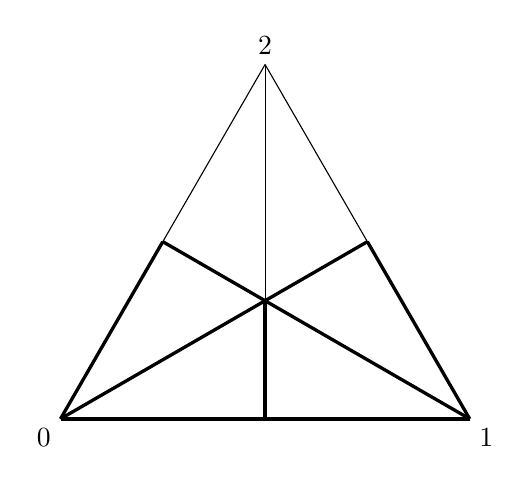
\begin{tikzpicture}

% Vertices of a triangle
\coordinate (2) at (90:3cm);
\coordinate (0) at (210:3cm);
\coordinate (1) at (-30:3cm);

% Nodes to mark vertices of a triangle
\node [above] at (2) {2};
\node [below left] at (0) {0};
\node [below right] at (1) {1};

% Draw line between the vertices 0,1 and 2 and name the midpoints
\draw (0.north east)--(2.south) coordinate[midway](02);
\draw [very thick] (0.north east)--(1.north west) coordinate[midway](01);
\draw (1.north west)--(2.south) coordinate[midway](12);

% Barycenter, could also be found by means of the intersection library of tikz
\coordinate (012) at (barycentric cs:0=1,1=1,2=1);

% Draws lines from vertices of original triangle to barycentre of original triangle and...
\draw [very thick] (0.north east)--(012) coordinate[midway](0<012);
\draw [very thick] (1.north west)--(012) coordinate[midway](1<012);
\draw (2.south)--(012) coordinate[midway](2<012);
\draw [very thick] (01)--(012) coordinate[midway](01<012);
\draw [very thick] (12)--(012) coordinate[midway](12<012); % Illustrate the cosieve
\draw [very thick] (02)--(012) coordinate[midway](02<012); % Illustrate the cosieve

% Illustrate the cosieve
\draw [very thick] (0.north east)--(02);
\draw [very thick] (1.north west)--(12);

\end{tikzpicture}
\caption{Nerve of the cosieve $W$}
\label{fig:Cosieve_in_subdivided_two_simplex_that_contains_second_edge}
\end{figure}

The pushout $Q\sqcup _PY^\sharp$ in $Cat$ is by the paragraph above taken along a Dwyer map, which implies that it is a poset \cite[Lem.~5.6.4]{Th80}. Furthermore, the pushout $W\sqcup _PY^\sharp$ in $Cat$ is a poset, say because it is taken along a rather trivial Dwyer map. Because $PoSet$ is a reflective subcategory of $Cat$ it follows that $W\sqcup _PY^\sharp$ can be considered a pushout in $PoSet$ of the underlying diagram.

Because $W=P\times [1]$, the pushout
\[T(B(\bar{y} ))=NW\sqcup _{NP}N(Y^\sharp )\]
in $sSet$ is the (backwards) topological mapping cylinder of $B(\bar{y} )$. Similarly,
\[M(B\bar{y} ))=N(W\sqcup _PY^\sharp )\]
is the (backwards) reduced mapping cylinder \cite[pp.~56--68]{WJR13}, which was defined in \cref{sec:intro}. Note that the canonical map
\[NW\sqcup _{NP}N(Y^\sharp )\to N(W\sqcup _PY^\sharp ),\]
is a guise of the cylinder reduction map $cr:T(B(\bar{y} ))\to M(B(\bar{y} ))$.

Next, consider the case when $X$ is generated by a single simplex. With the recognition made in the paragraph above, we are ready to discuss this case.
\begin{proposition}
\label{prop:t_X_iso_when_X_regular_gen_single_simplex}
Let $X$ be a regular simplicial set that is generated by a single simplex. Then $t_X$ is an isomorphism.
\end{proposition}
\begin{proof}
We will prove this by induction. Assume that $n>0$ is such that $t_X$ is an isomorphism for any regular $X$ that is generated by a non-degenerate simplex of degree $k<n$.

For the base step, one can note that the hypothesis holds for $n=1$ because $0$-dimensional simplicial sets are non-singular.

For the induction step, we assume that $X$ is as described in \cref{lem:second_reduction} and aim to prove that $t_X$ is an isomorphism. Notice that $Y$ is generated by the non-degenerate part of $y$, which is of degree $n-1$. This means that the assumption that $t_Y$ is an isomorphism, is justified.

\cref{lem:second_reduction} says that it suffices to prove that the map
\[D(NW\sqcup _{NP}N(Y^\sharp ))\to N(W\sqcup _PY^\sharp )\]
from Part $2$ is an isomorphism. In the text preceding this proof we saw that the latter map is a guise of the canonical map
\[dcr:DT(B(\bar{y} ))\to M(B(\bar{y} ))\]
whose source is the desingularized (backwards) topological mapping cylinder.

By \cref{thm:barratt_nerve_rep_map_dcr_iso}, the map $dcr$ is an isomorphism as $Y$ is regular.\\ \cref{lem:second_reduction} thus implies that $t_X$ is an isomorphism. This concludes the induction step.
\end{proof}
\noindent Note that \cref{prop:t_X_iso_when_X_regular_gen_single_simplex} relies upon \cref{thm:barratt_nerve_rep_map_dcr_iso}.

Now, recall \cref{lem:first_reduction}. We are ready to reduce \cref{thm:main_opt_triang} to \cref{thm:barratt_nerve_rep_map_dcr_iso}.
\begin{proof}[Proof of \cref{thm:main_opt_triang}.]
By \cref{prop:t_X_iso_when_X_regular_gen_single_simplex}, the assumption of \cref{lem:first_reduction} is satisfied. Thus we obtain \cref{thm:main_opt_triang}.
\end{proof}
\noindent Next, we keep our promise to explain the structure of the rest of this article.

Like the reader presumably have done so far, he preferably continues to read the sections in order, although there is a small detour in \cref{sec:cones}.

After \cref{sec:red}, which takes care of the deferred proof of \cref{lem:second_reduction}, we focus on \cref{thm:barratt_nerve_rep_map_dcr_iso} whose proof is rather technical. The work of proving \cref{thm:barratt_nerve_rep_map_dcr_iso} is divided into three tasks.

First, in \cref{sec:dzero}, we explain that
\[dcr:DT(B(\bar{y} ))\to M(B\bar{y} ))\]
is a bijection in degree $0$. This is a more or less formal argument involving not much more than the definition of the category $sSet$ as a set-valued functor category and the nerve functor.

Second, in \cref{sec:surject}, we show that $dcr$ is degreewise surjective. This is not trivial, however the answer is in our case more or less to be found in the pre-existing literature.

Third, in \cref{sec:zipping}, we do the part that seems hard to deduce from the literature, namely to prove that $dcr$ is degreewise injective in degrees above $0$. To do this, however, we separate out a few results in sections \ref{sec:tricat} and \ref{sec:deflation_thm}.

Finally, in \cref{sec:comparison}, we deduce \cref{thm:barratt_nerve_rep_map_dcr_iso} from the work of the three sections \ref{sec:dzero}, \ref{sec:surject} and \ref{sec:zipping}.

The reader may consider \cref{sec:cones} on cones as optional, as it is not really part of the storyline. On the other hand, it may yield insights into the idea behind the material in \cref{sec:zipping}. This is because the result presented in \cref{sec:cones} is a precursor. In addition, the reader may prefer our approach to the result stated as \cref{prop:cones_vs_mapping_cylinders} over any known proof.




\section{Reduction}
\label{sec:red}


This section is devoted to the proof of \cref{lem:second_reduction}. In the following proof we consider pushouts in four categories, namely the four objects in the commutative square
\begin{displaymath}
\xymatrix{
Cat \ar[r]^N & sSet \\
PoSet \ar[u]^U \ar[r]_N & nsSet \ar[u]_U
}
\end{displaymath}
of categories and functors.
\begin{proof}[Proof of \cref{lem:second_reduction} Part $1$.]
To factor the map $t_X$ in a useful way one can first factor $b_X:Sd\, X\to BX$ by means of the diagram
\begin{equation}
\label{eq:diagram_proof_lem_second_reduction}
\begin{gathered}
\xymatrix{
& Sd(\Delta [n]) \ar@{-}[d] \ar[dr] && Sd(\Delta [n-1]) \ar[ll]_{Sd(N\delta _n)} \ar@{-}[d] \ar[dr] \\
& \ar[d]_(.3)\cong ^(.3)b & Sd\, X \ar@/_6.3pc/[lldddd]_b \ar[dd]_(.65)f & \ar[d]_(.3)\cong ^(.3)b & Sd\, Y \ar[ll] \ar[dd] ^b \\
& B(\Delta [n]) \ar@/_/[lddd] \ar@/_/[dd] \ar[dr] & \ar[l] & B(\Delta [n-1]) \ar@{-}[l]_(.7){B(N\delta _n)} \ar[dr] \\
&& X' \ar[ld] && BY \ar@/^/[llld] \ar[ll] \ar@/^1pc/[lllldd] \\
& N(Q\sqcup _PY^\sharp ) \ar[ld] \\
BX
}
\end{gathered}
\end{equation}
where we have written the pushout $X'=NQ\sqcup _{NP}N(Y^\sharp )$ in $sSet$ of the lower square in the cube in (\ref{eq:diagram_proof_lem_second_reduction}) for brevity. The pushout $Q\sqcup _PY^\sharp$ is in $Cat$.

The functor $(-)^\sharp :sSet\to PoSet$ is cocontinous by \cref{lem:sharp_functor_preserves_colimits}. The pushout $Q\sqcup _PY^\sharp$ in $Cat$ is a poset \cite[Lem.~5.6.4]{Th80} as $P\to Q$ is a Dwyer map. Because $PoSet$ is a reflective subcategory of $Cat$ it then follows that the canonical map
\[Q\sqcup _PY^\sharp \xrightarrow{\cong } X^\sharp\]
is an isomorphism.

Naturality of $d_{Sd\, X}$ yields the diagram
\begin{displaymath}
\xymatrix{
Sd\, X \ar[d]_f \ar[r]^(.42)d & DSd(X) \ar[d]^{D(f)} \\
X' \ar[d]_{k} \ar[r]^(.47)d & DX' \ar@{-->}[ld]_(.53)l \ar[d]^{D(k)} \\
BX \ar[r]_(.45)d^(.45)\cong & DB(X)
}
\end{displaymath}
in which the diagonal map $l$ of the lower square arises due to the universal property of desingularization. It makes the upper left triangle of the lower square commute. Then the lower right triangle of the lower square commutes, also. This means we have a factorization of
\[b_X=k\circ f=l\circ d_{X'}\circ f=l\circ D(f)\circ d_{Sd\, X}\]
through $d_X$. The map $t_X$ is unique, so it follows that we get the useful factorization
\[t_X=l\circ D(f)\]
of the map $t_X$. The map $l$ is what we get when precomposing the canonical map
\[DX'\to N(Q \sqcup _PY^\sharp )\]
with the nerve of the canonical isomorphism
\[Q\sqcup _PY^\sharp \xrightarrow{\cong } X^\sharp .\]
Thus we see that $l$ is an isomorphism if $DX'\to N(Q \sqcup _PY^\sharp )$ is. We will see that $D(f)$ is an isomorphism, for formal reasons.

The map $D(f)$ is the canonical map between pushouts of $nsSet$ as $f$ is, by the universal property. It can be factored by applying the cocontinous functor $D$ to the diagram
\begin{displaymath}
\xymatrix@=1em{
Sd(\Delta [n-1]) \ar@/_5pc/[dddd]^b_\cong \ar[dd]_\cong ^d \ar[dr] \ar[rr] && Sd\, Y \ar@{-}[d] \ar[dr] \\
& Sd(\Delta [n]) \ar[dd]_(.6)\cong ^(.6)d \ar[rr] & \ar[d]^(.3)d & Sd\, X \ar[dd]_g \ar@/^2pc/[dddd]^f \\
DSd(\Delta [n-1]) \ar[dd]_\cong ^t \ar[dr] \ar@{-}[r] & \ar[r] & DSd\, Y \ar@{-}[d] \ar[dr] \\
& DSd(\Delta [n]) \ar[dd]_(.6)\cong ^(.6)t \ar[rr] & \ar[d]^(.3)t _(.3)\cong & X'' \ar[dd]_h \\
B(\Delta [n-1]) \ar[dr] \ar@{-}[r] & \ar[r] & BY \ar[dr] \\
& B(\Delta [n]) \ar[rr] && X'
}
\end{displaymath}
in $sSet$. The map $D(g)$ is an isomorphism because it is the canonical map between pushouts in $nsSet$ and because its source $DSd\, X$ and target $DX''$ are the most obvious ways of forming the pushout of the same diagram.

Recall from the formulation of the lemma that the map $t_Y$ is assumed to be an isomorphism. It follows that $D(h)$ is an isomorphism, hence $D(f)$ is an isomorphism. Hence, $t_X$ will be an isomorphism if $DX'\to N(Q\sqcup _PY^\sharp )$ is.
\end{proof}
\noindent We will conclude this section with the proof of Part $2$ of \cref{lem:second_reduction}.

The factorization $P\xrightarrow{i_0} W\xrightarrow{\psi } Q$ is through a cylinder $W=P\times [1]$. This coincidence means that we are dealing with mapping cylinders, although they play no explicit part in the rest of this section. What is relevant here, in the proof of Part $2$ of \cref{lem:second_reduction}, is the somewhat more general phenomenon of taking pushouts along the nerve of a Dwyer map.

As mapping cylinders are important technical tools it is an interesting problem in its own right to find interesting conditions under which the desingularized topological mapping cylinder is the reduced one. The work of \cref{sec:zipping} is a contribution to this end. When dealing with mapping cylinders of the nerve of a map between posets, Dwyer maps are always lurking in the background.

We are ready to prove Part $2$ of \cref{lem:second_reduction}, and thus completing the proof.
\begin{proof}[Proof of \cref{lem:second_reduction} Part $2$.]
The result follows immediately from \cref{prop:pushout_along_Dwyer} when we let
\begin{displaymath}
\begin{array}{rcl}
j\circ i & = & (N\delta _n)^\sharp \\
\varphi & = & (\bar{y} )^\sharp .
\end{array}
\end{displaymath}
In particular, $R=Y^\sharp$.
\end{proof}
\noindent Note that \cref{prop:pushout_along_Dwyer} slightly generalizes Part $2$ of \cref{lem:second_reduction}, but keeps the notation.

The next proposition is proven, essentially by using a technique by Thomason \cite[p.~316]{Th80} in his proof of Proposition 4.3 \cref{prop:pushout_along_Dwyer}.
\begin{proposition}\label{prop:pushout_along_Dwyer}
Let
\begin{displaymath}
\xymatrix{
NP \ar[d] \ar[r] & NR \ar[d] \\
NQ \ar[r] & NQ\sqcup _{NP}NR
}
\end{displaymath}
be a cocartesian square in $sSet$ where $P$, $Q$ and $R$ are posets and where $P\to Q$ is a Dwyer map with factorization $P\to W\to Q$. Then the map
\[D(NQ\sqcup _{NP}NR)\to N(Q\sqcup _PR)\]
is an isomorphism if
\[D(NW\sqcup _{NP}NR)\to N(W\sqcup _PR)\]
is an isomorphism.
\end{proposition}
\noindent By stating \cref{prop:pushout_along_Dwyer}, we have freed ourselves of the specific objects involved in \cref{lem:second_reduction}.

To tie together the studies of the two maps of \cref{prop:pushout_along_Dwyer} we consider the diagram
\begin{equation}
\label{eq:diagram_proof_prop_pushout_along_Dwyer}
\begin{gathered}
\xymatrix@C=0.5em@R=0.8em{
NP \ar[dd]^{Ni} \ar[dr] \ar[rr]^{N\varphi } && NR \ar@{-}[d] \ar[dr] \\
& NR \ar[dd] & \ar[d] & NR \ar[ll] \ar[dd] \\
NW \ar[dd]^{Nj} \ar[dr] \ar@{-}[r] & \ar[r] & NW\sqcup _{NP}NR \ar@{-}[d] \ar[dr]^\eta \\
& N(W\sqcup _PR) \ar[dd] & \ar[d] & D(NW\sqcup _{NP}NR) \ar[ll]_\zeta \ar[dd] \ar@/^6.5pc/[dddd] \\
NQ \ar[dr] \ar@{-}[r] & \ar[r] & NQ\sqcup _{NP}NR \ar@{-}@/_/[d] \ar[dr]^{\bar{\eta } } \\
& N(Q\sqcup _PR) & \ar@/_1pc/[ddr]^\eta & NQ\sqcup _{NW}D(NW\sqcup _{NP}NR) \ar[ll]_{\bar{\zeta }} \ar@{-->}[dd]_\xi \\
\\
&&& D(NQ\sqcup _{NP}NR) \ar@/^1pc/[lluu]^{\hat{\zeta } }
}
\end{gathered}
\end{equation}
in $sSet$. We take (\ref{eq:diagram_proof_prop_pushout_along_Dwyer}) as a naming scheme for the maps that play a role in the argument. Note that $\zeta$ is the map
\[dcr:DT(N\varphi )\to M(N\varphi )\]
in the case when $W=P\times [1]$ and when the map $i:P\to W$ is the map $p\mapsto (p,0)$.
\begin{proof}[Proof of \cref{prop:pushout_along_Dwyer}.]
By \cref{lem:proof_of_second_reduction}, the map $\hat{\zeta }$ is a cobase change in $sSet$ of $\zeta$. This means that $\hat{\zeta }$ is epic if $\zeta$ is. The epics of $sSet$ are precisely the degreewise surjective maps. Furthermore, a cobase change in $sSet$ of a degreewise injective map is again degreewise injective. This way we get that $\hat{\zeta }$ is an isomorphism if $\zeta$ is.
\end{proof}
\noindent Notice that \cref{prop:pushout_along_Dwyer} relies upon the following.
\begin{lemma}\label{lem:proof_of_second_reduction}
The map $\hat{\zeta }$ is a cobase change in $sSet$ of $\zeta$.
\end{lemma}
\begin{proof}
We will prove that $\hat{\zeta }$ is the cobase change in $sSet$ of $\zeta$ along
\[D(NW\sqcup _{NP}NR)\to D(NQ\sqcup _{NP}NR).\]
It suffices to prove that
\begin{equation}
\label{eq:first_diagram_lem_proof_of_second_reduction}
\begin{gathered}
\xymatrix{
NW \ar[d]_{Nj} \ar[r] & N(W\sqcup _PR) \ar[d] \\
NQ \ar[r] & N(Q\sqcup _PR)
}
\end{gathered}
\end{equation}
is cocartesian in $sSet$ and that $\xi$ is an isomorphism.

Let $V$ be the full subposet of $Q$ whose objects are those that are not in $P$. Then $V$ is a cosieve in $Q$ as $P$ is sieve. The square (\ref{eq:first_diagram_lem_proof_of_second_reduction}) fits into the bigger diagram
\begin{equation}
\label{eq:second_diagram_lem_proof_of_second_reduction}
\begin{gathered}
\xymatrix{
& NW \ar@{-}[d] \ar[dr] \\
NV\cap NW=N(V\cap W) \ar[dd] \ar[ur] \ar[rr] & \ar[d]^(.35){Nj} & N(W\sqcup _PR) \ar[dd] \\
& NQ \ar[dr] \\
NV \ar[rr] \ar[ur] && N(Q\sqcup _PR)
}
\end{gathered}
\end{equation}
where the cosieve $V$ in $Q$ makes an appearance.

The maps $V\cap W\to V$ and $V\cap W\to W$ are cosieves, so it follows that $Q$ can be decomposed as a pushout
\[Q\cong V\sqcup _{V\cap W}W\]
in $Cat$. Observe that $V\cap W\to W\sqcup _PR$ is also a cosieve. It follows that $N:Cat\to sSet$ preserves the pushouts $Q$ and
\[Q\sqcup _PR\cong V\sqcup _{V\cap W}(W\sqcup _PR).\]
From the diagram (\ref{eq:second_diagram_lem_proof_of_second_reduction}) we now see that (\ref{eq:first_diagram_lem_proof_of_second_reduction}) is cocartesian. From (\ref{eq:diagram_proof_prop_pushout_along_Dwyer}) we verify that $\bar{\zeta }$ is the cobase change in $sSet$ of $\zeta$ along
\[D(NW\sqcup _{NP}NR)\to NQ\sqcup _{NW}D(NW\sqcup _{NP}NR).\]
It remains to argue that $\xi$ is an isomorphism.

The nerve of the cosieve
\[V\cap W\to W\sqcup _PR\]
factors through
\[NV\cap NW\to D(NW\sqcup _{NP}NR),\]
so the latter is degreewise injective. Therefore
\[NQ\sqcup _{NW}D(NW\sqcup _{NP}NR)\cong NV\sqcup _{NV\cap NW}D(NW\sqcup _{NP}NR)\]
is non-singular.

The map
\[\eta :NQ\sqcup _{NP}NR\to D(NQ\sqcup _{NP}NR)\]
is degreewise surjective, therefore $\xi$ is. As the source of $\xi$ is non-singular, the map is an isomorphism.
\end{proof}








\section{Degree zero}
\label{sec:dzero}


We make use of the following result. Let $Cat$ denote the category of small categories.
\begin{lemma}\label{lem:degree_zero_colimit_category_nerve}
Let $F:J\to Cat$ be a functor whose source is a small category. Let $\mathscr{L}$ be the colimit of $F$. If $X$ is the colimit of the composite diagram
\[J\xrightarrow{F} Cat\xrightarrow{N} sSet,\]
then the canonical map $X\to N\mathscr{L}$ is a bijection in degree $0$.
\end{lemma}
\begin{proof}
Let $O$ denote the functor $Cat\to Set$ that takes a small category to the set of its objects. Recall that $O$ has a right adjoint, namely the functor that takes a set $S$ to the indiscrete category $IS$. This is the category whose set of objects is precisely $S$ and that is such that each hom set is a singleton.

We also use the functor
\[sSet=Fun(\Delta ^{op},Set)\xrightarrow{(-)_0} Set\]
that sends a simplicial set to the set of its $0$-simplices. There is a natural bijection
\[O\mathscr{C} \xrightarrow{\cong} (N\mathscr{C} )_0,\]
that takes an element $c$ of the set $O\mathscr{C}$ of objects of a small category $\mathscr{C}$ to the simplex $[0]\to \mathscr{C}$ with $0\mapsto c$.

Because $O$ is cocontinous, we get a canonical function $O\mathscr{L} \to X_0$. As colimits in $sSet$ are formed degreewise it follows that this function is a bijection. There is also a canonical function $O\mathscr{L} \to (N\mathscr{L} )_0$, which by naturality must be the mentioned bijection. The induced map $X_0\to (N\mathscr{L} )_0$ fits into a triangle
\begin{displaymath}
\xymatrix{
O\mathscr{L} \ar[dr]_\cong \ar[rr]^\cong && (N\mathscr{L} )_0 \\
& X_0 \ar[ur] \\
}
\end{displaymath}
that commutes by the universal property of the colimit $O\mathscr{L}$. Hence, our claim that $X\to N\mathscr{L}$ is a bijection in degree $0$ is true.
\end{proof}
\noindent An application of the previous lemma is the following example.
\begin{example}\label{ex:pushout_poset_along_dwyer}
Let $F':J\to PoSet$ be a diagram
\begin{displaymath}
\xymatrix{
P \ar[d]_k \ar[r]^\varphi & R \\
Q
}
\end{displaymath}
where $k$ is a Dwyer map. As $PoSet$ is a reflective subcategory of $Cat$, it follows that $U:PoSet\to Cat$ preserves the pushout of $F'$ \cite[Lem.~5.6.4]{Th80}. If $Q\sqcup _PR$ is the colimit of $F=U\circ F'$, then \cref{lem:degree_zero_colimit_category_nerve} says that
the canonical map
\[NQ\sqcup _{NP}NR\to N(Q\sqcup _PR)\]
is a bijection in degree $0$.

In particular, if $k$ is the special Dwyer map
\[k=i_0:P\to P\times [1]=Q,\]
then the reduction map
\[cr:T(N\varphi )\to M(N\varphi )\]
is in general a bijection in degree $0$.
\end{example}



\section{Tricategorical comparison}
\label{sec:tricat}

Often, one compares pushouts taken in several different subcategories. For example, in this article, we are interested in the commutative triangle
\begin{equation}
\label{eq:first_diagram_proof_prop_barratt_nerve_rep_map_dcr_inj}
\begin{gathered}
\xymatrix@=1em{
T(N\varphi ) \ar[dr]_{cr} \ar[rr]^{\eta } && DT(N\varphi ) \ar[ld]^{dcr} \\
& M(N\varphi )
}
\end{gathered}
\end{equation}
that factors the cylinder reduction map through the canonical degreewise surjective map $\eta$ whose target is the desingularization of the topological mapping cylinder.

To study $dcr$ is for many purposes to study $\eta$ and $cr$. There is a condition on
\[\eta _{T(N\varphi )}:T(N\varphi )\to DT(N\varphi )\]
that will ensure that $dcr$ is degreewise injective.
\begin{definition}
\label{def:siblings}
Whenever $x$ and $x'$ are simplices of the same degree of some simplicial set, we will say that they are \textbf{siblings} if $x\varepsilon _j=x'\varepsilon _j$ for all $j$.
\end{definition}
\noindent Our motivating example for the next result is $f=\eta _{T(N\varphi )}$, $g=dcr$ and $h=cr$.
\begin{proposition}\label{prop:criterion_degreewise_injective_into_nerve_computation}
Suppose we have a commutative diagram
\begin{displaymath}
\xymatrix{
X \ar[dr]_h \ar[rr]^f && Y \ar[ld]^g \\
& Z
}
\end{displaymath}
in $sSet$ in which $f$ is degreewise surjective and
\[h_0:X_0\to Z_0\]
is injective. Furthermore, assume that $Y$ is non-singular and that $Z$ is the nerve
of some poset. The simplicial map $g$ is injective in a given degree $q>0$ if and only if
\[f(x)=f(x')\]
whenever $x$ and $x'$ are embedded siblings of degree $q$.
\end{proposition}
\noindent Before we prove the proposition, we remind the reader of some standard piece of terminology.

Recall the Eilenberg-Zilber lemma \cite[Thm.~4.2.3]{FP90}, which says that each simplex $x$ of each simplicial set is uniquely a degeneration $x=x^\sharp x^\flat$ of a non-degenerate simplex. The non-degenerate simplex $x^\sharp$ is the \textbf{non-degenerate part} of $x$ and $x^\flat$ is the \textbf{degenerate part}.
\begin{proof}[Proof of \cref{prop:criterion_degreewise_injective_into_nerve_computation}.]
The ``only if'' part will not be needed, but we state it to emphasize that the conditions are equivalent under the hypothesis of the lemma. This part uses that the diagram commutes and that $Z$ is the nerve of a poset.

Suppose $g$ is injective in degree $q$ and that $x$ and $x'$ are siblings of degree $q$. Then
\[h(x)\varepsilon _j=h(x\varepsilon _j)=h(x'\varepsilon _j)=h(x')\varepsilon _j\]
for each $j$, so $h(x)$ and $h(x')$ are siblings. This implies that $h(x)=h(x')$ as $Z$ is the nerve of a poset. Because the diagram commutes and because $g$ is injective in degree $q$, it follows that $f(x)=f(x')$.

To prove the ``if'' part, we will use every condition of the hypothesis of the lemma, except that $Z$ is the nerve of a poset. First, observe that $g_0$ is injective as $h_0$ is injective and as $f_0$ is surjective and hence a bijection.

Suppose $f$ satisfies the described condition and that $y_1$ and $y_2$ are simplices of $Y$, of degree $q$, such that
\begin{equation}\label{lb:Equation0_criterion_embedded_sieblings}
g(y_1)=g(y_2).
\end{equation}
We prove that $y_1=y_2$, which will imply that $g$ is injective in degree $q$. This we do by proving that the non-degenerate parts and the degenerate parts of $y_1$ and $y_2$ are equal, respectively.

The two decompositions
\begin{displaymath}
g(y_1)=g(y_1)^\sharp g(y_1)^\flat
\end{displaymath}
\begin{displaymath}
g(y_1)=g(y_1^\sharp y_1^\flat )=g(y_1^\sharp )y_1^\flat =g(y_1^\sharp )^\sharp g(y_1^\sharp )^\flat y_1^\flat .
\end{displaymath}
are one and the same due to the uniqueness part of the Eilenberg-Zilber lemma.

As usual, then, we have the equations
\begin{equation}\label{lb:Equation1_criterion_embedded_sieblings}
g(y_1)^\sharp =g(y_1^\sharp )^\sharp
\end{equation}
\begin{equation}\label{lb:Equation2_criterion_embedded_sieblings}
g(y_1)^\flat =g(y_1^\sharp )^\flat y_1^\flat .
\end{equation}
However, because $Y$ is non-singular, the non-degenerate simplex $y_1^\sharp$ is embedded, which is the same as saying that its vertices are pairwise distinct. Because $g$ is injective in degree $0$ it follows that $g(y_1^\sharp )=g(y_1^\sharp )^\sharp$ is embedded and thus non-degenerate. This implies that (\ref{lb:Equation1_criterion_embedded_sieblings}) turns into
\begin{equation}\label{lb:Equation3_criterion_embedded_sieblings}
g(y_1)^\sharp =g(y_1^\sharp ).
\end{equation}
That $g(y_1^\sharp )$ is non-degenerate also implies that the degeneracy operator $g(y_1^\sharp )^\flat$ is the identity, meaning (\ref{lb:Equation2_criterion_embedded_sieblings}) turns into
\begin{equation}\label{lb:Equation4_criterion_embedded_sieblings}
g(y_1)^\flat =y_1^\flat .
\end{equation}
The reasoning we applied to $y_1$ is equally valid for $y_2$, so
\begin{equation}\label{lb:Equation5_criterion_embedded_sieblings}
g(y_2)^\sharp =g(y_2^\sharp )
\end{equation}
\begin{equation}\label{lb:Equation6_criterion_embedded_sieblings}
g(y_2)^\flat =y_2^\flat .
\end{equation}

Due to the assumption (\ref{lb:Equation0_criterion_embedded_sieblings}) the combination of (\ref{lb:Equation3_criterion_embedded_sieblings}) and (\ref{lb:Equation5_criterion_embedded_sieblings}) yields
\begin{equation}\label{lb:Equation7_criterion_embedded_sieblings}
g(y_1^\sharp )=g(y_2^\sharp )
\end{equation}
by the uniqueness part of the Eilenberg-Zilber lemma, again. For the same reason, the combination of (\ref{lb:Equation4_criterion_embedded_sieblings}) and (\ref{lb:Equation6_criterion_embedded_sieblings}) yields
\begin{equation}\label{lb:Equation8_criterion_embedded_sieblings}
y_1^\flat =y_2^\flat .
\end{equation}
Thus we get that the degenerate part of $y_1$ is equal to the degenerate part of $y_2$. It remains to prove that $y_1$ and $y_2$ have the same non-degenerate part.

Suppose $y_1^\sharp =f(x_1)$ and $y_2^\sharp =f(x_2)$. Such simplices $x_1$ and $x_2$ exist as $f$ is degreewise surjective, and they are embedded in $X$ as $y_1^\sharp$ and $y_2^\sharp$ are embedded in $Y$. Due to (\ref{lb:Equation7_criterion_embedded_sieblings}) we know that $h(x_1)=h(x_2)$, hence
\[h(x_1\varepsilon _j)=h(x_1)\varepsilon _j=h(x_2)\varepsilon _j=h(x_2\varepsilon _j)\]
for each $j$. As $h$ is injective in degree $0$ it follows that $x_1$ and $x_2$ are siblings. Finally, as $f$ sends embedded siblings to the same simplex, we get
\begin{equation}\label{lb:Equation9_criterion_embedded_sieblings}
y_1^\sharp =f(x_1)=f(x_2)=y_2^\sharp .
\end{equation}
Now we also know that the non-degenerate part of $y_1$ is equal to the non-degenerate part of $y_2$.

The equations (\ref{lb:Equation8_criterion_embedded_sieblings}) and (\ref{lb:Equation9_criterion_embedded_sieblings}) together imply that $y_1=y_2$, so it follows that $g$ is injective in degree $q$.
\end{proof}




\section{Concerning cones}
\label{sec:cones}


There is an interesting result concerning mapping cylinders that is related to \cref{thm:barratt_nerve_rep_map_dcr_iso}, namely \cref{prop:cones_vs_mapping_cylinders} below.

A possible proof of \cref{prop:cones_vs_mapping_cylinders} was an inspiration for \cref{thm:barratt_nerve_rep_map_dcr_iso}, so this section should also give the reader insight into the idea behind the proof of \cref{thm:barratt_nerve_rep_map_dcr_iso} and the proof by induction presented in \cref{sec:zipping}.

The result says the following.
\begin{proposition}
\label{prop:cones_vs_mapping_cylinders}
Let $P$ be some poset. Then the canonical map $dcr$ in the diagram
\begin{displaymath}
\xymatrix{
NP \ar[d]_{i_0} \ar[r]^{N\varphi } & \Delta [0] \ar[d] \ar@/^1.5pc/[ddr] \\
NP\times \Delta [1] \ar@/_1pc/[drr] \ar[r] & DT(N\varphi ) \ar[dr]^{dcr} \\
&& M(N\varphi )
}
\end{displaymath}
in $nsSet$ is an isomorphism.
\end{proposition}
\noindent In words, \cref{prop:cones_vs_mapping_cylinders} says that the desingularization of the cone on $NP$ is the reduced mapping cylinder of the unique map $NP\to \Delta [0]$.
\begin{proof}[Proof of \cref{prop:cones_vs_mapping_cylinders}.]
We will argue that $dcr$ is degreewise surjective, that it is a bijection in degree $0$ and finally that it is injective in degrees above $0$.

Let $k$ denote $i_0:P\to P\times[1]$ as in \cref{ex:pushout_poset_along_dwyer}. Then $k$ is canonically identified with $i_0:NP\to NP\times \Delta [1]$. Let $\bar{\varphi }$ denote the cobase change (in the category of posets) of $\varphi$ along $k$ and let $\bar{k}$ denote the cobase change of $k$ along $\varphi$. The map $k$ is a special kind of Dwyer map. Furthermore, let $r:P\times [1]\to P$ be the projection onto the first factor.

First, the map
\[cr:T(N\varphi )\to M(N\varphi )\]
is degreewise surjective in this special case, as we now explain. This immediately implies that $dcr$ is degreewise surjective.

If $z:[q]\to P\times [1]\sqcup _{P}[0]$ is some simplex in
\[M(N\varphi )=N(P\times [1]\sqcup _{P}[0]),\]
then there is some integer $j$ with $-1\leq j\leq q$ that has the property that $z(i)$ is in the image of $k$ for $i\leq j$ and that $z(i)$ is not in the image of $k$ for $i>j$. There is a $q$-simplex $x'$ of $T(N\varphi )$ whose image under $cr$ is $z$. It is defined thus.

If $j=q$, then we can simply define $x'$ as a degeneracy of the unique $0$-simplex that is in the image of $\Delta [0]\to T(N\varphi )$. Else if $j<q$, then we may for each $i>j$ define $x(i)$ as the uniqe element of $P\times [1]$ that $\bar{\varphi }$ sends to $z(i)$. Suppose
\[\bar{\varphi } (p,1)=z(j+1).\]
For each $i\leq j$, we define $x(i)=(p,1)$. Let $x'$ be the image of $x$ under $NP\times \Delta [1]\to T(N\varphi )$. It follows that $cr(x')=z$. This finishes the argument that $cr$ is degreewise surjective, and therefore that $dcr$ is. Keep in mind that $cr$ and $dcr$ fit into the commutative triangle (\ref{eq:first_diagram_proof_prop_barratt_nerve_rep_map_dcr_inj}).

By \cref{ex:pushout_poset_along_dwyer}, the map $cr$ is a bijection in degree $0$, which by (\ref{eq:first_diagram_proof_prop_barratt_nerve_rep_map_dcr_inj}) implies that $dcr$ is. It remains to verify that $dcr$ is injective in degrees above $0$.

For the argument that $dcr$ is degreewise injective in degrees above $0$, we will apply \cref{prop:criterion_degreewise_injective_into_nerve_computation} to (\ref{eq:first_diagram_proof_prop_barratt_nerve_rep_map_dcr_inj}).

Consider embedded siblings $x'$ and $y'$ of $T(N\varphi )$, say of degree $q>0$, whose zeroth common vertex is in the image of $\Delta [0]\to T(N\varphi )$ and whose $q$-th common vertex is not. This is the only non-trivial case. Let $x$ and $y$, respectively, be the unique simplices in $NP\times \Delta [1]$ whose image under $NP\times \Delta [1]\to T(N\varphi )$ is $x'$ and $y'$. Because the target of $\varphi$ has only one element, we see from (\ref{eq:first_diagram_proof_prop_cones_vs_mapping_cylinders}) that $\eta (x')=\eta (y')$.
\begin{equation}
\label{eq:first_diagram_proof_prop_cones_vs_mapping_cylinders}
\begin{gathered}
\xymatrix{
x(0) \ar[dr] \ar@{-->}[r] & kr(x(1)) \ar@{-->}[d] & y(0) \ar[ld] \ar@{-->}[l] \\
& x(1)=y(1) \ar[d] \\
& \dots \ar[d] \\
& x(q)=y(q)
}
\end{gathered}
\end{equation}
By \cref{prop:criterion_degreewise_injective_into_nerve_computation}, it follows that $dcr$ is injective in degree $q$. This finishes the proof that $dcr$ is injective in degrees above $0$ and hence an isomorphism.
\end{proof}





\section{Surjectivity of the cylinder reduction}
\label{sec:surject}

Not every cylinder reduction map
\[cr:T(N\varphi )\to M(N\varphi )\]
is degreewise surjective. It can happen that the dimension of the reduced mapping cylinder is strictly higher than the dimension of the topological mapping cylinder.
\begin{example}\label{ex:Non-surjective_cylinder_reduction}
Let $\varphi :P\to R$ be the functor between posets defined as follows. Its source is the poset
\[P=\{ b\leftarrow a\rightarrow c\}\]
and its target is the poset
\[R=\{ a'\rightarrow b'\rightarrow c'\} .\]
The functor is given on objects by $\varphi (a)=a'$, $\varphi (b)=b'$ and $\varphi (c)=c'$.

The (backwards) topological mapping cylinder $T(N\varphi )$ is evidently of dimension $2$. However, the (backwards) reduced mapping cylinder $M(N\varphi )$ is by definition the nerve of the pushout of the diagram
\begin{displaymath}
\xymatrix{
P \ar[d]_{i_0} \ar[r]^\varphi & R \\
P\times [1]
}
\end{displaymath}
in $PoSet$. Thus the reduced mapping cylinder is seen to be of dimension $3$, so the cylinder reduction map is not surjective in degree $3$.
\end{example}
\noindent Note that, in \cref{ex:Non-surjective_cylinder_reduction}, the image of $\varphi$, meaning the smallest subcategory of $R$ containing each object and each morphism hit by $\varphi$, is not a sieve in $R$. This is because the morphism $b'\to c'$ is not in the image of $\varphi$, though the object $c'$ is.

To take care of the surjectivity statement of \cref{thm:barratt_nerve_rep_map_dcr_iso}, we will adapt Lemma $2.5.6$ from \cite[p.~71]{WJR13} to our needs. Recall from \cref{def:simple_map_calculating_dsd2} the notion of simple maps. Note that a simple map is degreewise surjective. Simple maps are discussed in Chapter $2$ of \cite[pp.~29--97]{WJR13} and play a role in that book.

Let $f:X\to Y$ be a simplicial map whose source $X$ is a finite simplicial set. We say that $f$ is \textbf{simple onto its image} if the induced map $X\to f(X)$ is simple.
\begin{lemma}{(Lemma $2.5.6$ of \cite[p.~71]{WJR13})}
\label{lem:barrat_nerve_of_any_representing_map_of_regular_simple}
Let $X$ be a regular simplicial set. For each $n\geq 0$ and for each $n$-simplex $y$, the map
\[B(\bar{y} ):B(\Delta [n])\to BX\]
induced by the representing map $\bar{y}$ is simple onto its image.
\end{lemma}
\noindent Note that if $Y$ is the image of the representing map $\bar{y}$ of some simplex $y$, then $BY$ is the image of $B(\bar{y} )$ \cite[Lem.~2.4.20,~p.~67]{WJR13}.

In the rather lengthy proof of \cref{lem:barrat_nerve_of_any_representing_map_of_regular_simple}, which we display below, the following term from \cite[Def.~2.4.7]{WJR13} is an ingredient.
\begin{definition}
\label{def:simplicial_homotopy_equivalence_over_the_target}
Let $X$ and $Y$ be finite simplicial sets. A map $f:X\to Y$ is a \textbf{simplicial homotopy equivalence over the target} if there is a section $s:Y\to X$ of $f$ and a simplicial homotopy $H$ between $s\circ f$ and the identity $X\to X$ such that the square
\begin{displaymath}
\xymatrix{
X\times \Delta [1] \ar[d]_{pr_1} \ar[r]^(.6)H & X \ar[d]^f \\
X \ar[r]_f & Y
}
\end{displaymath}
commutes.
\end{definition}
\noindent Note that the homotopy $H$ provides a contraction of each point inverse of $\lvert f\rvert$, so $f$ is simple. There are several related notions that could fill the term of \cref{def:simplicial_homotopy_equivalence_over_the_target} \cite[p.~60]{WJR13} with meaning.

We are ready to prove the lemma.
\begin{proof}[Proof of \cref{lem:barrat_nerve_of_any_representing_map_of_regular_simple}.]
The proof is borrowed from the corresponding part of the proof of Lemma 2.5.6 from \cite[p.~71]{WJR13}. The only difference is that the notion of op-regularity is replaced with regularity.

Notice that it is enough to consider the representing maps of non-degenerate simplices. If $y$ is a simplex of $X$, say of degree $n$, then we can factor $B(\bar{y} )$ as
\[B(\Delta [n])\xrightarrow{B(Ny^\flat )} B(\Delta [k])\xrightarrow{B(\overline{y^\sharp } )} BX\]
where $k$ denotes the degree of $\bar{y}$ and where $B(Ny^\flat )$ is simple as it is a simplicial homotopy equivalence over the target.

Assume that $n>0$ is an integer such that the representing map of each non-degenerate simplex of $X$, of degree strictly less than $n$, is simple onto its image. Assume that $y$ is a non-degenerate simplex of degree $n$. We will prove that $B(\bar{y} )$ is simple onto its image.

Let $z=y\delta _n$ so that the image $Y$ of $\bar{y}$ is a pushout $\Delta [n]\sqcup _{\Delta [n-1]}Z$, where $Z$ is the image of $\bar{z} :\Delta [n-1]\to X$. Here, $\Delta [n]$ is attached to $Z$ along its $n$-th face, meaning along the map $N\delta _n$.

By the induction hypothesis, the map
\[B(\bar{z} ):B(\Delta [n-1])\to BX\]
is simple onto its image as the degree of $z^\sharp$ is at most $n-1$. The simplicial subset $BZ$ of $BX$ is the image of the Barratt nerve of the representing map of $z$ \cite[Lem.~2.4.20]{WJR13}.

In \cref{fig:Cosieve_in_subdivided_two_simplex_that_contains_second_edge} we displayed the simplicial set $B(\Delta [2])$ and highlighted a copy of $B(\Delta [1])\times \Delta [1]$ as a simplicial subset. The figure holds the key to a decomposition
\[B(\Delta [n])\cong M(B(\Delta [n-1])\to \Delta [0])\sqcup _{B(\Delta [n-1])}B(\Delta [n-1])\times \Delta [1]\]
as we now explain.

Recall the embedding $\psi :\Delta [n-1]^\sharp \times [1]\to \Delta [n]^\sharp$ from the proof of \cref{lem:second_reduction}. Form the backwards reduced mapping cylinder
\[M(B(\Delta [n-1])\to \Delta [0])\]
of $B(\Delta [n-1])\to \Delta [0]$. This mapping cylinder is the nerve of the pushout $P(\Delta [n-1]^\sharp \to [0])$ of
\begin{displaymath}
\xymatrix{
\Delta [n-1]^\sharp \ar[d]_{i_0} \ar[r] & [0] \\
\Delta [n-1]^\sharp \times [1]
}
\end{displaymath}
where $i_0$ takes $\mu$ to $(\mu ,0)$. The cosieve
\[i_1:\Delta [n-1]^\sharp \to \Delta [n-1]^\sharp \times [1]\]
gives rise to a cosieve
\[\Delta [n-1]^\sharp \to P(\Delta [n-1]^\sharp \to [0]).\]

Furthermore, we can define a map
\[\omega :\Delta [n-1]^\sharp \times [1]\to \Delta [n]^\sharp\]
by letting it send $(\mu ,0)$ to $\varepsilon _n$ and $(\mu :[m]\to [n-1],1)$ to the operator
\[[m+1]\to [n]\]
given by $j\mapsto \mu (j)$ for $0\leq j\leq m$ and $m+1\mapsto n$. From $\omega$ arises the right hand vertical map of the commutative square
\begin{displaymath}
\xymatrix{
\Delta [n-1]^\sharp \ar[d]_{i_1} \ar[r] & P(\Delta [n-1]^\sharp \to [0]) \ar[d] \\
\Delta [n-1]^\sharp \times [1] \ar[r]_(.6)\psi & \Delta [n]^\sharp
}
\end{displaymath}
which is cocartesian in the category of posets and even in the category of small categories. Moreover, the nerve functor preserves it as a cocartesian square as the legs are cosieves. This concludes the argument that $B(\Delta [n])$ can be decomposed as claimed.

Next, we display a suitable decomposition of $BY$. Form the backwards mapping cylinder $M(B(\bar{z} ))$ of the Barratt nerve of the corestriction to $Z$ of the representing map of the simplex $z$. Here, we overload the symbol $\bar{z}$. There is a degreewise injective map
\[B(\Delta [n-1])\xrightarrow{i_1} B(\Delta [n-1])\times \Delta [1]\to M(B(\bar{z} ))=NP((\bar{z} )^\sharp ),\]
which is induced by
\[\Delta [n-1]^\sharp \xrightarrow{i_1} \Delta [n-1]^\sharp \times [1]\to P((\bar{z} )^\sharp ).\]
As the simplicial set $Y$ is regular, the composite
\[P(\Delta [n-1]^\sharp \to [0])\to \Delta [n]^\sharp \xrightarrow{(\bar{y} )^\sharp } Y^\sharp\]
is injective on objects and actually a cosieve.

Next, consider the pushout
\[Y^\sharp =\Delta [n]^\sharp \sqcup _{\Delta [n-1]^\sharp }Z^\sharp .\]
Use the factorization of $(N\delta _n)^\sharp$ into $\psi \circ i_0$ as before and obtain $P((\bar{z} )^\sharp )\to Y^\sharp$ written as the cobase change of $\psi$ along $\Delta [n-1]^\sharp \times [1]\to P((\bar{z} )^\sharp )$. Combining this with the decomposition of $\Delta [n]^\sharp$ obtained above, we get the cocartesian square
\begin{displaymath}
\xymatrix{
\Delta [n-1]^\sharp \ar[d] \ar[r] & P(\Delta [n-1]^\sharp \to [0]) \ar[d] \\
P((\bar{z} )^\sharp ) \ar[r] & Y^\sharp
}
\end{displaymath}
which is also preserved by the nerve. Again, this is because both legs are cosieves. The diagram
\begin{displaymath}
\xymatrix{
B(\Delta [n-1])\times \Delta [1] \ar[d] & B(\Delta [n-1]) \ar[l]_(.4){i_1} \ar[d]^{id} \ar[r] & M(B(\Delta [n-1])\to \Delta [0]) \ar[d]^{id} \\
M(B(\bar{z} )) & B(\Delta [n-1]) \ar[l] \ar[r] & M(B(\Delta [n-1])\to \Delta [0])
}
\end{displaymath}
is a thus a way of obtaining the map $B(\Delta [n])\to BY$ induced by $B(\bar{y} )$.

On the cone $M(B(\Delta [n-1])\to \Delta [0])$, the map $B(\bar{y})$ is the identity. However, on the cylinder $B(\Delta [n-1])\times \Delta [1]$, the map $B(\bar{y})$ is the composite
\[B(\Delta [n-1])\times \Delta [1]\to T(B(\bar{z} ))\to M(B(\bar{z} )).\]

The first map of the composite above is the cobase change of the simple map $B(\bar{z} )$ along $i_0$. A point inverse of that map is either a point inverse under the induced map
\[\lvert B(\Delta [n-1])\rvert \times \lvert \Delta [1]\rvert -\lvert B(\Delta [n-1])\rvert \xrightarrow{\cong } \lvert T(B(\bar{z} )\rvert -\lvert BZ\rvert ,\]
which is a homeomorphism, or it can be considered a point inverse under
\[\lvert B(\bar{z} )\rvert :\lvert B(\Delta [n-1])\rvert \to  BZ.\]
Thus the first map of the composite is simple.

The second map is simple by the induction hypothesis and by Lemma 2.4.21. \cite[p.~67]{WJR13} as $\Delta [n-1]$ and $Z$ are of strictly lower dimension than $n$.
\end{proof}
\noindent Thus we obtain the technically important fact that for a regular simplicial set, the Barratt nerve of each representing map is simple onto its image.

We use the following notion from \cite[Def.~2.4.9]{WJR13}.
\begin{definition}
\label{def:simple_cylinder_reduction}
Let $\varphi :P\to R$ be a functor between finite posets $P$ and $R$. If the (backwards) cylinder reduction map
\[cr:T(N\varphi )\to M(N\varphi )\]
corresponding to the simplicial map $N\varphi $ is simple, then we say that $N\varphi $ has \textbf{simple cylinder reduction}.
\end{definition}
\noindent The notion of \cref{def:simple_cylinder_reduction} is defined more generally for a simplicial map $f:X\to Y$ whose source and target are both finite simplicial sets. However, we do not need the full generality.

Consider the following result, which is essentially Corollary $2.5.7$ from \cite[p.~71]{WJR13}.
\begin{proposition}\label{prop:map_between_regular_reduction_map_simple}
Let $X$ and $Y$ be finite regular simplicial sets. Suppose $f:X\to Y$ a simplicial map. Then $B(f)$ has simple cylinder reduction.
\end{proposition}
\begin{proof}
By \cref{lem:barrat_nerve_of_any_representing_map_of_regular_simple}, the map $B(\bar{x} )$ is simple onto its image for each $x\in X^\sharp$. Likewise for $Y$. Then $B(f)$ has simple cylinder reduction \cite[Lem.~2.4.21]{WJR13}.
\end{proof}




\section{A deflation theorem}
\label{sec:deflation_thm}

In this section, we will prove a basic yet useful result concerning regular simplicial sets.

We begin with the following observation.
\begin{lemma}\label{lem:property_of_regular_simplicial_set}
Let $y$ be a regular non-degenerate simplex, say of degree $n$, of some simplicial set. Assume that $y\mu$ and $y\nu$ are faces of $y$ such that the last vertex of $y$ is a vertex of one of them. If
\[(y\mu )^\sharp = (y\nu )^\sharp ,\]
then $\mu =\nu$.
\end{lemma}
\begin{proof}
Let $Y$ denote the simplicial subset that is generated by $y$ and let $Y'$ be generated by $y\delta _{n}$. Then the canonical map
\[\Delta [n]\sqcup _{\Delta [n-1]}Y'\xrightarrow{\cong } Y\]
is an isomorphism as $y$ is regular. We want to think of the simplices $y\mu$ and $y\nu$ of $Y$ as simplices of $\Delta [n]\sqcup _{\Delta [n-1]}Y'$.

Note that the isomorphism above implies that $y\varepsilon _n\neq y\varepsilon _j$ for all $j$ with $0\leq j<n$. By the assumption that the last vertex of $y$ is a vertex of $y\mu$ or of $y\nu$ we have that $n$ is in the image of at least one of the face operators $\mu$ and $\nu$. Say that $n$ is in the image of $\mu$. Then $y\mu =(y\mu )^\sharp$, and $y\mu$ is not in the image of
\[Y'\to \Delta [n]\sqcup _{\Delta [n-1]}Y'.\]
From $(y\mu )^\sharp =(y\nu )^\sharp$ it follows that $(y\nu )^\sharp$ is not in the image of this map, hence $y\nu$ is not. As $y\nu$ is the image of $\nu$ under
\[\Delta [n]\to \Delta [n]\sqcup _{\Delta [n-1]}Y'\]
it follows that $\nu$ is not in the image of $N\delta _n$, hence $n$ is in the image of $\nu$. This means that $y\nu =(y\nu )^\sharp$. Now it follows that $y\mu =y\nu$, so $\mu$ and $\nu$ must have the same source, say $[k]$. The function
\[\Delta [n]_k\to (\Delta [n]\sqcup _{\Delta [n-1]}Y')_k\]
is injective on the complement of the image of $(N\delta _n)_k$, which implies
\[\mu =\nu .\]
\end{proof}
\noindent Now, \cref{lem:property_of_regular_simplicial_set} may be intuitively obvious. However, the next result may not be obvious.

Consider a $2$-simplex of some regular simplicial set such that the non-degenerate parts of the first face and the second face are equal. Then the $2$-simplex is degenerate. Moreover, its non-degenerate part is equal to the two previously mentioned non-degenerate parts. In this sense, the $2$-simplex is deflated. One can say the following, in general.
\begin{proposition}\label{prop:deflation_theorem}
Let $X$ be a regular simplicial set and $y$ a simplex, say of degree $n$. Suppose $[n]$ the union of the images of two face operators $\mu$ and $\nu$ and that neither image is contained in the other. If
\[(y\mu )^\sharp =(y\nu )^\sharp ,\]
then $y$ is degenerate with non-degenerate part equal to the non-degenerate parts of $y\mu$ and $y\nu$.
\end{proposition}
\begin{proof}
Note that \cref{lem:property_of_regular_simplicial_set} immediately implies that $y$ is degenerate. Now, define
\[\alpha =y^\flat \mu\]
and take the unique factorization of
\[\alpha =\alpha ^\sharp \alpha ^\flat\]
into a degeneracy operator $\alpha ^\flat$ followed by a face operator $\alpha ^\sharp$. Similarly, we write
\[y^\flat \nu =\beta =\beta ^\sharp \beta ^\flat .\]
Now, the union of the images of the face operators $\alpha ^\sharp$ and $\beta ^\sharp$ is equal to their common target as the pair $(\mu ,\nu )$ has this property.

The left hand side of the equation $(y\mu )^\sharp =(y\nu )^\sharp$ can be written
\[(y^\sharp y^\flat \mu )^\sharp =(y^\sharp \alpha ^\sharp \alpha ^\flat )^\sharp =(y^\sharp \alpha ^\sharp )^\sharp\]
and the right hand side can be written
\[(y^\sharp y^\flat \nu )^\sharp =(y^\sharp \beta ^\sharp \beta ^\flat )^\sharp =(y^\sharp \beta ^\sharp )^\sharp.\]
By \cref{lem:property_of_regular_simplicial_set}, it follows that $\alpha ^\sharp =\beta ^\sharp$. As the union of the images of $\alpha ^\sharp$ and $\beta ^\sharp$ is equal to their common target it follows that both of the face operators are equal to the identity. This means that
\[(y^\sharp \alpha ^\sharp )^\sharp =(y^\sharp )^\sharp =y^\sharp\]
and the leftmost expression is equal to $(y\mu )^\sharp$. This concludes the proof.
\end{proof}





\section{Zipping}
\label{sec:zipping}

The canonical map
\[dcr:DT(N\varphi )\to M(N\varphi )\]
from the desingularized topological mapping cylinder to the reduced one is not necessarily degreewise injective.
\begin{example}\label{ex:Non-injective_dcylinder_reduction}
Let $f:\Delta [1]\to \Delta [1]/\partial \Delta [1]$ be the canonical map whose source is the standard $1$-simplex and whose target is the simplicial set one gets by taking the standard $1$-simplex and then identifying the zeroth and the first vertex.

The desingularized (backwards) topological mapping cylinder $DT(B(f))$ has two distinct non-degenerate $2$-simplices that are siblings. Thus
\[dcr:DT(B(f))\to M(B(f))\]
is not injective in degree $2$. In fact, $dcr$ fails to be injective even in degree $1$.
\end{example}
\noindent Note that $\Delta [1]/\partial \Delta [1]$ is not regular.

Compare the following proposition with \cref{thm:barratt_nerve_rep_map_dcr_iso}.
\begin{proposition}\label{prop:barratt_nerve_rep_map_dcr_inj}
Let $X$ be a regular simplicial set and $r$ some simplex of $X$, say of degree $n$. The canonical map
\[dcr:DT(B(\bar{r} ))\to M(B(\bar{r} ))\]
is injective in each positive degree.
\end{proposition}
\noindent The use of the letter $r$ instead of the letter $y$ as in \cref{thm:barratt_nerve_rep_map_dcr_iso} is a shift in notation that is meant to contribute to readability in the argument below. To prove \cref{prop:barratt_nerve_rep_map_dcr_inj}, we will let $\varphi =(\bar{r} )^\sharp$ and apply \cref{prop:criterion_degreewise_injective_into_nerve_computation} to the diagram (\ref{eq:first_diagram_proof_prop_barratt_nerve_rep_map_dcr_inj}).

As before, we write $P=\Delta [n]^\sharp$, $R=X^\sharp$ and $W=P\times [1]$. The reason we use the letter $W$ to denote $P\times [1]$ is that we at a later point will think of $P\times [1]$ as embedded in $Q=\Delta [n+1]^\sharp$ like in (\ref{eq:zeroth_diagram_proof_lem_second_reduction}) except that $n$ is replaced by $n+1$.

We study pushouts in $sSet$ and $nsSet$ of the diagram
\begin{equation}
\label{eq:second_diagram_proof_prop_barratt_nerve_rep_map_dcr_inj}
\begin{gathered}
\xymatrix{
NP \ar[d]_{k=Ni_0} \ar[r]^{f=N\varphi} & NR \\
NW
}
\end{gathered}
\end{equation}
and we study the canonical map
\[\eta :T(f)\to DT(f)\]
between them. The letter $k$ is not needed in the same capacity as in (\ref{eq:diagram_def_dwyer_map}). Instead its meaning is explained by (\ref{eq:second_diagram_proof_prop_barratt_nerve_rep_map_dcr_inj}). The notation is thus close to the one in the triangle (\ref{eq:diagram_def_dwyer_map}), though not exactly the same.

Notice that $i_0$ is a special Dwyer map. In particular, the category $P$ is a coreflective subcategory of $W$. Note that we use the language and notation of mapping cylinders mainly because it is common in the literature and because notation exists, although connection with mapping cylinders in \cite[§2.4]{WJR13} is interesting. Nevertheless, for the purpose of this argument, what matters is that $i_0$ is a sieve and has a retraction that is a right adjoint, which in this case is the projection $W\to P$ onto the first factor. Let $\bar{k} :NR\to T(f)$ denote the cobase change in $sSet$ of $k$ along $f$ and let $\bar{f}$ denote the cobase change in $sSet$ of $f$ along $k$. We will handle two cases.

We consider pairs $(x',y')$ of embedded simplices $x'$ and $y'$ of $T(f)$ that are siblings and that are of a fixed degree $q>0$. Notice that the relation \emph{being a sibling of} is an equivalence relation on the set of $q$-simplices. In the following, posets are viewed interchangeably as small categories and as a sets with a binary relation $\leq $ that is reflexive, antisymmetric and transitive. At a given moment in the argument, we adopt whichever viewpoint has the most convenient terminology.

The first case is when the common last vertex $x'\varepsilon _q=y'\varepsilon _q$ of the embedded siblings $x'$ and $y'$ is in the image of $\bar{k}$. In that case, $x'$ and $y'$ are in the image of $\bar{k}$ as it is an elysium. Two $q$-simplices of $NR$ whose images are $x'$ and $y'$, respectively, must be siblings. Any two siblings in the nerve of a poset are equal, so it follows that $x'=y'$ in this case. Thus $\eta (x')=\eta (y')$, trivially.

The second case, namely when $x'\varepsilon _q=y'\varepsilon _q$ is not in the image of $\bar{k}$, is highly non-trivial. We will handle this situation by inductively replacing the pair of siblings with another pair of siblings that are closer in a sense that we now make precise. Our induction has the following \emph{hypothesis}.

Suppose some integer $p<q$ is such that whenever two embedded siblings $x'$ and $y'$ of $T(f)$ whose common last vertex $x'\varepsilon _q=y'\varepsilon _q$ is not in the image of $\bar{k}$, then $x'$ has a sibling $z'$ and $y'$ has a sibling $w'$ with
\begin{displaymath}
\begin{array}{rcl}
\eta (x') & = & \eta (z') \\
\eta (y') & = & \eta (w')
\end{array}
\end{displaymath}
such that the unique simplices $z$ and $w$ of $NW$ with
\begin{displaymath}
\begin{array}{rcl}
z' & = & \bar{f} (z) \\
w' & = & \bar{f} (w)
\end{array}
\end{displaymath}
satisfy $z\varepsilon _j=w\varepsilon _j$ for each non-negative integer $j$ with $p<j\leq q$. The uniqueness of $z$ and $w$ comes from the fact that $\bar{f_q}$ is injective on the complement of $(NP)_q$ in $(NW)_q$. Note that $z'$ and $w'$ are siblings as $x'$ and $y'$ are.

Consider the event that $p=-1$. Then the simplices $z$ and $w$ of $NW$ are siblings. Therefore $z=w$ as $NW$ is the nerve of a poset. Hence $z'=w'$.

For the \emph{base step}, note that our induction hypothesis is satisfied for $p=q-1$. We will verify this in the next paragraph. Notice that the induction moves in the opposite direction, namely that the inductive step will verify that the hypothesis is true for $p-1$ whenever we know that it is true for $p$.

Recall that a simplex of $T(f)$ of any degree is exclusively and uniquely the image of either a simplex of $NR$ or a simplex of $NW$ that is not in the image of $k$. If $x'$ and $y'$ are embedded siblings whose last vertex $x'\varepsilon _q=y'\varepsilon _q$ is not in the image of $\bar{k}$, then the unique $q$-simplices $x$ and $y$ with
\begin{displaymath}
\begin{array}{rcl}
x' & = & \bar{f} (x) \\
y' & = & \bar{f} (y)
\end{array}
\end{displaymath}
are such that neither $x\varepsilon _q$ nor $y\varepsilon _q$ is in the image of $k$. These two $0$-simplices, in other words, reside in the back end of the cylinder $NW$, which is the image of $Ni_1$. We think of the back end as the nerve of the full subcategory $V$ of $W$ whose objects are those that are not in the image of $i_0$. In other words, the back end is the nerve of a cosieve, which is in this case the image of $i_1$.

The composite
\[NV\to NW\xrightarrow{\bar{f} } T(f)\to M(f)\]
is degreewise injective as it is the nerve of an injective map, hence
\[NV\to NW\xrightarrow{\bar{f} } T(f)\]
is degreewise injective. It follows that $x\varepsilon _q=y\varepsilon _q$.

Now we do the \emph{inductive step}. Take a pair $(x',y')$ of embedded $q$-simplices $x'$ and $y'$ of $T(f)$ that are siblings and whose common last vertex $x'\varepsilon _q=y'\varepsilon _q$ is not in the image of $\bar{k}$. Take a sibling $z''$ of $x'$ and a sibling $w''$ of $y'$ with
\begin{displaymath}
\begin{array}{rcl}
\eta (x') & = & \eta (z'') \\
\eta (y') & = & \eta (w'')
\end{array}
\end{displaymath}
and such that the unique simplices $z_2$ and $w_2$ of $NW$ with
\begin{displaymath}
\begin{array}{rcl}
z'' & = & \bar{f} (z_2) \\
w'' & = & \bar{f} (w_2)
\end{array}
\end{displaymath}
satisfy $z_2\varepsilon _j=w_2\varepsilon _j$ for each non-negative integer $j$ with $p<j\leq q$.

In the case when
\[z_2\varepsilon _p=w_2\varepsilon _p,\]
then we simply define
\begin{displaymath}
\begin{array}{rcl}
z' & = & z'' \\
z & = & z_2 \\
w' & = & w'' \\
w & = & w_2,
\end{array}
\end{displaymath}
and we are done.

Else if
\[z_2\varepsilon _p\neq w_2\varepsilon _p,\]
then there is work to be done.

Because the map $NV\to NW\xrightarrow{\bar{f} } T(f)$ is degreewise injective it follows that $z_2\varepsilon _p$ or $w_2\varepsilon _p$ resides in the front end of the cylinder $NW$, so $x''\varepsilon _p=y''\varepsilon _p$ is in the image of $\bar{k}$. The set $T(f)_0$ of $0$-simplices is the disjoint union of the image of $\bar{k} _0$ and the image under $\bar{f} _0$ of the complement of the image of $k_0$. In particular, both $z_2\varepsilon _p$ and $w_2\varepsilon _p$ reside in the front end of the cylinder, which is the image of $k$.

For the next piece of argument, we shift focus somewhat and view $z_2$ and $w_2$ as functors $[q]\to W$. Notice that, say the $0$-simplex $z_2\varepsilon _j$ in $NW$ corresponds to the object $z_2(j)$ in $W$ for each $j$. Combine the two functors $z_2$ and $w_2$ to form the solid arrow diagram
\begin{equation}
\label{eq:third_diagram_proof_prop_barratt_nerve_rep_map_dcr_inj}
\begin{gathered}
\xymatrix{
z_2(0) \ar[d] && w_2(0) \ar[d] \\
\dots \ar[d] && \dots \ar[d] \\
z_2(p-1) \ar[d] && w_2(p-1) \ar[d] \\
z_2(p) \ar[dr] \ar@{-->}[r] & z_2(p)\vee w_2(p) \ar@{-->}[d] & w_2(p) \ar[ld] \ar@{-->}[l] \\
& z_2(p+1)=w_2(p+1) \ar[d] \\
& \dots \ar[d] \\
& z_2(q)=w_2(q)
}
\end{gathered}
\end{equation}
in the category $W$. The diagram (\ref{eq:third_diagram_proof_prop_barratt_nerve_rep_map_dcr_inj}) looks like a \emph{zipper}. To realize this also reveals the idea behind the proof of \cref{prop:barratt_nerve_rep_map_dcr_inj}, which is to show that $\eta (x')$ and $\eta (y')$ are equal by performing a zipping in the category $W$.

Think of $W$ as embedded in $Q=\Delta [n+1]^\sharp$ as in (\ref{eq:zeroth_diagram_proof_lem_second_reduction}) except that $n$ is replaced by $n+1$. The category $Q$ has the property that whenever there is a cocone on a diagram
\begin{displaymath}
\xymatrix{%
q \ar@(ld,lu)^{id} \\
q' \ar@(ld,lu)^{id}
}
\end{displaymath}
in $Q$, then there is a universal such, or in other words a coproduct of $q$ and $q'$. The coproduct in a poset of two objects is often referred to as the join of the two objects. Frequently, the symbol $\vee$ denotes the join operation so that the join of $q$ and $q'$ is denoted $q\vee q'$.

The category $W$ is obtained from $Q$ by just removing the object $\varepsilon _2:[0]\to [2]$ given by $0\mapsto 2$ and each morphism whose source is $\varepsilon _2$. It follows that the category $W$ inherits the property from $Q$ that was described in the previous paragraph, namely that the existence of a cocone implies the existence of a join. Because $P$ is a coreflective subcategory of $W$, the join in $W$ of $z_2(p)$ and $w_2(p)$ is an object of $P$.

Notice that there are two obvious $(q+1)$-simplices in $NW$ that appear in (\ref{eq:third_diagram_proof_prop_barratt_nerve_rep_map_dcr_inj}), namely
\[z_2(0)\to \dots \to z_2(p)\to z_2(p)\vee w_2(p)\to z_2(p+1)\to \dots \to z_2(q)\]
denoted $\tilde{z}$ and
\[w_2(0)\to \dots \to w_2(p)\to z_2(p)\vee w_2(p)\to w_2(p+1)\to \dots \to w_2(q)\]
denoted $\tilde{w}$. We have an application in mind for them, which will become clear shortly if it has not already.

Because $P$ is a sieve in $W$, the subdiagram
\begin{displaymath}
\xymatrix{
z_2(0) \ar[d] && w_2(0) \ar[d] \\
\dots \ar[d] && \dots \ar[d] \\
z_2(p-1) \ar[d] \ar[dr] && w_2(p-1) \ar[ld] \ar[d] \\
z_2(p) \ar[r] & z_2(p)\vee w_2(p) & w_2(p) \ar[l] \\
}
\end{displaymath}
in $W$ of the big diagram above is really a diagram in $P$, whereas the object $z_2(q)=w_2(q)$ is not an object of $P$.

Notice that $\varphi (z_2(p))=\varphi (w_2(p))$ due to the fact that $z''$ and $w''$ are siblings, which in particular implies that $z''\varepsilon _p=w''\varepsilon _p$. This is because $\varphi$ is defined as $\varphi =(\bar{r} )^\sharp$ where $r$ is from \cref{prop:barratt_nerve_rep_map_dcr_inj}. If we can prove that
\begin{equation}\label{equation_dsd^2=bsd}
\varphi (z_2(p)\vee w_2(p))=\varphi (z_2(p)),
\end{equation}
which we can, then the two simplices $\tilde{z}$ and $\tilde{w}$ give rise to simplices in $T(f)$ that become degenerate under desingularization (in a specific way).

Let $z$ denote the simplex
\[z_2(0)\to \dots \to z_2(p-1)\to z_2(p)\vee w_2(p)\to z_2(p+1)\to \dots \to z_2(q)\]
in $NW$ and $z'$ its image under $\bar{f}$. When we verify (\ref{equation_dsd^2=bsd}) it will follow that $z'$ and $z''$ are siblings. By assumption, the simplex $z''$ is a sibling of $x'$. It will thus follow that $x'$ is a sibling of $z'$ as \emph{being a sibling of} is an equivalence relation. Moreover, the image $\bar{f} (\tilde{z} )$ has the property that
\[\bar{f} (\tilde{z} )\varepsilon _p=\bar{f} (\tilde{z} )\varepsilon _{p+1}.\]
This means that $\bar{f} (\tilde{z} )$ becomes degenerate under desingularization. More precisely, we get that $\eta \bar{f} (\tilde{z} )$ splits off the degeneracy operator $\sigma _p$. In other words, the simplices $x'$ and $z'$ become identified under desingularization, meaning $\eta (x')=\eta (z')$.

Similarly, let $w$ denote the simplex
\[w_2(0)\to \dots \to w_2(p-1)\to z_2(p)\vee w_2(p)\to w_2(p+1)\to \dots \to w_2(q)\]
in $NW$ and $w'$ its image under $\bar{f}$. Then $w'$ and $w''$ are siblings if (\ref{equation_dsd^2=bsd}) holds. By assumption, the simplex $w''$ is a sibling of $y'$. It will thus follow that $y'$ is a sibling of $w'$. We get that $\eta (y')=\eta (w')$ as $\eta \bar{f} (\tilde{w} )$ splits off the elementary degeneracy operator $\sigma _p$.

Note that the equations
\begin{displaymath}
\begin{array}{rcl}
z(p) & = & w(p) \\
& \dots \\
z(q) & = & w(q)
\end{array}
\end{displaymath}
hold by definition of $z$ and $w$. This means that verifying (\ref{equation_dsd^2=bsd}) finishes the induction step in the case when $z_2\varepsilon _p\neq w_2\varepsilon _p$.

We go on to verify (\ref{equation_dsd^2=bsd}). It could be that $w_2(p)$ is a face of $z_2(p)$, meaning $z_2(p)\vee w_2(p)=z_2(p)$. Similarly, it could be that $z_2(p)$ is a face of $w_2(p)$, meaning $z_2(p)\vee w_2(p)=w_2(p)$. In both cases, we trivially obtain (\ref{equation_dsd^2=bsd}). Let us consider the non-trivial case when neither one is a face of the other.

Notice that if $q$ and $q'$ are objects of $Q=\Delta [n+1]^\sharp$ whose join $q\vee q'$ exists, then the face operator $q\vee q'$ is the one whose image is the union of the images of $q$ and $q'$. This operation is inherited by the subcategory $W$ of $Q$ as was pointed out earlier. There are unique face operators $\mu$ and $\nu$ such that
\begin{displaymath}
\begin{array}{rcl}
z_2(p) & = & (z_2(p)\vee w_2(p))\mu \\
w_2(p) & = & (z_2(p)\vee w_2(p))\nu .
\end{array}
\end{displaymath}
The union of the images of $\mu$ and $\nu$ is equal to their common target. Also, neither image is contained in the other because we now consider the non-trivial case when neither of the simplices $z_2(p)$ and $w_2(p)$ is a face of the other.

Consider applying \cref{prop:deflation_theorem} in the case when $y=\bar{r} (z_2(p)\vee w_2(p) )$. Recall that $\varphi =(\bar{r} )^\sharp$. We get that
\[\varphi (z_2(p)\vee w_2(p))=y^\sharp \]
by definition of $\varphi$ and we can let $\mu$ and $\nu$ denote the face operators that applied to $z_2(p)\vee w_2(p)$ yield $z_2(p)$ and $w_2(p)$, respectively.

Furthermore,
\begin{equation}
\label{eq:motivating_lemma_property_of_regular_simplicial_set}
\begin{gathered}
\begin{array}{rcl}
\varphi (z_2(p)) & = & \varphi ((z_2(p)\vee w_2(p))\mu ) \\
& = & (\bar{r} )^\sharp ((z_2(p)\vee w_2(p))\mu ) \\
& = & (\bar{r} ((z_2(p)\vee w_2(p))\mu ))^\sharp \\
& = & (\bar{r} ((z_2(p)\vee w_2(p)))\mu )^\sharp \\
& = & (y\mu )^\sharp
\end{array}
\end{gathered}
\end{equation}
and similarly $\varphi (w_2(p))=(y\nu )^\sharp$. The equation (\ref{equation_dsd^2=bsd}) follows from \cref{prop:deflation_theorem}.

From the verification of (\ref{equation_dsd^2=bsd}), it follows that the sibling $z'$ of $x'$ and the sibling $w'$ of $y'$ are such that
\begin{displaymath}
\begin{array}{rcl}
\eta (x') & = & \eta (z') \\
\eta (y') & = & \eta (w')
\end{array}
\end{displaymath}
and such that the pair $(z,w)$ of simplices $z$ and $w$ of $NW$ with
\begin{displaymath}
\begin{array}{rcl}
z' & = & \bar{f} (z) \\
w' & = & \bar{f} (w)
\end{array}
\end{displaymath}
has the property that $z\varepsilon _j=w\varepsilon _j$ for each non-negative integer $j$ with $p-1<j\leq q$. This means that having verified (\ref{equation_dsd^2=bsd}) finishes the induction step in the case when $z_2\varepsilon _p\neq w_2\varepsilon _p$. Thus the map $\eta _{T(f)}$ takes each pair of embedded siblings of degree $q$ to the same simplex.

As the integer $q>0$ was arbitrary, the conclusion holds for each positive integer. Namely that $\eta _{T(f)}$ takes each pair of embedded siblings to the same simplex. Recall that $f=B(\bar{r} )$. We are ready to prove \cref{prop:barratt_nerve_rep_map_dcr_inj}.
\begin{proof}[Proof of \cref{prop:barratt_nerve_rep_map_dcr_inj}.]
We have just proven by induction on what we may call the \emph{proximity of a pair of siblings} that $\eta _{T(B(\bar{r} ))}$ takes each pair of embedded siblings of degree $q$ to the same simplex, for each $q>0$. This is trivially true for $q=0$ as well, though irrelevant.

The simplicial set $DT(B(\bar{r} ))$ is non-singular, the simplicial set $M(B(\bar{r} ))$ is the nerve of a poset and $\eta _{T(B(\bar{r} ))}$ is degreewise surjective. Furthermore, the map
\[cr:T(B(\bar{r} )\to M(\bar{r} )\]
is injective in degree $0$ by \cref{ex:pushout_poset_along_dwyer}. Thus \cref{prop:criterion_degreewise_injective_into_nerve_computation} is applicable to (\ref{eq:first_diagram_proof_prop_barratt_nerve_rep_map_dcr_inj}).

By \cref{prop:criterion_degreewise_injective_into_nerve_computation}, the map
\[dcr:DT(B(\bar{r} )\to M(\bar{r} ))\]
is injective in each positive degree.
\end{proof}








\section{Comparison of mapping cylinders}
\label{sec:comparison}


Recall from \cref{thm:barratt_nerve_rep_map_dcr_iso} that we consider a regular simplicial set $X$ and an arbitrary simplex $y$ of $X$, say of degree $n$. The theorem makes the claim that
\[dcr:DT(B(\bar{y} ))\xrightarrow{\cong } M(B(\bar{y} ))\]
is an isomorphism, which we will now prove.
\begin{proof}[Proof of \cref{thm:barratt_nerve_rep_map_dcr_iso}.]
First, we argue that $dcr$ is bijective in degree $0$. Consider \cref{ex:pushout_poset_along_dwyer} in the case when the map $\varphi :P\to R$ is the map
\[(\bar{y} )^\sharp :\Delta [n]^\sharp \to X^\sharp\]
and when $P\to Q$ is the map
\[i_0:\Delta [n]^\sharp \to \Delta [n]^\sharp \times [1].\]
Then it follows directly from \cref{ex:pushout_poset_along_dwyer} that the cylinder reduction map
\[T(B(\bar{y} ))=NQ\sqcup _{NP}NR\xrightarrow{cr} N(Q\sqcup _PR)=M(B(\bar{y} ))\]
is bijective in degree $0$. As
\[\eta _{T(B(\bar{y} ))}:T(B(\bar{y} ))\to DT(B(\bar{y} ))\]
is degreewise surjective it follows that
\[dcr:DT(B(\bar{y} ))\to M(B(\bar{y} ))\]
is bijective in degree $0$. Recall that these three maps fit into the commutative triangle (\ref{eq:first_diagram_proof_prop_barratt_nerve_rep_map_dcr_inj}).

Next, we argue that $dcr$ is degreewise surjective. Let $Y$ denote the image of $\bar{y} :\Delta [n]\to X$. Then $BY$ is the image of $B(\bar{y} )$ \cite[Lem.~2.4.20]{WJR13}. Consider the diagram
\begin{equation}
\label{eq:first_diagram_proof_thm_barratt_nerve_rep_map_dcr_iso}
\begin{gathered}
\xymatrix{
B(\Delta [n]) \ar[d] \ar[r] & BY \ar[d] \ar[r] & BX \ar[d] \\
B(\Delta [n])\times \Delta [1] \ar[d] \ar[r] & DT \ar[d]^{dcr} \ar[r] & DT(B(\bar{y} )) \ar[d]^{dcr} \\
B(\Delta [n])\times \Delta [1] \ar[r] & M \ar[r] & M(B(\bar{y} ))
}
\end{gathered}
\end{equation}
where $T$ denotes the topological mapping cylinder of the corestriction of $B(\bar{y} )$ to its image $BY$ and where $M$ denotes the reduced mapping cylinder of the same map.

It follows from \cref{prop:map_between_regular_reduction_map_simple} that $dcr:DT\to M$ is degreewise surjective. This is because both $\Delta [n]$ and $Y$ are finite regular simplicial sets. We will explain that
\[dcr:DT(B(\bar{y} ))\to M(B(\bar{y} ))\]
is the cobase change in $sSet$ of $DT\to M$ along $BY\to BX$. Thus we obtain the desired result.

Note that
\[B(\Delta [n])\times \Delta [1]\to DT\]
is the cobase change in $nsSet$ of $B(\Delta [n])\to BY$ along
\[B(\Delta [n])\to B(\Delta [n])\times \Delta [1].\]
Furthermore, the map
\[B(\Delta [n])\times \Delta [1]\to DT(B(\bar{y} ))\]
is the cobase change in $nsSet$ of $B(\Delta [n])\to BX$ along
\[B(\Delta [n])\to B(\Delta [n])\times \Delta [1].\]
Consequently, the map
\[DT\to DT(B(\bar{y} ))\]
is the cobase change in $nsSet$ of $BY\to BX$ along $BY\to DT$.

The map $BY\to M$ is degreewise injective, hence $BY\to DT$ is degreewise injective. As $nsSet$ is a reflective subcategory of $sSet$, it follows that the map
\[DT\to DT(B(\bar{y} ))\]
is even the cobase change in $sSet$ of $BY\to BX$ along $BY\to DT$.

Next, consider the diagram
\begin{equation}
\label{eq:second_diagram_proof_thm_barratt_nerve_rep_map_dcr_iso}
\begin{gathered}
\xymatrix{
\Delta [n]^\sharp \ar[d] \ar[r] & Y^\sharp \ar[d] \ar[r] & X^\sharp \ar[d] \\
\Delta [n]^\sharp \times [1] \ar[r] & \Delta [n]^\sharp \times [1]\sqcup _{\Delta [n]^\sharp }Y^\sharp \ar[r] & \Delta [n]^\sharp \times [1]\sqcup _{\Delta [n]^\sharp }X^\sharp
}
\end{gathered}
\end{equation}
in $PoSet$. Remember that $B=NU(-)^\sharp$. The cocontinous functor
\[(-)^\sharp :sSet\to PoSet\]
turns degreewise injective maps into sieves. A cobase change in $PoSet$ of a sieve is again a sieve, so $Y^\sharp \to \Delta [n]^\sharp \times [1]\sqcup _{\Delta [n]^\sharp }Y^\sharp$ is a sieve. The right hand square of (\ref{eq:second_diagram_proof_thm_barratt_nerve_rep_map_dcr_iso}) is a cocartesian square that is preserved under $U:PoSet\to Cat$. This is because both legs are sieves, which means that the pushout in $Cat$ is a poset and because $PoSet$ is a reflective subcategory of $Cat$.

It is even true that $M\to M(B(\bar{y} ))$ is the cobase change in $sSet$ of $BY\to BX$ along $BY\to M$ as $N:Cat\to sSet$ preserves a cocartesian square in $Cat$ whenever both legs are sieves.

As a result of the considerations above, we see from (\ref{eq:first_diagram_proof_thm_barratt_nerve_rep_map_dcr_iso}) that
\[dcr:DT(B(\bar{y} ))\to M(B(\bar{y} ))\]
is the cobase change in $sSet$ of $DT\to M$ along $BY\to BX$, which is the desired result.

Finally, the map
\[dcr:DT(B(\bar{y} ))\to M(B(\bar{y} ))\]
is degreewise injective in degrees above $0$, for this is precisely what \cref{prop:barratt_nerve_rep_map_dcr_inj} says.

The map $dcr$ is thus seen to be bijective in degree $0$, it is degreewise surjective and it is injective in degrees above $0$. This concludes the proof that $dcr$ is an isomorphism.
\end{proof}
\noindent The proof of \cref{thm:barratt_nerve_rep_map_dcr_iso} was the last piece of the proof of our main result, which is \cref{thm:main_opt_triang}.








    
    \chapter{Cofibrant non-singular simplicial sets}
\label{ch:sixth}

Usually, one wants to know more about a model structure than its existence. Otherwise it may not be of much use. So far we at least know that the model category of non-singular simplicial sets is cofibrantly generated and proper.

For example, one of the first questions concerning a model category is what its cofibrant objects are. As the construction that establishes \cref{thm:main_homotopy_theory} is borrowed from Thomason \cite{Th80}, it makes sense to learn what we can from his article. He proved that any cofibrant small category is a poset.

When looking at (\ref{eq:diagram_of_adjunctions}), a semi-analogous statement to Thomason's result seems to be the following.
\begin{conjecture}\label{conj:cofibrant_nonsing_simp_set}
Any cofibrant non-singular simplicial set that is (isomorphic to) the nerve of a category is in fact (isomorphic to) the nerve of a poset.
\end{conjecture}
\noindent We will try to justify calling this statement a conjecture during the span of this chapter.

G. Raptis pointed out to the author that \cref{conj:cofibrant_nonsing_simp_set} is false without the assumption that the cofibrant non-singular simplicial set is isomorphic to the nerve of a category.

In \cref{sec:simplexcat}, we present constructions of various simplex categories. We also make basic comparisons. The reason we do this is that the Barratt nerve is defined in terms of the most drastically formed simplex category. We recommend that the reader skips or skims through this section, and then returns to it if needed.

In \cref{sec:evidence}, we explain how \cref{thm:main_opt_triang} is evidence for \cref{conj:cofibrant_nonsing_simp_set}. Furthermore, we indicate why a study of simplex categories might be useful in the work of characterizing the cofibrant non-singular simplicial sets.

In \cref{sec:justification}, we explain why one could hope for \cref{conj:cofibrant_nonsing_simp_set} by considering the first few stages of building a $DSd^2(I)$-cell complex.

In \cref{sec:possible}, we discuss some relevant examples. For instance, we display obstructions of statements that one could make concerning the cofibrant non-singular simplicial sets. We also display a few more ingredients in a possible proof of \cref{conj:cofibrant_nonsing_simp_set} or other statements that one could make.






\section{More on simplex categories}
\label{sec:simplexcat}

\subsection{Four related simplex categories}


Among reasonable simplex categories of a simplicial set $X$, the poset $X^\sharp$ whose objects are the non-degenerate simplices is arguably the category whose formation is the most drastic as the non-degenerate simplices are the only objects and as the category only remembers whether a non-degenerate simplex is a face of another, but not how. The category $cSd\, X$ can also be viewed as a simplex category. It shares its set of objects with $X^\sharp$, but there are more morphisms in general. These two simplex categories seem relevant in trying to characterize the cofibrant objects of $nsSet$. In the hope that \cref{conj:cofibrant_nonsing_simp_set} can be proven with the machinery that is used in this thesis we discuss two more simplex categories in this chapter.

We have previously mentioned the simplex category $\Delta \downarrow X$ whose objects are the representing maps $\bar{x}$ of simplices $x$ of $X$ and whose morphisms are the commutative triangles
\begin{displaymath}
\xymatrix{
\Delta [m] \ar[dr]_{\bar{y} } \ar[rr]^\alpha && \Delta [n] \ar[ld]^{\bar{x} } \\
& X
}
\end{displaymath}
for $y$ and $x$ of degree $m$ and $n$, respectively. In this chapter we are concerned with the full subcategory $\Delta '\downarrow X$ whose objects are the representing maps of the non-degenerate simplices. In \cref{sec:formal}, we proved that there is a close relationship between $\Delta '\downarrow X$ and its surrounding category $\Delta \downarrow X$ when $X$ is non-singular.

In contrast to $X^\sharp$, the morphisms $\bar{y} \to \bar{x}$ of the category $\Delta '\downarrow X$ correspond to all the ways in which $y$ can be written as a face of $y$. Still, $Sd\, X$ has strictly more $1$-simplices than there are morphisms in $\Delta '\downarrow X$, for if $x$ and $y$ are non-degenerate simplices of $X$ with $y=(x\mu )^\sharp \neq x\mu$, then the pair $((y,(\mu ,\iota ))$ uniquely represents a $1$-simplex of $Sd\, X$ as the Kan subdivision has the Eilenberg-Zilber property. Here, $\iota$ is the identity morphism whose target is shared with the face operator $\mu$. This means that $cSd\, X$ has potentially more morphisms than $\Delta '\downarrow X$. In this sense, the latter seems ungeometric compared to the former. However, we will shortly display an example that shows that the identifications used when constructing $cSd\, X$ can make $cSd\, X$ possess strictly fewer morphisms between two objects than $\Delta '\downarrow X$. Therefore, these two simplex categories do not seem directly comparable.

The Eilenberg-Zilber property of the Kan subdivision and the explicit description of the categorification functor $c$ yields an explicit description of $cSd\, X$. However, the description is not quite elementary. We can compare $cSd\, X$ with $X^\sharp$ in the sense that there is a full functor $cSd\, X\to X^\sharp$. An issue when working with $cSd\, X$ is that it has an awkward, albeit explicit, description. We would like a full functor from another simplex category with the same set of objects and whose target is $cSd\, X$. Preferably, this new simplex category would have an elementary description, such as the descriptions of $X^\sharp$ and $\Delta '\downarrow X$.

In an attempt to make a bigger simplex category than $cSd\, X$ that is comparable to the latter and that has an elementary description, we define $SX$ thus. Its objects are the non-degenerate simplices of $X$ as before. In this case, however, we let the morphisms $y\to x$ be the pairs $(x,\mu )$ such that $y=(x\mu )^\sharp$. This construction is the topic of the next subsection.



\subsection{Construction of $SX$}

Composition in $SX$ is less obvious than in $\Delta '\downarrow X$. Suppose we are given
morphisms $z\xrightarrow{(y,\nu )} y$ and $y\xrightarrow{(x,\mu )} x$. We assign letters to the degrees of the simplices $x$, $y$ and $z$ and to the sources of the face operators $\mu$ and $\nu$ as in the diagram
\begin{displaymath}
\xymatrix@=1em{
&& \Delta [m] \ar@{-->}[lldd]_{\widehat{(x\mu )^\flat } } \ar@{-->}[ddrr]^{\hat{\nu } } \\
\\
\Delta [l] \ar[ddrr]^\nu \ar[ddddd]_{(y\nu )^\flat } \ar[dddddddrr]_{y\nu } &&&& \Delta [k] \ar[lldd]_{(x\mu )^\flat } \ar[ddddd]^\mu \ar[llddddddd]^{x\mu } \\
\\
&& \Delta [n_y] \ar[ddddd]_(.4){\overline{(x\mu )^\sharp } } \\
&&&& \\
\\
\Delta [n_z] \ar[ddrr]_{\overline{(y\nu )^\sharp } } &&&& \Delta [n_x] \ar[lldd]^{\bar{x} } \\
\\
&& X
}
\end{displaymath}
in $sSet$. At the top we have formed the pullback $[m]$ of the underlying diagram in $\Delta$ and then reapplied the nerve. The map $\hat{\nu }$ is then a face operator, and $\widehat{(x\mu )^\flat }$ is a degeneracy operator. This is because a base change of an epimorphism in $\Delta$ is again an epimorphism. The epimorphisms are precisely the degeneracy operators. A base change in any category of a monomorphism is again a monomorphism. The monomorphisms of $\Delta$ are precisely the monomorphisms.

If we apply the composite face operator $\mu \hat{\nu }$ to $x$, then we get a simplex whose non-degenerate part is $z$ and whose degenerate part is $(y\nu )^\flat \widehat{(x\mu )^\flat }$, as is revealed by the outer part of the big diagram. We define
\[(x,\mu )\circ (y,\nu )=(x,\mu \hat{\nu } ).\]
Notice that $(x,\iota )$, where $\iota$ is the identity, takes the role as the identity $x\to x$ in $SX$. It remains to verify associativity of the composition rule.

Note that the category $\Delta '\downarrow X$ can be embedded as a subcategory of $SX$ as soon as we have verified that composition in $SX$ is associative. For if
\begin{displaymath}
\xymatrix{
\Delta [m] \ar[dr]_{\bar{y} } \ar[rr]^\mu && \Delta [n] \ar[ld]^{\bar{x} } \\
& X
}
\end{displaymath}
is a morphism of $\Delta '\downarrow X$, then $y=x\mu =(x\mu )^\sharp$, so $(x,\mu )$ is trivially a morphism of $SX$.

Composition in $SX$ is compatible with composition in $\Delta '\downarrow X$, for if $z\xrightarrow{(y,\nu )} y$ and $y\xrightarrow{(x,\mu )} x$ are morphisms of $SX$ with $z=y\nu$ and $y=x\mu$, then $\hat{\nu } =\nu$ as $(x\mu )^\flat$ is the identity. Furthermore, we get that
\[x\mu \hat{\nu } =x\mu \nu =y\nu =z.\]
In other words, the category $\Delta '\downarrow X$ becomes a subcategory of $SX$ as soon as we have verified associativity of the above composition rule.

Finally, we verify associativity of the composition rule for $SX$. Suppose we have morphisms $w\xrightarrow{(z,\xi )} z$, $z\xrightarrow{(y,\nu )} y$ and $y\xrightarrow{(x,\mu )} x$. We will verify that
\begin{equation}\label{eq:simplex_category_verification_associativity}
(x,\mu )\circ ((y,\nu )\circ (z,\xi ))=((x,\mu )\circ (y,\nu ))\circ (z,\xi )
\end{equation}
which is the final piece of the argument that $SX$ is a category.

The composition on the right hand side of (\ref{eq:simplex_category_verification_associativity}) is constructed by means of the diagram
\begin{displaymath}
\xymatrix@=1em{
\Delta [q] \ar[dddd] \ar@{-->}[ddr] \ar[rrrrrr]^{\tilde{\xi }} &&&&&& \Delta [m] \ar[lldd]_{\widehat{(x\mu )^\flat }} \ar[ddrr]^{\hat{\nu } } \\
\\
& \Delta [r] \ar@{-->}[ldd]^{\widehat{(y\nu )^\flat } } \ar@{-->}[rrr]_{\hat{\xi } } &&& \Delta [l] \ar[ddrr]^\nu \ar[ddddd]_{(y\nu )^\flat } \ar[ddddddrr]_{y\nu } &&&& \Delta [k] \ar[lldd]_{(x\mu )^\flat } \ar[ddddd]^\mu \ar[lldddddd]^{x\mu } \\
\\
\Delta [p] \ar[dddd]^{(z\xi )^\flat } \ar[dddrrrr]_{\xi} &&&&&& \Delta [n_y] \ar[dddd]_(.4){\overline{(x\mu )^\sharp } } \\
&&&&&&&& \\
\\
&&&& \Delta [n_z] \ar[drr]_{\overline{(y\nu )^\sharp } } &&&& \Delta [n_x] \ar[lld]^{\bar{x} } \\
\Delta [n_w] \ar[rrrrrr]^{(z\xi )^\sharp } &&&&&& X
}
\end{displaymath}
where $\tilde{\xi }$ is base change of $\xi$ along $(y\nu )^\flat \circ \widehat{(x\mu )^\flat }$ and $\hat{\xi }$ is base change of $\xi$ along $(y\nu )^\flat$. Recall that we form pullbacks in $\Delta$ when performing composition in $SY$ and then reapplying the nerve, which is fully faithful and continous. In turn, we get that $\tilde{\xi }$ is base change of $\hat{\xi }$ along $\widehat{(x\mu )^\flat }$. Finally, we get that $\hat{\nu }\circ \tilde{\xi }$ is base change of $\nu \circ \hat{\xi }$ along $(x\mu )^\flat$.

Next, we use the knowledge from the previous paragraph to consider the composition on the left hand side of (\ref{eq:simplex_category_verification_associativity}). This composition is constructed by means of the diagram
\begin{displaymath}
\xymatrix@=1em{
&& \Delta [r] \ar[lldd]_{\widehat{(y\nu )^\flat } } \ar[ddrr]^{\hat{\xi } } &&&&&& \Delta [q] \ar[llllll] \ar@{-->}[ldd] \ar[dddd]^{\hat{\nu } \circ \tilde{\xi } } \\
\\
\Delta [p] \ar[ddrr]^\xi \ar[ddddd]_{(z\xi )^\flat } \ar[dddddddrr]_{z\xi } &&&& \Delta [l] \ar[lldd]_{(y\nu )^\flat } \ar[ddddd]^\nu \ar[llddddddd]^{y\nu } &&& \Delta [m] \ar[lll]^{\widehat{(x\mu )^\flat }} \ar[ddr]_{\hat{\nu }} \\
\\
&& \Delta [n_z] \ar[ddddd]_(.4){(y\nu )^\sharp } &&&&&& \Delta [k] \ar[llllddd]^{(x\mu )^\flat } \ar[ddddd]^\mu \\
\\
\\
\Delta [n_w] \ar[ddrr]_{(z\xi )^\sharp } &&&& \Delta [n_y] \ar[lldd]^{y=(x\mu )^\sharp } \\
\\
&& X &&&&&& \Delta [n_x] \ar[llllll]_x
}
\end{displaymath}
where the map $\Delta [q]\to \Delta [m]$ arises the nerve of a map between pullbacks in $\Delta$. From both the diagrams arises the morphism
\[w\xrightarrow{(x,\mu \hat{\nu } \tilde{\xi } )} x,\]
so it follows that (\ref{eq:simplex_category_verification_associativity}) holds. This concludes the verification that composition in $SY$ is associative.

Note that if $X$ is non-singular and if $(x,\mu ):y\to x$ is any morphism of $SX$, then $x\mu =(x\mu )^\sharp$ as $x$ must be embedded. Hence, $x\mu$ must be embedded and thus non-degenerate, so we get the following result.
\begin{lemma}
Let $X$ be a simplicial set. The set of non-degenerate simplices are the objects of a category whose morphisms $y\to x$ are the pairs $(x,\mu )$ such that $y=(x\mu )^\sharp$. There is a an embedding $\Delta '\downarrow X\to SX$ given by the rule $\bar{x}\mapsto x$ on objects. If $X$ is non-singular, then this embedding is full.
\end{lemma}
\noindent Note that the category $SX$ has more morphisms than $\Delta '\downarrow X$ in general, for if $(x,\mu )$ is a pair such that $y=(x\mu )^\sharp$ and such that $x\mu$ is degenerate, then $(x,\mu )$ does not correspond to a morphism $\bar{y} \to \bar{x}$ of $\Delta \downarrow X$.

Finally, it would be interesting to know whether the construction $SX$ is functorial. If it is, then it may be of help in the work to characterize the cofibrant objects.
\begin{remark}\label{rem:question_is_SX_functorial}
A simplicial map $f:X\to X'$ gives rise to a rule
\[x\xmapsto{Sf} f(x)^\sharp,\]
for objects together with a compatible rule for morphisms, also denoted $Sf$. We now explain this.

Consider a morphism $y\xrightarrow{(x,\mu )} x$ of $SX$. Denote $y'=f(y)^\sharp$ and $x'=f(x)^\sharp$. We will find a canonically constructed face operator such that the simplex we get when applying it to $f(x)^\sharp$ has $f(y)^\sharp$ as its non-degenerate part.

We can decompose $f(x\mu )$ into the two expressions
\[f(x\mu )=f(x)\mu =f(x)^\sharp f(x)^\flat \mu =x'(f(x)^\flat \mu )^\sharp (f(x)^\flat \mu )^\flat\]
and
\begin{displaymath}
\begin{array}{rcl}
f((x\mu )^\sharp )(x\mu )^\flat & = & f(y)(x\mu )^\flat \\
& = & f(y^\sharp y^\flat )(x\mu )^\flat \\
& = & f(y^\sharp )y^\flat (x\mu )^\flat \\
& = & f(y^\sharp )^\sharp f(y^\sharp )^\flat y^\flat (x\mu )^\flat .
\end{array}
\end{displaymath}
Because
\[f(y)=f(y)^\sharp f(y)^\flat ,\]
it is by the Eilenberg-Zilber lemma true that
\[f(y^\sharp )^\sharp =f(y)^\sharp =y'.\]
If we use the Eilenberg-Zilber lemma once more, we get that $y'$ is the non-degenerate part of $x'(f(x)^\flat \mu )^\sharp$, so we get a compatible rule
\[(x,\mu )\xmapsto{Sf} (x',(f(x)^\flat \mu )^\sharp )\]
on morphisms.

If $f$ is the identity, then $f(x)=x=x^\sharp$. Therefore, in this case, the degeneracy operator $f(x)^\flat$ is just the identity, meaning $(f(x)^\flat \mu )^\sharp =\mu$. Also, we get that $f(x)^\sharp =x^\sharp =x$ for non-degenerate $x$. This implies that the rule $Sf$ is the identity in this case. The question remains whether the equation
\begin{equation}\label{eq:question_is_SX_functorial}
Sf((x,\mu )\circ (y,\nu ))=Sf((x,\mu ))\circ Sf((y,\nu )).
\end{equation}
holds? If so, the rule $Sf$ defines a functor $SX\to SX'$.
\end{remark}


\subsection{Construction of $cSd\, X$}


The Kan subdivision $Sd\, X$ of a simplicial set $X$ has the following explicit description.

By $\Delta '_q:\Delta \to Set$ for $q$ a non-negative integer, we refer to the cosimplicial set given by
\[[n]\mapsto \Delta '[n]_q=N(\Delta [n]^\sharp )_q.\]
The set of $q$-simplices can be explicitly described as
\[\textrm{Sd} \, (X)_q=X\otimes \Delta '_q=\bigsqcup _{n\geq 0}X_n\times \Delta '[n]_q/\sim\]
where we make the identification $(x\alpha ,\varphi )\sim (x,\alpha \varphi )$ for $x\in X_n$.  This is analogous to a tensor product from an algebraic setting as a right action and a left action cancel eachother out. Here,
\[\varphi =(\varphi _0,\dots ,\varphi _q)\]
is a ($q+1$)-touple of face operators with
\[\textrm{Im} \, (\varphi _0)\subseteq \dots \subseteq \textrm{Im} \, (\varphi _q),\]
which is just a way of denoting an element of $N(\Delta [n]^\sharp )_q$.

We have that $\varphi$ is a so-called \emph{interior point} of $\Delta '_q$ if and only if $\varphi _q$ is the identity. The cosimplicial set $\Delta '_q$ satisfies the Eilenberg-Zilber property, which implies that any $q$-simplex of the subdivision is represented uniquely by a minimal pair $(x,\varphi )$, meaning that $x$ is non-degenerate and $\varphi$ is interior.

For an arbitrary simplicial set $Y$, the category $cY$ is defined thus. Take the (directed) graph $G=(O,A)$ whose objects are the $0$-simplices $O=Y_0$ and whose arrows are the $1$-simplices $A=Y_1$. The vertex operators $\varepsilon _j:[0]\to [1]$, $j=0,1$, define the source and target functions $\varepsilon _0^*,\varepsilon _1^*:A\to O$, respectively. The morphisms of the free category $C(G)$ generated by the graph $C(G)$ are the finite strings
\[y_0\xrightarrow{f_1} y_1\to \dots \xrightarrow{f_n} y_n\]
with $n\geq 0$. If $y_0=o$ and $y_n=o'$, then the morphism belongs to the hom set $C(G)(o,o')$. Composition is concatenation of strings and the empty strings, meaning strings of length $n=0$, are the identities.

The categorification of $Y$ is defined as the quotient
\[cY=C(G)/\sim\]
under the congruence defined by identifying
\[z\delta _1\sim z\delta _0\circ z\delta _2\]
for $2$-simplices $z$.

Notice that the congruence generated by $\sim$ makes the degeneracy $x\sigma _0$, $\sigma _0:[1]\to [0]$, of any $0$-simplex $x$ behave as the identity morphism $x\to x$ of $cY$. One verifies this by checking the following two cases.

The first case is when $y\in Y_1=A$ is an arrow of $G$ with $x=\varepsilon _0^*(y)$. Then the identification above in the case of the $2$-simplex $z=y\sigma _0$ ensures that the triangle
\begin{displaymath}
 \xymatrix{
 & \varepsilon ^*_1(y) \\
 x \ar[ur]^{y=z\delta _1} \ar[rr]_{x\sigma _0=z\delta _2} && x=\varepsilon ^*_0(y) \ar[lu]_{y=z\delta _0}
 }
\end{displaymath}
in $cY$ commutes. The equalities $y=z\delta _1$ and $y=z\delta _0$ are immediate from the fact that $\delta _1$ and $\delta _0$ are sections of $\sigma_0:[2]\to [1]$. The third equality $x\sigma _0=z\delta _2$ comes from the calculation
\[z\delta _2=(y\sigma _0)\delta _2=y(\sigma _0\delta _2)=y(\varepsilon _0\sigma _0)=(y\varepsilon _0)\sigma _0=x\sigma _0.\]
In other words, the string
\[x=\varepsilon ^*_0(y)\xrightarrow{y} \varepsilon ^*_1(y)\]
of length $1$ is identified with the string
\[x\xrightarrow{x\sigma _0} x=\varepsilon ^*_0(y)\xrightarrow{y} \varepsilon ^*_1(y)\]
of length $2$. If $y=f_1$ for a morphism
\[y_0\xrightarrow{f_1} y_1\to \dots \xrightarrow{f_n} y_n\]
of $C(G)$ denoted $f$, say of length $n$, then the concatenation $\langle x\sigma _0,f\rangle$ of $x\sigma _0$ and $f$ is identified with $f$. This is because $f$ is the concatenation of $f_1$ and the string $y_1\xrightarrow{f_2} y_1\to \dots \xrightarrow{f_n} y_n$ of length $n-1$.

The second case is when $y\in Y_1=A$ is an arrow of $G$ with $x=\varepsilon _1^*(y)$. In this case we let $z=y\sigma _1$, $\sigma _1:[2]\to [1]$. An analogous argument shows that the string
\[\varepsilon ^*_0(y)\xrightarrow{y=z\delta _1} x=\varepsilon ^*_1(y)\]
of length $1$ is identified with the string
\[\varepsilon ^*_0(y)\xrightarrow{y=z\delta _1} \varepsilon ^*_1(y)=x\xrightarrow{x\sigma _0} x\]
of length $2$.

Now we can conclude that $x\sigma _0$ behaves as the identity $x\to x$. Such behavior uniquely determines a morphism, so the empty string
\[x,\]
which is the identity $x\to x$ of the free category $C(G)$, must be identified with the string $x\xrightarrow{x\sigma _0} x$ under the congruence generated by $\sim$ and it can therefore be regarded as (a representative for) the identity of $cY$.


\subsection{Comparison of $cSd\, X$ and $SX$}


We consider $cY$ in the case when $Y=Sd\, X$ and aim to define a comparison map $SX\to cSd\, X$.

There is no question with regards to the objects. We let the object function be the canonical
bijection
\[y\mapsto [y,(\iota _{n_y})].\]
Here, $n_y$ denotes the degree of $y$ and $\iota _{[n_y]}$ is the identity $[n_y]\to [n_y]$. If
\[y\xrightarrow{(x,\mu )} x\]
is a morphism of $SX$, then there are two cases.

In the case when $\mu$ is the identity $[n_x]\to [n_x]$, then
$(x,\mu )$ is the
identity $x\to x$. Therefore, we send $(x,\mu )$ to the morphism of $cSd\, X$ that is represented by the empty string $(x)$.

In the case when $\mu$ is not the identity we send $(x,\mu )$ to the morphism that is represented by
\[[x,(\mu ,\iota _{[n_x]})].\]
We claim that these rules define a full functor.

First, note that we could simply send $(x,\mu )$ to the morphism represented by
\[[x,(\mu ,\iota _{[n_x]})],\]
whether $\mu$ is the identity or not. This is because both the empty string
\[x,\]
and
\[x\xrightarrow{x\sigma _0} x\]
represents the identity $x\to x$ in $cSd\, X$, as is true for any simplicial set $Y$, not only for $Y=Sd\, X$.

We go on to prove that the given rule respects composition. Suppose $z\xrightarrow{(x,\pi )} x$ is the composite in $SX$ of morphisms $y\xrightarrow{(x,\mu )} x$ and $z\xrightarrow{(y,\nu )} y$. If we apply the rule above to these we get the representatives
\begin{displaymath}
 \begin{array}{rcl}
  z\xrightarrow{(x,\pi )} x & \mapsto & [x,(\pi ,\iota _{[n_x]})] \\
  y\xrightarrow{(x,\mu )} x & \mapsto & [x,(\mu ,\iota _{[n_x]})] \\
  z\xrightarrow{(y,\nu )} y & \mapsto & [y,(\nu ,\iota _{[n_y]})]
 \end{array}
\end{displaymath}
of morphisms of $cSd\, X$. Because
\[\textrm{Im } \pi \subseteq \textrm{Im } \mu ,\]
it makes sense to define $\varphi _0=\pi$ and $\varphi _1=\mu$. We let $\varphi _2=\iota _{[n_x]}$ be the identity $[n_x]\to [n_x]$ and $\varphi =(\varphi _0,\varphi _1,\varphi _2)$. The $2$-simplex $[x,\varphi ]$ of $Sd\, X$ provides
the identification
\[[x,\varphi ]\delta _1\sim [x,\varphi ]\delta _0\circ [x,\varphi ]\delta _2,\]
which ought to be a relevant one. Applying $\delta _1$ and $\delta _0$ to $[x,\varphi ]$ is straightforward
as the $1$-simplices $\varphi \delta _1$ and $\varphi \delta _0$ of $\Delta [n_x]$ are interior points of the cosimplicial
set $\Delta '_1:\Delta \to Set$. We get that
\[[x,\varphi ]\delta _1=[x,\varphi \delta _1]=[x,(\varphi _{\delta _1(0)},\varphi _{\delta _1(1)})]=[x,(\varphi _0,\varphi _2)]=[x,(\pi,\iota _{[n_x]})]\]
and
\[[x,\varphi ]\delta _0=[x,\varphi \delta _0]=[x,(\varphi _{\delta _0(0)},\varphi _{\delta _0(1)})]=[x,(\varphi _1,\varphi _2)]=[x,(\mu,\iota _{[n_x]})],\]
which is simply by design of $\varphi$. Our real task is to calculate the minimal representative of $[x,\varphi ]\delta _2$.

The simplex $\varphi \delta _2$ is equal to
\[\varphi \delta _2=(\varphi _{\delta _2(0)},\varphi _{\delta _2(1)})=(\varphi _0,\varphi _1)=(\pi ,\mu ).\]
Say that the sources of $\mu$, $\nu$ and $\pi$ are $[k]$, $[l]$ and $[m]$, respectively. We can write
\[\mu =\mu \iota _{[k]}=(\mu \iota _{[k]})^\sharp .\]
The face operator $\pi$ factors through $\mu$, meaning there is a dashed arrow in the triangle
\begin{displaymath}
 \xymatrix{
 [m] \ar@{-->}[dr]_\xi \ar[rr]^\pi && [n_x] \\
 & [k] \ar[ur]_\mu
 }
\end{displaymath}
that makes it commute. This factorization is unique, so the $\xi '$ appearing in the diagram
\begin{displaymath}
 \xymatrix@=1em{
 && \Delta [m] \ar@{-->}[lldd]_{N\rho } \ar@{-->}[ddrr]^{N\xi '} \\
 \\
 \Delta [l] \ar[ddrr]^{N\nu } \ar[ddddd]_{N(y\nu )^\flat } \ar[ddddddrr]_{\overline{y\nu } } &&&& \Delta [k] \ar[lldd]_{N(x\mu )^\flat } \ar[ddddd]^{N\mu } \ar[lldddddd]^{\overline{x\mu } } \\
 \\
 && \Delta [n_y] \ar[dddd]_(.4){\overline{(x\mu )^\sharp } } \\
 &&&& \\
 \\
 \Delta [n_z] \ar[drr]_{\overline{(y\nu )^\sharp } } &&&& \Delta [n_x] \ar[lld]^{\bar{x} } \\
 && X
 }
\end{displaymath}
that defines the composite $(x,\pi )$ must be equal to $\xi =\xi '$. Here, the top square is the nerve of a pullback in $\Delta$.

Now we calculate the minimal representative of $[x,\varphi ]\delta _2$. We get the following series of identifications.
\begin{displaymath}
 \begin{array}{rcl}
 (x,(\pi ,\mu )) & = & (x,(\mu \xi ,\mu \iota _{[k]})) \\
  & = & (x,((\mu \xi )^\sharp ,(\mu \iota _{[k]})^\sharp )) \\
  & \sim & (x\mu ,(\xi ,\iota _{[k]})) \\
  & \sim & ((x\mu )^\sharp ,(((x\mu )^\flat \xi )^\sharp ,\iota _{[n_y]}))
 \end{array}
\end{displaymath}
The face operator $(((x\mu )^\flat \xi )^\sharp$ can simply be read off the upper square in the diagram defining the
composite $(x,\pi )$, and it is $\nu$. Recall that any operator factors uniquely as a degeneracy operator followed by
a face operator. From the diagram we get the factorization
\[(x\mu )^\flat \xi =\nu \rho\]
in which $\rho$ is a degeneracy operator and $\nu$ is a face operator.

The pair $((x\mu )^\sharp ,(\nu ,\iota _{[n_y]}))$ is
the minimal representative of a $1$-simplex that represents the morphism of $cSd\, X$ to which our rule assigned the morphism $(y,\nu )$ of $SX$. As we explained above, the category $cSd\, X$ is defined as a quotient of
the free category $C(G)$ of the graph
\[G=(O,A)=(Sd(X)_0,Sd(X)_1)\]
whose objects are the $0$-simplices and whose arrows are the $1$-simplices. The congruence is defined in terms of $2$-simplices, and the $2$-simplex $[x,\varphi ]$ provides the identification
\[[x,(\pi ,\iota _{[n_x]})]\sim [x,(\mu ,\iota _{[n_x]})]\circ [y,(\nu ,\iota _{[n_y]})],\]
which shows functorality.

By the design of $SX$, the functor $SX\to cSd\, X$ is a bijection on objects. It is also full as we now clarify. Any morphism of $cSd\, X$ is represented by some morphism of $C(G)$ where $G=(Sd(X)_0,Sd(X)_1)$. The morphisms of the latter are generated by the $1$-simplices of the the Kan subdivision of $X$. Each such generator is hit by a morphism of $SX$ by its construction. Therefore, every morphism of $cSd\, X$ is hit, so to sum up we now have the following result.
\begin{lemma}\label{lem:comparison_SX_vs_cSdX}
The rule $x\mapsto [x,(\iota )]$ can be used to define a full functor $SX\to cSd\, X$ that is bijective on objects.
\end{lemma}
\noindent As a result we can now compare $cSd\, X$ to both the smaller simplex category $X^\sharp$ and the bigger simplex category $SX$.

The arrival of \cref{lem:comparison_SX_vs_cSdX} means that the map $cSd\, X\to X^\sharp$ that we used in \cref{sec:evidence} can be seen as arising from the comparison maps $SX\to cSd\, X$ and $SX\to X^\sharp$ and creating a commutative triangle
\begin{equation}
\label{eq:commutative_triangle_simplex_categories}
\begin{gathered}
\xymatrix{
SX \ar[dr] \ar[rr] && cSd\, X \ar@{-->}[ld] \\
& U(X^\sharp )
}
\end{gathered}
\end{equation}
in $Cat$. Because of the elementary descriptions of $SX$ and $X^\sharp$ compared with $cSd\, X$, which is a quotient of a free category generated by a graph, it is even easier to analyze $cSd\, X$ or $cSd\, X\to U(X^\sharp )$ by means of (\ref{eq:commutative_triangle_simplex_categories}) and the maps $SX\to cSd\, X$ and $SX\to U(X^\sharp )$.

The map $SX\to U(X^\sharp )$ is full and bijective on objects by the definitions and $SX\to U(X^\sharp )$ is designed to be full and bijective on objects. Thus we obtain the fact that $cSd\, X\to U(X^\sharp )$ is full an bijective on objects. Because $PoSet$ is a reflective subcategory of $Cat$, the map $pcSd\, X\xrightarrow{\cong } X^\sharp$ that we get by applying posetification is automatically an isomorphism. We record the following observation.
\begin{lemma}
\label{lem:comparison_categorification_of_subdivision_vs_non-degenerate_simplices_poset}
The natural map $cSd\, X\to U(X^\sharp )$ is full and bijective on objects.
\end{lemma}

This line of thought is a more complicated way of explaining that \cref{thm:main_opt_triang} provides evidence for \cref{conj:cofibrant_nonsing_simp_set}, compared with our argument in \cref{sec:evidence}. Refer to \cref{prop:categorification_of_DSd_vs_B} and its proof. One can hope, however, that the detour leads to something useful in an endeavor to characterize the cofibrant objects in $nsSet$.

In \cref{rem:question_is_SX_functorial}, we ask whether the construction $SX$ is functorial. If it is, then it becomes interesting to know whether the map $SX\to cSd\, X$ is natural.
\begin{remark}\label{rem:question_is_comparison_SX_vs_cSdX_natural}
If the construction $SX$ is functorial, then there is a diagram
\begin{displaymath}
\xymatrix@=1em{
&&&&& sSet \ar@/_3pc/[lllllddd]_S \ar[llddd]^{Sd} \ar@/^5pc/[lldddddd]^B \\
&& \ar@{==>}[dr] \\
&&& \\
Cat \ar[ddd]_p &&& sSet \ar[lll]^c \ar[ddd]^D & \ar@{=>}[dr] \\
& \ar@{=>}[dr]^\cong &&&& \\
&& \\
PoSet &&& nsSet \ar[lll]^q
}
\end{displaymath}
of functors and natural transformations, which might prove useful in studying the cofibrant non-singular simplicial sets. The natural isomorphism $pc\xRightarrow{\cong } qD$ arises because the square of right adjoints commutes. Thus $pc$ and $qD$ are left adjoints of the same functor $N\circ U=U\circ N$.

For if $f:X\to X'$ is some simplicial map, then it is in general true that the rules on objects in the square
\begin{displaymath}
\xymatrix{
SX \ar@{-->}[d]_{Sf} \ar[r] & cSd\, X \ar[d]^{cSd\, f} \\
SX' \ar[r] & cSd\, X'
}
\end{displaymath}
makes the diagram commute. This is because the map $cSd\, f$ is simply $Sd\, f$ in degree $0$ and because any simplex of degree $0$ is non-degenerate, so we get that
\[(cSd\, f)([x,(\iota )]=[f(x),(\iota )]=[f(x)^\sharp ,(\iota )],\]
which is where the lower horizontal map sends $Sf(x)=f(x)^\sharp$.

Observe that the rules on morphisms from \cref{rem:question_is_SX_functorial} also make the diagram commute. We verify this statement now. Applyng the rule $Sf$ and then the functor $SX'\to cSd\, X'$ to a morphism $(x,\mu )$ of $SX$, we get the morphism of $cSd\, X'$ that is represented by
\[[f(x)^\sharp ,((f(x)^\flat \mu )^\sharp ,\iota _{[n_{f(x)^\sharp }]})].\]
On the other hand, if we apply the functor $SX\to cSd\, X$ and then $cSd\, f$, we get the morphism represented by $[f(x),(\mu ,\iota _{[n_x]})]$. The representative $(f(x),(\mu ,\iota _{[n_x]}))$ of this $1$-simplex of $Sd\, X$ can be made into a minimal representative thus.
\begin{displaymath}
\begin{array}{rcl}
(f(x),(\mu ,\iota _{[n_x]})) & \sim & (f(x)^\sharp ,f(x)^\flat (\mu ,\iota _{[n_x]})) \\
& = & (f(x)^\sharp ,((f(x)^\flat \mu )^\sharp ,(f(x)^\flat\iota _{[n_x]})^\sharp )) \\
& = & (f(x)^\sharp ,((f(x)^\flat \mu )^\sharp ,\iota _{[n_{f(x)^\sharp }]}))
\end{array}
\end{displaymath}
This concludes our verification that $SX\to cSd\, X$ is natural if $SX$ is a functorial construction under the rules defined in \cref{rem:question_is_SX_functorial}.
\end{remark}


\subsection{Contrast}

To more clearly contrast the four simplex categories $X^\sharp$, $cSd\, X$, $\Delta '\downarrow X$ and $SX$ we will provide a couple of examples.

First, we summarize the work so far. It has given us the commutative diagram
\begin{displaymath}
\xymatrix{
& SX \ar[dd] \ar[dr] \\
\Delta '\downarrow X \ar[dr] \ar[ur] && cSd\, X \ar[ld] \\
& X^\sharp
}
\end{displaymath}
that displays the relationship between the four simplex categories that we have discussed. The top left map is an embedding and the rest are full functors. One can immediately think of all the full functors except the top right one as identification maps.

Now contrast the four simplex categories. Actually it is obvious that $X^\sharp$ and $cSd\, X$ are generally different, as is seen from the case when
\[X=\Delta [1]/\partial \Delta [1]\]
is the standard $1$-simplex with a collapsed boundary. Then there are exactly two non-degenerate simplices, one in degree $0$, denoted $y$, and one in degree $1$, denoted $x$. The simplicial set $Sd\, X$ has two distinct $1$-simplices whose zeroeth vertex is $y$ and whose first vertex is $x$, and these give rise to different morphisms of $cSd\, X$.

Next, we present an example that contrasts the biggest three of the four simplex categories that we are concerned with.
\begin{example}\label{ex:simplex_cat}
Consider the cocartesian square
\begin{displaymath}
\xymatrix{
\Delta [1] \ar[d]_{N\delta _2} \ar[r] & \Delta [0] \ar[d]^{\bar{y} } \\
\Delta [2] \ar[r]_{\bar{x} } & X
}
\end{displaymath}
and the various simplex categories of the pushout $X$. The commutative triangles
\begin{displaymath}
\xymatrix{
\Delta [1] \ar[dr]_{\bar{y} } \ar[rr]^{\epsilon _j} && \Delta [2] \ar[ld]^{\bar{x} } \\
& X
}
\end{displaymath}
for $j=0,1$ are distinct morphisms $\bar{y} \to \bar{x}$. These are the only two morphisms $\bar{y} \to \bar{x}$ in $\Delta '\downarrow X$.

In contrast, the corresponding hom set of $cSd\, X$ is a singleton, for in addition to the $1$-simplices of $Sd\, X$ that are represented uniquely by $(x,(\varepsilon _0,\iota ))$ and $(x,(\varepsilon _1,\iota ))$ there is the $1$-simplex represented by $(x,(\delta _2,\iota ))$. During the formation of $cSd\, X$ from $C(G)$ the three arising (generating) morphisms are identified with each other.

There are exactly three morphisms $y\to x$ in $SX$, namely the two morphisms $(x,\varepsilon _0)$ and $(x,\varepsilon _1)$ that exist in $\Delta '\downarrow X$ and in addition the pair $(x,\delta _2)$.

To sum up, there are three morphisms $z\to y$ in $SX$, there are two in $\Delta '\downarrow X$ and one in $cSd\, X$.
\end{example}
\noindent By now we have a description of the relationship and the differences between the four simplex categories that we have presented here.

We conclude this brief investigation into the relationships of the simplex categories with the following remark.
\begin{remark}
Because the model structure on $nsSet$ is constructed by means of the two-fold Kan subdivision, it could be interesting to know how close
\[\Delta '\downarrow (Sd\, X)\to S(Sd\, X)\]
is to being full, or in other words, an isomorphism. Alternatively, what properties does the map have?

In this setting it may be worth remembering the result \cref{lem:non-degenerate_simplices_reflective_subcategory_non-singular}, which says that the inclusion $\Delta '\downarrow X\to \Delta \downarrow X$ has a retraction in the case when $X$ is non-singular that is left adjoint to the inclusion.

A simplex $y$ of $Sd\, X$ is non-degenerate if and only if the minimal representative $(x,\varphi )$ of $y$ is such that $\varphi _i= \varphi _j$ implies $i=j$. Say that $y$ is of degree $q$ and that $x$ is of degree $n$. Suppose $\mu :[p]\to [q]$ is a face operator. We will prove that $y\mu$ is non-degenerate if $y$ is, so assume that $y$ is non-degenerate.

A representative of $y\mu$ is
\[(x,(\varphi _{\mu (0)},\dots ,\varphi _{\mu (p)}))=(x,(\varphi _{\mu (p)}\psi _0,\dots ,\varphi _{\mu (p)}\psi _p))=(x,\varphi _{\mu (p)}\psi )\]
where $\psi _p$ is the identity, so $\psi$ is an interior point. Again, this equivalent to
\[(x\varphi _{\mu (p)},\psi )\sim ((x\varphi _{\mu (p)})^\sharp ,(x\varphi _{\mu (p)})^\flat \psi ).\]
The latter is minimal, so it is the unique minimal representative for $y\mu$. As $\varphi _{\mu (p)}$ is monic one can argue that
\[\varphi _{\mu (p)}\psi _i=\varphi _{\mu (p)}\psi _j\]
if and only if $\psi _i=\psi _j$. As $(x,\varphi )$ is the unique minimal representative of a non-degenerate simplex it follows that
\[\varphi _{\mu (p)}\psi _i=\varphi _{\mu (p)}\psi _j\]
if and only if $i=j$. Therefore, we get that $\psi _i=\psi _j$ if and only if $i=j$.

However, the simplex $y\mu$ may still be degenerate, for it seems possible that
\[((x\varphi _{\mu (p)})^\flat \psi _i)^\sharp =((x\varphi _{\mu (p)})^\flat \psi _j)^\sharp \]
even if $i\neq j$. So it would seem that we can construct an example $X$ such that the embedding $\Delta '\downarrow (Sd\, X)\to S(Sd\, X)$ is not an isomorphism.
\end{remark}
\noindent Now we have an idea of the relationship between the four simplex categories described above.

If the construction $SX$ is functorial, then a simplicial map $X\to Y$ gives rise to a diagram
\begin{equation}
\label{eq:comparison_diagram_simplex_categories}
\begin{gathered}
\xymatrix@=0.8em{
\Delta '\downarrow X \ar[dd] \ar[rr] \ar[dr] && SX \ar[ld] \ar@{-}[d] \ar[dr] \\
& X^\sharp \ar[dd] & \ar[d] & cSd\, X \ar[ll] \ar[dd] \\
\Delta '\downarrow Y \ar[dr] \ar@{-}[r] & \ar[r] & SY \ar[ld] \ar[dr] \\
& Y^\sharp && cSd\, Y \ar[ll]
}
\end{gathered}
\end{equation}
which can be used for comparison.





\section{Evidence}
\label{sec:evidence}

In this section, we will explain how \cref{thm:main_opt_triang} is evidence for \cref{conj:cofibrant_nonsing_simp_set}.

Recall from \cref{sec:intro_hty} that $q:nsSet\to PoSet$ is defined as $q=pcU$ and that it is left adjoint to the nerve functor $N:PoSet\to nsSet$. See (\ref{eq:diagram_of_adjunctions}) for introduction of the functors that are involved in the definition of $q$. From \cref{sec:examples} we recall the natural map $t_X:DSd\, X\to BX$ between functors $sSet\to nsSet$. It arises from the natural degreewise surjective map $b_X:Sd\, X\to BX$, which is an isomorphism if and only if $X$ is a non-singular simplicial set. See \cref{lem:properties_of_b_X}.

As a first attack on the problem of characterizing the cofibrant non-singular simplicial sets, we will towards the end of this section prove \cref{cor:consequence_cofibrant_non-singular_sset_are_nerves_of_posets}, which says that $t_{Sd\, X}$ is an isomorphism if \cref{conj:cofibrant_nonsing_simp_set} holds.

Notice that the map $c(b_Y)$ gives rise to the functor
\begin{equation}
\label{eq:diagram_proof_of_prop_categorification_of_DSd_vs_B}
\begin{gathered}
\xymatrix{
cSd\, Y \ar[r]^{c(b_Y)} & cUBY \ar[r]^(.45){id} & cUN(Y^\sharp ) \ar[r]^{id} & cNU(Y^\sharp ) \ar[r]^(.6){\epsilon _{UY^\sharp }} & UY^\sharp
}
\end{gathered}
\end{equation}
that sends the object corresponding to $[y,(\iota )]$ to the object $y$. The $0$-simplex of $Sd\, Y$ is here thought of as uniquely represented by a minimal pair $(y,\iota )$ where $y$ is a non-degenerate simplex of $Y$ and where $\iota$ is the identity $[n_y]\to [n_y]$ where $n_y$ is the degree of the simplex $y$. The natural map $b_Y:Sd\, Y\to UBY$ sends the $0$-simplex represented by $(y,(\iota ))$ to the functor $[0]\to Y^\sharp$ with $0\mapsto y$. The functor $cSd\, Y\to UY^\sharp$ is full and bijective on objects.

In the case when $Y=Sd\, X$ for some simplicial set $X$, it follows that the composite (\ref{eq:diagram_proof_of_prop_categorification_of_DSd_vs_B}) is an isomorphism as $cSd^2\, X$ is a poset for any simplicial set $X$. In turn, this is because any cofibrant small category is a poset \cite[Proposition~5.7, p.~323]{Th80} and because any simplicial set is cofibrant in the standard model structure due to Quillen. In effect, we have calculated the poset $cSd^2\, X$.
\begin{lemma}
Let $X$ be a simplicial set. Then $cSd^2\, X\cong Sd(X)^\sharp$.
\end{lemma}
\noindent This calculation of the poset $cSd^2\, X$ is not explicitly mentioned by Thomason \cite{Th80}.
\begin{proposition}\label{prop:categorification_of_DSd_vs_B}
For any $X$, the map
\[q(t_X):qDSd\, X\xrightarrow{\cong } qBX\]
is an isomorphism.
\end{proposition}
\begin{proof}
Consider the commutative diagram
\begin{equation}
\label{eq:second_diagram_proof_of_prop_categorification_of_DSd_vs_B}
\begin{gathered}
\xymatrix@=1.2em{
cSd\, X \ar[dddddr] \ar[drr]_{c(b_X)} \ar[rrr]^{c(\eta _{Sd\, X})} &&& cUDSd\, X \ar[ld]^{cU(t_X)} \\
&& cUBX \ar[d]^{id} \\
&& cUN(X^\sharp ) \ar[d]^{id} \\
&& cNU(X^\sharp ) \ar[ldd]_\cong ^{\epsilon _{U(X^\sharp )}} \\
\\
& U(X^\sharp )
}
\end{gathered}
\end{equation}
in which the map $cU(t_X)$ occurs. By applying $p$ to this map, we obtain $q(t_X)$. The diagram (\ref{eq:second_diagram_proof_of_prop_categorification_of_DSd_vs_B}) can be considered as a diagram of various simplex categories of the simplicial set $X$. From it, we can conclude that $q(t_X)$ is an isomorphism.

The map $b_X$ is bijective in degree $0$, which implies that $c(b_X)$ is bijective on objects. As $\eta _{Sd\, X}$ is surjective in degree $0$, it follows that $c(\eta _{Sd\, X})$ is surjective on objects. Thus $cU(t_X)$ is bijective on objects. See \cref{sec:simplexcat} for the construction of $c$ and $cSd$.

The functor $cSd\, X\to U(X^\sharp )$ is full and $c(b_X)$ is surjective on objects. Therefore $c(b_X)$ is full. Because $c(b_X)$ is full and because $c(\eta _{Sd\, X})$ is surjective on objects, it follows that $cU(t_X)$ is full. As $p$ is a reflector, we can thus conclude that
\[pcUDSd\, X\xrightarrow{pcU(t_X)} pcUBX\]
is an isomorphism of posets. This finishes our proof of \cref{prop:categorification_of_DSd_vs_B}.
\end{proof}
\noindent The reason for this strategy is the following testable consequence of \cref{conj:cofibrant_nonsing_simp_set}.
\begin{corollary}\label{cor:consequence_cofibrant_non-singular_sset_are_nerves_of_posets}
If \cref{conj:cofibrant_nonsing_simp_set} holds, then
\[t_{Sd\, X}:DSd^2\, X\to BSd\, X\]
is an isomorphism.
\end{corollary}
\begin{proof}[Proof of \cref{cor:consequence_cofibrant_non-singular_sset_are_nerves_of_posets}.]
We consider the commutative square
\begin{equation}
\label{eq:diagram_proof_of_cor_consequence_cofibrant_non-singular_sset_are_nerves_of_posets}
\begin{gathered}
\xymatrix{
NqDSd^2\, X \ar[rr]^{Nq(t_{Sd\, X})}_\cong && NqBSd\, X \\
DSd^2\, X \ar[u]^{\eta _{DSd^2\, X}} \ar[rr]_{t_{Sd\, X}} && BSd\, X \ar[u]_{\eta _{BSd\, X}}^\cong
}
\end{gathered}
\end{equation}
as we want to argue that $t_{Sd\, X}$ is an isomorphism given that \cref{conj:cofibrant_nonsing_simp_set} holds.

According to \cref{prop:categorification_of_DSd_vs_B}, the map $Nq(t_{Sd\, X})$ is the nerve of an isomorphism. Furthermore, the map $\eta _{BSd\, X}$ is an isomorphism as $BSd\, X$ is the nerve of a poset, by definition of the Barratt nerve.

If \cref{conj:cofibrant_nonsing_simp_set} holds, then there is a poset $FX$ such that
\[N(FX)=DSd^2\, X.\]
This is because $DSd^2$, by \cref{thm:main_homotopy_theory}, is a left Quillen functor and thus preserves cofibrant objects. Any object is cofibrant in the standard model structure on $sSet$. Hence, the map $\eta _{DSd^2\, X}$ is an isomorphism for the same reason that $\eta _{BSd\, X}$ is an isomorphism.

The commutative triangle
\begin{displaymath}
\xymatrix{
& NqN(FX) \ar[r]^{id} & N(qN(FX)) \ar[dr]^{N(\epsilon _{FX})}_\cong \\
N(FX) \ar[ur]^{\eta _{N(FX)}} \ar[rrr]_{id} &&& N(FX)
}
\end{displaymath}
immediately shows that $\eta _{DSd^2\, X}=\eta _{N(FX)}$ is degreewise injective. The counit $\epsilon _{FX}$ is an isomorphism by the general result that says the following. Any component of the counit of an adjunction is an isomorphism if the right adjoint is fully faithful. Thus we see that $\eta _{DSd^2\, X}$ is also degreewise surjective, hence an isomorphism. From (\ref{eq:diagram_proof_of_cor_consequence_cofibrant_non-singular_sset_are_nerves_of_posets}) we get that $t_{Sd\, X}$ is an isomorphism.
\end{proof}
\noindent According to \cref{cor:consequence_cofibrant_non-singular_sset_are_nerves_of_posets}, it is possible to test \cref{conj:cofibrant_nonsing_simp_set} by testing whether $t_{Sd\, X}$ is an isomorphism for (reasonable) choices of simplicial sets $X$.

Because $b_X:Sd\, X\to BX$ is an isomorphism whenever $X$ is non-singular and because $BX$ is the nerve of the poset $X^\sharp$, it follows that $Sd\, X$ is non-singular whenever $X$ is non-singular. It also follows that $b_{Sd\, X}$ is an isomorphism whenever $X$ is a simplicial set with the property that $Sd\, X$ is non-singular. Moreover, we know from \cref{prop:double_subdivision_sphere_low_dimension} that $t_{Sd\, X}$ is an isomorphism in the non-trivial case when $X=\Delta [n]/\partial \Delta [n]$, for $0\leq n\leq 2$.

The result that $t_{Sd(\Delta [n]/\partial \Delta [n])}$ is an isomorphism for $0\leq n\leq 2$ could be expanded to any non-negative integer $n$ by using the non-original content of \cref{ch:optriang}, or more specifically \cref{prop:cones_vs_mapping_cylinders}. Anyhow, \cref{prop:double_subdivision_sphere_low_dimension} is already noteworthy evidence for \cref{conj:cofibrant_nonsing_simp_set}.

\cref{thm:main_opt_triang} makes the stronger claim that $t_X$ is an isomorphism whenever $X$ is a regular simplicial set. The simplicial set $Sd\, X$ is regular for every simplicial set $X$ \cite[Prop.~4.6.10]{FP90}. Thus \cref{thm:main_opt_triang} is stronger evidence for \cref{conj:cofibrant_nonsing_simp_set} than \cref{prop:double_subdivision_sphere_low_dimension}.

There is a final remark that can be made.
\begin{remark}
Note that, in the proof of \cref{prop:categorification_of_DSd_vs_B}, we concluded that the functor $cSd\, X\to U(X^\sharp )$ is full just by having superficial understanding of $c$. Moreover, it is enough to know that $cSd\, X$ is a quotient of the (directed) graph whose objects are the $0$-simplices of $Sd\, X$ and whose arrows are the $1$-simplices. To understand the identifications is not necessary. However, see \cref{lem:comparison_categorification_of_subdivision_vs_non-degenerate_simplices_poset} for an alternative explanation.

Although intimate knowledge of simplex categories such as $cSd\, X$ is not strictly necessary to prove \cref{prop:categorification_of_DSd_vs_B}, the structure of the simplex categories have a relevance. This could mean that a study of $cSd\, X$ and other simplex categories that are related to $cSd\, X$ (and necessarily $U(X^\sharp )$), for that matter, is relevant to the problem of characterizing the cofibrant non-singular simplicial sets. This is why we discussed the diagram (\ref{eq:comparison_diagram_simplex_categories}).

The proof of \cref{prop:categorification_of_DSd_vs_B} does not refer to the construction of $p:Cat\to PoSet$ as it was enough to know that $PoSet$ is a reflective subcategory of $Cat$. However, the proof could perhaps be varied slightly by knowing basic properties of $p$. Such a variation could also lead to something useful in the work to characterize the cofibrant non-singular simplicial sets.

A class of epics in $Cat$ are those functors whose image is equal to the target. These could perhaps play the role of degreewise surjective maps in the formation of desingularization from \cref{def:desingularization}. Thus we could perhaps get a description of $p$ that is analogous to the one for $D$. Such a description ought to be useful because $q=pcU$ and because there must be a close relationship between the cofibrant objects in $PoSet$ and those in $nsSet$.
\end{remark}









\section{Further justification}
\label{sec:justification}

In this section, we will provide further justification for \cref{conj:cofibrant_nonsing_simp_set}. Let us investigate the first few stages of building a $DSd^2(I)$-cell complex $X$ in $nsSet$, which is by definition the target of some relative $DSd^2(I)$-cell complex whose source is the empty simplicial set. Recall from \cref{ch:htythy} that we write
\[I=\{ \partial \Delta [n]\to \Delta [n]\mid n\geq 0\} .\]
Also, recall the notion of relative cell complex from \cref{def:relative_cell_complex}.

As an attempt to make a presentation of $X$, we define $A^0=\emptyset$. There exists a map $DSd^2(\partial \Delta [n_0])\to A^0$ only if $n_0=0$, so the first stage would have been to take a pushout
\begin{displaymath}
\xymatrix{
DSd^2(\partial \Delta [0]) \ar[d] \ar[r] & A^0 \ar[d] \\
DSd^2(\Delta [0]) \ar[r] & A^1
}
\end{displaymath}
in $nsSet$. Then
\[DSd^2(\Delta [0])\to A^1\]
would have been an isomorphism, so in choosing a presentation of $X$ we may simply define $A^1=DSd^2(\Delta [0])$.

The second stage would have been to take a pushout
\begin{displaymath}
\xymatrix{
DSd^2(\partial \Delta [n_1]) \ar[d] \ar[r] & A^1 \ar[d] \\
DSd^2(\Delta [n_1]) \ar[r] & A^2
}
\end{displaymath}
where $DSd^2(\partial \Delta [n_1])\to A^1$ would have been unique as $A^1$ is terminal. Hence it would have been induced by the unique map $\partial \Delta [n_1]\to \Delta [0]$. This means that we may define the second building stage as
\[A^2=DSd^2(\Delta [n_1]/\partial \Delta [n_1]).\]
With this choice, the canonical map $A^1\to A^2$ is the one induced by the canonical map
\[\Delta [0]\to \Delta [n_1]/\partial \Delta [n_1].\]

We have seen that the zeroth, the first and the second building stage of $A$ is the nerve of a poset. What about the third? It is a pushout
\begin{equation}
\label{eq:first_diagram_conjecture_cofibrant_justification}
\begin{gathered}
\xymatrix{
DSd^2(\partial \Delta [n_2]) \ar[d] \ar[r] & A^2 \ar[d] \\
DSd^2(\Delta [n_2]) \ar[r] & A^3
}
\end{gathered}
\end{equation}
but in this case it is harder to say something useful about the top horizontal map. From \cref{prop:Strom-maps_closed_under_cobasechange}, we at least know that $A^2\to A^3$ is a Str\o m map.

By \cref{thm:main_opt_triang}, we know that
\begin{displaymath}
\begin{array}{rcl}
A^2 & = & DSd^2(\Delta [n_1]/\partial \Delta [n_1]) \\
& \cong & BSd(\Delta [n_1]/\partial \Delta [n_1]) \\
& = & N(Sd(\Delta [n_1]/\partial \Delta [n_1])^\sharp ),
\end{array}
\end{displaymath}
which means that $DSd^2(\partial \Delta [n_2])\to A^2$ is the nerve of a unique functor
\[Sd(\partial \Delta [n_2])^\sharp \to Sd(\Delta [n_1]/\partial \Delta [n_1])^\sharp .\]
However, it is not clear that this map is the result of applying the functor $(-)^\sharp$ to some map
\[Sd(\partial \Delta [n_2])\to Sd(\Delta [n_1]/\partial \Delta [n_1]).\]
Therefore, although \cref{prop:pushout_along_Dwyer} is applicable to the square (\ref{eq:first_diagram_conjecture_cofibrant_justification}), it is not clear that the methods of \cref{thm:barratt_nerve_rep_map_dcr_iso} can be modified to argue that $A^3$ is the nerve of a poset.

What seems probable, though, when comparing our situation with the argument of Proposition~5.7 in Thomason's article \cite[p.~323]{Th80} is that (\ref{eq:first_diagram_conjecture_cofibrant_justification}) captures enough of the complexity of our problem that we may make a serious attempt to prove \cref{conj:cofibrant_nonsing_simp_set}. Because of the assumptions of \cref{thm:barratt_nerve_rep_map_dcr_iso}, it is noteworthy that the source of the map
\begin{equation}
\label{eq:second_diagram_conjecture_cofibrant_justification}
Sd(\partial \Delta [n_2])^\sharp \to Sd(\Delta [n_1]/\partial \Delta [n_1])^\sharp
\end{equation}
is a simplex category of a finite simplicial set and that its target is a simplex category of a regular simplicial set. With these properties in mind one could hope that $A^3$ is (isomorphic to) the nerve of a poset.






\section{Obstructions}
\label{sec:possible}

Proposition~$5.7$ in \cite{Th80} says that each cofibrant small category is a poset in Thomason's model structure on $Cat$. We have in mind the possibility of trying to mimic the method in Thomason's proof of this fact.

Note that a simplicial subset of the nerve of a poset is an ordered simplicial complex, but not necessarily itself the nerve of a poset.
\begin{example}\label{ex:supplement_lemma_retract_of_nerve}
The simplicial subset $\partial \Delta [2]$ of $\Delta [2]$ is an ordered simplicial complex, but not the nerve of a poset.
\end{example}
\noindent However, we have the following result.
\begin{lemma}\label{lemma_retract_of_nerve}
Let $A$ be a non-singular simplicial set and assume that $X$ is a retract of $A$. If $A$ is the nerve of a poset, then $X$ is the nerve of a poset.
\end{lemma}
\begin{proof}
Remember that $q$ denotes the left adjoint of the nerve
\[N:PoSet\to nsSet.\]
Suppose $A=NP$. We can draw the commutative diagram
\begin{displaymath}
\xymatrix{
X \ar@/^2pc/[rr]^1 \ar[d]_{\eta _X} \ar[r]^i & NP \ar[d]_{\eta _{NP}} \ar[r]^r & X \ar[d]_{\eta _X} \\
NqX \ar[r]^{Nq(i)} & NqNP \ar[d]_{N(\epsilon _P)}^\cong \ar[r]^{Nq(r)} & NqX \\
& NP
}
\end{displaymath}
where $\eta _X:X\to NqX$ is the unit of the adjunction. We get that $\eta _X$ is a retract of $\eta _{NP}$.

The composite $N(\epsilon _P)\circ \eta _{NP}$ is the identity, so $\eta _{NP}$ is degreewise injective. Because $N$ is fully faithful, the counit $\epsilon _P$ is an isomorphism, which implies that $N(\epsilon _P)$ is an isomorphism. Thus $\eta _{NP}$ is also degreewise surjective, hence an isomorphism.

From the previous paragraph, we see that $\eta _X$ is an isomorphism. This implies that $X$ is isomorphic to the nerve of the poset $qX$.
\end{proof}
\noindent \cref{lemma_retract_of_nerve} has an immediate consequence.

Let $X$ be a cofibrant non-singular simplicial set. Factor $\emptyset \to X$ as a relative $DSd^2(I)$-cell complex $\emptyset \to A$ followed by a trivial fibration $A\to X$. Then there is a dashed lifting in the solid square
\begin{displaymath}
\xymatrix{
\emptyset \ar[d] \ar[r] & A \ar[d] \\
X \ar[r]_{id} \ar@{-->}[ur] & X
}
\end{displaymath}
so that we can write $X$ as a retract of $A$. This implies that $X$ is the nerve of a poset if $A$ is. The non-singular simplicial set $A$ is a $DSd^2(I)$-cell complex.

Of course, we cannot conclude that every $DSd^2(I)$-cell complex is the nerve of a poset. In fact, G. Raptis has pointed out to the author the non-singular simplicial set $C$, recorded in \cref{ex:cofibrant_nsset_not_nerve}, of a cofibrant non-singular simplicial set that is not the nerve of a small category.
\begin{example}\label{ex:cofibrant_nsset_not_nerve}
Because $\Delta [0]$ is cofibrant in $sSet$, in the standard model structure, it is also true that
\[\Delta [0]\cong DSd^2(\Delta [0])\]
is cofibrant in $nsSet$. Furthermore, we can write $N\varepsilon _j$ as a retract of $DSd^2(N\varepsilon _j)$ by means of a diagram
\begin{displaymath}
\xymatrix{
\Delta [0] \ar[d]^{N\varepsilon _j} \ar[r] & DSd^2(\Delta [0]) \ar[d]^{DSd^2(N\varepsilon _j)} \ar[r] & \Delta [0] \ar[d]^{N\varepsilon _j} \\
\Delta [1] \ar[r] & DSd^2(\Delta [1]) \ar[r] & \Delta [1]
}
\end{displaymath}
for $j=0,1$. Thus we get that $N\varepsilon _j$ is a cofibration for $j=0,1$. In particular, we obtain the fact that $\Delta [1]$ is cofibrant in $nsSet$.

Next, consider the cocartesian square
\begin{displaymath}
\xymatrix{
\Delta [0] \ar[d]_{N\varepsilon _1} \ar[r]^{N\varepsilon _0} & \Delta [1] \ar[d] \\
\Delta [1] \ar[r] & C
}
\end{displaymath}
in $sSet$. The simplicial set $C$ is non-singular as both legs are degreewise injective, so the square is even cocartesian in $nsSet$. As the class of cofibrations is stable under cobase change, the non-singular simplicial set $C$ is then cofibrant. However, it is not even the nerve of a small category.
\end{example}
\noindent \cref{ex:cofibrant_nsset_not_nerve} implies that not every $DSd^2(I)$-cell complex is the nerve of a poset.

For the purposes of studying the process of building $DSd^2(I)$-cell complexes, it is relevant to note that empty simplicial set $\empty$ is the nerve of the empty poset (or the empty small category). Furthermore, the colimit of any given sequence in $PoSet$ is preserved by
\[U:PoSet\to nsSet,\]
according to \cref{lem:inclusion_poset_nsset_preserves_sequential_colimits}.

Consider a possible building step, or in other words a diagram
\begin{equation}
\label{eq:first_diagram_possible_proof_cofibrant_non-singular_nerve_poset}
\begin{gathered}
\xymatrix{
NP \ar[d]_{i=Nk} \ar[r]^{f=N\varphi } & NR \ar[d]^{\bar{i} } \\
NQ \ar[r]_(.3){\bar{f} } & D(NQ\sqcup _{NP}NR)
}
\end{gathered}
\end{equation}
in $nsSet$ with $P$, $Q$ and $R$ posets and $k$ a Dwyer map. Consider the pushout. Because of, say \cref{ex:Non-surjective_cylinder_reduction} and \cref{ex:Non-injective_dcylinder_reduction}, it is certainly not true that $D(NQ\sqcup _{NP}NR)$ is in general the nerve of a poset.

\cref{ex:Non-injective_dcylinder_reduction} provides a desingularized topological mapping cylinder $DT(N\varphi )$ that is not even an ordered simplicial complex. However, note that the target of this $\varphi$ is the simplex category $(\Delta [1]/\partial \Delta [1])^\sharp$ of the non-regular simplicial set $\Delta [1]/\partial \Delta [1]$. Compare this situation with (\ref{eq:first_diagram_conjecture_cofibrant_justification}), in which the target of (\ref{eq:second_diagram_conjecture_cofibrant_justification}) can be interpreted as the simplex category $Sd(\Delta [n_1]/\partial \Delta [n_1])^\sharp$ of the regular simplicial set $Sd(\Delta [n_1]/\partial \Delta [n_1])$.

\cref{ex:Non-surjective_cylinder_reduction} provides a desingularized topological mapping cylinder\\ $DT(N\varphi )$ that is an ordered simplicial complex, but not the nerve of a poset. Note that the image of $\varphi$ is in this case not a sieve in the target. According to \cref{lem:sharp_creates_sieves}, the functor $(-)^\sharp$ applied to a degreewise injective map yields a sieve. Still, the map (\ref{eq:second_diagram_conjecture_cofibrant_justification}) does not necessarily arise by applying $(-)^\sharp$ to a simplicial map. In this example, the canonical map
\[DT(N\varphi )\xrightarrow{dcr} M(N\varphi )\]
from the pushout in $nsSet$ to the nerve of the pushout in $PoSet$ is degreewise injective. A simplicial subset of an ordered simplicial complex is in general an ordered simplicial complex, but a simplicial subset of the nerve of a poset is not necessarily the nerve of a poset, as is seen from \cref{ex:supplement_lemma_retract_of_nerve}.










    
    
    % \appendix           % "Chapter" is renamed "Appendix"
    % \appendixpage       % Short for \part*{Appendices}

    % \chapter{The First Appendix}
\label{ch:first-app}
\kant[21] % Dummy text
\section{First Section}
\kant[22]    % Dummy text
\section{Second Section}
\kant[23-24] % Dummy text
    % \chapter{The Second Appendix}
\label{ch:second-app}
\kant[25-29] % Dummy text

    \backmatter         % Folios in Arabic numerals, unnumbered chapters.

    \printbibliography

\end{document}